\chapter*{Editorial}

The cave exploration of Tolminski Migovec from 2007 to 2012 has in
retrospect an obvious narative. The story is of rags to riches, from a
seemingly hollowed out mountain long past its glory days of exploration
to the longest cave in Slovenia. The experience of living throuh these
times, is a more confused and complicated picture. We were individual
actors, with no script script, pulling together in some vague common
direction, all with the same overall objective, but some very different
ideas about how to get there.

If cave exploration were a simple, rational, expenditure of efforts
towards a known end, the scenes would be simple to describe. We realised
how close \emph{Vrtnarija} and \emph{Kavkna Jama (M2)} were, after more
carefully analysing the 2007 \emph{Kill 'em All} survey data. To pursue
the obvious potential connection, we rebolted and rerigged Kavkna Jama
in 2008, while also exploring on the other side in Vrtnarija. In 2009 we
established a camp in Vrtnarija at the nearest suitable point to the
closest approach, and used it to massively increase our time at the
pushing front. In 2010, 2011 and 2012 we camped deeper in Vrtnarija,
while pushing Kavkna Jama from the surface both during the Summer and on
Autumn / Winter trips. In 2012 we connected the systems, forming the
longest cave system in Slovenia, and one in which the vast majority of
cave passage is at depths greater than 500 m.

However, that isn't the real story of the exploration. The story of the
people involved is the true history of Migovec. The connection was not
made in the obvious location between Kavkna Jama and Vrtnarija, but down
at 650 m of depth, as the result of yet another successful, to the point
of routine, pushing trip. So what were we doing there?

Motivated by the connection target, during 2008 we flung ourselves back
into the exploration of Captain Kangaroo, Vrtnarija. At the grim pushing
front were the youngsters, highly motivated but lacking the experience
to go deep. Lacking in time at the pushing front we determined to go
back and camp in 2009.

``The art of roughing it is in smoothing off the edges.'' Stories of
draughty campsites, cassette players slurring to an undignified
quietness, shivering through the night, and unlabelled plastic bags of
miscellaneous white powder were retold by the experienced members, and
duly obsoleted by careful consideration of the logistics. We went back
with free standing tents, layers of fleece, MP3 players, modern
winter-mix gas stoves and LED fairy lights. We went back to stay. Almost
effortlessly, we pushed this tough branch of the cave down to 550 m.

This new generation of cavers, who cut their teeth in Captain Kangaroo,
suddenly found themselves with the endurance and know-how to
successfully explore at depth. Though the connection of the systems were
certainly still a major aim of 2010, 2011 and 2012 expeditions, we were
mainly there to push deep new cave passage. We re-established Camp X-Ray
(550 m deep) as our main base in 2010. We improved on it year after
year, making it truly palatial. And now that the going was once again
deep, we were rejoined by the more experienced members of our club, for
whom the prospect of another grim rift in Captain Kangaroo had not been
suitably motivating.

As our collective abilities improved, normality shifted. Exploring over
multi-day camping trips, hot bunking and the considerable feat of
endurance just to reach and return from these depths became standard
practice. That which was just-possible the year before became the
standard trip, that which was beyond our reach became achievable.

I am proud of the time that I have dedicated towards these expeditions,
and every moment spent with the people involved. There are others in the
club who have contributed very much more. We were all volunteers. We did
all this because we wanted to, but little gets done if you only do
things that are fun.

Spending your free-time down caving stores fettling kit is neither
particularly enjoyable nor directly rewarding. Carries in the hail and
rain are arduous and unpleasant. I don't think it is possible for this
document to understate the sacrifice of time and effort made by
expedition members and friends. Forever lacking in adequate funding and
gear, unrecognised and often misunderstood, we explored with the bare
minimum.

This exploration report is dedicated to our many friends who assisted,
sponsored, carried, hosted and advised. You all contributed to the
achievements documented herein.

And so, Ninety-Nine years after Apsley Cherry-Garrard returned to South
Kensington with a Penguin's Egg, we returned to our college in 2012 with
a minor news story and a few pretty photos for their website. For those
involved in the exploration of Tolminski Migovec far more precious are
the memories of friendships formed deep within the Hollow Mountain. The
prize was not the destination we arrived at, but the path we forged in
getting here.

We were always in the longest cave in Slovenia, we just hadn't realised.

\attrib{Jarvist Moore Frost}

\begin{verse}
We shall not cease from exploration  \\
And the end of all our exploring  \\
Will be to arrive where we started  \\
And know the place for the first time. 
 \\
Through the unknown, unremembered gate  \\
When the last of earth left to discover  \\
Is that which was the beginning;  \\
At the source of the longest river  \\
The voice of the hidden waterfall \\
\end{verse}

\attrib{T. S. Eliot}

\hypertarget{section}{%
\chapter{2007}\label{section}}

\hypertarget{introduction}{%
\section{Introduction}\label{introduction}}

Absolutely stonking year, very lucky with the weather, lots of
interesting developments. No accidents, no missed call outs and
generally a very smoothly run, pleasant and safe expedition

Gardeners' World, Captain Kangaroo, pushed to within 28 m of the lower
\emph{M2} 1980s JSPDT survey. There is a possibility that we are
unknowingly connected (Slovs did not use PSSs in the 1970s except for a
red paint splodge at the bottom of Silos), and a probability that a
connection exists. This will be a major target for 2008, with the
possibility mooted of rigging down \emph{M2}.

Combined these would now be 11493 m + 5229 m = 16722 m = 2nd longest in
Slovenia

\hypertarget{expedition-findings}{%
\section{Expedition Findings}\label{expedition-findings}}

\hypertarget{plop-goes}{%
\subsection{Plop Goes!}\label{plop-goes}}

Andy and Rik pushed \emph{Plop} (the tight squeeze) onto the magnificent
Plopzilla pitch. A field of helictites festoon the pitch down onto an
enormous boulder pile. One side of this chamber is unpushed, the other
leads to a boulder choke, as yet unpushed. \emph{Plopzilla} is 105 m
deep, penetrating from \emph{NCB} to below \emph{Exhibition road}. This
makes it the second largest pitch in the system after \emph{Silos}.

\hypertarget{m1-m6}{%
\subsection{M1 \& M6}\label{m1-m6}}

Repushed + resurveyed. Still a lead (may need chemical persuasion) in a
window off M1. Small extensions found in M6 - very pretty little bit of
stream formed new cave, ended in draughting bedding plane dig.

New caves on western edge of plateau

\emph{Planika} (named after the Edelweiss present on the wester
plateau)and ``Monatip'', found below B9/\emph{M2}1 (on the western edge
of the plateau, approx 100 m north of \textbf{Primadona}) and the
initial pushing trips conducted.

\emph{Planika:} 166 m long, 46 m deep \emph{Monatip:} 196 m long, 28 m
deep

\emph{Planika} is a high entrance (1801 m) which leads directly to a 40
m pitch to a snow plug. Climbing the snow gains another chamber with a
large entrance, and a rift leading off. A very tight pitch head at the
end of rift leads to a 5 m pitch which reconnects to a 20 m long snow
slope. Digging at the bottom of this snow slope gained another snow
filled chamber, with `phreatic' esque passage etched through the snow by
the draught, and extremely drippy snow which I believe is certainly
feeding a faithful stream, possibly the one that was found on Smer0 in
\emph{Primadona}, 200 m below. To get to Planika, one must conduct a 30
m abseil down a cliff, then traverse along the ledge. Extremely pretty -
one gets a view across the whole of the Tolminka by day, or the lights
of Italy all the way to Venice by night.

\emph{Monatip} is directly below Planika (24 m between bottom of snow
plug and early passage), and has a very \emph{NCB}-like character -
possibly a dried river bed. It undulates along, heading into blank
mountain

\hypertarget{u-bend-connected-to-primadona}{%
\subsection{\texorpdfstring{U-Bend connected to
\emph{Primadona}}{U-Bend connected to Primadona}}\label{u-bend-connected-to-primadona}}

Hard pushing by Sandeep and Alvin through the previously blown Enigma
squeeze on the 40 m U-bend pitch has led to a connection with the Druigi
entrance to \emph{Primadona}, gaining \emph{Primadona} an additional 57
m of height, making a cave 644 m deep. Beautiful survey accuracy - have
a look on the .3d file!

\hypertarget{razor-cave-survey}{%
\subsection{\texorpdfstring{\emph{Razor} cave
survey}{Razor cave survey}}\label{razor-cave-survey}}

Coordinated by Martin, we've started to survey \emph{Razor} cave. 250 m
already in the book, its a very interesting clearly fault-driven cave,
with easy access from the \emph{Razor} hut.

\hypertarget{primadona-smer0-pitch}{%
\subsection{\texorpdfstring{\emph{Primadona} Smer0
pitch}{Primadona Smer0 pitch}}\label{primadona-smer0-pitch}}

Initial rigging of the Smer0 pitch discovered in October 2006 was
undertaken, bolting down to \textasciitilde{}-40 m. Pitch is ongoing.
Stream was followed upstream to a tight labyrinth.

\hypertarget{smashed-swede}{%
\subsection{Smashed Swede}\label{smashed-swede}}

Stefan's climb was bolt-traversed to by Rik + Paul, gaining a window
that would appear to reconnect to \emph{Hardy} Pitch. A second look
wouldn't go amiss.

\hypertarget{minor-caves}{%
\section{Minor Caves}\label{minor-caves}}

\hypertarget{east-pole-s1}{%
\subsection{East Pole (S1)}\label{east-pole-s1}}

Further work was undertaken in East Pole: a number of promising new
holes were investigated, including E1 - at \textasciitilde{}25 m deep
pitch leading to too-tight windows that require opening up.

\hypertarget{stag-cave}{%
\subsection{Stag Cave}\label{stag-cave}}

A cave was found within 20 m of the tents! A short pitch, rigged on
naturals, lead to a spacious chamber that was unfortunately dead.
However the presence of a large collection of bones (some crushed, but
many in very good condition) that appears to have been from a stag made
up for the disappointment!

\hypertarget{moth-cave}{%
\subsection{Moth Cave}\label{moth-cave}}

Heroic effort was expended in the Moth Cave dig: two extra chambers were
gained, but unfortunately only lead to yet another too-tight squeeze
requiring rock removal. Declared dead and derigged.

\hypertarget{hawk-cave}{%
\subsection{Hawk Cave}\label{hawk-cave}}

New (safe) method of gaining the cave was constructed by bolting an
abseil from the cliff-head. Most leads off chamber were found to die, a
bolt traverse was made across the pitch to find an aven where we hoped a
parallel shaft may lie. Still to be revisited :- we ran out of time and
rope, and so derigged.

Most of all, this expedition was an enormous training mission: we now
have an extremely strong expedition team together once more, with great
ties to the new JSPDT members.

I think that all the lags can feel extremely proud of the enormous
cannon of information that has been passed on, the new members proud of
the steep learning curve that they all conquered, and everyone proud of
the Caves, little and big, deep and shallow that we've found this year.

\attrib{Jarv}

\#\#Log Book Write Ups

\hypertarget{ping-pong-ball-bombe}{%
\section{Ping Pong Ball Bombe}\label{ping-pong-ball-bombe}}

A Slovene super-action was in the making, the Shepherd's huts stocked
with drink and the young JSPDT bouncing down to -200 m in
\emph{Primadona} Dona to improve the rigging. The plan was to (mainly)
investigate leads off Smer0/Smer1 in \emph{Primadona} where on a JSPDT
trip in Autumn 2006 (joined by Tetley \& Jarv from IC) a large rift with
an approx 40 m pitch was found - most tellingly, with water visible at
the bottom. Finding a constant stream this shallow in Mig was unheard
of. Meanwhile, a smaller team would head to \emph{Bikini Carwash} at the
end of Exhibition Road in the main system and aid climb to see if the
passage continued.

The more curious aspect of this mission was the Ping Pong Ball Bombe, a
plan to take ping pong balls down \textbf{Primadona} \& set fire to
them. The noxious smell hopefully providing a connection. Alas, the
SysMig team that was to detect with their noses, also contained the most
hardened smokers who spent their time sniffing the air in between
dragging on filterless roll ups!

With mammoth organisation, Rik and Jarv were dispatched down via text
message from the Bivi to Kal, meeting the Slovs and stealing some bread
before crabbing across sideways to \emph{Primadona}. The boulder slope
climb was awful as ever, but I took the opportunity to build a cairn on
the edge of the cliff so that we could recognise this point from the
plateau - to help unravel the mystery of the caves below B9 spotted by
Jana \& I from the plateau the Autumn before.

So we went down in a mammoth party: Rik, Jarv, Eric, Aliosha, Izzy,
Silan, Zdenko \& Emil

Zdenko led off with the young JSPDT. Emil was a new character to us -
with a bald head framed by round lensed glasses and a fine handlebar
moustache that dovetailed with his military demeanour, were it not for
the Slovene language I could have easily assumed him to be an old-school
English army Colonel. Bringing up the rear with Emil, we were slowed by
his enormous tackle sac, stuffed full of bread and cheese I could only
assume. About 150 m in, standing on a traverse line above a pitch, I was
handed a full mineral water bottle from the depths of this magic sack.
``What is it?'' I asked. ``Mmm\ldots{} made with fruits\ldots{} and a
kilo of Med (honey)\ldots{} its dobra!''. Ah, I thought, some marvellous
mountain tea fortified with a shed load of honey - just perfect to give
an energy boost and fight off the dehydration. I chugged it back. Tea it
was not. Double distilled Zjganja with a kilo of honey dissolved in it
it was.

Once at the pushing front we found we were rather limited with gear -
just one bolt kit. Rik set to work with Izzy to get down the pitch.
Zdenko and the Eric/Aliosha brotherhood set off for the end of Smer0
(passed where Smer1 reconnected to it) to look at the climb that
currently ended the passage. Jana, Emil \& myself traversed over the
pitch (which was a truly frightening undertaking - walls over a metre
apart with a 40 m drop down) and went to look at where the water which
trickled down the opposite side came from. From the pools of water we
found a 2 m climb into an old dry silted phreatic system leading left
facing towards the end of Smer0, starting just before where Smer1
dropped down. This branched to a small chamber with avens, a too tight
rift (from which, insanely enough, emanated sounds of Rik bolting) and a
chamber with a larger, aid climbable, aven. Alas, with no spare rigging
gear for the climb, and no survey instruments, there wasn't much more
for us to do but go back to Rik.

Rik \& co had made it down about 20 m to a ledge where he put in a
rebelay bolt. He reckoned he could see the floor a further 20 m from
there. He was rather put off by the avalanche of rocks that came down
when people went over the crazy free traverse. The team that went to the
end of Smer0 was already back, and getting cold waiting around with
nothing to do we set off out in small groups. Rik finished the rebelay
bolt and headed back up, as the guys he was with were getting cold.

In the end we didn't burn the Ping Pong Bombes, as \emph{Primadona}
appeared to be breathing `out' in all the bits a draught was detectable.

As well as the spirits, Emil had another mineral water bottle filled
with white wine, for the journey out. When he returned to the mountain
hut well gone midnight he did not look particularly well. One can only
assume he burnt through his hangover on the pitches out!

\emph{Primadona} is I'm sure an absolutely amazing cave system, who's
secrets have only been very partially unlocked. Unfortunately I fear it
will require a heroic effort to make easier access (possibly by
reactivating the abseil route, or finding a better abseil way down via
B9/Planika/Monatip) to allow the dozens of small trips necessary to
properly relearn the cave system, recapturing the knowledge lost with
the retirement from caving of the `middle-aged' JSPDT who mainly
explored \emph{Primadona}.

\attrib{Jarvist Frost}

\hypertarget{b9-beyond}{%
\section{B9 \& Beyond!}\label{b9-beyond}}

Walking briefly over to B9 the day after the super-action, we could spot
the cairn I left down near \emph{Primadona}. Combined with one placed by
Jana \& I on the headland near U-Bend, suddenly the whole complicated 3D
structure fell into place. Neither of the caves we could see from near
B9 were \emph{Primadona}, though the entrances looked similar - both
were new caves in an area never visited!

The next day we were joined on the plateau by some of the young JSPDT.
Jana \& I went with Alijosha and Spela to B9, and explained the
situation. The weather was awful - thick cloud everywhere. While the
Slovs re-explored bits of B9 and checked to see if anything had changed
after the earthquake (a pitch had disappeared off the original survey as
a bit of the cave collapsed and turned into a boulder climb!), I placed
two bolts for the descent down the cliff. This was really quite
exhillerating - a gale swept over the edge of the plateau, the rock was
soaked and slippery, and every now and then the thick clouds would part
for a glimpse of Krn or the Tolminka valley a very long way away!

The next day Aliosja and Spela went down from the plateau, so Jana and I
went back alone to B9 to rig down the cliff. The weather was much
improved! Jana abseiled down first and went investigating the three cave
entrances, while I came down behind and put in the rebelay bolts. The
three entrances were very interesting - the main one contained an
enormous aven which connected back up to the headland above u-bend (you
could see the sky through the top), but was an enormously steep boulder
slope with useless rock. The further entrance was a crawl in boulders
that was only briefly pushed by Jana. The smallest, highest entrance was
the most immediately interesting - a perfect metre by metre triangular
arch which led directly to a deep pitch. A shimmer of white was just
visible at the bottom. Bolts were placed for a traverse along a
beautiful slab of limestone to save freeclimb on the steep bowl valley
edged with a cliff, and the main hang bolt + first rebelay was placed
for the small-cave pitch, finishing our 100 m rope. We decided to name
this new cave `Planika Jama', after the rare mountain flower that covers
the sunkissed (\& adder infested!) slopes around B9.

Rather confusingly, we could occasionally hear echo-y shouts bouncing
around from below as we walked about the bowl valley, inevitably
disturbing stones. We tried to be as careful as we could, but couldn't
really understand what was going on - except for the fact that one of
the voices sounded like Kos.

Once back on the plateau, Jana pieced together the situation by mobile -
Alijosha and Spela had gone down to Kal, taken the ICCC rigging gear
left in the third hut and went to the lower cave entrance pointed out to
them the day before via an abseil down the cliff near \emph{Primadona}
where I had placed the cairn on the Ping Pong Ball Bombe action. Jana
went down to Kal to discuss the situation that evening and came back up
the next day rather upset. The new cave was to be called Monatip
(`Fucking Idiot' in the local dialect).

The next day started with Goaty \& Jarv surface surveying to B9. Jana
and I then descended the clif, surveying as we went. Again, within the
cave, we used the efficient technique of the lightweight Jana abseiling
down past rub-points, followed by Jarv bolting the rebelays behind while
Jana explored the next bit. The pitch was perhaps the most beautiful
entrance pitch on the mig plateau. From a bolt placed in the ceiling a
hang dropped down past a fridge-sized boulder before swinging out to a
rebelay (placed by using my walking boot heel `skyhook'). From here one
abseiled down an almost perfect brick wall, above an enormous snow plug,
before swinging into a little dry streamway cascade to finish the last
bolt to land on the snow plug, which contained a large metre wide 6 m
deep hole bored out of the ice by wind or water, and similar, more
narrow, gaps on the edges of the plug. A small rift led off and
immediately closed down. From the top of the snow plug Jana found a
crawl way under a rock bridge to a climb up on ice on one side and rock
on the other (the ice was a more reliable foothold!), to reach a
snow-filled chamber which was daylight flooded and clearly below the
slope of the large entrance. An ice traverse in this chamber (we named
it Yorkshire Pudding, as it was a torus of snow with a dimpled center).
From the far side of the Christmas pudding one could squeeze down
between the rock and snow, attempt a climb past a stack of wedged
boulders towards the aven, or walk down a snow-bottomed meander. The
meander we named `Acre Lane' after our London home. This meander
suddenly regained a rock floor and led on to a tight rift which seemed
to be a small pitch head. There were a lot of boulders strewn around.
Here we PSS'ed and headed back.

The next day we were joined by Andreja \& James H. Jana and Andreja
bolted the backup bolt for this new traverse, while I gardened my way
along the tight rift and then placed a bolt holding myself in place
within the rift by breathing in until my ribs were wedged securely! This
was perhaps the slowest bolt I've every placed as I was lying sideways
with the arm holding the driver bent back behind my head, and the hammer
cocked under my budy, while considering the 6 m drop to the floor! It
was with some relief that I took the rope through from the girls and
rebelayed my way down.

Around the corner the cave got strange once more - from a rock balcony
one is confronted with a chamber filled with a 45 degree slope of
compacted snow. Exploring around this we found that the upper levels
shut down, but seemed diggable (from the survey it appears that we were
within a metre of the Yorkshire Pud - it must be the same snow slope),
and there was a beautiful inlet which had formed some amazing
ice-pearls. The obviously way on was down. The snow steepend and
disappeared down at about 60 degrees with the rock roof not too far
away. Careful traversing across the snow, I placed a bolt on the wall,
and abseiled down on my back. The ceiling closed in and the rope began
to rub, the walls shut down from both sides. At the bottom I faced the
end of the snow, with a 50cm gap of boulders sitting there.

The next step was obvious as it was insane - digging at the bottom of a
funnel with a lot of loose rubbish above. By picking up the boulders and
rotating I found I could play tetris, the fitting pieces disappearing
with a gravely rush through the floor. There was a strong draft, what on
earth was I digging towards? With a terrifying series of rock booms and
human shouts almost directly above my head, I pushed myself into the
corner of the snow shoot and hoped for the best. It turned out that the
rift pitch head had been disrupted as someone passed rope through,
collapsing a drystone wall and sending a few hundred kilos of rocks
cascading down. Jana had just reached the rebelay bolt going up,
narrowly avoiding being caught in the waterfall of limestone.

Once I stopped hyperventilating, and accepted that no further boulders
were coming down, I carried on digging with bare (now bloodied hands)
with ten minutes of frantic energy, a way was found. Originally I was
digging alongside the snow, but as it opened up I found I could go
straight down and way. A 5 m climb on boulders took me down to the
strangest chamber I have ever been in. Still attached to the rope, I
stood on a metre wide ledge that ran alongside a wall of perfect white
ice. The ice was wet - drips were everywhere. The ledge continued and
narrowed, snaking alongside this berg. From the middle of the ledge I
saw the strangest sight of my life - a phreatic crawlway windin down at
45 degrees through the ice, distinctly blowing, and with a similar rock
ledge and wall visible on the other side. With no bolt kit and no
camera, I headed out to my shaken compatriots. I was frozen, as my
wellies and cuffs were now packed with snow, and everyone was a little
shaken after the collapse.

Our last trip was a speedy survey, photo and derig, with Ben B and Emil.
Jana went down the ice slope but didn't fancy the still unstable boulder
climb, so we surveyed from this edge. The photo-gear was too much of an
effort to get passed the tight rift-pitch. Ben placed his first bolt as
a safety traverse across the ice. After surveying back to above the rift
pitch, we switched to photography documenting the cave as we derigged
out with the rope and metalwork.

Emil and Ben headed back to the Bivi while Jana \& I bolted down with
the Planika rope to reach Monatip in order for him \& Izzy to surface
and cave survey the following day. Glorious weather, we sat watching the
sun set behind Krn, with the Venetian bay visible beyond.

\attrib{Jarvist}

\hypertarget{rik-and-andy-go-to-plop-an-abject-failure}{%
\section{Rik and Andy go to Plop (an abject
Failure)}\label{rik-and-andy-go-to-plop-an-abject-failure}}

(Rik's were written in van on way back across Europe, typed up by Jarv.
Proofread by Rik (hardcopy) + corrections added by Jarv.)

The mission was simple -- venture into Sys Mig, traverse the gaping
holes on \emph{Level 2} to reach the ratty old rope for Faulty Towers
and push into \emph{NCB}. Once there we hoped to bottom the fabled
`Plop', a big pitch just off \emph{NCB}, rumoured to be over 50 m,
strongly draughting and utterly jinxed!

Armed only with a vague description from a rather drunken Tetley the
night before, we set off for \emph{M16} during a brief lull in the
raging storm. Once down in the cave we quickly hopped up to \emph{NCB},
reviewing the excellent tourist trip across the big stuff in the system.

When we got to \emph{NCB}, we stumbled as Tetley had not mentioned the
lairy traverse over a \textasciitilde{}20 m drop on tatty 13-year-old 9
mm. We concluded that Plop was the pitch immediately below the rope from
Torn T. This was the error which cost us the pitch. The bolts continued
down the pitch and I had a sinking feeling as I reached the bottom of
this pointless lead.

After this we inspected the rest of \emph{NCB} going East, crossing the
bad traverse with some care. Andy and I took it in turns to examine the
side passages and one of the ones I inspected was, as in the legend of
'95, a very windy squeeze, which could be depth tested by throwing rocks
with some difficulty. I was sure this was it, but Andy had an earlier
memory which led us to think that it might be Godzilla. Stones took
around three or four seconds to drop!

We left with five hours to spare before callout, on the very cautious
side, and left the tackle bags at \emph{NCB}. Tomorrow we're going back,
and this time Plop must be conquered!

\attrib{Richard Venn}

\hypertarget{the-eventful-conquest-of-plopzilla-nee.}{%
\section{The Eventful Conquest of Plopzilla
(nee.}\label{the-eventful-conquest-of-plopzilla-nee.}}

Plop)

After my first trip to \emph{NCB} I was kept awake thinking about that
three to four second drop known simply as `Plop'. By eleven the next
morning I'd managed to convince Andy of the merit of a return visit.
Since we'd left the necessary tools and rope for bolting a monster pitch
in \emph{NCB}, we quickly shot down the \emph{M16} entrance series and
up Faulty Towers into \emph{NCB}.

Fairly terrified of getting stuck in the tight pitch head above that
formidable drop, I took off most of my SRT kit, leaving just cows-tails
and Croll. The squeeze was fairly easy and Andy passed through the bags
as I put in a bolt to make a Y-hang.

Since Plop had already been attempted several times there were quite a
few existing bolts. I made use of these on the way, stopping only to
take down a couple of boost bars: a bit of Cadbury Courage. I felt oddly
calm swinging about in the huge chamber. We had thrown more rocks from
the top but the bottom was too far away to see. Even from the first
rebelay I was having trouble speaking to Andy. Our words boomed around
the huge pitch. Two rebelays down, I was standing on a gravel floor,
shivering with the adrenaline. I'd been forced to put in a knot pass in
the rope and reverse prussic past it. Two more bolts got us to the
bottom of the pitch, by which point our nerves were totally shredded.
Though the hang of the rope was very clean, a rope disappearing into
empty blackness above can be really terrifying!

Though we were almost expecting to break into `Level 3', an as-yet
undiscovered horizontal passage at least three kilometres long, the
pitch was completed choked with boulders at its lowest point. We scoured
the nooks and crannies before pronouncing the bottom of Plop officially
dead.

However, twenty metres back up the gravel slope, another boulder choke
went down, an obvious lead for a return visit but by this stage we were
too tired to push and survey a new cave passage. We left a going lead in
boulders, along with an easy swing into a window halfway down the pitch.

Exit from the cave was difficult due to being tired and thirsty but we
were in a jubilant mood after a seventy-six metre survey leg! Plop was
the biggest pitch either of us had ever seen. As the first to bottom
this monster, we renamed it `Plopzilla'.

Analysing the survey data back at the bivi, it measured in at an
impressive 105 m of depth.

\attrib{Richard Venn}

\hypertarget{riggin-captain-kangaroo}{%
\section{Riggin' Captain Kangaroo}\label{riggin-captain-kangaroo}}

First trip was with Thara. Tet had already rigged down Pico (re-bolting
it in the process), so we set off for that familiar window with a
bolting hammer, a hundred metres of rope and a couple of cinnamon malt
loaves. Had the same trouble finding Tet's single bolt as I'd had in
2005. However, instead of bottling it, I placed two new spitz, this time
within sensible reach for easy rigging. A hundred metres of rope got us
to Traverse Chamber, cursing and kicking the heavy bag all the way
through Scrotty.

Sandeep was the next victim, this time we set off with a hundred and
fifty metres of rope. We rigged down to Olympic Rift, stopping on the
way to chisel open an awkward squeeze. We left thirty metres of rope in
a tacklesac at the start of Olympic Rift and did some re-bolting on the
last two pitches. Also left three hangers and maillons, ten spits \&
cones, two karabiners, a chisel and two slings. At this stage the
squeeze and huge black space the other side at the end of Olympic rift
seemed like the best lead in Captain Kangaroo.

A bounce to Pico with James gave me the chance to do some more work on
the entrance to Captain Kangaroo. I put in a tensioned traverse which
removed the `traditional' rub-point at the start of the take off.

\attrib{Richard Venn}

\hypertarget{pushin-captain-kangaroo-in-2007}{%
\section{Pushin' Captain Kangaroo in
2007}\label{pushin-captain-kangaroo-in-2007}}

I had hoped that keen cavers would rush into Captain Kangaroo to push
the more shallow lead off Traverse Chamber, leaving me to go and smash
open Olympic Rift to fame and great glory in whatever gaping chasm lay
beyond the terminal squeeze. Unfortunately, Vom-Brown and the Deep
turned back near Bonus Chamber, with `visions of hell' muttered back at
the bivvi from the first sign of mild scrotty-ness.

I collared young Ben in the bivvi over a generous swig or two of
rum-spiked tea and we hatched a plan to crawl along a tight rift that
I'd looked down with Jarv in 2005, but been unable to survey due to lack
of tape. With survey pencils and instruments in tow, we slipped through
the cave to the pushing front and stripped off SRT kits to pass more
easily through the rift. This was somewhat tighter than I'd remembered
and shredded my PVC oversuit.

We pushed as far as we dared survey, breaking out right at end into a
large double chamber with several leads coming off. The most obvious of
these was a climb down into what looked like walking passage.

Returning a few days later with Izzy from Tolmin, with a bag of rope and
bolting kit, we pushed the passage another fifty metres or so. Some
gardening of large rocks was required to pass a short section of rift
but we were mostly in big passage, clambering down rather sharply over a
series of climbs.

Eventually we reached a point where a big passage closed up to about one
or two metres of very tight rift with a big (approx. two second) drop on
the other side. This was passable but looked more than a little
unpleasant without some serious work with a chisel.

We looked around the chamber a little more before discovering a tight
sharp crawl which dog-legged before coming out in beautiful white rock
at the top of a twenty metre pitch. Izzy belayed my full weight from
within the crawl while I put in the two bolts. This allowed us to
descend to the bottom of the pitch with a few metres of rope to spare.
This is possibly not the same pitch we were throwing rocks down through
the tight rift but obviously very close!

As we dropped the pitch there were windows on both sides looking like
they came from either other pitches or more rift-like development as
well as two leads at the bottom. These were a small Captain
Kangaroo-esque rift and ten or twenty metres more of the pitch. We left
\textasciitilde{}10 m of rope, but took the tacklesac out.

This was a very exciting new section of passage. We named the contents
of our push ``Kill 'em All'' after the first Metallica album. Upon
inspection of our survey data, it became clear that we were exceedingly
close to passage below Silos/Godzilla in \emph{M2} (less than thirty
metres at closest approach).

caving:/photo\_archive/slovenia/2008/survex\%20-\%202007\%20data\%20-\%20\emph{M2}\%20vrtnarija\%20closest\%20approach.gif

Unfortunately, a month on Migovec was starting to catch up with me and
though I wanted another trip in Gardeners' World to push Olympic rift, I
was completely exhausted with very sore knees. The leads we left in
Kangaroo this year will be far too tantalising to sideline in favour of
surface work in 2008. The prospect of a connection with the System seems
very likely and next year we're already planning a return to \emph{M2}
to resurvey (our current data comes from a 1970s survey carried out with
a home-built clinometer!) and to exhaust the deep leads.

\attrib{Richard Venn}

\hypertarget{first-time-in-m16}{%
\section{\texorpdfstring{First time in
\emph{M16}}{First time in M16}}\label{first-time-in-m16}}

It was my first year on Mig and I was very excited to go caving and join
the ICCC on top. Till now, we were only caving in \emph{Primadona} while
staying at Kal. One day Erik and I decided to go and rather than sleep
at Kal, sleep on top with the English. We stayed up for a couple of
days. Our first caving trip was in \emph{M16}. Tetley took us to the
bottom of Sajeta. From XXX onwards Tetley was unsure of the rope and
said that his brains are telling him not to go further, but his heart
wants to go. Tetley descended Sajeta first, followed by myself and then
Erik. When I arrived at the bottom, Tetley was acting really seriously
and said to me » What are you doing here? « I was bit confused why is he
asking me that and though we should not follow him down. He then asked
me the same question couple of times which made me even more confused.
On the end I finally said to him, that I am here to cave. He then
replied « If you are on holidays, why are you here and not chasing girls
on Croatia beach? « We start laughing. Same happened to Erik.

On the way out Tetley was rushing us to get out (we were leading the way
to memorise the cave), as he did not want to miss the call out. At that
time we did not know what a call out was and so we speeded up. On the
end I was really tired, but it was worth it.

\attrib{\izi}

\hypertarget{bolting-kill-em-all}{%
\section{Bolting ``Kill Em All''}\label{bolting-kill-em-all}}

During the ever long breakfast in the Bivy, Rick was asking who wants to
go with him to Captain Kangaroo. Nobody volunteered immediately. Tetley
said he can go, but only to Bonus chamber and then pointed to me and
said » Izi, you should go! « I agreed and soon we were packing all the
necessary equipment.

This was my first time in Vrtnarija and at the beginning was nothing to
serious, lovely pitches, couple of squeezes and soon we were on top of
Pico. Rick warned me to use the red rope, which is going right into the
Captain Kangaroo. Before we enter the Captain Rick said »'So, this is
it! Now fun begins! « We all smoked one and off we go. Tetley turned
back at Bonus chamber. Rick knew the way on so he was the leader. We
soon arrived to Mudslump with few very tight and tricky squeezes.

Once through, we free climbed couple of small pitches and arrived to a
small chamber. The way on was through a squeeze witch led to a top of
the pitch. It was very little space here, not even enough to do the
bolting properly. After couple of minutes of thinking and couple of
cigarettes we had a plan. One of us would go on the rope, while the
other one will attach the rope to his croll, get stuck in the squeeze
and hold the other one until bolting finished. Rick was brave enough to
trust me, so he did the bolting. During the bolting I smoked a lot and
we chatted about the music. We both knew the first Metallica album and
so we decide to name this pitch ``Kill Em All''. The way down was no
problem and while descending we spotted lots of windows. On the bottom
we cut the rope, leave the rest there and started surveying on way out.
Rick went up first and it took him a while to get the rope free. Finally
I went up and soon realized what took Rick so long. When we were bolting
we were not paying attention on how low the bolts are. Now the only way
to go off the rope was to undo your croll and step into the Y hang and
somehow throw yourself into the pitch head squeeze. Overall, a very
enjoyable caving journey with Rick. Once in the bivy, we entered the
data into the Surex and we realised we were very close to the bottom of
Silos (\emph{M2}).

\attrib{\izi}

\hypertarget{alex-pitcher-memorial-award-report}{%
\section{Alex Pitcher Memorial Award
Report}\label{alex-pitcher-memorial-award-report}}

\textasciitilde{}by Ben Banfield\textasciitilde{}

This summer I was a member of Imperial College Caving Club's expedition
to Tolminski Migovec in the Julian Alps in Slovenia. The club has been
running the expedition for over a decade now and was looking forward to
improving my caving skills and techniques as well as contributing to the
knowledge about the caves under the Migovec plateau. The Alex Pitcher
Memorial Fund kindly awarded me some money which helped me purchased my
own helmet and helmet mounted light. Having my own helmet mounted light
was essential to my participation in the expedition, as the club only
owns FX3's with batteries on a belt that are unsuitable for Migovec due
to the batteries needing a mains. Below is a report of most of my caving
activities during the expedition.

Wednesday 18th: (July)

After being suggested as a lead with a lot of potential and a good place
for budding cave explorers, Tom Brown and myself set off for Moth Cave,
in shorts, t-shirts, knee-pads and helmets for a look. Spent a few hours
shifting boulders and scree 15 m into the cave at the pushing front,
before leaving. Has a gusting draught at the pushing front. Will return
again with tools and proper clothing for a better look.

Thursday 19th:

Alvin joined Tom and myself today to continue pushing the lead in Moth
Cave. After a few rotations of digging we had a badger sized hole and
decided to stop for lunch. Afterwards more excavating around the badger
hole and scree slope occurred. Several animal bones were recovered from
the scree. An ominous slab of rock sat at the top of the scree making
progress tenuous. Further digging around the badger hole led to another
badger sized tunnel off to the left of the original. After moving 45-50
bags of scree we called it a day. Out 8pm with plans to ask about
explosives for further pushing.

Friday 20th:

A short look at Moth with t-shirts and shorts again with Martin to ask
about explosives and other digging options. Moved the ominous boulder at
the top of the scree to ease our minds about becoming crushed. The
bottom of the scree slope was dug to more resemble a trench for easier
access to the pushing front.

Sunday 22nd:

With the potential for leads and the fact that Moth lies on top of the
System Migovec / \emph{Primadona} connection area linking it into the
main survey was a priority. Martin taught several of us the essentials
of surveying while we surface surveyed to Moth entrance. Alvin and Thara
continued digging while Martin, Tom and myself surveyed to the pushing
front. 6 survey stations later we joined up with the digging team. Using
various combinations of left and right-handers we made a lot of progress
expanding the left hand badger hole and the trench. Breakthrough looking
likely tomorrow.

Tuesday 24th:

After a day's break I rejoined the Moth pushing team. Sandeep had joined
us and almost straight away he managed to squeeze through the tunnel
(now named Badger Highway) and into a small chamber. Alvin and myself
then made it through and throughout the afternoon work commenced on
enlarging Badger Highway from the other end, to make it accessible to
larger cavers. The chamber contained going leads. One, a long
crawl/squeeze that needed enlarging had most potential.

In 3rd week of expedition:

After proving to be such a promising lead before the expedition and
during the first two weeks, Moth cave needed the final push to see
whether it goes or dies. The day prior the petrol drill joined us to try
and enlarge Badger Highway to allow more people to reach the pushing
front. Unfortunately the drill was more of a hindrance than a help,
fuming the cave and not expanding the passage.

With no draught coming from the pushing front or even through Badger
Highway any more, hopes for a breakthrough didn't look promising.
Everyone else had plans for the next day, so armed with a survey kit and
some bright red nail varnish, I took on the mission of completing the
survey and exploring all available leads.

The squeeze through the tunnel looked more daunting than ever, but with
the knowledge a call-out team would be along within a few hours, I
pushed through. Minor digging allowed me further access along the main
lead. Another small chamber with no going leads was found. The nail
varnish came in useful to mark a permanent survey station. Taking all
digging tools and the survey notes out, I was back to camp well before
my call-out and in time for a nice rest in the sun.

After a jolly into System Migovec earlier in the week in a large group,
it was definitely time for me to go deep in a pair. What better way than
to help Rik push Captain Kangaroo! With leads that had been looked at
but not surveyed, interesting data collection in scrott was the order of
the day. Down, down, down through the early Gardeners' World pitches and
past some ``interesting'' rigging (greatly improved later in the
expedition). Squiggling through the rifts in Scrotty until we reached
Traverse Chamber. The first lead ended quickly in a pitch preceded by a
tight squeeze past a spiney. With no rope and no hammer to help make the
entrance more accessible let alone rigging, it was impossible for now.
After surveying back to a fork, we pushed on.

What followed was a crash course in free climbing as taught by Rik.
Plenty of top tips later, we made it past the fiddly squeeze where Rik
and Jarvist turned back at the last exploration. Beyond was an open
chamber. Rik climbed down and suddenly Captain Kangaroo became a whole
lot more exciting. A pitch, two going rifts and horizontal walking
passage. The climb was do-able, but really needed rigging, so we turned
and surveyed back to Traverse Chamber. Out an hour early, we hurried
back to camp for slop. As our survey data, excitement mounted. Our data
was heading towards System Migovec for the mythical connection. The
laptop was whipped out and data entered. Our survey came within 36 m of
the bottom \emph{M2} below Silos! A bit of rope and some further pushing
and we'll be there . Roll on the survey legs!

I found the expedition an extremely enjoyable and fulfilling experience.
I gained a lot of valuable caving experience. The exploration and
discovery of new cave passage was very rewarding. Having my waist freed
from wearing a battery belt, made caving in tight passageway and
squeezes immeasurably easier. I would like to thank the Ghar Parau
Foundation and the Alex Pitcher Memorial Fund for helping me on my first
caving expedition.

\attrib{Ben Banfield}

\hypertarget{votla-gora}{%
\chapter{2008 --- Votla Gora}\label{votla-gora}}

\hypertarget{introduction-1}{%
\section{Introduction}\label{introduction-1}}

The main focus of the Votla Gora 2008 Expedition to the Tolminski
Migovec plateau, Western Slovenia, was the connection of Sistem Migovec
(11493 m - 5\(^{th}\) longest in Slovenia) with \emph{Vrtnarija} (5229 m
- 11\(^{th}\) longest) to make the second longest cave in Slovenia
(16722+m). Separation was 28 m on the centre line with many going leads.
This was not achieved, but 1.2 km of cave passage was found and
explored.

The part of Sistem Migovec that we were attempting to connect to was the
bottom of \emph{M2}, the original deep cave on Migovec pushed back in
the early 1970s by the Slovenian JSPDT. Below the epic Tolminski
\emph{Silos} pitch (120 m), the cave shut down into a series of small
pitches with extremely tight rift, which had to be exploded open for
passage. Exploration finished in the 1970s at yet another such rift.

2008 was also the first ICCC Slovenia expedition with a name - `Votla
Gora', meaning `Hollow Mountain'. This was an idea, shamelessly copied
from the recent OUCC Ario Caves expeditions, which instantly became a
useful tradition.

\hypertarget{exploration-diary}{%
\section{Exploration Diary}\label{exploration-diary}}

During the first two weeks of expedition, the UK team rebolted and
rerigged \emph{M2} via the original, more direct, entrance to the
original pushing point. Once there the UK team attacked the rift with
hammers and chisels, but the progress was slow. In the middle of the
expedition an experienced Slovenian caver with access to explosives came
on a trip at the same time as another team explored some of the near
passage in \emph{Vrtnarija}. This trip obliterated a large rock that was
blocking the rift, but also collapsed the wall of the rift. Net distance
gained - minus 50 cm! However, with another session of manual work the
choss was cleared. Perhaps worryingly, the extremely loud explosion was
not heard by the other party in \emph{Vrtnarija}, though one must add
that they were extensively `gardening' large rocks down the 52 m
\emph{Dangermouse} pitch!

Early exploration in \emph{Vrtnarija} was concerned with extending the
`bottom' end of \emph{Captain Kangaroo}. The first recce trip was over
12hrs in spite of no new rigging taking place, and concluded that
significant work was required just to improve the rigging and expand
some of the more arduous squeezes. In particular there were three tight
sections of rift in the `\emph{Mudslump}' extensions from 2007. As such,
the first few trips down to this area of the cave consisted of two
parties - an advanced one pushing the bottom end while the other
progressed slowly `improving' (in many cases instigating\ldots{}) the
SRT rigging. For one notable pitch, ``\emph{Kill'em All}'' which had
been rigged for no apparent reason without a traverse line, the advanced
party beckoned the clean-up group down to rig the pitch safely before
they would ascend!

This after a section of acrobatic rift below \emph{Kill'em All} (p22),
\emph{Dark Tranquility} (p44) was discovered. The leads were very much
ongoing - another pitch, and many windows. There were also entering
avens. However, on inputing the survey data (we have a solar-powered
laptop running Survex in our mountain top bivy), we discovered that we
had dropped well below the bottom of \emph{M2} and therefore our current
connection possibilities.

As such, attention shifted to higher leads to try and secure a
connection in 2008. From the ``Something Fishy'' chamber a series of
pitches were explored which included the impressive \emph{Dangermouse}
(p52). The leads at the bottom are rather dubious, but it makes an
extremely pleasant 72 m shaft series (Penfold, \emph{Dangermouse}, Green
Back, Giblet Breakfast) which has a very valuable commodity on it indeed
- a seemingly faithful stream enters halfway down \emph{Dangermouse} and
collects in a secluded 2 m diameter plunge pool.

The \emph{Captain Kangaroo} series is extraordinarily dry after
\emph{Bonus Chamber} (it is actual dust, not water vapour, that ruins
flash photos in this part of the cave), and the water on
\emph{Dangermouse} is likely to be an important part of future
underground camping plans for 2009.

From \emph{Kill'em All}, a number of avens are noted. One of these was
gained by a rather gung ho climb with uncertain belay to reach rift that
led away from the pitch. On a future trip, the rigging was improved to
an acceptable level and the rift was pushed to a squeeze. This soon gave
in to hammer attack, and led on to a initially upsetting pitch head.
There was clearly something big and echoing below, but the pitch head
was initially a fair squeeze for an anorexic cat! Disturbingly,
considering it was also our floor, the rock around the pitch head
shattered easily and with a few hours of work produced something
probably passable. The rotten nature of the rock was a concern when
placing the belays, and gained this section of cave the name
`\emph{Cheesecake}'. A short 10 meter pitch dropped onto an epic rock
bridge in a large chamber, with shafts disappearing down (perhaps
combining below) on either side with multiple second free falls. A
notable rift led off South (towards \emph{M2}) from the far side of the
chamber, but required a bolt traverse out to it. By survey, this rock
bridge is 21 meters directly above \emph{Dark Tranquility} (p44), so it
is likely that at least one of the pitches connects.

Due to a shortage of gear, a trip was made down the `\emph{Olympic
Rift}' arm of \emph{Captain Kangaroo} to recover equipment and scavenge
rope from the (left rigged since 2007) pitches. The exploration end was
a tight rift leading to a very large space, most likely a reconnection
to the Space Odyssey / Concorde pitch in the main \emph{Vrtnarija} shaft
series. An unsuccessful attempt was made on the squeeze - it required
expanding. The pitches were derigged and the rope removed to the bone
dry \emph{Traverse Chamber} for immediate use in 2009.

In this region a surface dig started and quickly broke into considerable
passage with a large draft. This was pushed very actively for a number
of trips, before an unfortunate connection being found into Jelly
Chamber of \emph{Vrtnarija}. As the explorers at the time commented
``Well, at least its 800 m deep now!''. This Vilinska Jama entrance
demonstrates the worth of spending time and effort on surface
excavations, as well as pointing to the plausibility of checking all the
small side passages in established systems.

Above the \emph{Vrtnarija}/\emph{Vilinska} valley is a limestone
pavement that extends from beyond the entrance to \emph{M2}. Here a
surface cave, \emph{E1}, was discovered in 2007 with a
\textasciitilde{}20 m entrance pitch. During 2008 some stones were
excavated to an extremely tight (sub human) sized pitch head blowing
strongly. This will require chemical persuasion to pass, but due to the
(now surface surveyed) location, is a cave of some interest for 2009.
Strangely for a surface cave it has some well defined cave formation
(large meander), which appears to have been saved from infill by an
overhanging entrance and position next to the edge of the plateau.

On the mountain we were joined for a couple of weeks by the younger
generation of the Slovenian JSPDT. The majority of their efforts were
directed to a cave on the Western edge of the plateau, gained by a
rather jaw-dropping abseil of 100 m into the mile-deep Tolminka valley!
This cave ``Monatip'', whose entranced was noted in 2006 and exploration
begun in summer 2007, is very different in nature to the other mountain
caves, being mostly horizontal with the entrance at 1730 m appearing to
be a dried stream way. Monatip was extended to a total surveyed length
of 710 m, before connecting into the \emph{Primadona} / \emph{U-Bend}
system at -151 m. The exit via the easy \emph{Primadona} shaft system
was welcome!

It is unclear whether \emph{Monatip} will be revisited in the future.
Some of the original enthusiasm for its exploration was it heading
South-East into `blank mountain', but unfortunately it quickly developed
back towards the South-West and \emph{Primadona}. However, it certainly
indicates that \emph{Primadona} itself is a very fertile area for
further exploration.

Also on the Western Plateau is \emph{Planika Jama}, discovered
simultaneously with \emph{Monatip}. Far more vertical in nature and
partially choked with snow, this was pushed to an ice filled chamber
with `phreatic like' blow holes through the ice. Unfortunately this
original chamber was not reached due to the shifting ice levels - lots
of snow fell in the Winter before the expedition, but also a lot of rain
in the spring. In \emph{Planika} this appeared to have drilled a 1 m
diameter hole through the initial snow plug which gained an icy vadose
development which dropped via a short pitch to a tight blowing rift.
Armed with only hammer and chisels, three cavers spent a full day
smashing this rift to reach a tight squeeze into a further chamber.
Exploration was left at this extremity. On another occasion, a window
noticed near a rebelay ledge was pushed (again necessitating the
expansion of tight rift) to gain a large chamber which actually went
higher than the original entrance to the cave.

In Sistem Mig, a return was made to the pitch explored in 2007 named
\emph{Plopzilla} (P105). The objectives were to photograph the large
pitch, investigate the extension boulder choke on one side of the pitch,
and to derig the rope to \emph{NCB} for use in future years looking at
other possible shafts coming off this neglected area of the system. The
boulder choke was climbed down through for tens of meters, halting when
reaching a committing climb down through the ever unstable boulders.
Once everyone present had confirmed that ``it goes, but I'm not going
there'' they derigged. Unfortunately the long exposure film photographs
taken with the aid of manually fired flashes on abseiling into the shaft
were badly fogged, probably due to the camera not being so light tight
after its many caving trips! A great pity, as the shaft had a beautiful
fluted triangular-prism cross section.

NCB still holds interest for us, for though it was discovered in 1995
and provided the key for the discoveries of 1996 it has since been
visited rarely (due to its long distance in time from the surface). A
fair amount of surface prospecting has been concerned with investigating
the clear valley located on the mountain top above which contains the
small M15 and M17 caves. M17 was re-entered but found to be choked with
ice. Small caves were found nearby initial digging has been started.

The weekend after the expedition van headed home, a small Slovene /
English team went back down \emph{M2} armed with an enormous drill \&
battery. With 6 shot holes they blew their way through the rift, to the
head of a short pitch.

This was returned to in October 2008, and dropped - all the new finds in
\emph{M2} being surveyed at the same time. The new pushing front is
another, almost impenetrable rift, and a climb up into a series of tight
phreatic passage. The survey data indicates that \emph{M2} itself is
trending away from \emph{Captain Kangaroo}. During the expedition a
major error was discovered in our survey data - namely that the wrong
\emph{M2} entrance (there are two, separated by 25 m horizontal) was
connected into the surface survey. This caused a jump in the position of
the bottom of \emph{M2}, taking it further from \emph{Vrtnarija}.

With the corrected data, our closest approach is now 23 m between the
large chamber found below Cheesecake and the confluence at the end of
\emph{M2}.

\hypertarget{exploration-summary}{%
\section{Exploration Summary}\label{exploration-summary}}

In summary, Migovec now has three major systems and over a dozen smaller
caves in active exploration. The exploration in \emph{Vrtnarija} was at
the very end of our endurance limits - the minimal trip length to
achieve anything was 15hrs. Our plans are to camp down there in 2009 in
order to have far more man hours at the `coal face' and to offer the
psychological and physiological refuge of a camp in a location that, in
spite of its relatively shallow depth, is truly a long way from a safe
place.

The mountain is unique in having such complicated Alpine cave formation
at various depths, and now constitutes 21.988 km of passage beneath just
a square kilometre of surface.

Everything newly explored was surveyed to BCRA Grade 4b, underground
photography as part of documentation took place in \emph{Vrtnarija}, E1,
\emph{Plopzilla} (Sistem Mig) and \emph{Planika}. We were limited by
there being only one underground photographer on the expedition.

A new survey on an East-West projection has been drawn of \emph{M2} and
\emph{Vrtnarija}.

\attrib{Jarvist Frost}

\hypertarget{across-the-mountains-an-unexperienced-way-to-reach-mig}{%
\section{Across the mountains --- an unexperienced way to reach
Mig}\label{across-the-mountains-an-unexperienced-way-to-reach-mig}}

After two years with the ICCC, I finally made the decision to become a
Migovecer. Having done some cave exploration in Hungary, my idea of such
activities was spending endless hours of underground digging, in
passages of at most a 40 cm high, half-filled with dirty cold
water\ldots{}

Numbers better characterise these circumstances than words: in 10 years'
time, my Hungarian club made a steady progress of 400 m, the discovery
of almost every new meter being heavily aided by the products of the
HILTI company. Thus, I was eagerly awaiting the Mecca of alpine-style
caving and cave exploration. First, I spent a couple of days at a
Croatian-Hungarian caving expo, which had the double advantage of being
located next to the wonderful Zrmanja river, and to the local pub.

But after this wellness-spa holiday, I felt the urge to start true
caving, in the middle of the wilderness, on top of the unknown, mighty
Migovec. So by hitch-hiking and a train journey, I arrived at Lake
Bohinj to meet a friend and toss a day at the lake, after which I had
the illuminating idea of walking across the mountains instead of taking
public transportation to Tolmin and the going up from there.

According to my plans and my speed estimates, the trip could be made in
a day's time if one started early, thus even saving time compared to the
train journey! Thus, early in the morning, I started my ascent up to Dom
na Komni. This path does endless hairpins up to the plateau, and no
wonder, I soon realised that the progress was much slower than
anticipated. Inexperienced in the Migovec conditions, I packed up well:
a complete cooking kit, various layers of clothing, and even some rope
completed the filling of my backpack and a large tackle-sack, which
altogether weighed about 30 kg's, not counting my secret meat stash
weighing a couple of kilos (which became sort of a tradition since
then), so I truly felt like a soldier of the first world war.

By the time I reached the hut, it was clear that the night will be spent
by bivouacking (as the money possibly spent for the hut fees was rather
spent on beer). So I made (or rather struggled) my way to the former
military camp, and set up my sleeping bag in the bushes, my torn poncho
being the only protection against rain - but why would it rain anyway in
such a wonderful, starry night, without a single cloud being visible,
and a wonderful weather forecast for the coming week?

Having fallen asleep with such positive thoughts, my dream was
interrupted by a quite uncomfortable noise: thunder! The situation was
not welcoming, and at this moment I was not quite sure anymore whether
it was a good idea to liquidate my accommodation fees\ldots{}

However, a speedy action was needed, and luckily, I discovered a small
black hole next to the bushes. A cave! I imagined my first cave
exploration on Mig a bit differently, but here it was - speedily, I
managed to remove a couple of rocks blocking the entrance, and enlarged
the hole so that it could fit at least my packs plus half of me, the
other half covered by the torn poncho.

Of course, I hoped for a bit bigger, maybe down to -1000, but for the
moment being, this was sufficient enough to survive the storm - which
job it did at an agreeable level. It was neither dry nor comfortable,
but at least it gave the feeling of some protection against the
thunders, which hit the bushes around me in an alarming frequency.
Finally, the rain stopped, and it was time to recover my possessions,
and to start the remaining part of the journey.

This was a bit complicated by the mist that now covered everything -
with about 10 m visibility, in the middle of the Northern plateau, with
way too much load, and finally, on the wrong side of Kuk, it was
definitely not prospecting the most jolly day hike. Somehow I managed to
reach the saddle between Kuk and Skrbina, and from here, descended down
to the Migovec plateau following my compass bearings.

The task now was to find the bivvy, the only information of which was a
vaguely positioned red dot on my map (I didn't know about the magic
string then\ldots{}) So I wandered a bit up and down, and finally at the
edge of total exhaustion, surrounded by fog, a figure appeared on a rock
slab above me - a person with long hair, a long beard, barefoot and
wearing a long tunic - it could be nobody else, than Jesus!

At that moment, I realised that I never really imagined Heaven, but if I
did so by any means, the resulting scenery would definitely differ this
place. I also thought that it would be quite a hard task to collect all
my sins, adding to the final effort of crawling up the slope ahead of
me, by the time I meet Jesus\ldots{} Anyway, I made it to him, and I
gladly realised that the ghostly figure was a most real person: James
Huggett! Thus, my adventurous trip across the mountains has ended, and
soon I was welcomed by the other cavers, and had my fist glimpse of the
ever-welcoming Bivvy.

\attrib{Gergely Ambrus}

\hypertarget{the-slov-magic-2008}{%
\section{The Slov magic (2008)}\label{the-slov-magic-2008}}

Shortly after arriving to the plateau, I found myself getting ready for
a trip. Not only a trip, in the ordinary sense, but a real Exploration
Trip, with a goal none less than trying to remove the large boulder
blocking the tight rift at the bottom of \emph{M2}. I was chosen to be
the lucky one who accompanies the Living Legend of Tolmin cavers. Soon I
found myself holding a nice yellow tacklesack, with the instruction of
``be gentle with it''. And this was not without reason. In the bag there
was to be found an original memento of the great war, a product of the
ever famous factory in Glasgow, dated to 1937. A well educated friend of
mine pointed out later, that products bearing the name of a prestigious
prize become highly unstable in a period of cca 50 years, but little of
this reassuring fact had I known back then. Instead, I took the
tacklesack happily and we started our vigilant journey towards the
centre of the globe. It soon became evident that the only way for being
faster than my master would be to use gravity directly, without the
unnecessary complication given by ropes, re-belays and so on. The main
obstruction was a nasty wedging squeeze somewhere, which proved to be
even worse on the way out. Finally, we reached the bottom, set up our
magical set, murmured a couple of magic spells, and then woops, the
boulder evaporated as if it had never been there! Indeed, it does help
in exploration to read Harry Potter after all. We started to chisel our
way further, but the rift got even narrower after a couple of meters, so
we had to give up and started prussiking up. Again, my companion was
nowhere to be seen until I emerged completely exhausted at the bottom of
\emph{Silos} -- where he waited half asleep, and noted that he is indeed
quite cold. It was just the opposite for me. The rest of the trip
continued in the same manner, and finally we emerged triumphantly at the
surface. This was my first battle with Migovec, and so to say, I got
completely addicted to the sweet smell of gunpowder.

\attrib{Gergely Ambrus}

\hypertarget{water}{%
\section{WATER!}\label{water}}

It was one of the last pushing trips on the expo. Once again, we decided
to go down to the unpassable rift at the bottom of \emph{M2} in order to
find the Connection. This time, for sure, it was going to happen! Paul
seemed to be as eager as I was, so we teamed up. At the same time,
another party (Jarvist and Dan) was to go down to the ``other side'' of
the rift, to hear our voices and then to shake hands, for sure. So we
slowly worked our way down the many tight squeezes below \emph{Silos},
and arrived at the -- by then, familiar -- small and cosy chamber. From
here, the hammer and the chisel played the main role in our drama, or at
least we thought so. It was not until a couple of hours later that we
noticed that instead of the usual sound of water dripping into the pool,
a steady, loud, constant noise is coming from the chamber. Squeezing
back, we nervously looked at the stream of water dropping into the pool.
Time to head out, as quick as possible! We threw some small flakes of
the chocolate tinfoil to the stream in order to find it on the other
side, hastily packed up, and started our way up, which turned out to be
an ordeal. I wore a normal textile oversuit, which proved to be perfect
for the cold water to directly run through, but Paul did not feel much
better in his Meander either. The cave suddenly became like a wet
Yorkshire cave, and soon we were completely soaked in the icy water. The
flow became bigger and bigger, and our only hope was that from the top
of \emph{Silos}, the way should be dry, as we have never seen water
there. Yet, once reaching the top, completely cold, exhausted,
shivering, we had the worst sight in front of us: a 40 m high waterfall,
the rope hopelessly dangling in the middle, with the majestic and
frightening sound of water as it splashes at the rocks after its long
freefall. At this point, there was no choice left: being as cold as we
were, the survival bags would have been almost useless, and the water
level seemed to rising, indicating that it is still raining on the
surface, so did we decide to wait, it would have been at least half a
day, resulting in hypothermia almost surely. We ate the last bits of
chocolate we had, jumped, rubbed our arms to get some blood going,
looked up into to dark, trying to estimate what is awaiting us. Neither
of us was sure that we were going to make it. There was a ledge midway
out of the water, so planned to go up there in one go, and the continue.
Then, I clipped onto the rope. The jammers were in place, everything
sorted out, feet in the footloop, bag on the back, rope as tight as
possible. It was the moment to start. A wide swing took me directly in
the middle of the water, and without thinking, I started prussiking as
fast as I could. The force of the icy water seemed to be much stronger
than my weak, half-frozen thighs, and it was hard to get any air, like
being in the middle of a freezing icefall. I started swearing, knowing
that I had to win. Seconds seemed minutes, and minutes hours, but
finally I made it to the ledge. Paul could hardly hear the ``rope
free'', then he started up. I crossed my fingers and waited. The
gigantic howling sound covered everything, the shouts of Paul went to
thin air. Finally, he emerged with a frightened, completely pale face,
blue lips, shivering, his hands are of almost no use at all. We hugged
each other and jumped, trying to warm up. Then, the second half, just as
bad as the first. When Paul showed up at the top, we smiled a bit: from
here, we get out, even if we have to duck all the way! It was still a
good couple of hours until we made it to the surface, about 6 hours
after the callout. We dragged back to camp in the pouring rain, woke up
Tetley, drank a bit of booze, and went for a massive 15 hour sleep --
which was quite well earned after all.

\attrib{Gergely Ambrus}

\hypertarget{trying-to-climb-into-m2.}{%
\section{\texorpdfstring{Trying to climb into
\emph{M2}.}{Trying to climb into M2.}}\label{trying-to-climb-into-m2.}}

Incompetence, bravery and no luck.

Our main aim in 2008 was to discover the connection between \emph{M2}
and Gardener's World, a feat which would heap honor on the shoulders of
who discovered it. 2008 was my first year of caving in Slovenia and I
was Very Keen. I dreamed of my shoulders baring the honor of the great
discovery and did all I possibly could to be on the right trip at the
right time. I took part in a few of the rigging trips down \emph{M2} and
was amazed by alpine caving on Migovec: the huge huge pitches, the dry
nature of the caving, could not wait for more ``pushing''. At the time,
the bivi rumour machine had determined the most likely way to find the
connection was to explore the area around \emph{Kill'em All} in
\emph{Captain Kangaroo}. This side branch of \emph{Vrtnarija} had been
pushed the previous year by Rik and was infamous: uncharacteristically
tight and twatty, rigged sparsely and badly, a total nightmare.

My first pushing trip in Cpt Kangaroo was with Clewin. The deeper you
get into Captain K the more ridiculous the rigging was, with plenty of
dodgy climbs waiting to dislocate your shoulder or break your ankle. The
cherry on the cake was at the time \emph{Kill'em All}, the most insane
piece of rigging I have ever been exposed to. The pitch head is at the
end of a tight rift. The original rigging consisted of a Y-hang in the
main shaft, roughly half a meter below the entrance rift. The only way
to get on the rope was to clip in and drop on the rope, possibly with a
forward roll. The only way to get out was to clip the Y-hang with long
cows tails, stand on the knot, wedge yourself into the rift and unclip.
In retrospect criminally dangerous and terrifying, but at the time I
thought this must be ``expedition rigging'' and took it in my stride. On
the way out we bumped into Jarv and Paul who had rerigged large sections
of the cave making it safer, by the end of the year the cave was more or
less sensible. On that day Clewin and I pushed the main lead down,
rigged two small pitches. I had my first taste of caving exploration and
I loved it. Game on!

The trip with Clewin had already brought the bottom of the cave too deep
for the expected position of the closest point to \emph{M2}. I had
somehow developed a reputation as a `climber' and decided to have a go
at climbing into a side passage at the top of \emph{Kill'em All}. This
required an easy slabby climb halfway up the pitch. We added a bolt half
way down the pitch from which Gergely belayed me. In order to protect
the climb I had some very long 8 mm rawl bolts, a rock pecker and a
bunch of slings. I had had tried out the rock pecker on the surface, but
found it much less easy to use whilst climbing, hammering away, the legs
a bit weak with fear of falling, footholds feeling precarious in the big
wellies, feeling I would knock myself off the wall\ldots{} I bottled it,
abandoned a very poor bolt, slung a sling around a spike and free
climbed the short slab. A very easy climb (maybe Mod?) but nevertheless
terrifying. I think that Gergely's singing helped a lot. At the time it
felt like a great achievement. But it did not lead to the connection.

Climbing with a rock pecker was too scary, so the next time Izi and I
took an electric drill. It weighed a hell of a lot going through
\emph{Captain Kangaroo}, but it would make climbing the traverse above
\emph{Primula} a walk in the park. Unfortunately once we arrived, the
drill would not work. Bogus. Plan B: hammer in a spit and belay me
across. This also failed, due to the rock being very rotten. Plan C: use
a natural for the belay and then free climb. While Izi slung some
boulders and backed up to the rope above, I scoped the climb. Doable.
There is a sort of foothold halfway along but it is total commitment --
a long step. The traverse was on the limit of the delicate climbing that
can be done in full caving gear, I reached the rift at the far end of
the traverse, wedged myself in and hammered the fastest spit I have ever
placed. Once secure, I considered the way on. The rift was going
slightly up and was totally blocked. No way on. But another crap
inducing climb, and another step to make me less Keen!

The highlight of that years caving for me was actually a trip in the
bottom of \emph{Captain Kangaroo} with Izi. On that trip we discovered
\emph{Dark Tranquility}. It was the first proper pitch I pushed and the
buzz was incredible. I remember sitting at the top discussing with Izi
how it would rigged. I was apprehensive of screwing up, but he made it
clear he trusted me.

Somehow the expedition ends.

\begin{enumerate}
\def\labelenumi{\arabic{enumi}.}
\tightlist
\item
  I am not upset at not having found the Connection.
\item
  I am glad that I had some fun pushing trips.
\item
  I am grateful I did not get hurt, or hurt my caving partners.
\item
  I am proud of having another person trusting me.
\item
  I am now a lot less Keen, know a thing or two about bivi rumours. But
  it would take a few more brocken drill carries to make me wizen up
  electrically!
\end{enumerate}

\attrib{James Kirkpatrick}

\hypertarget{discovering-dark-tranquility}{%
\section{Discovering Dark
Tranquility}\label{discovering-dark-tranquility}}

Year was quickly around and I was back on Mig with unfinished business
at the bottom of ``\emph{Kill'em All}''. There was no Rick on Mig this
year, so I teamed up with James KP. A plan was created and soon we were
on the way. As traditionally, I smoked one before entering
\emph{Vrtnarija}.

Here we go again, couple of pitches, few squeezes and we are on top of
Pico. Before entering \emph{Captain Kangaroo} it was time for a second
cigarette. This year the squeezes were much easier, as I knew the tricks
on how to handle the awkward squeezes. Quite quickly we were on top of
``\emph{Kill'em All}'' and reached the bottom with no problems.

At the bottom we started checking out the leads and soon one was dead.
Only one was the way on. After through a small meander we ended up on
top of a big pitch. Only one bolt was needed, as there was a really nice
natural. James went down first and after about 20 m he reached a ledge.
I followed down and we realised pitch goes on. We had to put in another
bolt as the rope would rub against the ledge. James started bolting and
I had time to look round as the ledge was relatively big. We noticed
windows on the side and naturally thought that this could be the way to
\emph{M2}. We did not have any climbing equipments, so we had to
continue down. Soon we arrived to another pitch. We did not have any
more rope, so we had to return back. While surveying we noticed how
beautiful the pitch was. We named it \emph{Dark Tranquility}.

Once in the bivy, we were given a well deserved dinner and Jarv was
already on the mission to enter the data. The bottom of Dark
Tranquillity goes towards lower parts of \emph{Vrtnarija} -- towards
\emph{Friendship Gallery} and it is already to low to connect to
\emph{M2}.

\attrib{\izi}

\hypertarget{raw-logbook-writeups}{%
\section{Raw Logbook Writeups}\label{raw-logbook-writeups}}

Typed by Jarv, 23-26th Dec 2011.

\hypertarget{day-4---tuesday---james-kp-by-handwriting}{%
\subsection{Day 4 - Tuesday - James KP (by
handwriting)}\label{day-4---tuesday---james-kp-by-handwriting}}

Andy \& James KP: Set off at 1-ish to rerig \emph{Laurel}. Got to the
top of \emph{Laurel} \& found the ropes, but not maillons! Decided to
walk back to bivvy \& look for more. Having found none, we left for
\emph{M2} to look for Clew \& Dan \& their stash of maillons. After a
LONG search for \emph{M2}, we reach \emph{M2} \& start going thru loose
meanders, constantly worried that we were going to shower Dan \& Clew in
rock fall. Eventually we get the maillons, walked back to GW, finally
rig \emph{laurel}. The second rope on \emph{Laurel} is slightly worn \&
could do with changing (15-20 m rope needed).

\hypertarget{planika-team-jj---jana}{%
\subsection{\texorpdfstring{\emph{Planika} (Team JJ) -
Jana}{Planika (Team JJ) - Jana}}\label{planika-team-jj---jana}}

Rigged down the end of the Rift and 1st Pitch in \emph{Planika}.
Pleasant surprise in the first chamber. The snow slope was quite melted
next to the pitch wall, so we were able to go all the way down. We
noticed a way on and started smashing the ice wall, feeling the draught.
We manage to get through, but after few meter it choked again with the
ice coming very close to wall. Back on the snow slope. On top we noticed
that another meltwater pit leading to the bottom of the ice, but this
needed bolting to get down, so we decided to continue the way. But not
for long, because a lot of fresh snow blocked the way forward. After
digging a bit through it we decided that a different route would yield a
way on. We were very cold as well.

Back on the surface, there was still time for me to chop down and
prepare some wood for the fire. Jarv walked down to Ravne to carry some
more stuff up.

\hypertarget{m2---dan-clewin}{%
\subsection{\texorpdfstring{\emph{M2} - Dan \&
Clewin}{M2 - Dan \& Clewin}}\label{m2---dan-clewin}}

After the obligatory morning faff in the bivvy we started off for
\emph{M2}, then turned back after 20 metres to get spits and cones.
Wandered over to the entrance which is a stone's throw from \emph{M18}.
The lower entrance drops into a gorgeous daylight shaft with a snow plug
in the bottom and vast amounts of scree.

We then followed the obvious way on, which rapidly gets less and less
obvious, turning into awkward rift. There are a fair few bits of free
climbing before we spotted a piton. Not wanting put all our trust into a
30 year old rusting bit of metal, we put in a couple of dodgy bolts as
back-ups to the piton. It was a straight drop, so we just used a few
metres of rope instead of one of the ladders we had. At the bottom is
ever squeezy and awkward rift ending in a ladder drop (another new
bolt). While doing this, Andy \& James appeared, begging for maillons.
We had far too many anyway, so we sent them off happy. At the end of the
ladder drop awaited yet more rift and free climbs. The last climb we
rigged with ladder before taking it off again since it didn't seem to
buy us anything. There it opened out into a reasonable, i.e.~more than 2
m, pitch. We put in two more bolts and then ran into trouble on the
third. Dan bludgeoned the spit teeth into a pulp and we spent about 10
minutes trying ingenious ways to remove the duff spit from the driver.
But we didn't want to do anything which would make it too difficult to
remove if things went wrong. It was already 7:30 pm so we abandoned the
mission.

\attrib{Clewin Griffiths}

\hypertarget{cpt-kangaroo-jana-james-huggett-tetley}{%
\subsection{Cpt Kangaroo: Jana, James (Huggett?),
Tetley}\label{cpt-kangaroo-jana-james-huggett-tetley}}

Easy down to \emph{Laurel}. First rebelay under the boulder turned out
to be too tight for our shorter members: add a long sling.

Down to \emph{Pico} no problem, then to \emph{Bonus Chamber},
\emph{Scrotty} would do with some mechanical enlarging. Down to
\emph{traverse Chamber}. Left 20 m of rope, 5x spit, maillon, hangers,
cones. Rigged a free climb to mud slump (could be improved).

Jana: First trip for me down to \emph{Mud Slump}. Lovely trip. It is
actually not that scrotty - at least, not for me\ldots{} :) \emph{Pico}
is an amazing pitch. Will definitely return down there!

\hypertarget{jana}{%
\subsection{24.7.07 Jana}\label{jana}}

Jana, Jarv --\textgreater{} \emph{Planika}

Went down and bolt in the first snow chamber to go down the new way,
where the snow has melted. \textasciitilde 8 m down in the snow tube
hole. The way on was squizy and tight, but a lot of draught blew in our
faces. We ran out of rope and bolts, so the lead it is still going,
albeit a bit tight.

We surveyed the new cave on the way out: we had gained 24 m of depth. We
still needed to go back and check the original pushing front from 2017,
which was a cold snow chamber.

We had almost finished rigging when we heard: ``Is the rope free?'' It
was Tetley - he had finally come down to \emph{Planika}. He wanted to
head down and take a look at the new going lead. We mentioned to him
that it was tight, which he shrugged off with a ``yeah, yeah\ldots{}''.
He still got stuck in the first rift further down. Not managing to
wrestle free immediately, he lit up a cigarette and started smoking it.
:) On the way out we derigged the \emph{Planika} ropes, to provide the
necessary lengths to rig down to \emph{Monatip} entrance.

\attrib{Jana}

\hypertarget{e1---jarv}{%
\subsection{25-07-08 - E1 - Jarv}\label{e1---jarv}}

Jana \& Jarv returned to E1, to investigate the possibilities\ldots{}

Jana pushed the small crawl, which was draughting went for a while.

We then moved attention to the deep deep crawl, abandoned last year as
dead. It wasn't. But perhaps it should have been. We moved the most
dangerous boulder loitering over the edge and set to work.

Dig dig dig\ldots{}

6 m long, \textasciitilde 60° scree slope, terminating in pitch (6-8 m,
as judged by rattling stones).

First few armfuls of rock were stacked, until we started chucking scree
over the edge, boom boom boom Tidied back to bedrock --- too tight ---
damn! Strange pitchead, almost T-shaped: water slopping over the edge,
but also a notch cut down (\textasciitilde{}10cm wide).

E1: We surface surveyed and tied the centrline to \emph{M2} entrance.
The end of the cave is 40 m above the end of \emph{Goodybag}, \emph{M16}
We will need a better name before it gets too big → `Mountain Goat
Cave'? Sounds good in Slovene, says Jana.

\attrib{Jarvist Frost}

\hypertarget{planika-echorift}{%
\subsection{\texorpdfstring{25-7-08 \emph{Planika} →
EchoRift}{25-7-08 Planika → EchoRift}}\label{planika-echorift}}

Dropped new melted pitch. Safe rock → awful rope rub. Meh. 1 bolt \&
down, comedy sling backup \& pitch rope stretched across. Pushed to
tight chest-wide rift; ice everywhere. Tight rift meandered to
pitchhead. Located natural hang while Jana fetched survey kit \& rope. 1
dodgy thread \& down. Long sling to stretch out rope (\textasciitilde{}8
m). This proved troublesome on the way up. Dropped onto ice-floored
chamber with semi-tight rift off it. 1.5 m diam hole to small chamber 4
m below. Even tighter rift in same dirn. from here. Surveyed out
carefully.

Just the otherside of the chest squeeze, Tetley shouted down, having
taken the hyper death slide across the snow. He tried the chest squeeze,
got wedged \& so cracked out his smoke kit \& had a tab.

\hypertarget{m2-rigging-part-2---clewin}{%
\subsection{\texorpdfstring{24/7 \emph{M2} Rigging Part 2 -
Clewin}{24/7 M2 Rigging Part 2 - Clewin}}\label{m2-rigging-part-2---clewin}}

Dan \& Clewin: Started where we left off --- with 2 ½ bolts placed at
the top of the first real pitch. Dan finished off the last bolt and so
we abseiled down. Using the rope from the pitch I climbed up from the
bottom to see if there was a way on at a high level. There wasn't, but
the aven looks promising, although would require a proper climbing trip.
The bottom of the pitch leads to a 40 m pitch. There was a 70s piton for
backup and a spit at the pitchead. We used the spit (not \emph{too}
rusty) and put a new spit to give a Y-hang. 30 m down was a wide ledge
with garbage from the 70s.

{[}Side track{]} Off the ledge was a small rift leading to a drop which
we rigged with a ladder. Below that a dodgy free climb lead to a nice
section of wide rift passage with a stream at the bottom and a red
survey dot on the wall. This all closed up completely, so we derigged
the ladder.

At the bottom of the 40 m (Kletnikov Skropilnik) a tight rift of black
rock lead to the next pitch. There were no pitchead bolts so we left
this for another trip. Clewin.

\hypertarget{fratnik-james-3rd-rig-of-m2}{%
\subsection{\texorpdfstring{26/7 Fratnik \& James: 3rd Rig of
\emph{M2}}{26/7 Fratnik \& James: 3rd Rig of M2}}\label{fratnik-james-3rd-rig-of-m2}}

Continued where we left: Andrej rigged \emph{M2}: safely 1st rebelay on
a giant (minibus sized) boulder of dubious stability. 2hrs + 5 rebelays
later we were 20 m from the bottom \& out of spits. Damn! Return with 5+
bolts and finish the job some other day. Had a hell of a time getting
out of the entrance rift\ldots{}

\hypertarget{jarv-clew-planika}{%
\section{\texorpdfstring{26/7 Jarv \& Clew →
\emph{Planika}}{26/7 Jarv \& Clew → Planika}}\label{jarv-clew-planika}}

Ill fated trip! The rerig slowed us down. Clew placed a Y-hang bolt -
went a bit deep, no matter - ``I have a cunning plan''. Wedging a spare
cone lightly into the spit, he protected the thread while cleaning
around. Of course, it didn't come out again. Then he hit a super tight
Alpine-butterfly just 1 m shy of the rebelay. 20 mins of effort, to
prussic up \& have Jarv knaw it open. Then he lost his knife in a
crevass \& spent 20 thoroughly cold minutes digging it out, while Jarv
placed the backup bolt (nice white soft rock). Expanded the chest
squeeze \& finally reached the pushing front rather late. Clew expanded
the pre-pitch squeeze while Jarv rerigged \& then attempted the higher,
better rift.

Rift: Phreatic top slightly less than body crawl sized tube, less than
chest width vadose. But transition zone is very friable. I got
\textasciitilde{}3 m in, to see 2 m rift → chamber. Drafting \emph{IN}.
Chamber has fist sized boulders in it. Turns right.

GOING!!!* (* with instr. of destruction) Jarv

\hypertarget{vilinksa-jama-aka-tetleys-mysterious-lead.}{%
\subsection{26/7/08 - Vilinksa Jama (AKA Tetley's mysterious
lead).}\label{vilinksa-jama-aka-tetleys-mysterious-lead.}}

Tetley, Dan, Bozo \& Janet (Guard).

Tetley led the way down past GW. Only grudgingly agreeing that blind
folds would not be required. The entrance is an unwelcoming yet
strangely inviting scree slope under a bedding plane, with a howling and
glacial draft emerging from it.

We headed down, leaving Janet at the surface to see off any would-be
unsurpers of the joys within. The way on quickly opens up to a chamber
with a snow plug then regresses just as quickly to a tight, boulder
filled, rift. Tetley started chisseling away at a constriction. Dan took
over while Tetley dug underneath, bypassing the squeeze entriely. More
up \& down around the boulders led to an impassably tight pitch head.
Tetley \& Dan made slow progress with chisels until Bozo arrived, having
extracted our location from Janet. A few mighty blows later, the way on
was clear (still tight though - will need more destruction).

Tetley rigged a ladder from a securely wedged boulder, and Dan clambered
down into a boulder strewn chamber. Water was dripping from a crack in
the ceiling, and the rift continued ahead. ``Does it go?'' shouted
Tetley ``Game on!'' came the reply.

Bozo forged ahead, quickly finding another chamber, filled with a vast
two way boulder slope. Up and over choked quickly. Down and under was
precarious in the extreme, but Tetley's careful proress under the
hanging death and down a short climb yielded the next pitch. A
\textasciitilde{}20 m drop into a large fault controlled chamber. With
no SRT kit or rope we made our exit, pausing briefly to discuss
potential names. We settled on Vilinksa Jama (Veela cave) and returned
to the Bivi for Tea \& Medals. \attrib{DanG}

\hypertarget{andy-jana-m16-plopzilla-end-of-ncb-zebra}{%
\subsection{\texorpdfstring{26.07.08 - Andy \& Jana → M16 →
\emph{Plopzilla} → End of \emph{NCB}
(Zebra)}{26.07.08 - Andy \& Jana → M16 → Plopzilla → End of NCB (Zebra)}}\label{andy-jana-m16-plopzilla-end-of-ncb-zebra}}

10 hour trip. Re-rigged the way down to Gladiators. Also re-rigg a small
traverse just after club mig.

Jana had an epic piss on the ledge in the middle of Gladiators.

We check out \emph{Plopzilla}, but have not taken the rope out.

Checked the end of \emph{NCB. In Zebra, 2 ways on: } A small climb down
(\textasciitilde{}6 m) need to be smashed, remove boulders * Small,
tight crawl cont. up Zebra

Have taken the Gladiator's old rope out. Amazing trip! \attrib{Jana}

\hypertarget{jana-jarv-surface-work}{%
\subsection{28.07.08 Jana \& Jarv → Surface
Work}\label{jana-jarv-surface-work}}

\begin{enumerate}
\def\labelenumi{\arabic{enumi})}
\item
  Went back to Valley 8 (next one to B9), you can see loads of cave
  entrances. Check out. But only one goes. You climb down under the
  boulder choke, turn right down to a small chamber. From here there are
  at least 2 ways on. They both need stones removed. All to be done very
  gently and carefully since so many boulders hang on top. Looking good
  to go.
\item
  Behind M19 have noticed a small cave entrance. A slope down to a
  chamber visible. Did not go down, since at that time I was alone. Put
  a cairn to mark an entrance.
\item
  East of M19 possibly next to M15? There is a big entrance. We climbed
  down and digged (a bit) 3 possible routes on. Quite drafty. On to the
  bottom way on(?) we noticed that someone might have used a hammer. You
  can feel a lot of cold draft. Digging, smashing, needed but it does
  look very good to go! {[} JCC GPS Waypoint 1851 m N46.25311 E013.7610
  {]}
\item
  Loads of big (deep) entrances just behind the bivi. Almost of them
  have snow at the bottom. Rope needed to explore!
\item
  Re-discover the Royston Vasey (we believe?) re located. Look at Hollow
  Mountain page 147.
\item
  Re-discover, located a cave entrance with a red spot in front. It
  starts with a narrow pitch down. Next to red spot it is an old bolt as
  well. It is just further on on the right up from Royston Vasey,
  looking towards kuk. Worth going back down again. {[}We believe this
  is Dave Wilson's 1996 Dig{]}
\end{enumerate}

\attrib{Jana}

\hypertarget{jana-andy-janet-surface-work}{%
\subsection{30-07-08 Jana, Andy, Janet → Surface
Work}\label{jana-andy-janet-surface-work}}

Jana, Andy and Janet collected the GPS coordinates of all large holes in
the area of the Bivi. The checked the `M'holes (\emph{M1}, \emph{M16},
\emph{M18}, \emph{M4}, \emph{M15}, \emph{M17}, \emph{M19}), and added
new entrances, (\emph{A1} to \emph{A4}), all of which are worth a quick
'go down' and `look'.

Bolting kits needed! \attrib{Jana}

\hypertarget{intravenus-de-milo---a-diatribe---clewin}{%
\subsection{29.7.08 - Intravenus de Milo - a diatribe -
Clewin}\label{intravenus-de-milo---a-diatribe---clewin}}

After plenty of trips down \emph{M2}, it was time to push the other side
of the mythical \emph{Gardeners' World}-\emph{M2} connection. James KP
\& I caved down to \emph{Traverse Chamber}, past \emph{Captain
Kangaroo}. Originally I thought that the \emph{Garderners' World} side
would be more pleasant than \emph{M2}, but then the repressed memories
of \emph{Captain Kangaroo} resurfaced as the passageway turned into a
succession of horrible squeezes, horrible climbs and horrible pitcheads.

Traversing across \emph{Traverse Chamber} and into Mud Slump, the cave
quality declined somewhat, decaying into crumbling climbs and pitches
which had been rigged off a dodgy natural, half way down. We pushed on,
hoping to find a PSS with ``\emph{Kill'em All}'' written on it.
Eventually we did. Relief was rapidly followed by shock and despair when
James crawled around the corner and saw the \emph{Kill'em All}
pitchhead. To paraphrase him at the time: ``This is by far and away, and
without a shadow of a doubt the worst and most contemptible pitchead
you'll ever see.'' He wasn't far off. Schematically it looked something
like this: (diagram) Coming up would certainly be a problem, but we were
going to be exiting via \emph{M2} through the as-yet-undiscovered
connection, so we didn't consider that eventuality.

Compared with the unspeakable Mud Slump, the cave at the bottom of
\emph{Kill'em All} pitch was actually quite nice. There was a climb down
near the bottom of the pitch which we attempted, before the dawning
realisation that rescue after a fall here would be pretty much
impossible. So we rigged off a natural and dropped to the floor. I sat
and smirked as James struggled to get even his helmet through the
miniscule rift at the bottom. So that lead was dead. We derigged and
turned our attention to the only other way on, the rift leading south
from the bottom of the pitch. The rift zigzagged left then right and we
climbed up into a round window on the right.

This lead to a small pitch. I belayed James down and he found a rift at
the bottom leading to a pitch with a ``5 second'' drop. He then revised
that down to 4 sec. I'd suggest 35 m (maybe 2 ½ sec). I put a bolt in
and dropped down so we could survey out.

The Intravenus de Milo pitch looked really pretty, with horizontal
blades of rock jutting out at various levels. By the time we had
finished surveying, we were running short of time -- 4 hours to our call
out. The way out was fairly desparate, with me getting stuck on climbs
and James stuck in squeezes. No one bit of cave was truly awful, but the
combined effect of 3 solid hours of unrelenting scrot of the purest
variety on the way out started to sap my will to live. Having grit in my
wetsocks grinding away at my toes didn't improve the experience. Still,
got out with 2 mins to go before our callout.

Back in the Bivvy, superb slop and trifle for desert was really
appreciated. Shockingly, despite my recounting tales of squallor, 4
people were eager to go down the next day. Such is the lure of
exploration I guess.

\attrib{Clewin}

\hypertarget{killem-all-jarv-izi-paul-james}{%
\subsection{30/31-7-08 Kill'em All, Jarv, Izi, Paul,
James}\label{killem-all-jarv-izi-paul-james}}

The problem wasn't so much the rigging was bad, as that there was no
rigging at all. Jarv

(Large multi coloured Grade I of \emph{Mudslump} - \emph{Kill'em All})

James K's first grade 1 survey: Dark Tranquillity Many curious avens on
pitch.

Followed on from IV de Milo development. James KP

\hypertarget{planika---hard-echo-rift-push}{%
\subsection{\texorpdfstring{29-7-08 \emph{Planika} - hard
\textsuperscript{echo} rift
push}{29-7-08 Planika - hard echo rift push}}\label{planika---hard-echo-rift-push}}

Jarv, Paul, Jana (written by Jarv)

Straight to echo rift \& started hammering (no lump, only bolt hammer).
4hrs later w/ Bob Dylan blaring, after a few tries with oversuit I
stripped to wet socks, furry \& safety hat (acrylic). I got my feet into
the chamber beyond up to my feet, but couldn't commit to not breathing
as I pushed past.

(Diagram)

You know it's desperate when your wet socks freeze to the ground as you
get ready.

Problem is the S-bend nature of the rift. And my refusal to go
headfirst.

On way out, we derigged to first rebelay \& climbed into scary rift:
``Diggers of the U.G.''. Loose boulders everywhere, above extension
Meander which forms lowest rebelay. BUT, off to the left is a strongly
blowing chamber through tight, but hammerable , rift.

\hypertarget{plopzilla---photo-trip-writeup---jarv}{%
\section{\texorpdfstring{\emph{Plopzilla} - Photo Trip Writeup -
Jarv}{Plopzilla - Photo Trip Writeup - Jarv}}\label{plopzilla---photo-trip-writeup---jarv}}

Andy's last trip; so it had to be \emph{Plopzilla}.

Set off with a Daren drum of gear, Paul in the lead \& with Andy
bringing up the rear (Ooh-err!) Took a few firefly digi shots coming up
into hotline. Seems to be lots off the lower M16 ent. pitches - Lost
City \& etc. ? More photos on the newly SEXY gladiator's rigging, then
shot off up Faulty Towers. Popped into \emph{NCB}; Andy conned us into
pissing down \emph{Silos}:- ``Don't piss in the main passage, climb down
there but no further than the first bolt!''

Rerigged traverse in \emph{NCB} (more photos!), then to the main game:
\emph{Plopzilla}. We had a plan, I asbeiled down with gear \& scrambled
up a slope. Pitch head was `interesting' {[}clip in cows, push through
squeeze \& swing out above 105 m hoping cows were still in{]}. Rebelays
were `interesting' {[}so tight, one had to climb above belay to derig
descender{]}. Knot change `exciting' {[}knot a `Rik Special', 9 mm below
super slippery{]} Gear down there `intriguing' {[}explains where all the
rope went -- 90 m 11 mm, 90 m 9 mm \& 1 tacklesac {]}

We tried our best on 2 attempts at filming exploration, a few digital
pictures, and then dived into the Boulder choke. Went down -30 m or so,
drips, went through a lot of very loose Boulders then into bigger
stones, but with solid wall, lots of Boulders. Many drips, no stream
hearable. Otherwise very similar to \emph{Jelly Chamber}. Got as far as
a loose committing climb into a large-ish chamber.

It goes, it really does. But I'm not going there. Stones rattled
\textasciitilde{}4s.

Climbed ridge to corner \& found another entry to choke.

So we left \& derigged. Rope → Club Mig. Sped out once, gear stashed.
2hrs from bot. Fawlty Towers.

\attrib{Jarvist Frost}

\hypertarget{dangermouse---izi-paul-jarv---by-jarv}{%
\section{\texorpdfstring{\emph{Dangermouse} - Izi, Paul, Jarv - by
Jarv}{Dangermouse - Izi, Paul, Jarv - by Jarv}}\label{dangermouse---izi-paul-jarv---by-jarv}}

\begin{verse}
He's the greatest! He's Fantastic!\\
Wherever there is danger he'll be there!
\end{verse}
\attrib{*Dangermouse*}

With a load of food \& bolts, we shot down to Something Fishy \& dived
down the right crawl. Drafting, with deep sand floor (all spoiled!).
Became rather tight after \textasciitilde{}7 m.

So we hit the pitch, belay off jammed boulder, soon with a bolt.

Paul \& Izi set off to grab the 2nd bolt kit. Hopped down 2nd pitch (6
m) and came to something seemingly identical. Rigged off obvious natural
\& dropped down to choosy shelf \textasciitilde{}8 m. Then I turned
around. Small pitch it was not. Boulders banged for 6s+. Water could be
heard a long way down, nothing visible {[}not even a drip!{]}. The way
to the \emph{M2} confluence?

From -25 m (limit), one could peer down past cascades into\ldots{}
blackness. Big chamber?

Left \textasciitilde{}50 m of 10 mm at last bolt, PSS on sticking-out
ledge + bolt kit. \& 2nd bolt kit at head of Something Fishy.

Early exit \textasciitilde{}1AM.

We blew trumpets every hour \& listened every x 30 minutes - nothing
from the \emph{M2} crew.

\attrib{Jarvist Frost}

\hypertarget{slop-kaboom}{%
\section{Slop Kaboom}\label{slop-kaboom}}

\begin{enumerate}
\def\labelenumi{\arabic{enumi}.}
\tightlist
\item
  Into a pressure cooker put some Tuna, soya mince, chilli paste, tomato
  puree, dried onion and water
\item
  Leave cooking and go to sunset spot, have a few glasses of wine
\item
  Let of some of the steam and take the pressure cooker off the heat
\item
  Slowly try to turn the handles - if it won't go de pressurise more
\item
  Get fed up with this depressurising process and then force open the
  cooker
\end{enumerate}

--- KABOOM ---

\begin{enumerate}
\def\labelenumi{\arabic{enumi}.}
\setcounter{enumi}{5}
\tightlist
\item
  Slop is instantly served in the Bivi - dinner can be got from all the
  surfaces - tarps, rocks and the chef.
\end{enumerate}

Safety Advice: * Listen to Janet's comment from last year log book *
Lost the weight from the cooker * Do NOT try this at home / bivvy * Wash
down the bivvy afterwards

\attrib{Martin McGowan}

\hypertarget{dangermouse-continued---martin-tim-paul-jarv---9th-aug---by-martin}{%
\section{\texorpdfstring{\emph{Dangermouse} Continued - Martin, Tim,
Paul, Jarv - 9th Aug - by
Martin}{Dangermouse Continued - Martin, Tim, Paul, Jarv - 9th Aug - by Martin}}\label{dangermouse-continued---martin-tim-paul-jarv---9th-aug---by-martin}}

Despite being on several expeditions I have managed to always find
somewhere else to go caving, but despite memories of Rik and Marcin's
exploration of \emph{Captain Kangaroo} I was lulled into going down to
\emph{Dangermouse}. On the way down CK it was noticeable that there is a
certain lack of quality rigging - reminding me of the early \emph{Ben's
Crap Lead}
\sidenote{Former name of \emph{Vrtnarija} a.k.a. \emph{Garderners' World}}
rigging. \emph{Bonus Chamber} could do with a traverse line before you
swing out over the pitch. The near two sections of the cave
\emph{Scrotty} and Even Scrottier again with a few hours of bashing and
reshaping could change the passage to something nearer normal type
passage.

At \emph{Dangermouse} I headed down to Jarv's bolt and set about
clearing the pitch. Several large boulders were pushed down to a large
resounding boom and crack of shattering rocks. From the first bolt I
continued the gardening to a large natural in a corner. Paul followed on
down, and then Jarv. From the natural we descended via one bolt to a
window. A small moment of disco leg occured when a large chunk of the
wall came off as I stood on it.

Paul came down to the window and took over the bolting. Eventually,
after the first attempt broke the wall we had a bolt. I then sent /
volunteered Paul to traverse over the pitch head to a possible rift /
alcove. Unfortunately it turned out to be an alcover, so after a quick
piss Paul returned, and went down the pitch to the bottom. He declared
it dead \& I followed as far as a ledge above, then Jarv went to the
bottom for his compulsory photo op. Finally Tim joined us. While waiting
on Jarv to finish his photography I started to throw stones down a small
squeeze.

From beyond the squeeze a resounding boom could be heard. So quickly the
rope was pulled up leaving Jarv and Paul stranded below and Tim went
down. Unfortunately he faced the wrong way and could not turn his head
to see down the pitch. Putting my stop on my cowstails I descended for a
quick look. After the squeeze the cave opens out into a chamber.

So while Paul and Jarv surveyed out Tim placed his first bolt and rigged
the descent. A first for CK we backed up the descent a figure of eight
to a bolt and then an alpine butterfly onto a sling round a natural. All
of this beautiful rigging was executed by Tim. So we made quick visit to
the continuation and can confirm it is going somewhere.

Further Thoughts: We need a demolition team to visit Scrotty and hammer,
beat it into shape.

\attrib{Martin McGowan}

\hypertarget{scrotty-bashing---martin-paul-tim}{%
\section{Scrotty Bashing - Martin, Paul,
Tim}\label{scrotty-bashing---martin-paul-tim}}

After the last trip, it was quite clear that the passages in
\emph{Captain Kangaroo} needed some alterations. So over a few drinks
and the fire I talked about the possible home improvements we could
make. The idea of bashing the shite out of scrotty seemed to appeal to
lots of people, no doubt motivated by the idea of getting something back
on the annoying part of the cave.

So Paul, Tim \& I set out armed with two hammers and chisels, as well as
some tatty rope for the climbs in the cave. We were quickly down at the
start of \emph{Captain Kangaroo} and we then set about bashing the
passage. We took a cycling approach to the task with one person taking
the head of the peleton with the large hammer, then the second person
refining the passage with the smaller hammer and finally the third
person `resting' at the rear.

At Bonus chamber, Paul \& I rigged a traverse line, so you no longer
have to swing off the pitch whilst unprotected. On the same vein we made
several improvements to the handlines. The only one pitch that we could
not improve was the one that the the backup was below the main bolt. I
had removed the backup with the idea that on the way out we could rebolt
it with the kit left in \emph{Olympic Rift}.

Anyway after redecorating scrotty we listened to Bob and then headed
down for the kit left by Rik in 2007. We quickly descended the pitches
below \emph{Traverse Chamber}. It was quite clear from the offset that
this was not the normal Rik Venn rigging. It was a delight to go down
pitches with traverse lines, backups and other aspects of which would
pass for standard rigging from Alpine Caving Techniques. Well down we
went and it soon became clear that we were still in the Scrotty series
according to PSS left by Clewin. At the bottom there was a rift going
off - was this the \emph{Olympic Rift}? After a few twists and turns it
was quite clear that this rift was very tight and we were fed up with
this shit. Paul had a quick look around the corner to check that the
rift continued in the same shit manner and then we got the feck out of
there.

Overall there is a new improve scrotty, but we have no idea where Rik's
lead is from last year. Maybe looking at the survey will solve this
problem.

\attrib{Martin McGowan}

\hypertarget{olympic-rift---jarv-tim---by-jarv---12-8-08}{%
\subsection{\texorpdfstring{\emph{Olympic Rift} - Jarv \& Tim - by Jarv
-
12-8-08}{Olympic Rift - Jarv \& Tim - by Jarv - 12-8-08}}\label{olympic-rift---jarv-tim---by-jarv---12-8-08}}

From olympicrift.1, squeeze to pitch is SE, 5 m+. Wet sounding pitch
(Not Concorde?)

{[} Diagram of beyond \emph{Olympic Rift} .1 {]}

From last pitch, SW to aven (draft) + possibly over the top to pitch.
From scrotty.37, W down tight rift to ???

Squeeze is: a) Tight b) Bedrock either side c) no room for chisel Bang
ideally.

\attrib{Jarvist Frost}

\hypertarget{brezzvezdna-noux10d}{%
\chapter{2009 --- Brezzvezdna Noč:}\label{brezzvezdna-noux10d}}

\hypertarget{summary}{%
\section{Summary}\label{summary}}

The 2009 Brezzvezdna Noč expedition was extremely successful, with 4
weeks spent in the field camping by special permission in the Triglav
national park on Tolminski Migovec. A slideshow presentation was given
at the end of the expedition in the Tolmin library by Andrej Fratnik
(JSPDT) and Jarvist Frost (ICCC), translated to Slovene by Jana Carga
(JSPDT/ICCC). Our findings were also presented as a lecture at the BCRA
2009 conference by Jarvist Frost.

In the Vrtnarija system (5.70km/802m at beginning of expo) we installed
a camp at --254m in an until now torturous parallel shaft series
(Captain Kangaroo). This was the major factor that enabled us to add
225m of depth to the Dark Tranquillity series, connecting two wings of
Vrtnarija and creating a stunning 562m deep alpine exchange trip. In
addition we performed three major climbs in the area of the camp in an
attempt to connect Vrtnarija to Sistem Migovec (11.52km, 970m deep),
pushed Tolminska Korita (below the main pitch series in Vrtnarija at
-550m) a further --45 m, and pushed upstream above the Red Cow sump at
-750m to discover an aven fed watershed and an active pitch series. We
now have five major leads all at a depth greater than 500m.

In the M2 part of Sistem Migovec, progress was slower but an aided climb
was made to a phreatic series that terminates in a drafting boulder
pile, and now forms the closest approach between the two systems.

In all, we discovered 854 m of new passage in Vrtnarija (bringing the
total polygon length to 6.58km) and 101 m in smaller caves and digs on
the surface, bringing the total for Migovec to 22.9 km. An updated
survey of Vrtnarija (in extended elevation) has been prepared, including
transformation of all mountain survey data into grid north.

\hypertarget{expedition-proceedings}{%
\section{Expedition Proceedings}\label{expedition-proceedings}}

During the 2008 expedition a consider effort was spent exploring the
Captain Kangaroo branch of Vrtnarija, with the sole aim of connection to
the passage in Sistem Migovec. Our rate of exploration was limited by
the length of time taken to get to the pushing front, with fifteen hour
trips being the minimum to achieve much. The obvious solution for 2009
was to setup a camp.

Thirty-two people-nights were spent at the two man underground camp,
with two twelve hour shifts of hot-bedding. Exploration in this section
(Captain Kangaroo, Vrtnarija) was split between looking at climbing
leads in the hope of connecting to M2, and pushing the Dark Tranquillity
series downwards. The majority of the climbing was done via bounce trips
from the surface, and also as `light days' for people on their way out
from camp. All the deep pushing was done from the camp downwards. Total
amount of caving was 98 people trips, including camping trips.

In 2008 we had left the developing pitch series at the bottom of `Dark
Tranquility', as this level in Vrtnarija had now dropped below the known
extent of M2; the main expedition aim in 2009 was to try and connect
Vrtnarija to Sistem Migovec. Cave exploration progressed quickly and
easily, with depth building at the rate at which pitches could be safely
rigged, gardened and surveyed.

Within two weeks of the caving commencing we had bottomed Happy Monday
(P81m), with the resulting survey data indicating an almost inevitable
intersection with the horizontal development at -550m in Vrtnarija
(Friendship Gallery). The next team down pushed through the terrifying
boulder choke at the floor of the chamber (`Hanging Garden'), gained a
well developed rift with phreatic crawlspace at the top, and pushed
downwards until they found an old bolt just beyond a small confluence.

Plotting the data back on the mountain top it was clear that they had
intersected `Falls Road', a set of tight active rifts accessed just
below Friendship gallery. The next trip into the cave went via the main
pitch series and dropped a rope down from this `Prima junction',
intersecting the rigging left by the previous push. Strangely the
2001/2003 explorers had missed the lead towards `Happy Monday', even
though the end of the large rift forms one of the original rebelay bolts
for the confluence pitch.

The last camping trip saw an epic list of `must do this year' tasks,
dropping into the newly discovered Tolminska Korita via the easily
passed main pitch series, taking pictures of new discoveries and
undocumented pitches along the way, recording the new discoveries from
`Fools road' back to `Walk the Line', resting overnight at camp, then
descending to the connection point once more to finish off the survey,
investigate the `Muddy Window' phreatic 10m above the floor of Happy
Monday, and derig back to camp before resting again and then striking
camp in the morning.

\hypertarget{climbs-near-camp}{%
\subsection{Climbs near Camp}\label{climbs-near-camp}}

`Metal Aven' (C+30m) still has places left to scale, but appears from
the survey to reconnect to an earlier part in the fault (we believe)
controlled cave development in this region.

`KETI' (C+23m) consisted of an extremely exposed climb (across a 65m
pitch) to gain a rift jammed with unstable boulders which were traversed
to eventually realise a non-human sized connection to a low part of
Metal Aven. We had hoped that this rift would trend South, towards M2,
but instead almost immediately doubled-back on itself in a North-East
direction.

`Ride the Lightning' (C+16m), a climb of the twin shaft to Kill `em All
pitch, gained a small section of passage which ended at a pitch,
estimated as being 30m deep. Lack of gear and time prevented its
exploration, though the survey indicates it may be in the vicinity of
the bottom of 'Dangermouse' (2009, P52m), and may yet hold the key to
bypassing the immature and unpassably small rift which the Dangermouse
water disappeared down.

\hypertarget{deep-push-to-republika}{%
\subsection{Deep Push to Republika}\label{deep-push-to-republika}}

A lightweight bounce-push was made to -734m to look at a major lead left
at the end of the 2004 deep camping expedition. Due to a
miscommunication during 2004, the upstream `tube tunnel' sized passage
was left unexplored until the last camping trip, everyone having assumed
that `Cow' died with a sump. This was pushed upstream over a few small
cascades to reach a large watershed (Republika Palma de Cocco) with the
water entering from a high aven, literally splitting on a triangular
rock. It is hypothesised that this water could be coming from Tolminska
Korita, 130m away in both vertical and horizontal directions. From the
watershed, the new passage was followed downstream to a 13m pitch which
was rigged with the tiny amount of gear that the party had with them.
This took them to a large active rift development, with an unplumbed
depth estimated at being in the region of 30m. With no more rigging
gear, they surveyed out. The plan of this area is interesting, with the
two streams describing a crescent, with the end of the rift in the new
area being just 16m away from the previous sump, indicating that this
sump is almost certainly perched and may feed onto the same pitch
series.

This was an extremely happy discovery for this cave, as the maximum
depth of -802m is believed to be some 200m above the shale-band
controlled water-table, and an active pitch has the potential to punch
through the sandy choked passage that otherwise dominate this area of
horizontal development.

\hypertarget{october-2009}{%
\subsection{October 2009}\label{october-2009}}

A small JSPDT/ICCC team returned to M2 on a weekend in October. Chemical
persuasion was used to open the terminal rift in the floor, leading to
another small chamber. The phreatic passage further on from the 2008
climb was dug out and extended to a point estimated at 30m from the base
of the pitch which marked the end of exploration in 2008. The wet
pitches were derigged on the way out and the cave was left till summer
2010.

\hypertarget{achievements}{%
\section{Achievements}\label{achievements}}

Three major climbs around camp: * Metal Aven (C+30m) * KETI (C+23m) *
Ride the Lightning (C+16m)

225m Depth added to Dark Tranquillity until Connection (-338m
--\textgreater{} -563m) * Mirage Canyon (P28m) * Wet Hammer (P18m) * Two
Minutes to Midnight (P43m) * I Walk the Line (C+6m/P15m) * A Pitch Named
Sue (P17m) * Happy Monday (P81m) * Hanging Garden (P10m)

Tolminska Korita (below Zimmer) pushed for -45m: * Eggstravaganza (P10m)
* Eggsplosive (P5m/P19m)

\hypertarget{the-great-loop-trip}{%
\section{The Great Loop Trip}\label{the-great-loop-trip}}

Dan and I are men that like missions. This is a polite way of saying
that in our laziness, we suddenly arrive at the last minute and find
that the only way to achieve the bare minimum of what we planned, is to
pull an all nighter. Or several.

And so we had a plan. A photograph, camp, push, survey, derig plan. We
zoomed down the main pitch series in Vrtnarija with a tackle sac each. I
hadn't been below Pico since 2004, Dan had never gone past the CaptK
window. I led with the camera, Dan followed with the flash unit. It was
an interesting experience remembering the pitch series that I had
glimpsed just once, five years previously. The rope was old, so very
old. I made the mistake of looking for the label on Concorde while
waiting for Dan to catch up. `ICCC - 1998 - 90m'. Nice, old club rope
that had been `disposed' of by hiding underground in Slovenia.

In all honesty, it was all a bit of a mess. Piecemeal upgrades had taken
place in 2007 and 2008, but already the `new' rope was looking
increasingly indistinguishable from the stuff that had been in situ
since 2003. And of course, being us, we had no records of exactly what
had been replaced.

It was quite a relief to get off at the foot of Zimmer (the shrunken
rope and badly located original rebelay required some rather innovative
gymnastics). Zimmer itself was an extremely impressive place for the
first time visitor, it's a big chamber, and by far the larger volume of
water comes in from the far side of the shaft. Where does the water come
from? Nobody knows.

Seeing it for the first time, the simple existence of Leopard was
amazing, you could see the same band of rock extending across the Zimmer
shaft from the (freeclimable) window into Friendship Gallery. There was
clearly excellent potential.

Similarly, we followed the obvious gaping corridor down Korita. This was
in fact the obvious way on from the Zimmer chamber, quickly collecting
the pitch water that flowed down between the boulders. Only two pitches
were rigged, but they were really quite beautiful. Y-hangs in a narrow
rift popped out into perfect bell-jar hangs next to picturesque splash
pools. Such an amazing lead to push next year.

Our photographs taken, we returned to Zimmer pulling up the ropes. James
and Tim were planning to return on a bounce trip here to push the next
pitch. Dan \& I started down Friendship Gallery - impressive for it's
horizontal nature in such an aggressively vertical system, but otherwise
a rather muddy place. Camp X-Ray was made obvious by the inevitable
presence of a roll of dubious plastic bags, and a rusty tin of fish. It
was not the most pretty of Oxbowes, but the floor was fairly flat and
the plinth of dry-stone walling was obviously big enough for a 4-man
tent.

Directly after the site of the camp, there were some rather rubbish
roped climbs. The muddy rock had been turned into slippery slopes by the
passage of many cavers, but beyond the climbs was a beautiful crawlway
half filled with a perfectly flat layer of silt. The crawl turned into a
stoop and then a run down a slope to the obvious Prima Junction.

Our aim here was to tie in the survey. Finding the PSS at Prima Junction
was a joke. We had read the description, but the cairn must have been
kicked away many years ago. A few minutes were spent riffling through
the boulders in case the PSS paper had escaped, but it was a dead loss.

So we guessed where we'd put the PSS, and threaded a survey down through
the boulders, finding the rope that Dave had rigged. The rusty old bolt
on the ledge was an obvious place to put a survey station in, but we
also bounced down to the start of The Falls Road. Tim's crazed traverse
on sling hung naturals took you across to the other side of this
confluence, a smaller stream that quite possibly leads from underneath
Friendship Gallery. And the way down looked pretty exciting too. We had
been told that it ends at a narrowing, but certainly the start of the
pitches were something that after having forced Captain Kangaroo to a
successful conclusion would not turn us away.

Most strange of all, the way back into the bottom of Captain Kangaroo,
Free Amalgamation was an obviously crawlway leading off from exactly
where the Falls road explorers had stopped to bolt. I can only assume
they were so obsessed with heading down that they never stopped to turn
around and look at the massive rift disappearing off.

Dan and I zoomed along this beautiful bit of cave, soon coming out into
a clambering rift that leads to the Hanging Garden. Why they didn't come
here in 2003 I will never understand. This was a rather distressing
place to be, three large blocks dangled from the ceiling. You could see
that the largest was held up by the bedrock on the walls, but you could
also see how this had been pulverised into shattered pebbles and the
boulder slid into place. The thin rope led off up into the ceiling.

Following this, taking care to flick the rope away from the tiny stream
and so keep it serviceable for people entering next year from below, a
tiny bit of boulder choke finds you at the bottom of the impressive
Happy Monday.

What a pitch! It's truly massive. We measured it with the tape - a true
twenty by twenty metres. We added PSS Zero on the obelisk like boulder
in the centre of the chamber (the original PSS at the bottom of the thin
9mm disappearing into the ceiling was getting repeatedly kicked over).
The walls just went up and up, a massive toblerone prism extending up
into the blackness. Skidding around on the scree to get a good position
to photograph Dan. The 9mm rope rising from the middle of this chamber
and disappearing into blackness is simultaneously foreboding and alien.

The Muddy Window is enticing indeed, but how to reach it, a good ten
metres off the ground? The length of the lower hang is so great that we
reckon we can swing\ldots{} Halfway up and with Dan pulling the rope
tail in synchronisation, I fly backwards and forwards pinwheeling my
legs to retain attitude. Dan stumbles and nearly breaks a leg granting
me my delta-V. I fly in and nearly kiss the rock, abseil down another
metre and with a final pull from Dan and then the terrifying build of
rushing wind as I accelerate towards my destiny, I enter the window and
abseil to the ground, landing in a boulder filled corridor.

I shout an OK to Dan and pull up the rope behind me, wraping it around a
few blocks. The corridor leads through a stoop and then to a chamber
filled with heavy chocolate mud covered boulders. There is an extremely
noticeable draught here. The mud is extremely odd, it's not obvious how
it could have been carried by water. Earthquake driven liquefaction is
Dan's best guess. The way on is obvious - from this chamber there's an
easy climb up and to the right gaining a horizontal continuation.

I return to Dan, and have the bolting kit passed up. I start to put in a
bolt but it's a challenging position and time is marching on. We give up
and leave it for next year. Dan is swung into the window to have a look,
and then we make haste for Metal Camp, after the necessary photo.

Dan prussics up with the camera flash, I blow my whistle when I think he
should fire a flash. As well as the film camera balanced on the obelisk
rock I'm lying flat on my back on the scree with my digital camera,
trying to synchronise a long exposure with when he's firing the
individual flashes flash. So peaceful to watch from below, the entire
pitch seared with persistence of vision onto my retina. As he passes the
rebelay, Dan disappears behind a flake that divides the top of the shaft
into two bits (damn! not that there would have been anyway to predict
this from below\ldots{}). But still the flash illuminates from behind
this flake, a truly enormous and humbling place to be.

Dan successfully up, I shake the sluggish blood from my extremities and
shiver as I pack up the photo gear and prepare to climb.

The pitch itself passes without incident, but 81m seems a little long to
do with a single rebelay! The 10m horizontal swing onto `Spelenium Gold'
dyneema rope at the rebelay is a little bit too life affirming.

The trudge back to camp is rather soul sapping. I curse my camera
equipment as I wrestle it, once more, through Kill 'em All. Sad times at
camp to think that our little hovel, our little bolthole in the side of
a pitch cascade, will soon be abandoned. Having made the connection and
seen the pleasant environment at X-Ray, I doubt very much that this
strange little side chamber will ever be occupied again.

Dan smokes a last cigarette before sleep, the Jonny Cash playing softly
on the radio.

The next day, stiff and tired, we head down once again. Our mission is
to survey, then derig. The photo gear is left at camp, but still the
trip feels rather arduous and not very rewarding.

The rope is pulled up all the pitches, and coiled somewhere suitable.
Another quiet evening in camp and some needed rest.

The next morning we take the last few photos of camp as we slowly put it
away, constructing our spoon garden in the nicely sculptured rock next
to the stove. No longer will we have to do a 2m free climb in our socks
to have a pee!

We put the tent away, or rather, it sort of falls apart in our hands to
its constituent pieces. The bouncers arrive from above, and we fill
their hands with tackle sacks of gear. A Daren drum of chocolate, left
for future bounce trips, and we leave, slogging our tackle along the
myriad rifts and crawls of the now overtly familiar Captain Kangaroo.

Pushing the sacks in front of me, and finally back to the Captain
Kangaroo window overlooking Pico, I wonder when we will be back.

Nb: Though it was planned to rerig Captain Kangaroo for `tourist' loop
trips in 2010 and to reinvestigate the Ride the Lightening lead and
other minor locations, apart from a few aborted pushing trips that made
it to Traverse Chamber and a visit to Dark Tranquillity to await the
connection during the October 2010 super action, no one else has been
back (and no one below the 2008 limit) as of Summer 2012.

\#\#\#\#\#TO BE CONTINUED\#\#\#\#

\attrib{Jarvist Moore Frost}

\#\#Through trip M16 - M2

This year a few of us went up Mig; Đaljo, Špela, Erik, Tjaša and Karin.
As usually a stop at Kal is necessary. Once on top, it was already dark
and most of peoples were already asleep. The next day also Zec, Antonio
and Teja came up. We divided ourselves into three groups. Tetley did not
miss a chance to take Karin and Tjaša; who were freshers on Mig, caving
down M16 (Titanic). On the end they ended up doing a through trip and
came out from M2.

I took Teja to the top of Pico and back. The others went to M16.

We were all out in time for a traditional sunset gathering, which is
truly unforgivable.

The next day Tetley suggested doing the same through trip (M16-M2) and
at the same time check out one pitch in NCB. We liked the plan. The
leaders were Karin and Tjaša followed by myself, Erik and Thara. We all
knew the way till Titanic, but none of us was in NCB gallery before. We
saw 3 pitches but were unsure as to which pitch we need to check out. We
went all the way till the end of the gallery and on the way back decided
to check out the middle pitch. We bolted and Thara went down first to
check it out. He came back up quickly with the news that there is no way
on. At this point we decided best to carry on with our loop trip. We
were at Silos now and Tjaša went first down. There is a big traverse
connecting M16 with Silos. I somehow managed to get stuck on it. After
20 min of struggling I managed to get free. After that M2 - there was
quite a lot of nasty meanders to go through. After 8 hours we were
finally out. Back in the bivy we were laughing which pitch we should
check it out\ldots{}

\attrib{\izi}

\#\#Climbing PRIMULA

James KP and I decided to go camping to Metal Camp. I was really excited
to return back to Captain Kangaroo, as I have been going down there for
the last 2 years. We quickly arrived to the camp, where Dan and Jana
were resting. We repacked and took what we needed for our climb. Our
plan was to go and push above Primula.

At the first rebelay in ``Kill Em All'' pitch, you take the rope up
which leads through meander and then there is a pitch. We descended to
the first ledge, not far down. Here we wanted to make a traverse to the
bolder choke. First we try it with a drill, but it didn't work. Secondly
we try hand bolted it. But because the rock was so bad, we on the end
decided to put a couple of slings around some naturals, to secure James
for the climb. When he reached the bolder choke he quickly put in one
bolt, as he did not trust the boulders above him. After couple of hours
trying to climb through, we then gave up and returned to camp. There
James prepared some food. Don't ask me what we eat, as far as I remember
he boiled some water and then throw in whatever he could find.

\attrib{\izi}

\#\#Climbing Metal aven

When we woke up we felt a bit lazy, so we were wondering what to do; go
out or push a bit more. A plan was made to climb here, directly above
the tent. First 20 m I manage to free climb it; in the meanwhile James
went for the rope. When he returned, he throws me the rope and I secured
it around a big boulder. After that he came up and joined me. The last
10 m was James's turn to climb. Again we secured the rope with couple of
slings around some naturals in case of a fall and James made it to the
top. There he put in some bolts. On the top there was a tunnel, which we
crolled for a while, but then decided it is time to go back and survey.
We named this climb Metal aven. After entering data into the Survex, we
discovered that looks like the tunnel is leading to Danger Mouse pitch,
which is just before the camp.

\attrib{\izi}

\#\#Climbing K.E.T.I.

The climb in Primula did not give me a peace and I really wanted to do
it. I convinced Erik, Tjaša and Karin. For them this was the first time
down Captain and I was explaining the stories from previous years. We
quickly arrived to traverse that James and I were trying to do. First I
tried to go through the bolder choke, and then I send Erik to give it a
go. We decided it is too risky and instead did a climb up to a window
before the choke to bypass it. It was about 4 m to this window and we
could see a rocky spike so we tried to catch it with a lasso. After a
few attempts we made it and Erik went up first and secures the rope
properly. I followed up and after few meters upwards we realised, it
will not bypass the choke but we were curious where it leads. We were
stopped by a very tight squeeze, as none of us could fit through. But we
could see a big chamber through. We decided to throw a note with the
name K.E.T.I. written on it, so if anyone will arrive to this chamber
they will know that Primula is on the other side. At this point we heard
the voices and started shouting. It was Thara and Tim. We asked them, if
they can see the note and where exactly are they. After laughing, they
said they are in Metal camp. That tells us, that there is another way to
Primula withought going through ``Kill Em All'' pitch. We surveyed back
to Primula.

\attrib{\izi}

\#\#Climbing RIDE THE LIGHTNING

After Primula mission we still had time, so we decided to check out
Jarv's lead in ``Kill Em All''.

In the middle of the ``Kill Em All ``pitch Jarv made a traverse to a
ledge. Here is a climb, so we decided to give it a go. This ledge is
small and just about fitted all 4 of us.

I decided to try the climb first. I attached the rope to myself and
started climbing. Meanwhile Erik was connected to that rope in case I
would fell on the ledge but miss it and start falling down the pitch. On
the top I bolted and use a natural for a backup. From here I could see a
pitch and others came up as well. We did not have enough rope to reach
the bottom so we left it undescended. We named this climb Ride the
Lightning.

\attrib{\izi}

\hypertarget{outlook-for-2010}{%
\section{Outlook for 2010}\label{outlook-for-2010}}

Five Major leads still going deep in Vrtnarija at the end of 2009 -- two
large phreatics separated by 120m and heading in opposite directions
(Leopard -539m, Muddy Window -529m), two large active pitch series
(Tolminska Korita -585m, Republika -737m) and the rather tight
Fools/Falls Road (-577m).

In Captain Kangaroo we have the aforementioned Ride the Lightning pitch
to drop, as well as a multitude of narrow rifts which require expansion
to pass at -190 to -270m.

\hypertarget{logistics}{%
\section{Logistics}\label{logistics}}

Our logistics have been heavily optimised over the last ten years of
returning to this same plateau. The main difficulty is in lifting (this
year purely through manpower) our food and equipment from Tolminska
Ravne (where we can drive to) at 912m to the bivouac in a shakehole
under a rockbridge at 1860m (`The Bivi').

A further optimisation that we have carried out the last few years is in
using the derig carries at the end of the previous year to bring up
sufficient non-perishable foods (rice, pasta etc.) to eat during the
first half of the expedition in the present year. This way, caving can
start fully after just two or three carries per team member, rather than
the more traditional `week of carries' that characterised the old
six-week expeditions!

A further refinement was leaving from London with the Minibus on Friday
night. Though rather harsh on the drivers, this meant that we arrived in
Tolmin on Saturday just in time for a well-earned proper meal and a full
night of sleep before an alpine start. Up shortly after dawn, we had
managed to acquire the necessary petrol for cooking and other locally
bought fresh food.

Our drill batteries were charged on mains power down in the village and
then carried up, but power for rechargeable lights, survey laptop, MP3
player \& underground camp speakers were all provided for by a small
photovoltaic tent placed next to a tent.

\hypertarget{zimmer-streamway}{%
\section{Zimmer streamway}\label{zimmer-streamway}}

James and Dave went for a quick bounce trip to look at the undescended
pitch below Zimmer chamber, which started with a traverse in a rift
part-filled with boulders.

Bolts for the traverse led to a point where a drop into a water could be
seen. On bolting and descending this, the landing was in a shallow pool,
with water coming from some way back in the rift, having been collected
on the floor of Zimmer chamber after running through the boulders from
both waterfalls.

The water then ran from the pool to cascade down a series of short drops
in a clean-washed rift with a friable slabby roof/wall overhanging it,
and eventually a point was reached with a drop too long to free-climb
down, with the passage beyond bending to the left and seeming to carry
on descending.

This certainly seemed like it had some potential, and was interesting in
that (with the exception of Republica) it was the first decent-flow
active streamway encountered at depth as part of a main route, rather
than a streamway crosing the passage appearing from and going to nowhere
accessible.

A pleasant little bounce trip with an interesting and attractive find.

James, Jana and Dave returned a couple of days later to push a little
and take photographs, and while James and Jana got to work, Dave went to
drop a rope down to Falls Road from Friendship Gallery, since the Capt.
K. crew had seemed likely to have reached there at a lower level a day
or two before, and a rope would enable a through-trip. On descending,
their anchors were found, showing that they actually had been where we
had calculated.

\attrib{Dave Wilson}

\hypertarget{first-night-train-trip-down-captain-kangaroo---tim-and-thara---written-by-tharatorn-supasiti}{%
\section{First night train trip down Captain Kangaroo - Tim and Thara -
written by Tharatorn
Supasiti}\label{first-night-train-trip-down-captain-kangaroo---tim-and-thara---written-by-tharatorn-supasiti}}

13-14/08/09

Tim and I descended down Captain Kangaroo for the second and the last
time in this expo. Our two main objectives were to dislodge a boulder at
the pitch head of Kill 'em all and to further push the bottom of Happy
Monday as left by Jana and Dan previously. For the latter objective, we
expected a connection with the main GW system as explored in early 00's
from the most recent cave data.

Somehow we ended up on a night train, which is my first. We took off
from the bivvi after sunset. While changing into our respective caving
gears at GW entrance, we knew that those left at the bivvi were having
fun with newly-acquired laser by a green beam that pierced through
Migovec's night fog.

Upon arriving Metal Camp, we headed straight to complete the first
objective. I crawled through a tight pitch head and at once I knew that
I have arrived at Kill 'em All by the Y-hang that was set below the
ledge. A haunted memory of my previous struggles to pass through this
head in either ways, came flooding back. I could only take comfort in
knowing that today would be the last time that anyone will ever have to
experience this struggle between rock (+gravity) and man.

On the surface, during the previous days, there was a growing concern by
numerous parties that had to pass through this head that the rock on
which one of the two bolts that made up the Y-hang has developed a
widening crack. It was only a matter of time until this boulder would
dislodge unto unfortunate souls still half-way through the
descent/ascent. So, it was Tim and I's job to secure this passage.

Since I am small to allow myself to swing a hammer at the head, I was
assigned with the chiselling duty. After derigging the pitch, it didn't
take too long with chisel in one hand and a lump hammer in the other to
dislodge a table size boulder down the pitch. And it crashed with a loud
thud that echoed through the chamber below.

A half an hour later, after Tim put a new bolt, we returned to the camp
considering a job well-done.

\attrib{Tharatorn Supasiti}

\hypertarget{section-1}{%
\subsection{14-15/08/09}\label{section-1}}

The next night (or day by our standard), we continued Dan and Jana's
lead down Happy Monday through a gap between loose rock and its wall.
Little did we know that we, indeed, were kept up there by pure friction
on the cavern wall. A double hammer action quickly led us into a chamber
below Happy Monday. I was the first to descend into the unknown chamber.

Upon looking towards the ceiling, I noticed three large boulders
suspended mid-air that formed the roof of this chamber. And the only
thing that prevent the roof from collapsing is the friction between
boulders and the cavern wall. The name for this chamber is obviously
``Hanging Garden'' and I knew that I had to get out of here ASAP.

The way onward was obvious. We followed the rift to a 5m pitch that
dropped into a flat white floor, where water flew through. A bit further
down, having found a spitz on a wall, we realised that we had made a
CONNECTION! (It wasn't until the next trip that the survey was tied in.
We couldn't find a survey station.)

I went back up the same rift, while Tim attempted to rig a line across
to a window opposite the rift we were in. After shivering in the cold
for hours (it was 4am), my morale was at the lowest. And I begged Tim to
survey and get out.

During surveying the new section, a loose fell from the pitch head and
sliced through our tape. Luckily, that was near the end of our survey.

The journey back to the camp was arguably one of my most hallucinating
experience I ever I encountered in the cave. Having been broken at 4am,
my body refused to answer the call of duty to migrate towards bed. I
didn't remember how I got back to the camp, but got back we did.
Exhausted, I resorted to ignore food and went straight to sleep, while
Tim sorted out his bowel less than ten metres away. \ldots{}

We exited the cave by 4am.

After 55 hours of holding in, the shit pitch finally called me\ldots{}
\ldots{}

NB: I thought to myself then, never will I go on a night train again.
This was broken in 2012. I only went on night train trips.

\attrib{Tharatorn Supasiti}

\hypertarget{logbook-stories}{%
\section{Logbook Stories}\label{logbook-stories}}

\hypertarget{main-big-red-a4-logbook}{%
\subsection{Main (big red A4) logbook:}\label{main-big-red-a4-logbook}}

05.08.09 JKP and IM Climbing Metal aven

We set off for a doss day and decided to climb the 4m aven on top of the
tent at Metal camp. The aven leads to a roomy room (there is a lead off
a side chamber). Izi climbed up to a bolder move at that point I
scurried down and fetched rope for Izi. I secured a rope to a sling and
I joined him. The next move looked fine. So I roped up (with the
superstatic) and Izi belayed me to a few dubious flakes where the crurx
was! Crux! Exposed move 10m off the terrace secured by a superstatic
rope and to vary dubious sling. Anyways\ldots{}..Another mudy chamber
was reached pushed to the left to a narrow muddy squeeze (not really
worth digging, I am HO) and a rift to the right which was pushed to a
constriction (lead). Which could be easily bashed -- probably the
connection.

\attrib{JKP}

\hypertarget{metal-camp-menu}{%
\subsection{Metal Camp menu}\label{metal-camp-menu}}

Couscous, smash, fish and smash with tomatoes Smash, smash, smash,
cheese and fish Couscous, fish, tomato, couscous and cheese.

\attrib{Thara}

\hypertarget{jana-and-dan-63h-pushing-underground}{%
\subsection{Jana and Dan --- 63h pushing
underground}\label{jana-and-dan-63h-pushing-underground}}

7--10th August 2009

We were suppose to be on a night train team following Tim and Thara. But
after spending a day quite active (caving and a carry) we decided to go
down in an early morning. Set an alarm for 5 AM and start caving at
6.30AM. Down in the camp we woke the day team Tim and Thara. After
breakfast and a chat we swop the BEAST comf and go back to sleep. Thara
and Tim continue pushing the lead, which is still going. They come back
at 10 PM and woke us up. Our first time sleeping in a camp was quite
broken. For the first 5,6 h we didn't really sleep. We also put extra
extra comf in our sleeping bags -- it was cold!

Tim and Thara pushed the cave for 2 pitches down: 10m and 34m.
Afterwards there is a climb up a bolder choke where they stopped. So we
went up, where on the other side was a pitch down. We spend two hours
rigging and gardening. Basically they are rocks and bolders all around
the pitch head. Going up and down was still dangerous -- stones
constantly falling down. Needed to be re-rigged. The way on then
continue up and into another smaller bolder choke. Under there was a
small pitch down. From there we first climb up the rock and end up above
big black hole. We throw a stone down and we can hear that there wats a
long way down -- 4s! Fucking hell -- that is like 80m pitch. Very
excited we keep on throwing stones down. The echo at the bottom was
amazing. We could also hear that there was a big slope at the bottom.
From here the rigging down was not really good. So we looked for a
alternative way into a pitch. Further down there is a rift, which you
climb into it and it takes you straight to the pitch -- beautiful place
to bolt. Here we decided to survey from here back to the walk the line.
Back in the camp after around 12h of caving.

Tim and Thara finish their caving in GW and went back out. Alone in the
cave we had to set up an alarm. We were woken up by Tjasa, Izi and Erik,
which were on a day trip to do some climbing in Primula. We re-start the
alarm like 3 times and on the end end up 15h in bed! We finally got up
at 5 AM and start caving at 7.30AM. We were excited, finally going down
the big pitch and to see how big it really is. We took two bolting kits
to speed up. I spend time re-riggin, bolting and more gardening below
Walk the line and Dan went down to start bolting the big pitch. After 3
hours we were ready to descent. Dan offered me to go down first. I was
ready to go and looking down was just a bit scary, plus not having
practice in dealing with enormous pitches I thought would be better if
Dan goes down first. He made another bolt approx half way down on a tiny
ledge. When he come down he shouted -- O, my god, it is really big!
Quickly followed down, looking around on the way- Amazing! At the bottom
we explored around and found the way on under the bolder choke. There is
another approx 10m pitch on. We had some lunch and then was time to
survey it. The bottom was impressive 20x20m. Cuz the tape was not long
enough we had to mark the rope, using a zink-oxide tape twice on a way
up. The length to the rigging spot was 75m+15m to the top. And there it
was - a 90m pitch. Pleased with our mission we had to speed up to get
out on time. Our call out was 10PM. We stopped in a Metal camp for hot
chok and to pack the stuff to be taken out. We were out from the bottom
in 6h. Back in the bivy at 9.45PM.

We had a great trip and it was first time for both of us to be
underground for so long and to discover such a big pitch -- which still
does not have a name.

The next day, during the breakfast time we decides to name it: Happy
Monday.

\attrib{Jana}

13/08/09

Izi, Dan , Jarv @E1

Took 27 caps. Used them all. A lot were double or bust, but still
\textasciitilde{}18 shot holes \textasciitilde{}15cm deep, using only
1/3 of the 7.5 Ah SLA battery (24V with the Bosch). Blew a lot of rock.

Surveyed out, \textasciitilde{}30 m deep.

14/08/09

Jarv, Gergely

Back with Gergely -- two more caps some hammer \& chisel action \& we
were through! Placed a rawl (stainless) for pitch.

New chamber is \textasciitilde{} 2x3 m with 4 m climb into prior
discovered stuff.

Rubble on floor -- dug for \textasciitilde{}10'.

Got to bedrock.

No better nor worst than capped pitch, but not the stunning lead we were
hoping for.

13-14/08/09

Thara and Tim

Fixed Kill'Em'All disloadged a large boulder down the pitch. New bolt
was put in place.

14-15 Thara and Tim Continued down Dan's lead down one more pitch --
double hammer action lead into a chamber clearly below Happy Monday.
Hanging death a size of whole chamber kept everything from falling down.
It's like anti-gravity room where rock just floats itself in the sky.
Followed an obvious riftt to a 5 m pitch into another chamber .flat
floor with a lot water coming through just like Yorkshire caves .walked
further downstream and found spitz -- clear someone has been here before
.back to chamber Tim treid to rig a traverse line across to another lead
half finished before heading off

Thara was completely broken by the top of Happy Monday while Tim's bowel
rumbled once again. Great find and survey.

Left: rope some bolting kit + tape +sling at the bottom of happy monday

hammer and chisle

at the top of kill'em all

PS: From final pitch, there is a traverse line to the right. It is not
great as a proper traverse, but if you descent the main pitch, you can
use the traverse line with a cows tail to reach the other side. There is
a bolt to go down from there but it needs a backup. Once rigged it would
be better to descend main rope then up the other one.

15-8-09 Jana, Gergely and Dave. Down to Zimmer + connection

The two goals of this trip were to find the rope that Tim and Thara
rigged from Happy Monday plus survey and rig the rift below Zimmer. The
connection is found at Falls Road. Climbing down at the rift of the
connection of Falls road and friendship gallery a \textasciitilde{}10m
drop reaches a Y hang to the top of Free Amalgamation. The bottom of
happy mondat is about 40 m away. Below Zimmer and active streamway is
found with beautiful lakes and a high meander. Top muddy passage of
meander is passable, but a drop down to the waterfalls would be better.
Probably the largest active known streamway on the mountain at the
moment, highly probably it leads somewhere unknown. Nice falls and
waterfalls.

Super nice trip -- show-cave area!

17-08-09

Neither of us had been further in the system than Hotline so there was a
bit of stumbling around to reach NCB. Got to see some of the big cave
system has, that I would not see in the uk. When we reached what we
thought was the west end of NCB the only thing we could find that was
possibly an undescended pitch described were two large holes further
back that connected at the bottom. However, there were two holes at the
bottom of that, one was descended one was not. While James froze I
descended 20 m to find very little at all and we decided to head out.
The way up was slightly marred when I sent a large bolder down where
James had been standing moments before. Otherwise we got out in good
time and slop was still lukewarm. We were told afterwards that NCB had a
different west , so it is unclear where we went. FROM THE UG CAMP LOG
BOOK

30/31 July 09, Andy and Jarv, The first one

Two heavy sacks from the surface, picked up 4 comf sacks at the Traverse
chamber. Passed threw squeezes with the aid of the handl ? Cord.
`Something fishy' was a bit of a campsiteb-only room for one pit. Dumped
sacks and continued to look for greener pasteures..and refound here!
Looked very nice at first -- a few drips, flat, dry-ish mud. Moved rocks
and set a tent -- the place not looked so good, bit of a guagmire?.
Found 1,5L of water in Something Fishy -- drips provided about 5mL
overnight.

SO Dangersmouse/drips on Kill em All way have to be the way
forward\ldots{}.

\hypertarget{vodna-sled}{%
\chapter{2010 --- Vodna Sled}\label{vodna-sled}}

Vodna Sled 2010 was a clear success - in all we discovered 2.2km of new
passage, all below -500m, all in Vrtnarija using \textsc{Camp
X-Ray} (\textsc{Reloaded}, now a plush four bed camp at -550 m) as a
base.

The major discovery was the swinging into the \textsc{Leopard} lead from
\textsc{Zimmer} chamber, leading to a 1.5 km complex of mainly
horizontal passage (\textsc{Prince Consort Road}, \textsc{Wonderland}),
with many unpushed leads for future years. Significant amounts of
exploration also took place in \textsc{Tolminska Korita} concluding with
a connection to the deep level of Vrtnarija (below \textsc{Big Rock}) at
-653 m, and pushing the \textsc{Republica} streamway from -744 to -802
m.

\hypertarget{expedition-overview}{%
\section{Expedition Overview}\label{expedition-overview}}

Twenty-two expedition members travelled from the UK for a total of 65
person-weeks in the field, with 88 person-trips in our callout roster.
Seventeen from the UK stayed at underground camp, along with six
Slovenes from the local JSPDT club, a total of 95 people-nights at camp.
All successful exploration took place on camping trips.

This was the first expedition for three first-year UK students, all of
whom stayed at underground camp and discovered significant quantities of
new cave.

In all, the cave consumed a kilometre of rope for the rerigging of the
main pitch series, and newly explored sections left rigged (or with rope
pulled up) for 2011.

In terms of establishing the connection between Vrtnarija and System
Migovec, no work during the 2010 expedition went into M2 (Kavkna Jama).
However, during the early Autumn two JSPDT trips capped through the
tight rift at the very end of the cave (\textasciitilde\{\}-390m),
discovering and then descending a \textasciitilde\{\}60m pitch.

The prospects for exploration in 2011 are extremely good.

The extensive horizontal development has led to the discovery and
initial exploration of a number of independent streamways and associated
pitch series, in a horizontal slice of the mountain we have never
visited. \textsc{Camp X-Ray} is well suited for the continual
exploration of these leads. We therefore left the camp partially
equipped (roll mats, tent, a small quantity of sealed gas cylinders and
fuel).

\begin{figure*}
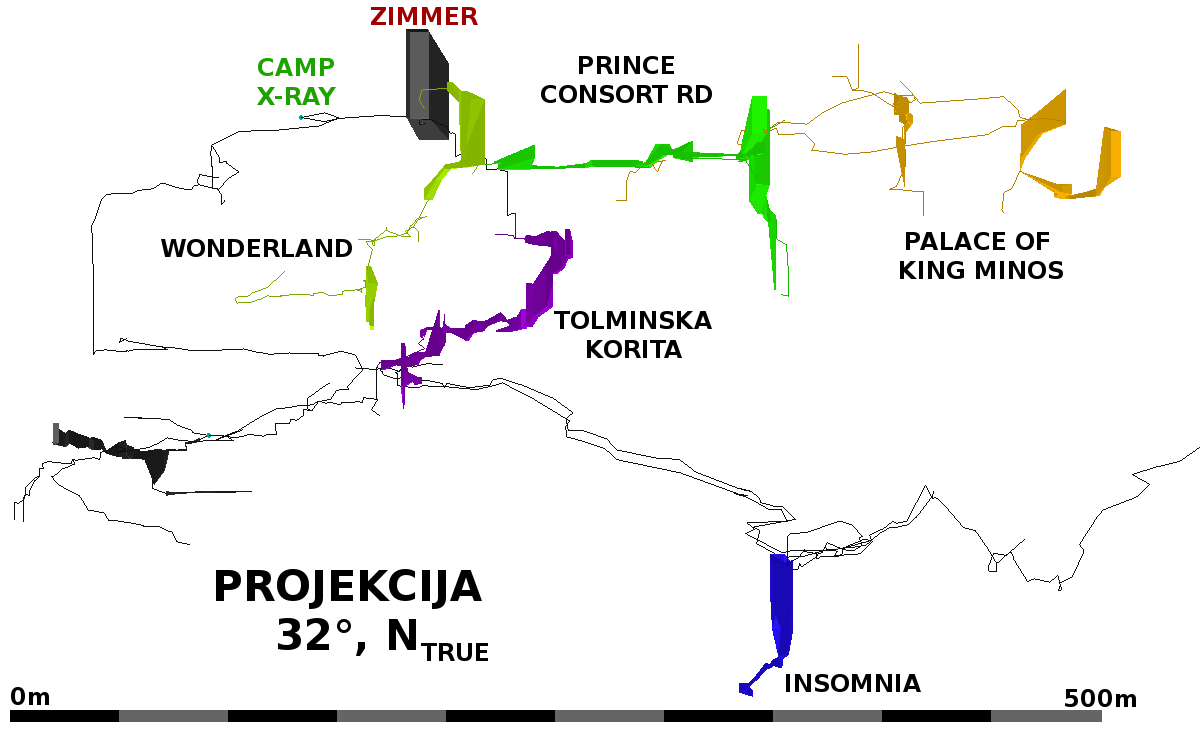
\includegraphics[width=0.85\columnwidth]{2010/2010_deep_vrtnarija_colour_coded_inverted_labelled}
\caption{Colour coded diagram of new cave discovered \& surveyed in 2010 in
Vrtnarija.}
\end{figure*}

\hypertarget{expedition-findings-1}{%
\section{Expedition Findings}\label{expedition-findings-1}}

The initial effort of the expedition was directed into setting up
underground camp.

As the first pushing trips from this underground camp came back with
positive news, exploration based from camp (i.e. deep in Vrtnarija)
quickly became the main focus of expedition effort.

This came at the cost of further work in bounce trips down Captain
Kangaroo (Vrtnarija, the likely connection region to M2) and M2 / SysMig
itself.

The usual surface bashing continued, looking for new cave systems on the
plateau. A revisit was made to the area north of Kuk. This region is
heavily cratered with clear cave development, but the fear is that the
limestone is too broken and chossy for a human sized entrance.

We first visited this region with a serious aim of cave exploration in
2008, and returned in December 2009 on a `winter recce' by a two person
team with ice axe and crampons to identify which surface features were
actively linked into extensive underground systems through the holes
blown in the snow. Several more entrances were identified during this
recce, ones that were likely to be continued to be ignored in the summer
due to their unusual position.

These entrances were relocated (by GPS) this summer, but no new descents
were made.

\hypertarget{leopard-1.5-km-of-new-passage}{%
\subsection{Leopard --- 1.5 km of new
passage}\label{leopard-1.5-km-of-new-passage}}

\begin{figure*}
\centering
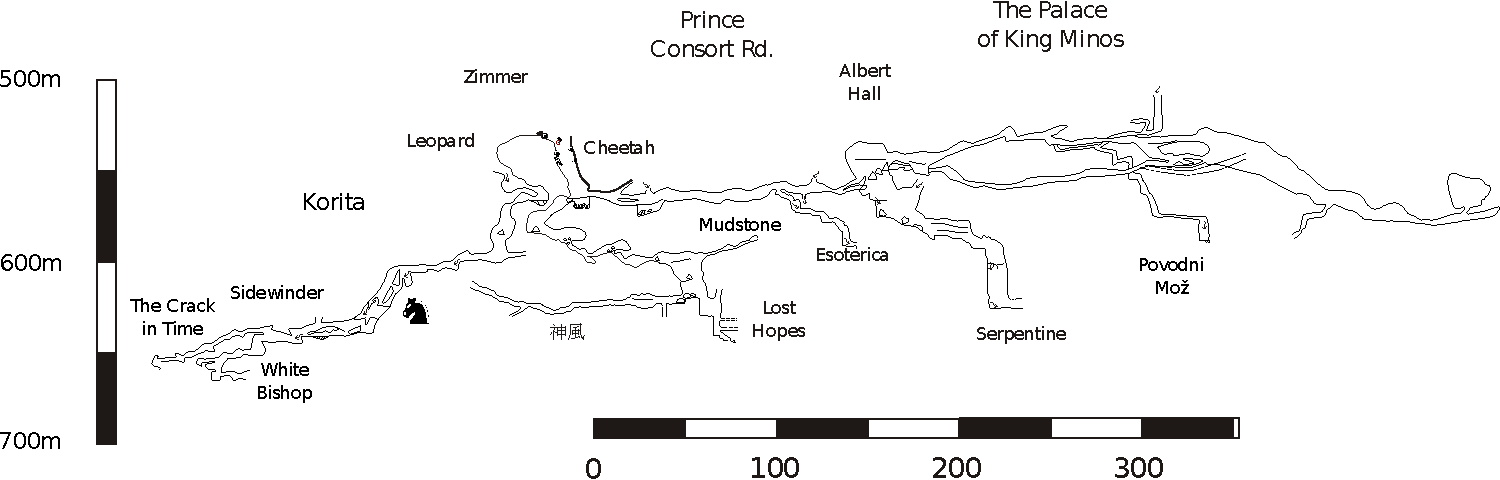
\includegraphics[width=0.9\columnwidth]{2010/2010_new_stuff_extended_extraction}
\caption{Extended elevation of new cave discovered in \textsc{TOLMINSKA KORITA} and \textsc{PRINCE
CONSORT} during 2010 Expedition.}
\end{figure*}

Leopard became the great focus of exploration this year. This lead (a
window off \textsc{Zimmer} chamber, now a 15 m `up' pitch) had also been
originally discovered in 2001, but the drop that it led to had lain
untouched since then.

This was partially due to its loose and muddy nature, but also that deep
exploration had concentrated on good leads elsewhere (most particularly
the lower Vrtnarija level accessed with the bottoming of
\textsc{Big Rock}). This pitch took several sessions of rigging and
gardening to successfully conquer, and is now named Cheetah (P35m),
because of the sense of having cheated death that it engenders on
passing
\footnote{As with other loose pitches, this stabilised considerably over
the next few years.}. There are several windows off Cheetah, which are
definitely promising
\footnote{One was revisited by Jan and Kate in 2011, and found to be an alcove.},
although not easily accessible because of the broken nature of the rock.

At the bottom, this pitch intersects a horizontal, fossil passage, which
can be divided into three main horizontal areas:

Wonderland (heading South) linking into Rolling Stones, Surprise,
Mudstone Traverse, Kamikaze and finally Lost Hopes. This is mainly dry
with large breakdown chambers.

Prince Consort Road (heading North) was initially pushed to
\textsc{The Albert
Hall} (from where the \textsc{Serpentine} meander leads off to the
\textsc{It
Will Rain for a Million Years} pitch). This passage bisects three
streamways (one of which was pushed and forms the Esoterica series) and
includes considerable calcite formations.

From \textsc{The Albert Hall} a climb was made into the
\textsc{Palace of King Minos}. This passage is complex, and side
branches have neither been fully explored nor surveyed. The known
passage leads via Minotaur Rift to terminate in the Queens Bed Chamber
where the draught disappears towards the ceiling.

Together this passage leading off from Cheetah has been explored to over
1.5 km in length, and we are sure that more is yet to be found.

A significant volume of air flows through these regions, indicating that
there may be further developments.

\hypertarget{wonderland}{%
\subsection{Wonderland}\label{wonderland}}

Wonderland is the southern-most of the horizontal development, leading
directly off from Cheetah. It was pushed to a small pitch dropping into
a boulder filled chamber, Rolling Stones, which was the limit of the
first exploration trip due to the lack of rope. This chamber is situated
right below Zimmer, about 40m deeper. There is a further, as yet
unpushed, pitch going down between the large, seemingly unstable,
boulders on the floor.

A happen stance crawl behind some boulders led to further drafting
passage (Hidden Surprise), which, after traversing another chamber and
crawl, finishes in a chamber with a massive hole in the floor (Kamikaze
pitch). The passage continues on the far side of the pitch (traversed on
mud along the left wall), however, due to the collapsed ceiling, these
developments are almost two-dimensional (Mudstone Squeeze). The squeeze,
which is filled with interesting fossilised mud formations, was pushed
to the limits of comfort, although it still continues.

Kamikaze consists of a series of small ledges. From the second ledge a
tell tale breeze led to an interesting bedding plane crawl pushed upwind
but still untouched downwind. The pitch was bottomed (Lost Hopes),
wherein an inlet was followed down a 10m pitch to a series of squeezes
and rifts which quickly became tight. There is a ledge halfway down Lost
Hopes, with a perhaps larger abandoned rift.

These three leads (Kamikaze, Mudstone, Lost Hopes) are of interest as
they now form the most Easterly extent of Vrtnarija at depth, seeming to
`spear' through the large N-S geological feature that contains the
majority of the horizontal passage.

The whole area of Wonderland is extremely dry, quiet and rather spacious
in its scope. It is particularly reminiscent of the higher level passage
in the Easegill system, Yorkshire.

\hypertarget{prince-consort-road}{%
\subsection{Prince Consort Road}\label{prince-consort-road}}

Prince Consort Road is the passage going north from Cheetah. Several
small streams intersect it and some formations have been found. The
discovery of stalactites covered with helictites proved particularly
exciting! The passage leads to a small boulder choke which was easily
passed and led to a large chamber (the Albert Hall).

Before the Albert Hall, three apparently unique streamways have been
found:

One intersecting the passage along a traverse (water chokes into boulder
floor), then around a small chamber at about halfway to Albert Hall, on
a corner of the main massage approximately 2/3 of the way to the Albert
Hall a small rift to the east, and a nice white-sanded water inlet to
the west. The latter leads to an unpushed pitch under the main passage,
there is a cairn and note mentioning the lead. Of these, only the second
has been pushed, into the Esoterica series. Strangely this wet, tight
rift has only been visited once during the expedition, even though it is
still going.

In the Albert Hall two streams enter the chamber from on high (the
ceiling was measured as being over 30m up, by laser disto) and join into
a rather beautiful spacious vadose streamway (The Serpentine).
Serpentine was pushed and leads to another split pitch (It Will Rain for
a Million Years \textemdash{} pushed during a continuing flood pulse).
At the bottom of It Will Rain pitch the stream continues and has not
been explored.

\hypertarget{the-palace-of-king-minos}{%
\subsection{The Palace of King Minos}\label{the-palace-of-king-minos}}

North from the Albert Hall a muddy climb lead to The Palace of King
Minos. This passage and its continuation (The Minotaur Rift) has some of
the most beautiful formations found on Migovec to date, in particular
fine walls of calcite, gypsum and aragonite crystals, mud formations and
weird soot encrusted floors. The Palace has a labyrinthine nature with
several passages leading back to Albert Hall, the largest loop of which
was named Ouroboros

The passage has a classic large phreatic lozenge shape, with some parts
undercut by fossil vadose passage. Near the start of the passage a
significant breeze blew through a small hole. This was enlarged and
found to lead to a small phreatic tube which bizarrely led into an
active vadose streamway (Povodni Mo\v{z} \textemdash{} Water Nymph).
Povodni Mo\v{z} has been pushed upstream to a large active aven (and
smaller dry parallel shaft), and downstream to a sump (approximately
2mx2m in size in the corner of a small chamber and taking the small
flow) and has hence been derigged.

Continuing along the main Palace passage several horizontal tubes have
been explored which lead back into the main passage, though not all have
been entered in the survey. Eventually the main route leads to a high
and wide rift (Minotaur Rift \textemdash{} 20m high, 60m long) beyond
which the best formations are to be found. This passage has a few
interesting leads in it: a high, dry, circular, muddy window to the
right of the passage near a tiny inlet, 2 small tubes leading off the
main passage which both need a little mechanical persuasion.

The chambers beyond Minotaur Rift are spacious and display massive
amounts of crystal formation on all available surfaces --- there is
white `popcorning' almost everywhere, with regions of more intricate
needle and feather formations. The chambers decay into a crawl, which
almost unbelievably is over a smooth calcite floor. This leads to a
classic boulder choke gallery (choking at the end). On the left a small
boulder choke climb leads to the Queens Bed Chamber. In this large room,
the draught appears to disappear up towards the ceiling - both ends of
the chamber are potential climbing projects (\textasciitilde\{\}+20m).

The region is extremely reminiscent of Ogof Ffynnon Ddu II in Wales.

\hypertarget{tolminska-korita}{%
\section{Tolminska Korita}\label{tolminska-korita}}

This lead of Zimmer chamber had been discovered in 2001 but had lain
unexplored until last year, when the first few pits of the active
meander were pushed to a larger pitch. Korita developed into cascades of
active pitches (Black Knight series) to a duck. The duck was soon
bypassed by a 5m free climb into old phreatic level.

The passage beyond soon diverges into two continuations:

\hypertarget{sidewinder-crack-in-time}{%
\subsection{Sidewinder, Crack in Time}\label{sidewinder-crack-in-time}}

The higher dust filled dry phreatic level (Sidewinder, Crack in Time)
connects into \textsc{Envy} in the low level via free climbs and two
small pitches. It is not particularly surprisingly that the `Crack in
Time' was not explored from below, as the connection is made by a long
body-sized crawl above a thin (5 cm) crack connecting to known passage
(Envy), which happily pops out at the top of a obscure 3 m free climb.
Connecting into a 2004 era permanent survey station, Korita now forms a
second loop in Vrtnarija, forming Vrtnarija into a figure-8 shape with
Friendship Gallery at the waist.

\hypertarget{white-bishop-stalemate}{%
\subsection{White Bishop, Stalemate}\label{white-bishop-stalemate}}

The active streamway descends two 10-15 m pitches connected with a
spacious meander incorporating free climbable cascades, before ending in
an impassable rift (-662 m).

This water disappears into `blank mountain' on our survey, but would
require considerable effort to progress, and Korita was thus derigged.

\hypertarget{roaring-floor-tease-muddy-window-off-happy-monday}{%
\section{Roaring Floor Tease (Muddy Window off Happy
Monday)}\label{roaring-floor-tease-muddy-window-off-happy-monday}}

This was regained by bolt climbing from the bottom of Happy Monday to
regain the Muddy Window.

The climb in the mud chamber was made, but quickly led to a large
boulder blocking the way. A tight rift taking a large draught was left
unpushed. Progress is believed to require expansion.

Similarly the traverse to an inlet on Falls Road, and the continuation
of Falls Road itself was left unpushed. A small dig was made in
Friendship gallery beyond Prima junction, which led to a small unpushed
pitch above a stream.

\hypertarget{deep-leads-below}{%
\section{\texorpdfstring{Deep Leads (Below
\textsc{Big Rock Candy Mountain})}{Deep Leads (Below )}}\label{deep-leads-below}}

\hypertarget{insomnia---republika-streamway}{%
\subsection{Insomnia - Republika
Streamway}\label{insomnia---republika-streamway}}

Last year a `written off' streamway (Republika, leading from Red Cow)
was found and pushed upstream to an aven fed watershed, then down the
other limb to a rift pitch.

With the promise of being one of the deepest points of the cave a return
in 2010 was obligatory. The pitch was found to be 41m and was pushed
down a continuing active rift (Insomnia). The end is now only 4m higher
than Colorado Sump (the deepest known point of Vrtnarija). Since the
limit of exploration is above a small 4-5m pitch it is understood that
in 2011 this will inevitably become the deepest passage in the system,
and the signs are good for continuing development of depth. The end is
802m below the entrance of Vrtnarija, but the M2 (Kakna Jama) entrance
is 75 m higher still, and a connection between the systems would make
this point -877m deep overall, with potential for further depth
extension.

\#\#\#Balamory

A return to Balamory was thwarted by lack of rope of the exploratory
party (one more pitch than expected on route), but the team made good
use of the trip to the depths by recovering the camping mats from the
deep 2004 camp (The Fridge, near Cactus Junction), and prospecting for
other leads with some success.

\hypertarget{original-exploration-stories}{%
\section{Original Exploration
Stories}\label{original-exploration-stories}}

\hypertarget{rerigging-vrtnarija}{%
\section{Rerigging Vrtnarija}\label{rerigging-vrtnarija}}

An early morning on expedition\ldots{} I stumble my way down to the
Bivi, late as ever, and set about fixing some coffee. It's a disturbing
hive of activity. William and James KP are planning to rig as far as
possible, replacing the rope below Pico with new and rebolting where
necessary, Tetley is following them down and introducing the new cavers
to Vrtnarija.

Excellent! Everything is in hand. Gergely suggests we follow up the rear
with extra rope and rigging gear, preparing the ground for tomorrow's
deep pushing. Looking forward to a nice, relaxing, afternoon trip, I
don't bother to cram food into myself (I'm never that innately hungry in
the mornings), and Gergely and I take the minimum of provisions.

It's nice to be back in Vrtnarija again, after a year, and even the
stepping aside on the pitches to allow the vast quantities of cavers to
pass is fine. Eventually we pass everyone else \& get to Swing, and find
William and James KP. They're both pretty pissed off, putting a new bolt
in on Swing and rigging the blasted thing has sapped their energy.

So Gergely and I take over. I rerig Tesselator, coiling the old rope
ready for recovery. The head of space odyssey receives an extra bolt and
thus a Y-hang, originally I intend to remove the deviation entirely, but
find that I've misjudged slightly and it's still required, just.

The traverse ledge halfway down space odyssey needs more work. Gergely
comes down and we work on it together, me putting in more bolts and
working new rope out along the traverse, whereas Gergely carefully
walked out on the old traverse and rigged the pitch down to Concorde. We
have a bit of confusion in the middle, as we also have to start a new
rope. All sorted out, we have a spare 15m of traverse rope that we hide
for future use in a cubby hole.

Leaving the bolting kit and rope for future riggers, we have a smooth
exit. Rather deeper and more effort than I had been intending for this
first day's trip, and I was certainly feeling the lack of food as I
prussic'ed back up the entrance series, but successfully completed
nonetheless. In their first day of caving the expedition had rerigged
down to -300m!

\attrib{Jarvist Moore Frost}

\hypertarget{the-discovery-of-wonderland}{%
\subsection{The discovery of
Wonderland}\label{the-discovery-of-wonderland}}

It was another rainy day. Arriving not too long ago to the plateau, the
thrill of the new possibilities for discovery was boiling in my venes.
While drinking incountably many cups of tea, we discussed the
possibilities with the old lags who are always the source of infinite
wisdom. Dave suggested to check out Leopard, the passage that opened
from Zimmer, just opposite of Friendship Gallery. Martin McGowan had
been there some 10 years ago, but information was unclear, and the
chances for the continuation there had been at least dubious -- so given
it is so close to camp, why not give it a go?

Andy was sort of up to going underground, and I felt super happy to go
caving with one of the heroes of the discovery of many underground
passages on Mig. So the usual endless faffing started, packing good
amounts of food, Vitaminski, gas canisters, and some Zganje, and
finally, well in the afternoon, we started our descent towards the
unknown.

The way down we got again used to the feeling of hanging in big abysses
on dubious bolts, which proved to be quite useful for what followed.
Reaching Zimmer, Andy chatted to Tetley and Myles (who were already at
camp), while I bounced with the rope to the window and put in two bolts
for having an easier start the next day. Having a sleep at camp was OK,
although Andy did not seem to be very happy about the limited comfort of
X-Ray, and he stated that he was too old for underground camping -- a
fact that changed little of our plans for the next day, of course.

So, in the morning we climbed up to the gallery, and secured the rope to
a large boulder at the top of the climb. Leopard was very nice, a
typical phreatic tube, with formations resembling the spots of a leopard
on its walls, and also with a fairly good draught (I am always keen on
following the wind). At the other end, a dark muddy pitch-head waited
us, with a good number of scary, loose boulders around it. We again
noticed that Gardeners' World is so aptly named, and started to clean up
the place. We could not remove the largest rock, tilted against the
wall, so decided to go underneath it. We were not quite sure that it is
going to stay, but it is still there, after hundreds of cavers have
passed beneath\ldots{}

I took the nice 9mm rope that we packed, secured the end around a big
boulder in the passage, and started the descent. The slope was terrible,
completely muddy and also full of loose material. Luckily, I managed to
put in a bolt in a piece of bedrock on the right side that popped out
from the debris. Then, descending through the narrow window, a large
chamber opened up beneath my legs. It was absolutely terrible.
Everything I touched fell down instantly, starting a small avalanche of
loose rocks. I managed to put in one deviation, and then, after many
failed efforts to put in a rebelay, I finally descended down to the
bottom of the chamber, where, to my amusement, I saw some little
stalactites, and great passages starting off. I cleared off from the
bottom off the pit, and Andy followed very carefully. When he reached
the bottom, he asked me in his typical sarcastic style, if I knew that a
rub-point can cut a 9mm rope already during only one descent. Well,
sure, but it already survived two, so no problem! - I replied. We built
a cairn at the bottom for easier surveying, but no traces of it remain
now. The pitch caused quite a trouble for a long time -- due to its
unforeseeable nature, it later got the name ``Cheetah''. Finally, after
some years' time of usage, it seems to stabilize, at least let's hope
so\ldots{}

So, we started to discover the big passages that laid ahead. Little did
we know about the many kilometres hidden behind them, but we felt that
we got into something different, something very old, and it was very
exciting. Andy recalled that he had found a lot of large vertical
pitches, despite the fact that he hates big pitches -- so finally, he
was eager to find something horizontal! First, we went to the large
passage that opened towards the right. We followed it for about 200
meters, with small drops, and we finally reached a bigger drop that lead
to a chamber filled with rocks. Unfortunately, our rope was too short
(although we even made use of the chords of our tackle-sacs), so we
could not descend there. Mirroring our surprise, we named this part
Wonderland, and went back to the first pitch. Starting in the other
direction, I put in a small traverse line with its middle belay at a
small waterfall, and reaching the other end, we saw that Andy's dream
finally became true -- we found a true horizontal passage, whose ceiling
was covered with small crystals! (Since then, experience showed that
these are typical wind crystals, indicating the way of strong draught --
and here, indicating the way towards the Connection, although that is a
different story\ldots{}) Hurrah! We followed the passage eagerly, and we
were even more amazed when it opened up to a junction. A flat-out crawl
lead to a nice little chamber, whose ceiling was full of little
crystals. On the left, we also found a pretty water inlet, filled with
white sand. Underneath the main passage, we also climbed down to some
openings where water could be heard in the distance, perhaps 40 m below
us. Finally, we reached the place which seemed to be the termination of
the passage - a boulder choke. Hmm. We soon managed find a way upwards,
and when popping out at the top, we suddenly found ourselves in a big
void! Wow! A big chamber! With a waterfall! And a window! And another
window! And an obvious continuation of the phreatic! Andy asked if I
knew of Exhibition Road in the system, and that this was similar to
that, so we decided to name it Prince Consort Road (later, quite aptly,
it got renamed as Albert Hall). By that time, it was quite late, and we
had to start back to survey, but we did it happily. Finally, quite
broken, we prussiked up on the very dubious 9mm rope, took it up so that
no other person repeates the same insanity, and walked back triumphantly
to X-Ray.

Andy's words in the logbook express the essence of the day: ``AJ and GA
turned one crappy lead (Leopard) into lots of great leads''. That's what
perfect cave exploration should be, isn't it? Well, our luck has proved
to be good, once again\ldots{}

\attrib{Gergely Ambrus}

\hypertarget{pushing-insomnia}{%
\section{Pushing Insomnia}\label{pushing-insomnia}}

I had travelled down to T'min to clean and get over the cabin fever that
develops over the weeks of life on the Plateau. That night, after a slap
up meal and a few bruskies, Jan arrived and we had a great evening of
beer and bullshit. After the beer, we passed on to the whiskey and the
bullshit got increasingly epic. ``The leads at the bottom of Red Cow are
going to make GW deeper'' I told Jan ``the next pushing trip will
definitely do it''. So after walking up the hill having dinner and a
little too much to drink at the bivi we set off for the night train.

Soon enough we are at camp and decide to keep going down, looking to
continue pushing the Republika lead. I must admit it took a lot of
strength not to push the leads that were already multiplying near camp,
but I knew the way to Red Cow, having been there with Dan a few days
earlier. We soon got to the junction and followed the water upstream.
Nice caving, I start feeling the all familiar excitement: here come lots
of km of fresh cave!

At one small pitch I turn around and find Jan has disappeared. I turn
back to look for him and find him wandering in the wrong direction
towards the sump. Apparently he had fallen asleep and started wandering
off route. Shit maybe we are too tired for this? Meh! We get to the
pitch head for Republika, which I must admit is rather God forsaken and
wet and awful. We drop the pitch, I get the drill out and start rigging,
brain totally disengaged. As I am rigging I can feel the batteries
getting weaker and weaker. I guess there were a few too few bolts at the
bottom of the main drop and maybe some of the pitch heads could have
been a little neater. It certainly helps to cave with a tall bastard is
all I can say :D.

We reach the bottom of the main new pitch and it's a rather God forsaken
wet and damp place. The water keeps going down along some immature
passage. We follow the water, noting at least one unlikely but unchecked
possible side passage. A few hand lines are placed here and there and
the drill battery finally dies. Just as well as the last pitch we get to
looks like a right nightmare: really tight pitch head etc. By this point
we realise it's super late and we are almost certainly going to miss our
callout. Time has gone in a blur, we are probably not 100\% there
mentally to be honest. Still might as well survey out.

The way out is not very remarkable. We bump into Tetley at the top of
Big Rock. He is not too worried, but apparently Gergely was hoping we
were crumpled up in a heap somewhere so he could come and rescue us.

\attrib{James Kirkpatrick}

\hypertarget{more-horror-with-jan.}{%
\section{More Horror with Jan.}\label{more-horror-with-jan.}}

The next night we get up and decide to do some pushing. The whole day is
marred by the fact that - once again - we promised not to push the
obvious continuation from Albert Hall. So we decide to have a random
bimble around. We try looking for alternative ways around the Albert
Hall. No success. Somehow we end up pushing a lead from the right of the
passage leading to the Albert Hall (right looking towards the Albert
Hall!).

The passage is small and bends under the main route. It is wet and
rather grotty. We drop a pitch or two of utter horror and eventually
turn around. Surveying out is awful. The book gets wet, my fingers are
too cold to hold the
instruments\footnote{The survey data had to be 'corrected' to avoid the survey self-intersecting due to backwards legs.}.
It sucks majorly. At least the passage gets a cool name: Esoterica. O,
and no-one has pushed the pitch where we stopped!
\footnote{Esoterica was not revisited until 2012, where a broken bolting driving prevented any additional pitches being descended. 
It remains a lead.}

\attrib{James Kirkpatrick}

\hypertarget{happy-days-with-jan.}{%
\subsection{Happy days with Jan.}\label{happy-days-with-jan.}}

On our last day together we went looking around the amazing passage that
we politely left for Dan and Izi. We smashed our way through the
entrance of what would become Po Vodni Mos, we looked at the Queen's bed
chamber, we pushed down some random tubes at the sides of the main route
(has anyone ever surveyed these I wonder, one of them went!). All in all
a super chilled day. No surveying and no water. And then we got back to
camp, watched some videos and drank a lot of whiskey, Happy Days!

\attrib{James Kirkpatrick}

\hypertarget{balamory}{%
\section{Balamory}\label{balamory}}

When James and I went to have a look at the bottom of Balamory on the
first day of our one-noght camping trip, we didn't make it to the target
as an unexpected first pitch used up too much of the rope that we had
taken with us.

However, as well as airflow going towards Balamory, there is also
airflow in the main passage above, beyond the point where the hole down
to Balamory leads off so here are two leads in that area there that are
worth looking at.

The upper lead \emph{does} need some way of climbing across a pit to a
ledge covered in loose crap (maybe a bolt traverse round one of the
walls, though I can't remember how much good rock there was in that
area.

Subsequent email exchanges on the subject do seem a bit vague as to
exactly what was done, and whether the upper passage had actually been
boldly examined or not (Clewin was bold somewhere round there, but it
wasn't certain where), but anyone going to potentially move/split the
boulder down Balamory (I think it was supposed to be down the third of
the three possible `second pitches') down should also probably plan to
look at the upper passage continuation, especially if they have a
drill/bolts to help with climbing/traversing belays.

On the way back from this little trip, after grabbing some stashed
karrimats from the old camp, that the black black hole across Big Rock
was noticed.

The next day, James and I went to the new stuff below Leopard/Cheetah,
but since we were doing a push-then-out trip, rather than going to the
far end of the `half' where most of the action was, we went in the other
direction from the pitch bottom to do some work relatively close to
camp, carrying on where Gergely+???? had left off at the Hidden Surprise
pitch.

Gergely had dropped the first section of the pitch to an obvious ledge
and followed the ledge to horizontal passage that soon died. James and I
were to descend the shaft from the ledge, but it immediately became
clear the drill wasn't working and so we had to resort to spits, with
James bolting while I waited on the ledge.

Fairly soon the bolt (bolts?) was in and James had descended to a large
boulder-covered ledge part-way down the large shaft, where I could
safely join him. Some of the boulders were rather large, with gaps
between them or between them and the wall large enough to climb down and
move around in. While James did the business with the next spit, I
wandered around between the boulders to keep busy. Where the boulders
met the wall, the wall was somewhat overhanging, and from the lowest
easily-accessible place near where I had first climbed down, it was
possible to look between the boulders marking the lower limit of easy
movement and the wall to see a few metres away/down to where the wall
seems to meet the proper floor of the ledge, where there was a layer of
white rock flour, with some potentially human-sized space between me and
it though with no obvious way to get there.

From where I was, looking along the wall `clockwise', it also looked
like there was a space of some sort ahead of me horizontally, but
getting to it didn't look very nice, and after all, I was just in a pile
of boulders on a big ledge half-way down a pitch, not in a classic
boulder choke as such, so there seemed little point doing anything
borderline just to get to a slightly different place in the boulder
pile.

However, just as I was preparing to go back up and see how James was
getting on, I breathed out a large sigh, only to see it get sucked
horizontally away from me between wall and boulders and into the space I
had been looking into, which immediately aroused my curiosity.

To get into the space I could see required going horizontally through a
not-quite-body-sized vertically-rectangular gap with a short (1m) drop
on the other side. After removing all my SRT kit, and doing some work
with a convenient rock hammering edges off the boulder forming one side
of the slot to make the gap wider, and progressively blunting sharp
edges on the wall side as they proved awkward when attempting to get
through, it was possible to slowly and delicately post myself through
feet first and eventually emerge free on the other side.

Turning around, a short crawl led to a wider area under the overhanging
wall, and a view ahead to where the wall/roof sloped nicely down towards
into the floor to leave a wide bedding plane with clearly no way on.
Turning around somewhat disappointed, the main wall, which I had been
looking away from when I had initially turned round, was seen to have a
crawling-height hole in it, which, on approaching, it was clear most of
the draught was going into.

That hole led to a small chamber with a further hole leading in turn
into the side of a walking-height passage with a good breeze running
along it. The draught I had followed initially was clearly just a
tributary being sucked into the main airflow.

I quickly returned to James to tell him of the find, and we decided to
do a little surveying and exploration. We chose the upwind branch which
didn't run a great distance before ending in an upwards bedding-plane
slope ultimately blocked by a large slab in the bedding blocking
sideways movement into what appeared to be a chamber with a waterfall
entering. Capping or plugs/feathers would seem to be needed to shift
this blockage. On returning to our entry point, we looked the other way,
wondered how far the downwind passage went, but left it for someone else
to explore.

We hadn't found a great deal of length, but on the other hand, we had
left a decent going lead, and due to the combination of a misbehaving
drill making waiting cold and dull work and the luck of my breath
showing there was something worth looking at, had ended up finding quite
interesting passage in what must be one of the most unlikely of
situations.

Thinking partly of the initial nervousness with which I had slowly
posted myself between the boulders and the wall, but mainly of the
immense luck we had had with the draught, Kamikaze seemed like the
obvious choice of name for the discovery.

\attrib{Dave Wilson}

Last year we manage to connect Captain K. with lower parts of Vrtnarija
(friendship gallery), so I could not wait to go caving again, especially
to first descent the whole Pico.

Dan and I decided to go camping in X-ray, which was after re-established
after many years.

We were on the night train. So the plan was to go caving late at night,
reach the camp in the morning and then go straight to bed. When we
reached the camp we find a note, asking if we could wait a bit longer,
because the other team return late. We decided to go and check out the
newly discovered parts and maybe find some leads for tomorrow. When we
return to X-ray we meet our tent mates Gergely and Niko, who just return
from their caving trip. We prepared some food, change to dry clothes and
went into sleeping bags, while others started preparing for caving. It
was funny to watch how they were not happy to put on wet caving clothes.

\attrib{\izi}

\hypertarget{palace-of-king-minos-queen-bed-chamber-minotaur-rift-and-ouroboros}{%
\section{Palace of king Minos, Queen Bed chamber, Minotaur rift and
Ouroboros}\label{palace-of-king-minos-queen-bed-chamber-minotaur-rift-and-ouroboros}}

We were woken up by Jarv and Jan who just return from their pushing
trip. While cursing wet clothes we discussed what they find and what is
worth to go and push. Soon we took off and separated on the bottom of
Cheetah. Gergley and Niko went down Wonderland, Dan and I went to Prince
Consort Road. Road lead us to Albert hall where not long ago Jarv and
Jan were pushing Serpentine. We decided to push some new leads, so we
climbed higher in this chamber and from there we saw a big gallery. To
reach this gallery we needed to climb about 6m high. Dan gave me a push
up and I was able to reach the top. There I secured the rope around the
bolder and Dan joined me. From there we made a traverse and then entered
the gallery. Already on the entrance we noticed something amazing. The
ceiling was covered with white crystals, that we never accounted before.
That meant this is an old phreatic gallery and we were so lucky to be
the first one to discover it. Also the soil on the ground was brown on
top and once we stepped on it, it was white underneath. Our first steps
left white trails of footsteps behind, truly amazing. We were really
careful with our steps, as we did not want to make to much damage. We
mainly stick to the main passage and there were no pitches or tight
squeezes, perfect for exploring. On the end of this gallery we were
stopped by an aven. We could not climb it, so we decided to return and
start surveying back. On the way back we took another side passage which
lead us back to Albert hall. Because we made a loop and the hole place
look like a maze, we name it Palace of King Minos, the side passage was
named Ouroboros, cuz it was a loop to Albert hall and also we named the
big rift Minotaur. We left one side passage for next time, because we
were already tired. Surveying this gallery was a pure joy. Long
distanced between stations, minimum of 10 m. Both of us were extremely
happy with our discovery and so we return to X-ray for well deserved
rest. In the camp we meet the other team and also they find some new
meters. We exchange our trip experience and fall a sleep.

When we woke up, we were surprised by roaring in Zimmer. During the day
it was raining outside, therefore a lot of water was purring down
Zimmer. Dan and I still have one more night at a camp, but because Niko
and Gergely were not feeling to go out in these conditions, we
volunteered to do it. Beside, someone had to cancel their call out. So
we eat something and start going up to the surface. I was first heading
out, but before I fully attached myself on the rope in Zimmer, I was
already all wet. I told Dan that I will not wait for him and because we
both know the way out, we will see each other on the surface. I was
going for about an hour, stopped, roll 2 cigarettes, smoke one, and
leave one for Dan and then continue out. Below Pico, I repeated the same
procedure, so at that time Dan catches me up and we continued together.
Above Pico it was less water so that meant that the rain has stop. We
reached the surface in 3 and half hours. In the bivy we entered the data
and we were so happy when we heard that we surveyed more than 500 m,
especially how easy was to do it.

\attrib{\izi}

\hypertarget{hidden-surprises}{%
\section{Hidden surprises}\label{hidden-surprises}}

Well, the name \emph{Wonderland} does not really exist anymore, but back
then this was used for the horizontal level at the bottom of Leopard.
Once finishing our triumphant trip with Andy, I was eager to get back to
continue the exploration of the many passages that lay below. So, we
paired up with Niko, to form a truly Eastern European team, and went
back to do what we had to do -- rig the drop at the end of the
\emph{Wonderland} passage!

Izi and Dan went to the other end, to find the continuation from the big
chamber (Albert Hall). With Niko, we improved some of the rigging that
we did with Andy, and then dropped to the chamber with loose boulders.
Unfortunately, the rope that I used was new, and it shrunk considerably
later, so those rebelays have been too tight ever since. Within the
chamber, we climbed down to the obvious continuation, to find to our
horror an incredibly loose pitch within a pile of incredibly loose
boulders -- so we agreed that this was not the best option, if we still
want to do something else with our lives. Nevertheless, this experience
provided us with a good name -- Rolling Stones! So, there we were, in a
nice big chamber, with a suicidal way onwards, and we were not quite
keen enough to continue that way\ldots{} We had a look here and there,
to no avail, and were about to turn back, when Niko climbed in between
some rocks, and said in his usual slow manner -- ``Heey maan, maybe this
is the right waay, nooo?'' And indeed it was! Following the draught, we
soon managed to open up a small passage, which lead to a flat-out crawl,
but after some 20 m it again popped in to another chamber, quite nicely
decorated. Hidden surprise! That was the name we chose. The way on was
obvious, and soon we emerged at the top of a large black void space.
This was a good point to turn back, so we surveyed everything and showed
it proudly to the happily emerging pair of Izi and Dan. Then we returned
to camp together, shared a nice meal, talked about our stories, and had
a nice evening, as usual at Camp X-Ray.

Next day, we went back with Niko to the top of the pitch. Two ways were
at the offer: either down to the black, or across to the seemingly
obvious continuation of the phreatic tube. I was quite scared of going
down, so we chose the more safe option of doing the traverse. Niko put
in his first ever bolt at the Milka rock (which resembles a cow), and
then we slowly proceeded, given that the whole thing was done by hand
bolts. Finally I climbed up the slope on the other side (quite a scary
experience), and we were there at the start of kilometres of a wide,
walking phreatic passage! At least, we believed so. This expectation
proved to be immediately wrong, when after 15 m, we had to take off our
SRT kit in order to pass a squeeze. Never mind, we thought, the walking
passage is just on the other side! Well, not quite\ldots{} the ceiling
got lower and lower, and we really had to fight to advance about 50 m.
There, the passage became really low, so we decided to try to survey
back. It has been a gymnastic feast, not only small and low, but also
super uncomfortable because of the dry, fossilized mud formations that
filled the floor completely. Niko was super happy to be there -- the
afternoon was mostly passed by his constant ``Noo, maan''
moaning\ldots{} The mud formations are indeed very nice, maybe they
should be scientifically investigated. Anyway, they gave the place a
name -- Mudstone Squeeze and Mudstone Traverse were what we surveyed
that day. To this date, nobody has been back to Mudstone squeeze --
although it is quite a place to go, if you happen to have some free time
and want to exercise your squeezing and crawling skills! ☺

Back at the camp, we heard the great news: Izi and Dan just found 600 m
of passage at the Palace of King Minos! We were about to exit the cave
the next morning, but there apparently had been a great storm, making
Zimmer impassable for a good 20 hours. So we got the opportunity to have
a tourist trip to King Minos Palace, and we did very well to use it- and
absolutely amazing bit of cave! After another night at camp, we finally
started to the surface after 4 days underground, but we were certain to
return to the plethora of exciting leads\ldots{}

\attrib{Gergely Ambrus}

\hypertarget{discovering-povodni-moux17e}{%
\section{Discovering Povodni Mož}\label{discovering-povodni-moux17e}}

After couple of days on the surface, I decided to do some camping with
my Slovenian mates. Tjaša, Erik, Mawer and I started to walk towards the
entrance around 2 am. We reached the camp too early for our bed time, so
we decided to go and check out the crystals. After that we still have
some spear time so we decided to go and try digging in Minotaur rift,
where last time with Dan we could here big roaring of water. After
couple of hours moving boulders with no luck, we returned to camp.

The next day we made a plan to push one lead in Palace of King Minos,
that we didn't push with Dan. The entrance was quite narrow, but soon we
arrived to a series of pitches with water. We had enough of rope to bolt
2 pitches and decided to name it Povodni mož, cuz we followed the water
all the time.

\attrib{\izi}

\hypertarget{m2-kavkna-jama}{%
\section{M2 --- Kavkna Jama}\label{m2-kavkna-jama}}

The JSPDT organised a trip based at the mountain hut at Kal on 2nd
October 2010. The terminal rift was enlarged to gain a \(\approx\) 20 m
pitch and a larger, undescened (due to lack of rope), pitch.

A return trip three weeks later descended the pitch and found it to be
\(\approx\) 60 m. The cave closes immediately, with a tight rift taking
the water and a slightly larger abandoned rift also offering potential.
It draughts strongly.

The M2 cavers returned in thick fog, following their footsteps through
the 10 cm deep snow. With the coming winter Migovec is effectively
closed for exploration until summer 2011.

\hypertarget{exploration-outlook}{%
\section{Exploration Outlook}\label{exploration-outlook}}

In all, 2.2 km of new cave was found during the 2010 Vodna Sled
expedition, taking Vrtnarija to 8.776 km.

We are in the extremely fortuitous circumstance where we finish the year
with considerably more leads in the Migovec cave systems than we started
with. The Vrtnarija camp was derigged with the certainty that we will be
back next year camping in the same location. Gas cylinders and cans of
fish were left sealed in Daren drums with a rock of carbide to keep them
dry, the carry mats and tents were left standing to air, and we have a
considerable armoury of rope brought back from the pushing fronts
waiting for the 2011 team.

The work by the JSPDT in the Autumn has \texttt{opened\ up} M2 once
again and brought the possibility of forging a connection back to the
table.

The pushing of the Republica streamway (now Insomnia) to within a few
metres of the maximum depth of the cave has reawakened the possibility
of further depth extension to Vrtnarija. Expedition members have mooted
the possibility of establishing an additional 2-man `deep camp' to
benefit pushing trips in the lower reaches of the cave, particularly any
revisits to the far North end of the system.

\hypertarget{migovecs-long-term-prospects}{%
\section{Migovec's Long Term
Prospects}\label{migovecs-long-term-prospects}}

It has been a recurrent discussion in our club as to when we will run
out of new cave to discover in Migovec. Almost all of our fruitful
exploration has taken place within a single square kilometre of the flat
topped mountain.

Migovec, being part of a mountain chain that is the first high altitude
interruption to moist air from the Adriatic, receives an extremely
significant level of rainfall. This summer, Jaka Ortar, a Slovenian
geographer, recorded 210cm of rain on Migovec in 100 days (28th July-3th
November) with his network of rain gauges. However we have never found
any large rivers underground --- the known cave can only account for a
tiny percentage of the total drainage for the plateau.

Our current hypothesis is that there is no \texttt{master\ system}
gathering the water, but instead a complex hydrology induced by cave
passage intersecting the underlying (as yet, unvisited) band of
Cretaceous shales.

For all Vrtnarija's complexity, the entire cave can be fitted into a
slab of limestone slanted at 66 degrees and just 1000x150x1000m.

Certainly, as long as we can continue to find entrances through the
frost shattered and heavily cratered surface, there will be enough cave
in Migovec for decades more of exploration.

\#\#Underground Logbook

\hypertarget{found-in-aggregateofmig2007-2010.doc-jarv-typed-up}{%
\section{Found in `AggregateofMig2007-2010.doc' : Jarv Typed
up?}\label{found-in-aggregateofmig2007-2010.doc-jarv-typed-up}}

Camp X-Ray Logbook: After about 6 hours of caving, finally made it down.
Met Gergely \& James on he way down as they were leaving the cave. Last
bolt before camp is horrible = needs rebolting / rerigging. 15cm lower
would be awesome. Built a tent at the camp. Required some stone
movement. Mike got water, me \& Jarv built tent, kate = smoking. NEED
WEED! Should have thought about it before. Listening to Massive Attack
and getting Raptured. Oh yeah! Kate setting up sleeping space, Jarv went
to get more water.

Camp is getting established, looking forward to Worms World Party. Mike
= Cooking. Weed is really a missing resource. So far so good. About 5
metres from camp is a hole with water in it = able to hear, quickly got
established as peeing
corner\footnote{The fast increasing smell of urea put a stop to this practice, and instead a BDH container emptied in Zimmer was used.},
hope its not a lead\ldots{} Nick

23/7/10 Nice snooze - super warm. Nicola snored like a trooper - just a
few minutes into the classic Black Adder session. Broken sleep -
particularly as Nicola got up for X2 piss. Awoken @ 10:30AM by the
beasts crawling up towards our pits. Tetley \& Myles rustled up some
hot-choc then wandered off down the continuing passage.

23.7.10 - 2:10pm MD + Tetley Entered Gardener's World
\textasciitilde{}6:20am. Made our way through, re-rigged zimmer on the
way. Arrived at camp at 10:30am + awakened JV, Mike, Kate + Niko.

Wandered around friendship gallery for hour or two. Found nice lead,
will investigate later. Sleep now.

23-7 2:20pm

It's good to be back in a sleeping bag at Camp X-Ray - seven years since
the last camp here. It's very comfy. I like the tent - some things don't
change though, Blackadder on the sound system, smash + tuna etc.
Hopefully we'll get some good pushing in tomorrow! Tetley

23-7 6:20pm James and Dan arrive for a quick visit before heading off to
push the muddy window 8:20pm Andy + Gergely arrive - I ignore them! Tet

23-7 10:30pm Fucking body won't fall asleep! Must have only had couple
of hours at most since Dan arrived\ldots{} Gergei + Andy turned up at
8ish + now, they have checked our Leopard a little. Tetley's bodily
functions are out of control! May bring some corks down for his
digestive tract next time. Anyway, now for some food + tea + hopefully
can stay awake till bedtime at noon! Myles.

23-7 11pm Myles and I share breakfast / dinner with Gergely + Andy. Fine
food! (Ed: Believe this was Tetley)

24-7 12:20 Breakfast with Tet \& Miles. Dan \& I will visit the lead we
killed yesterday (Muddy Window) \& survey it, then to Red Cow. James K

24-7 1:30pm MD Back in Camp for 2nd night. Pushed Tolminka today, good
lead, surveyed \textasciitilde{}8am. Some nice pitches. Covered in mud.
Listening to strange foreign music.

24-7 2:05pm Great push down Korita today - 8 bolts, surveying etc. IT'S
GOING GOING GOING\ldots{} GO THERE! (But try and avoid rigging future
pitches in or near the water\ldots{}) Andy + Gergely have left to push
Leopard - James + Dan to survey Muddy Window and then go for a jolly
below Big Rock. I've had a great day - thanks Myles. Time for a decent
seep. Tet

23:20 24/7/2010 James + Dan return on a high! 9hrs good kip in bed - I
feel good! forgot to say I had a shit yesterday\ldots{}. Tet

\hypertarget{izgubljeni-raj}{%
\chapter{2011 --- Izgubljeni Raj}\label{izgubljeni-raj}}

2011 was another great year deep within Tolminski Migovec. The weather
was horrendous --- we even had snow! But the cave kept on going. We
found over 2.2km of new passage all below -500m in depth, and took the
cave to a new deepest point of -888m. All of the exploration took place
during underground-camping trips based at X-Ray (Vrtnarija, -550m), with
the keenest of expeditioneers managing a total of around seven nights
underground during the four week expedition.

\#\#\#Introduction

Between 15th July and the 15th August 2011, Imperial College Caving Club
had twenty members participate in the Izgubljeni Raj 2011 expedition to
Tolminski Migovec, Slovenia. The aims for this expedition were the
continued exploration of Vrtnarija, where considerable efforts in 2010
had led to the discovery of 2.2 km of mainly horizontal passage, all
below 500 m in depth. At the start of the expedition, Vrtnarija was 8796
m long and 807 m deep.

This summer we had less manpower than last year, but were still
attempting to set up a similar four-man camp at -550 m and carry out
deep pushing. Our exploration continued routes which were diverse in
direction from camp---soon we were taking many hours just to travel from
camp to the pushing front and back.

As a result of the reduced manpower and the considerable demands that
exploration of Vrtnarija was making on our time, we unfortunately did
not manage to contribute towards the exploration of Kavkna Jama and the
attempted connection of the Migovec and Vrtnarija systems.

Our efforts were considerably hampered by the weather. We had the
wettest summer we've ever experienced on Migovec. We only very rarely
had sunny enough periods to dry our caving equipment and clothes. A
particularly memorable rainstorm of 48 hours near the beginning of
expedition was rounded off by a heavy snowstorm -- the first we've ever
experienced in 15 summers on this mountain!

For two periods of 36 hours, underground camp was effectively cut off
from the surface by high water levels in the cave system, making some of
the pitches impassable. Thanks to the quality, warmth, provisions and
size of underground camp this wasn't a major problem as exploration
simply stopped and the explorers got a lot of sleep instead. Certainly
underground camp was a more pleasant environment than the windswept,
rain lashed and barely above freezing surface of the mountain.

In all we discovered 2229 m of new cave passage taking the cave to 11025
m long and 888 m deep. All these extensions have been made at depths
greater than 500m, on multi-day trips based at an underground camp.
Vrtnarija now has the vast majority of passage, over 8 km, at depths of
greater than 500 m.

\#\#Cave Discoveries

Our major cave finds this year can be considered in three separate
developments within Vrtnarija:

\hypertarget{the-serpentine-let-na-drugi-svet}{%
\subsection{The Serpentine \& Let na Drugi
Svet}\label{the-serpentine-let-na-drugi-svet}}

An active streamway, named the Serptentine, led off from a large chamber
(The Albert Hall) discovered along Prince Consort Road. During 2010,
this was pushed to -621 m (It Will Rain for a Million Years).
Exploration in 2011 continued along this active meander.

The initial exploration (Round Pond) descended a 2m climb down leading
to an oxbow and 4m pitch. The following trip traversed out along a crack
in the ceiling to avoid falling water down a 10m pitch (Longwater) which
entered a chamber (also Longwater) with significant iron deposits (in
the form of heavy \textasciitilde{}4cm thick plates of dark mineral in a
vein within the limestone), and a considerable number of orange-stained
straws and stalactites.

The boulder collapse in this chamber was bypassed by a squeeze between
boulders on the right which entered a crawl-way which soon refound the
water flowing from beneath the boulders. A 4m pitch was reached where
the bedding plane appeared to intersect a joint. A 3m diameter
apparently rather deep pool is present below this pitch. Passage
continues in vadose development with the water, which entered a small
chamber with a set of cascades (cascade chamber). There is also an
apparently phreatic connection between high up in the roof of this
cascade chamber and part way up the 4m pitch.

The cascade chamber is rather complex in structure, the cascades falling
into a large \& deep 4x2m pool. This water flows down a short rift and
immediately tumbles down a \textasciitilde{}8m pitch (Duffers Drop)
which leads via two freeclimbable cascades (requiring very careful
maneuvering near to the water) to reach a wet inlet on a large pitch
(Drink Your Own).

Behind the large pool in cascade chamber there is a dried pool with
haematite deposits and the start of a phreatic crawlway (Rotten Row),
which is hidden from view unless you're crouching next to the dried
pool. This crawlway leads to a short pitch into the dry end of the
rift-developed Drink Your Own pitch.

The cascade chamber also contains a rock bridge which can be used to
traverse over the chamber into a dry scalloped shape alcove and so avoid
climbing the direct 2m cascade to the pool.

The maximum depth reached was -688 m. Our surveys indicate that the
current termination, at a large wet pitch with two accessible pitch
heads (via Duffers Drop, or Rotten Row), is very close to the Republica
chamber at -723m, where two streams enter from the ceiling and split.
Exploration was halted by the wetness of the pitch, which will require a
considerable effort in bolting to rig safely. Drink Your Own is a pitch
which has developed in a perfectly straight rift (probably fault
controlled), with two streams entering the rift from opposing
perpendicular directions (i.e. perpendicular to the rift direction of
the pitch), one of which is the Duffers Drop water which we have been
following continuously from the start of the Serpentine in the Albert
Hall.

The Serpentine rope was derigged back to camp to avoid water damage
during winter.

The Serpentine water flows continuously from the Albert Hall chamber to
enter Drink Your Own via Duffers Drop. The water entering on the
opposite side of this large rift pitch is considerably greater in volume
and the source is unknown.

Below the first pitch in the Serpentine, a climb was made to access Let
na Drugi Svet (Fly to Another World), which via a series of digs and a
21m pitch led to a large active meander Krt Kova Dobra Dela (Little Mole
Done Good), which is has been pushed both upstream (to +19 m) and
downstream (to -23 m) and is ongoing. It is possible that this water
forms the larger of the streams that enters Drink Your Own.

212 m of passage was found below It Will Rain, and 252 m in Let na Drugi
Svet.

\hypertarget{insomnia}{%
\subsection{Insomnia}\label{insomnia}}

Insomnia is the continued exploration of a descending streamway in the
`deep' level of Vrtnarija off Red Cow Roundabout, which started with
Republica in 2009 and was left with an active streamway at -802m
(Insomnia, 2010). Two pushing trips (Daydreamers) followed this stream
down a series of small (5-15m) pitches. The last trip saw this stream
disappear into a narrow, too-tight, rift. A bypass was sought via an
abandoned bedding plane level (Penguins Egg), which gained the head of a
chamber in which the noise of falling water could be heard.

The descent and exploration of this chamber (Winter Journey), found that
the loud stream noise could be heard through a too-tight rift formed in
a bedding plane with the characteristic -70 degree dip of the passages
near the sumps in SysMig. This rift was also issuing a draught, which
was followed along the inclined bedding plane (heading North) through a
series of muddy squeezes to where it disappeared into an immature rift
in the roof. It is hypothesised that this could be the water-driven
draught return from a sumped section. The chamber had considerable thick
grey silt deposits, with unusual silt stalagmites on the boulders, which
may be evidence of a sump backing up.

The bedding plane was pushed in a northerly direction for circa. 20 m.
This is in the direction of the hypothesised dip of the mountain's water
table, and so it is possible that continued pushing or digging of this
bedding plane may lead to a sump bypass.

Exploration was carried out by trips that started on the surface
(confirming good weather for the day), went to the bottom, explored and
then returned to underground camp. This was due to us being extremely
concerned about the flood response of this new part of the cave. The
pitches are active, and due to a combination of the unavoidable cave
nature, and `exploration' rigging, they are wet even in moderate
conditions.

The 2011 exploration of Insomnia found 294 m of passage and took the
cave to a new maximum depth of -888 m. The pitches were left fully
rigged as the intended last pushing trips did not occur due to a
multi-day rain storm near the end of expedition.

\hypertarget{kamikaze}{%
\section{Kamikaze}\label{kamikaze}}

Kamikaze is a subtle route through the boulders on a ledge part way down
the pitch to Lost Hopes in Wonderland (the name given to the chambers
developing South / South East from Cheetah). The original explorer (DW)
was making good use of his time while hand bolting down the pitch
continued, and the key squeeze through the boulders was only found when
the condensation from an exasperated sigh was noticed to disappear
sideways!

The sandy crawling passage was originally pushed upwind, to eventually
reach a boulder blockage in a spacious bedding plane beyond which a
large sound of water can be heard (Kamikaze). There is enough space in
the bedding plane to dispose of boulder fragments, if it can be reduced
in size, and is an obvious future dig target.

This year we pushed downwind, almost instantly discovering a large
chamber (Red Baron) and a bolt traverse over a pit to reach a large
(\textasciitilde{}6m diameter) ascending (at almost exactly 30 degrees,
in a straight line for 140 m) phreatic level (The Throne Room). This
terminates in what appears to be a cross rift intersecting it, making it
a hammer head shape in plan. There is a 6 m undescended pitch at the
end, and the possibility of a traverse across this pitch and a
continuing crawl way.

Midway along this phreatic tunnel, a climb was made (Serenade) following
the draught through a window and into a parallel piece of passage now
descending (Amazing Grace). This continued with large sections of
passage separated by short boulder chokes where the floor raised to
reach the roof (Magic Dragon), eventually reaching a large and extremely
muddy pitch.

This pitch, Stuck in Paradise (P69m), took three pushing trips to make a
successful descent, and was conquered by the use of an electric drill
and rawl bolts. The rock was too poor, and the pitch literally too muddy
to make effective hand bolting possible. The pitch was formed from a
series of chambers through which a complicated SRT route was found.

Below this pitch, the route split with the discovery of two extensive
horizontal levels:

Lost Miles (originally East Links) is a comfortable walking phreatic
passage of 2-3m width, decorated by plenty of crystals, but which does
not take a significant amount of draught. Exploration was blocked by a
boulder choke after 270 m, which was dug, and nearly passed, this year.
After the boulder blockage, the passage seems to continue with a similar
dimension. There are white crystals (we believe Calcite and Aragonite)
present, but no stalactites. This termination is now the most Southerly
cave passage in Vrtnarija.

The Penitence crawl (originally Knee Killer) takes the draught to a
boulder choke, and includes some clean white stalagmites (the first seen
in Tolminski Migovec) and stalactites. The entirety of Penitence is
crawling in passage with a maximum height of one metre. Midway along
Penitence a boulder choke is passed, with a collection of approximately
half a dozen white stal columns 20-30cm high. Penitence ends in a
boulder choke, which was passed to lead to `Salvation', which ends in
two ways on. The first branch of passage ends at a sandy dig with no
draught; the other is (what appears to be) an easily passable squeeze,
at the end of an ascending passage, with a howling draught. One can hear
a considerable roaring at the squeeze which is possibly water.
Exploration was halted at an open lead by lack of time, after 349 m of
passage from the bottom of Stuck in Paradise. From the start of the
Serenade climb, development to the current end of Penitence is almost
perfectly South-East in direction and 500 m in plan length.

Until the discoveries this year, Vrtnarija almost exclusively resided in
a band of rock less than 200m wide and inclined at 70 degrees. Almost
all the horizontal development was confined to `North-South' development
(actually 330 degrees true) in this band. The new phreatic levels off
Kamikaze have developed hundreds of metres to the South and East,
seemingly unconstrained by this geomorphic feature. They have taken the
actively pushed cave passage into entirely blank mountain, and
underneath the massive drainage basin formed by the Kuk-Razor valley. As
of yet, this passage has been entirely dry, but with a seemingly
increasing draught.

Wonderland, and the Kamikaze extensions, were left fully rigged as this
area is almost totally dry. The exploration front is now a considerable
number of hours of caving from camp, and the lack of accessible water is
a logistical difficulty in staying hydrated. However, this entire region
discovered so far completely weather independent.

In total, 1.383 km of passage was found in the continuing exploration of
downwind Kamikaze.

\hypertarget{other-leads}{%
\subsection{Other Leads}\label{other-leads}}

A choke near camp, at the end of Friendship Gallery (Lower Pleasures),
was dug and passed to a 28m pitch (2nd Time Lucky) leading to continued
small passage. 88 m of new passage has been found. It is hypothesised
that this passage may be the natural continuation of the older
Friendship Gallery phreatic, before the vadose development of Big Rock
occurred.

Big Rock, the 74m pitch at the end of Friendship Gallery was known to
have a window from it's first descent in 2003. Recent inspection with
modern high powered lights have revealed that it is more that we are
descending in the side shaft, and that the main chamber is still to be
gained! The chambers are separated by a wall of rock about 20m off the
floor of the known pitch. A considerable volume of water can be heard
falling down in this other part of the pitch. We have no idea where this
water goes or where it could be coming from, though it was hypothesised
(in 2003) that water from Big Rock may combine to form the Soda Stream.
A drill battery was expended in starting a high traverse in the process
of gaining the window. As Big Rock has developed in a long rift and we
abseil down the near end, the horizontal distance to be gained is large,
perhaps 30m.

A bolt climb was made in the Queen's Bed Chamber, using an electric
drill, 8mm rawl bolts and a Raumer `stick-up'. Progress was halted by
the muddy layers in between the bands of good limestone. In order to
reach the hypothesised continuation of the phreatic passage, a further
10 m of climb is needed with a solution to this technical difficulty.

A bolt traverse was made to one of the windows on Cheetah, and was found
to be a small abandoned inlet cascade.

The oxbow just at the beginning of Prince Consort Road (just beyond the
roped traverse past the inlet, on the right) was pushed to a tight
inactive rift that leads upstream about 30 m and terminates in a small
chamber. Further climbing upstream is possible. This was not surveyed.

Windows in The Albert Hall and Minotaur rift were inspected, climbed,
and found not to continue.

\hypertarget{prospect-for-2012}{%
\section{Prospect for 2012}\label{prospect-for-2012}}

The pitches in the entrance series to -550m were derigged with the ropes
left coiled in situ and the metal removed to the Bivouac on top of the
mountain for cleaning and upkeep. The underground campsite was readied
for winter with small reserves of food and fuel being left in Daren
drums, the tent being flipped upside down and the roll mats stood up to
dry. Rope derigged from the Serpentine and other pieces used temporarily
for exploration have been left at underground camp for use in future
years, along with a dynamic rope for climbing purposes.

With sufficient caver manpower, we intend to establish a similar deep
camp in 2012 and continue the deep exploration. Though we have
considerable transit times to reach our current pushing targets, the
diverse direction in which they are going suggests that at this point
Camp X-Ray is a good a campsite as any other.

We are keen to extend our knowledge of the hydrology of the plateau, and
feel that more extensive dye tracing with a visible agent will be the
best route to understanding both the passage of streams within the cave,
and (with larger quantities of dye) identify the resurgence. Due to the
sensitive location of Migovec in the Triglav national park and as the
potential drinking water source for a considerable number of local
settlements, this has to be carried out with full support and agreement
of local government agencies \& population. As such, putting together a
scheme of work \& organising permission may require a considerable
amount of time.

\hypertarget{october-m2-kavkna-jama}{%
\section{October M2 / Kavkna Jama}\label{october-m2-kavkna-jama}}

A weekend trip with the JSPDT in October to M2/Kavkna Jama brought back
245m of survey data from discoveries over 2009-2011, adding 100m of
depth to M2 and bringing the closest approach between Vrtnarija and
Kavkna Jama to 4m (with a +- 30m estimated error of the 1.4km unclosed
loop). The lead ends at an easily dug mud floored bedding plane, leading
off into a tight rift, with an extremely strong draught. The trend of
the cave passage is Northerly, towards the Captain Kangaroo area of
Vrtnarija. Even if M2 misses the closest point, Dark Tranquillity, it is
hoped that it will intersect another of the Captain Kangaroo shaft
series at this depth (Olympic Rift, Dangermouse).

\hypertarget{contributed-stories}{%
\section{Contributed Stories}\label{contributed-stories}}

\hypertarget{attempted-rigging-of-big-rock-alternative-2011}{%
\subsection{Attempted rigging of Big Rock alternative,
2011}\label{attempted-rigging-of-big-rock-alternative-2011}}

Dave and Jon set off for to try and rig to the window seen across Big
Rock the previous year. Attempting to start from the top, Dave bolted
leftwards from the top, slowly, slippily, and still in the draught from
the approach passage, but after a long time spent placing only 6 bolts,
had only reached 1/3 of the way down the initial slope, getting into
increasingly poor rock as he went.

Giving that up as a lost cause, D and J both descended Big Rock to have
a look from lower down. It became rapidly clear that that would have
been the right thing to do in the first place, with, it seemed, only a
few bolts needed to reach and then protect a ledge route around to the
bottom of the window. It also became clear that the window wasn't a
window at all, but a seemingly complete parallel shaft, only divided
from the bottom of Big Rock by a \textasciitilde{}10-15m high wall at
the bottom, with no visible division any higher up - the `window' seen
had been an illusion caused by looking across from high up Big Rock,
where an intervening overhang on the right hand wall had played the part
of the top of the window. It wasn't obvious how far down any parallel
shaft might go beyond the wall, since all that could really be seen from
any suitably high vantage points was blackness, but it did seem that the
parallel shaft was a good size in terms of diameter, maybe larger than
big rock itself.

On arrival at the bottom, the dividing wall was examined from below, but
no easy climbing routes were seen. A clutch of crabs and hangers were
retrieved from between the cobbles near the base of the rope, presumably
dropped by someone in a previous year, but still in very good condition,
so the day had not been entirely wasted.

\attrib{Dave Wilson}

\hypertarget{setting-up-camp-my-first-time-in-vrtnarija}{%
\subsection{Setting up camp: my first time in
Vrtnarija!}\label{setting-up-camp-my-first-time-in-vrtnarija}}

It was my first ever expedition and after three(?) days of carries in
rain and clag, I was eager to experience Vrtnarija and alpine caving
firsthand. So when talk turned to plans for setting up underground camp
I made sure I was around for the conversation! It was eventually decided
that a team comprising myself, Jarv, Jan and Myles would finish rigging
down to camp, set up camp and spend a night there before coming out the
next day.

The morning was then spent on final preparations: packing the camp
tacklesacks, sorting out our provisions, grinding black pepper and
packing a cheeky set of survey instruments and bolting kit `just in
case'. Making our way across the plateau to the entrance, I was
admittedly feeling a little apprehensive. I'd never been that deep
underground before and had heard stories about the slog out from camp.
Was I overreaching myself by going down to camp on my first trip? I
trusted myself to make it out though, so it was with an air of
anticipation that I followed Myles into the cave.

Jarv went ahead to rig while the rest of us followed, each encumbered by
at least two bulky tacklesacks, stuffed with sleeping bags and assorted
camping equipment. We met Tetley and Jonny in the Urinal series, on
their way out from Tetley's traditional Mig fresher initiation to
Pico/Swing/Tessellator.

We made steady progress towards camp, chatting while waiting for Jarv to
rig, with Myles telling me about the pitches and where to look out for
loose rock. I like caving with old Myles. He exudes an aura of
confidence and competence. Whether that is true is another point
entirely.

Finally we made our way down Zimmer and through Friendship Gallery
to\ldots{} Camp X-Ray! The overturned tent, courtesy of DanG from last
year's derig, greeted us. We set about making the camp home: collecting
sand to cover the mould which had multiplied in our 11 month absence,
building the sleeping platform of rocks, and setting up the beds of comf
and sleeping bags. I was introduced to the delights of underground
cuisine and the luxury of clean, clean, fleecy comf to wear. Less
glamorous perhaps was having to piss into the same resealable bag as
Myles (I think? Check UG logbook! Or maybe this was in our
tent\ldots{})! I slept well that night.

The next morning after a brew Jan and Jarv decided to have a cheeky push
in Serpentine before heading out, while I was to familiarise myself with
the cave with Myles. We pottered about Albert Hall and its various
branches before finally heading down Serpentine to say hello to Jan and
Jarv. We turned around at the bottom of It Will Rain, the 600m of ascent
on our minds. At this point Myles said to keep going until Fistful of
Tolars as he'd be right behind me. I headed out.

At Zimmer I snagged a sneaky break, deciding to wait for Myles\ldots{}
and I waited, and waited, and waited. Just as I was beginning to get
concerned and go back for him, Myles appeared. Apparently he'd got
confused in Albert Hall and had to try a few passages before finding the
right one back! A bit shaken but otherwise fine, we made our bid for the
surface at a steady pace. The prussick out was actually less painful
than I thought it would be; the never-ending,
one-foot-in-front-of-the-other slog associated with carries was good
preparation indeed!

We emerged to a smattering of rain but felt triumphant nonetheless. I
couldn't wait to go back!

\attrib{Clare Tan}

\hypertarget{stuck-in-paradise}{%
\subsection{Stuck in Paradise}\label{stuck-in-paradise}}

It is always nice going caving with Jana. Good mood, good stories, good
food and good zganje, what else do you need? ☺ So, as soon as we had a
slot for going to the underground camp, we made use of it. The only
question was: where to go? The first day we checked out some
possibilities close to camp, but none of them seemed to be super
exciting.

At camp we had a jolly time: Clare and Tetley were with us on the day
train, while Jarv and Dan pushed on the night train. Tetley and Clare
pushed Amazing Grace to Magic Dragon, and they were very excited by what
may lay ahead. So Jarv and Dan went to check that out.

In the morning, good news arrived with Jarv and Dan! A large pitch
waiting for us, said Jarv, very welcoming, exciting, and\ldots{} muddy.
So muddy that they had no idea even about how to start rigging it, plus
they ran out of time too, so it is waiting for us! Well well, of course
we like challenges, and challenges like us too, so why not going there?
By then, the horizontal developments became very long, with several km
of passages. To get to the pitch, we needed about 2 hours of caving from
Camp X-Ray. It was very nice to go there, to put together the little
pieces of information puzzles from the various teams, who all had their
share of exploration. It really was a team effort, and it really was a
victorious effort to find so many new places in this underground chasm.
So, we proceeded and thought along these lines, occasionally fighting
with super uncomfortable ropes, other times with super tight squeezes,
but yet, in general, being inspired by the cave -- such a complex
system!

And then there we were. Up until about 50 m's before the pitch, it is a
nice, dry, sandy passage -- and then, this sea of mud appears beneath
your feet! We found the last PSS, had a look down, and then faced the
same problem that our forerunners -- how to start??

We thought that the wall on the left hand side seemed somewhat better,
so after a complex effort involving countless slips down, we managed to
get up there. The rock was quite OK, as soon as I removed the cca. 20 cm
of wet, sticky, disgusting mud covering it. So I started to bolt down,
and to build a nice rigging line -- the only bad thing being that nobody
can actually see that it is a nice line, because everything was covered
in so much mud. We were quite amazed when at the bottom, we looked at
each other -- all our SRT kit, tackle sacks, oversuits, and even our
faces, were basically just a big lump of mud. Well well, it is a good
idea to name the place\ldots{} Stuck in mud? But the name of the expo
was about Paradise, so why not call it Stuck in Paradise? Bingo! And
thus, the name of one of the muddiest pitches within the mountain was
born!

At the bottom of the first chamber, we reached a rock bridge. Left or
right? We decided to check out the chamber on the left. We climbed up a
water inlet, which closed up at the top, and checked every possibility
-- concluding that indeed, the continuation is to the right. By that
time, we were running late, so we decided to leave the next part of
funny muddy rigging to another group (which happened to be Izi and me),
and surveyed back the pitch. We returned to camp a lot richer -- rich
with experiences, and even more rich with the amount of mud that covered
us! To top things off, the next day we went to do an easy pushing
project close to camp, that we named Lower Pleasures. It was a muddy
dig, where we fought with one boulder for about 3 hours -- of course, at
the end we won! Behind the rock, another muddy pitch opened\ldots{} but
this waited for someone else. So, another nice trip, and a project to be
continued!

\attrib{Gergely Ambrus}

\hypertarget{how-to-loose-miles}{%
\subsection{How to loose miles}\label{how-to-loose-miles}}

So, there was Stuck in Paradise, left at the middle, and however hard we
tried to advertise it with Jana, nobody seemed to be quite keen to go
there and reach the kilometres of horizontal passages at the bottom.
Since it has been another example of truly Eastern European cooperation,
we decided to give it a go with Izi. I am always ashamed when caving
with him: he perfects minimalism, while I always tend to pack too much
of everything. This was not different this time either, and he looked
amazed, and in disbelief, at the amount of food I had prepared for
taking underground. So I discarded half of it, making sure that the
smoked meat, bacon and onion was making its way down to underground camp
-- it is so lovely to have a nice soup at camp full of meat and fresh
onion!

On our first day, we went to climb in Queen's Bedchamber, starting a
long-term project. Then, the second day came our big task -- to continue
Stuck in Paradise.

We packed two batteries for the drill, plenty of rope, also a good
amount of food, so once again, we felt like being mules when reaching
the southern end of the cave. Nevertheless, we made good progress, and
soon I was on the rope again, continuing the rigging.

There was no surprise: mud and mud, but this time even spiced up with a
number of falling rocks. Hmm, what a nice combination! I tried to lead
the rope out of the fall-zone with more or less success. Meanwhile, poor
Izi was getting very cold at the rock bridge. Finally, the battery died,
so at last he had a chance to move. We joined our efforts to finish the
bolting, at the bottom of the pitch there was yet one more little drop
to do. Finally, we cut the rope, and started to see what lay in front of
us -- a horizontal phreatic gallery!

So, we started to proceed, with Izi's goal: to break the record of the
longest new passage in one day! Luckily, the cave seemed to be up to the
challenge: the tube went and went and went. We noted a passage on the
left, but continued first with the obvious gallery ahead. We found some
nice crystal-covered part, but apart from that, it was clear that
nothing serious happened to this ancient, old cave. It was in the same
pristine condition, as when the water left it, God knows when. It really
felt to be the most ancient part of the cave to me, very deep and far
from the entrance, completely untouched for millennia. So we went and
went, finally reaching a boulder choke. It cannot finish here! The only
tool we had with us was a bolting hammer, but nevertheless, we started
to work on it. At the beginning, it seemed completely blocked, but then
little by little, we gained more and more space between the boulders. It
was a nice puzzle, try to see where we might break through. Finally, we
were almost at the other side! However, the last rocks proved to be too
big for our bolting hammer, and we had to give up the work, knowing that
with a chisel it would take maybe half an hour to brake trough (which
indeed proved to be the case the next year). So, we started to survey
back -- we really liked to test the range of the Disto ☺ Then, when
reaching the junction, we had a look in the other passage. There was a
lot of draught here! Unfortunately, this proved to be much smaller than
the first tube, and the floor was filled with super uncomfortable little
stones. But, it contained the first real stalactites that I saw at Mig!!
We decided to named it Knee-killer, and the first passage East links
(because we thought it was mainly going to east, rather then south).
Looking back at the names, it is obvious that we were not at the height
of our mental abilities! It has been a long trip, maybe we were at the
16th our then.

So, we were glad to find so much, but now we had to get back to camp! It
took ages prussiking up in Stuck in Paradise for the first time, really
a nightmare. And after, numerous little squeezes, ropes, traverses, to
be topped by the ever fine experience of Cheetah -- so, we were really
exhausted when reaching the camp.

There was Tetley and Clare, and we started to tell him the news of
another Great Discovery! Our 40-m survey legs, the going leads, the big
pit\ldots{} all the great story! So, it was time to count the number of
meters we found that day -- Tetley asked to see the survey book of
course. ``You have it Izi''- I said. ``No, it is in your pocket'' --
came the answer. ``Maybe it is in the Daren drum?'' -- ``Or with the
bolting kit?'' --``Or\ldots{}'' -- ``Oh, F\emph{ck!'' --``Oh,
SH}te!''\ldots{} Yes, indeed, it is true. We left it there. We could
only hope that it was at the top of the pit, where we had a ciggy break,
and not at the bottom.

So, the next morning, we had to go back, completely broken, again to
that marvelous place. Luckily, we found the survey book waiting for us
on the rock at the top of Stuck in P. Good lord! So, we found our lost
miles again. And, right away, we also decided to replace our crappy
names by Lost Miles, and Penitence!

Did we manage to brake the record? I don't quite know\ldots{} But it is
not important at all. We found a lot of passage (about 600 m), and the
mountain once again opened up a completely new part of the system. A
part, that later proved to be very interesting, fascinating, and
scary\ldots{}

\attrib{Gergely Ambrus}

\hypertarget{dream-2-and-penguins-egg}{%
\subsection{Dream 2 and Penguins Egg}\label{dream-2-and-penguins-egg}}

Morning. The weather was glorious: the sun was shining, and the sky more
blue than white---both rarities on this expedition. I knew there was
heavy rain forecast for the next few days, but for now, I sat on the
outcrop of limestone outside my tent, relishing the warmth of the sun's
rays on my cheeks.

Soon my need for my morning cup of tea became too great to ignore and I
ambled to the bivi, the shakehole that I'd already come to love and see
as home in a scant three weeks. This early in the morning, the bivi was
still relatively quiet as the masses snoozed in their tents, though
Tetley and Dan already had the volcano kettle going---perfect.

Brew in hand, I settled myself onto a `McGowan' (sofas made of dwarf
pine needles wrapped in tarp material) as talk naturally turned to
people's plans for the day.

``Samo's in a pretty bad shape, but I think I've managed to persuade him
to go down with me,'' said Tetley. They'd made plans to push
Daydreamers, an active cascade series at the very bottom of Vrtnarija,
but Samo had been a touch too liberal with the vino the night before.
``I messed up last night,'' he continued, frustrated. ``All I had to say
to him was `Be Ready', before I went to bed\ldots{}''

Sure enough, it wasn't long before Samo staggered into the Bivi, looking
like he'd seen better days.

``Maybe we could go tomorrow instead. I'll be ready then,'' Samo
suggested.

``Nah, I want to go caving today\ldots{}''

Dan and I looked on in amusement. However, when a couple of mugs of tea
did little to alleviate his hangover, it soon became clear that Samo
wasn't in fit enough state to go pushing at -850m in the next few hours.

``Maybe\ldots{}'' Tetley began, eyes taking on that characteristic
gleam. Uh oh; I brace myself. Anyone who knows Tetley knows about him
and his `plans'. I could practically smell one forming in his mind.
``\ldots{}maybe I could go down with Clare today, push Daydreamers, then
you and Karin can come down together tomorrow to meet us at camp, and we
can swap partners? Of course, I haven't even discussed any of this with
Clare yet\ldots{}''

``Yeah, you haven't!'' I nod, eyebrows raised.

Then Samo voiced his agreement, and it was up to me. I hesitated; I'd
already made plans for a fun, relaxing jolly to Pico with Kate and
Nia\ldots{} and Tetley's proposal was a trip of a very different nature
indeed. But the cave was calling. I thought of the lead we'd left in
Daydreamers on our previous trip, the promise of extra depth, the
uncertainty of what we'd find below the next pitch\ldots{} And I was all
too aware, as I am sure Tet was too, that this might well be the last
opportunity of the expedition to push the deep stuff -- the Republika
streamway and the Insomnia/Daydreamers series below it are not places
you want to be when the flood pulse hits. I looked out of the Bivi to
the same blue sky and bright sun I woke up to. Fuck pleasant bimbles, I
thought, I'm going down.

``When do you want to leave?''

``As soon as possible,'' the Sly One grinned back. It crossed my mind
that he knew I wouldn't---couldn't---have said no. I take the piss a lot
about Tet's `boys' and manipulations and games within games, but the
bottom line is caving with Tetley is just fun.

And so, by sheer serendipity, utter jamminess of being in a particular
place at a particular time, I found myself on yet another storming
camping trip. It's interesting how much chance affects who you cave with
and which trips you do. Neither of us had planned to cave with the other
again this expedition and yet there we were, at the entrance to
Vrtnarija, ready to face the darkness once more.

``Well,'' one of us said, ``here we go again.''

Tetley in front, we both danced down the pitches, comfortable with the
pace, knowing where to place our feet at each rebelay and the little
quirks of each pitch head. I savoured the rare feeling of competence;
the back and forth of ``rope free!'' and ``okay!'' that I'd come to
associate with expedition caving. Innocuous though it may seem, I
remember thinking: this is one of the reasons why I love caving.

We soon reached camp, and there we shared a congratulatory brew with
Gergely and Izi, who had just pushed 500m of storming horizontal passage
(below Stuck in Paradise). We chatted excitedly about the new leads for
a while, but we were on a mission and time was marching on\ldots{}

Once we finished packing our tacklesacks for the second part of our
journey, we bid them goodbye and set off. The deep, horizontal stuff
below Big Rock Candy Mountain has some of my favourite caving in the
system. Not unlike Welsh caving at its best, the meandering rift
passages of Highway 32 or labyrinthine tunnels of the Leprechaun series
possess a distinct, individual beauty; its existence alone this deep in
an alpine cave system is incredible.

We nipped along the passage, familiarity making the journey pleasant.
Before long we were back at Republika, then Insomnia, and finally the
cascades of Daydreamers. I love returning to little bits of cave I've
pushed. It was wetter than before, but the water levels were still safe
enough. We established `base camp' in a little sandy alcove, picking up
a bottle of meths and a mess tin along the way---remnants of a sneaky
little outpost that Tetley and Samo set up in Republika two years prior.

Tetley started bolting the pitch, and serenaded by the `tap, tap, tap'
of hammer against driver, I busied myself heating up a tin of tuna with
the meths, and brought out the slices of fresh bread, transported
carefully down in a Daren drum.

``Would you like the sandwich there, or are you coming back here to
eat?'' I shouted down the passage.

``Here, please!''

So there we were, 840m underground. Myself, clipped into the traverse
line, legs dangling over the lip of the pitch, and Tetley, a metre below
me, swinging about on the rope midway through his second bolt, each
enjoying a hot tuna sandwich. And what a sandwich it was! What luxury!
Princes Tuna in Sunflower Oil, king of all underground edible
matter\ldots{}

Then---``Do you think you could roll me a fag?''

``Sure. Well, I'll try my best\ldots{}'' Unbidden, the memory of Myles
prophesying that rolling is a life skill that will one day come in handy
came to me\ldots{} Don't drop the bag, don't drop the bag, I told
myself. I knew Tet would kill me if I lost his baccy. I rolled a
passable cigarette, lit it, and he disappeared down the pitch. I, of
course, followed.

Daydreamers continued in the same vein for a while, short 5--15 metre
cascade pitches which we took turns bolting. How it teased us! Would it
go? Would it sump? Never knowing what exactly we'll find around the
corner, a thrill of exploratory caving I doubt I'll ever grow tired of.
Eventually, the last pitch we dropped turned out to be a blind one. The
water gurgled mockingly into a ten centimetre wide, angled bedding plane
rift, and we were unable to follow it.

I couldn't help but feel a little disappointed, suddenly becoming more
aware of how cold it was\ldots{} Camp X-Ray and hot, sugary tea seemed
far away. Tetley, perhaps sensing my deflation, offered some
consolation, ``Don't worry, we'll find a bypass!''

I grinned back. This was still a stonking good trip, regardless.

``On station!'' We began to survey.

Though our callout was beckoning and we still had surveying to complete,
we knew we couldn't leave a quasi-lead hanging like this, not when the
pushing front was so far from camp. So we pushed on through an old
fossil level that continued above the blind pitch, which I'd explored
briefly while Tetley was bolting earlier. It didn't look too promising,
but it kept going, so we went with it. With each metre gained in the
abandoned bedding plane, I allowed myself to hope a little more. But the
higher one's hopes, correspondingly, the greater one's fear of killing
the lead. Such is the paradox of deep cave exploration. It is both a
blessing and a curse, and I would not change it for the world.

Finally, we got to a roomy chamber with the unmistakable rumble of water
in the distance. I flashed Tetley what I'm sure was a jubilant grin. It
seemed as good a lead as any to leave; we shook hands, and the whole dry
series we named the Penguin's Egg, for ``if you march your winter
journeys, you will have your reward, so long as all you want is a
penguin's egg.''

\attrib{Clare Tan}

\hypertarget{finding-salvation}{%
\subsection{Finding Salvation}\label{finding-salvation}}

Following our 16.5 hour push to the bottom of Vrtnarija the previous
day, Tetley and I without discussion agreed on a pleasant `bimble' for
our last push of the expedition. Surprised that none of the other teams
had pushed Gergely and Izi's lead below Stuck in Paradise yet, we seized
the opportunity with both hands: roll on glorious horizontal passage!

We made our way to the pushing front leisurely, scrounging for hangers
and maillons along the way after realising at Cheetah that we'd forgot
to pack any, and enjoying a civilised ginger cake (``It tastes better
sliced!'') and ciggie break in The Throne Room.

Finally we got to Stuck in Paradise, the muddy pitch from hell and the
furthest either of us had been in this part of the cave.

``After you,'' grinned Tetley. ``Good luck.''

I climbed a short rope to gain a traverse and the start of the descent
proper. We had heard the horror stories from Gergely, Izi and Jana, but
this is one pitch that has to be experienced to be believed. Sticky mud
coated everything---maillons, knots, cowstails---into blobs of uniform
brown. Globules of wet mud oozed down the pitch walls of their own
accord, punctuating our descent with timely `plop!'s. Later, on our
return, our jammers would slip back down without biting, so thick and
slippery was the coating of mud on the rope. I let out an incredulous
chuckle.

``How is it?'' came a shout from above.

``It's okay, but don't C-rig!'' I warned.

God knows how long it was before we finally reached the bottom, very
relieved, 18 bolts and 70 metres later. All respect to Dan, Jarv, Jana,
Izi and Gergely especially for bolting and rigging the pitch, it was a
hell of an effort and superbly done: most beautiful rigging in most
squalid conditions!

A couple of fags for Tetley and it was time to rock and roll. 150 metres
of painful crawling over uneven rock---Penitence passage, as it was
aptly named. We stopped for a bit to admire the clean, white stalagmites
midway through, but our minds were firmly on getting to the boulder
choke at the pushing front. Thankfully we reached it soon enough, moving
the tacklesack through the passage was starting to get tedious.

We set about digging through the choke, spurred on by the strong draught
on our faces. After a while of shifting rock and wanton destruction with
the bolting hammer, we broke through to delightful walking passage. Ahh
yeah! We shook hands and raced down the passage. It soon degenerated to
a crawl, but just as I rounded the corner it opened up once more, this
time yielding delicious, milky sand.

``Game on!'' shouted Tetley, and I am sure the massive grin on his face
was mirrored on mine.

``Before this gets trashed, take 10 steps and look back,'' he said.

I did as suggested, and the sight of my lone pair of footprints in
otherwise unblemished sand looking back at me sparked a strange tingling
in the pit of my belly. I'd heard and read such tales about the magic of
exploration before, of course, but I'd always treated it with a degree
of scepticism, if not actually dismissed it as outright hyperbole. But
now, confronted by such an experience myself, it felt intangibly
special.

``Shall we call this Salvation?''

``Funny\ldots{} I was just thinking the same myself,'' I replied.

Euphorically, we whooped down the passage, wordlessly agreeing to
exchange leads every so often. When we finally stopped at a junction for
a chocolate break, Tetley started giggling, ``Clare, we're such tarts!''
I couldn't believe my good luck, not only on this trip, but also on the
whole expedition---not in my wildest dreams had I imagined enjoying
myself as much as I did on the mountain or finding so much passage
underground. On one of our previous pushing trips, Tetley, three-parts
silly and one-part sage, told me, ``This mountain is really strange..
sooner or later, Mig always rewards those who have put in the effort.''
I don't know about effort, but this was one hell of a reward\ldots{}

In all we found about 200m of passage before time signalled the end of
our discoveries for the day, and we left an easy squeeze with a howling
draught for next year's team to push. Less exciting but nonetheless
worth a quick look was a sandy dig off to the right of the junction,
reminiscent of the digs below Big Rock Candy Mountain.

Battling dehydration, we raced our callout back to Camp X-Ray. The
return journey was smooth apart from - big surprise - Stuck in Paradise.
There are sections of this pitch that are quite loose, so we agreed to
ascend the pitch one at a time. Unfortunately, we neglected to take into
consideration 1) the fact that the pitch is actually made up of a series
of chambers and 2) the noise-absorbing qualities of mud. Which led to a
rather comedic (though it didn't seem so at the time!) situation:

``IS THE ROPE FREE??'' I'd shout.

``ROPE\ldots{} FREEE!'' Tetley was shouting as loud as he could from
above as well, but I heard nothing.

``IS\ldots{} THE\ldots{} ROPE\ldots{} FREEE?'' And so on.

This went on for a good 15 minutes at least. Eventually I thought, fuck
it, he must be at the top by now, I'll just go up. Ascending the pitch
was a rather harrowing experience and I arrived at the top to find a
rather cold Tetley and a half eaten tin of fish. Yet I knew that for the
next 11 months I'd be dreaming about returning to this part of the cave.
Oh, the lure of deep cave exploration\ldots{}

\attrib{Clare Tan}

\#\#Let na Drugi Svet

Kletnik and I decided to go camping. We started at 9pm and arrived to
camp really early. There was enough time to go and show Kletnik the
crystals. Once back in the camp, Kate and Jan were already getting ready
to go out. We ate a bit and went to bed.

Once awake, we quickly ate and pack and were on the way to Serpentine.
Here we climbed up for about 4 m and the passage above led to about 26 m
pitch. We bolted and start going down. Half way down was a big rubbing
point so we made a rebelay. At the bottom there was a bolder choke and
we tried to find a way through. After some hard work, I finally managed
to squeeze through. Kletnik, being bigger than me, could not follow me.
We tried to make the squeeze bigger, but with no success. On my own I
continued to explore. But after 20 m, I was stopped by another tight
space. With a bit of digging, it was passable. I returned back to
Kletnik and explained the situation. He was keen to come back and do
some digging. We surveyed on they way back and named the passage Let na
Drugi Svet. Back in bed, Kletnik could not sleep. He was treating his
insomnia with watching lots of Popaj.

\attrib{\izi}

\hypertarget{bolt-climbing-in-queens-bed-chamber}{%
\section{Bolt climbing in Queen's bed
Chamber}\label{bolt-climbing-in-queens-bed-chamber}}

After a couple of days of none caving, Gergley invited me to go camping
with him, as he had a plan. The plan was to bolt climb the aven at the
end of Queen's bed Chamber. Therefore he packed a lot of stuff as he was
even afraid, that he might run out of stuff. On the end we carried down
3 tackle sacks.

Once in a camp we packed all necessary for bolt climbing. When we
arrived, I said to Gergely ``You start climbing first''. Gergley looked
at me and said: » I have never bolt climbed before, you go first«. I
looked at him back and said: » Well, I have never bolt climbed before
either. I have always free climbed« We start to laughing and decided
that for sure can not be that hard and start to making a plan on how to
do it. I started to bolt climb first, while Gergely was belaying me.
After 9 m I was stopped by a big patch of mud. I tried to do the bolt
above it, but was about 30 cm to short to drill a hole above the mud. At
this point I decided that this is the end of climbing for today. I was
climbing with a dynamic rope so what was left to do was to safely secure
the static rope, till the point where I was able to reach.

Back to the camp, while eating we were making plans for the next day.

\attrib{\izi}

\hypertarget{the-continuation-of-stuck-in-paradise}{%
\section{The continuation of Stuck in
Paradise}\label{the-continuation-of-stuck-in-paradise}}

We started going towards Stuck in paradise to push this pitch that Jana
and Gergeley started bolting. On the way there, he was explaining how
big pitch is and that I will like it. When we arrived there, he was true
about the big pitch, but he didn't told me that is full of mud. Once
Gergley went down with a drill on a bolting mission, I started smoking
and singing to myself. After an hour or so, Gergley gave me the signal
that I can start descending. He make a hell of a rigging, was really
nice considering all the mud. Once we reach the bottom, all the effort
was paid off. We arrived to horizontal gallery similar to Palace of King
Minos. We followed the main passage all the way to the end, and were
stopped by a bolder choke. We tried to drill and hammered our way
through, but with no luck, so we decided to start surveying back.
Because the passage was wide, it was easy to survey. Soon we reach the
bottom of Stuck at paradise and just a couple of meters before we
noticed that the draft goes into the side passage. We started crawling
in this passage and it was tight all the way, so after about 30 m we
encounter another bolder choke. We notice that you can go through, but
we decided to leave it for some other team. So we surveyed back to the
main passage, but it was quite an effort. We name it Penitence, because
you crawl most of the time on your knees and the main passage was named
Lost miles. All what was left to do is surveying Stuck in Paradise
pitch. It was quite a challenge because it was hard to read the
instruments due to a lot of mud. On the end, we connected everything
with P.S.S. in Magic dragon. Then was time for quick smoke, I took some
pictures and we returned to the camp.

After a good sleep, we were woken by Tetley and Clare. On the way down
to the camp, they meet the other team, who told them what we found. Soon
as Tetley saw us, he wanted to see our survey book. I was carrying it in
my tackle bag, but when I wanted to show it to Tetley, I couldn't find
it. We start to panic for a bit and then I realized that it probably
fell out when we stop for smoke in Magic dragon. We rushed back there
and with huge relieve we found it. Back in the camp, I showed the survey
book to Tetley. He immediately started to count the meters and then
smiled to me and said: » Again you found more than 500 m, you are lucky
because the right peoples are choosing you''. I replied: ``This is not
luck, I only take the right peoples with me or they take me''. After
that was time to return to the surface for tea and medals ;).

\attrib{\izi}

\hypertarget{winter-journey}{%
\section{Winter Journey}\label{winter-journey}}

I have never been to the `deep' part of Vrtnarija, below Big Rock Candy
Mountain. Or rather, I was with Jana when we pushed Korita to a
connection, and free climbed down from an unlikely rift in the ceiling
(`The Crack in Time') to reach Envy. That tiny taste of dry, ancient,
phreatic as I continued down the crawl ways solo to find a PSS left a
ticklish taste in my mouth. Such a strange, quiet place.

Time on expedition was running out, so if I was going to get down Big
Rock, it had better be soon! Jim Evans was recently up on the mountain,
but rather lacking in terms of warm clothes. It later turned out that
he'd forgotten he'd sent out a bundle of his warmest technical garments
in the minibus, and had thus failed to find them when he flew out. They
were safely sealed in a barrel at Ravne, while he shivered up top.

But he was up for a deep camping trip.

Clare and Tetley had headed off in the good weather at the morning, Jim
and I were taking rather longer to get ready. As the slower party of the
day, we had, by default, drawn the short straw and committed ourselves
to a `night train'. By the time we were thinking to go, Andrej had
arrived. He was interested in M2, but as there were few experienced
cavers left on the mountain top, he very readily converted to Vrtnarija.

And so we were off, what a fine collection of Speleologists to be going
deep with, I am caving with the very pioneers of deep exploration on
Migovec! Jim is having to remember a fair bit of SRT as he goes, but we
make steady progress to camp, saying hello to Mike \& Ari at around nine
in the evening. Apparently Tetley \& co. are not to be expected for a
considerable time, which makes us rather worried about how strict they
were intending to be with their Day Train booking in the camp roster.
Now as a 3-person team, we have less flexibility if Tetley \& Clare end
up between the tracks.

Big Rock is a truly stupendous pitch. It's absolutely lovely. I eagerly
checked out the window on the far side of the rift. It leads through
onto an absolutely massive chamber, almost that we're descending in the
side shaft. Tetley's Spaghetti, where rope thrown from the top of the
pitch ended up impossibly tangled halfway down, I had assumed was Dave
\& Jonny's newly rigged drill traverse. I was later told that in fact,
this rope isn't properly belayed at all, and that Dave took out their
piece of rope again. Quite glad that I didn't attempt to get on it!

The conglomerate rock on the floor of Big Rock is very interesting,
specs of black, suspected Haematite, glued together with an open sponge
of limestone chips. Andrej and Jim soon join me. It is here that our
trip starts to go slightly astray.

``Oh, I think my concussion is coming back!'' groans Fratnik, his helmet
off, exposing the large wound where he was knocked off his mountain bike
earlier in the week.

I look for Jim, he's down near the little stream with his water bottle,
I assume making the best caving use of a stream, in having a piss and
drinking some refreshing water. I do a double take --- he has his penis
inserted into the wide mouth of the water beaker (as I find out later,
the bottle was carefully selected for this very purpose), he then tops
up with fresh water and drinks from it.

Wow. Minus 650 and all is well.

Navigation soon became rather difficult. Jim and Fratnik have both been
here before, but memories fade. Luckily we had stolen the A3 laminated
survey from UG camp as we passed through, and this became rather useful
in combination with our survey compass.

From Big Rock you can follow the stream, traversing above the trickle of
water (Highway 32). The rift is high, and on the way back I ended up
doing some crazy free climb back down at the end. Continuing into the
cave you reach a sandy oxbow, with a lake to the left, which I assume is
the source of the little stream that disappear down at the far side of
the oxbow (and, one assumes, forms Brown Rice Inlet). It's an
interesting area, and one that would be worth checking out seeing how
this `Highway 32' interacts with Big Rock. We blunder directly into what
I believe is `Postiga', and end up looking down into a chamber with what
look like footprints, but for which there is no way down.

Backtracking, Andrej remembers that you have to double back to camp, we
soon find the rope leading down.

Down into a maze of twisty tunnels. Unfortunately, very few PSSs were
placed in this area, and it's only when we pick up the `Mad Cow' PSSes
left by Andy and Rik on their accidental resurvey that we know we're on
the right track.

Once out of the small crawly bits of Leprechaun, and having found the
subtle `hidden under a ledge on the right' pitch down, the passage
develops into a very curious large phreatic. Andrej comments that he
reckons the water never ever flowed here, just percolated away leaving
all this silt in place. Certainly there are no obvious stream features,
but the few pitches and climbs could be old cascades.

The rigging gets more inspired, and rather minimalist. After a very
strange traverse-pitch in a amphitheatre like corner of passage, we dive
through the sandy digs and `thomp, thomp, thomp' our way to what is
clearly Red Cow Roundabout. There's a bundle of old rope here, and an
inviting crawlway leading off to the right. With wide passage, plentiful
sand, accessible water and little draught, this would make a very nice
camp at -736 m.

We regroup, then head down the inviting crawlway. Soon we reach the
little pitch and stream, I know this must lead quickly to the original
Red-Cow sump but stupidly I don't go and have a quick look at it,
instead heading directly upstream to Republica. Â~We were more than a
little bit worried at this point, as Tetley and Clare were meant to be
on the Day Train - but it was already past midnight. Were they alright?

In the little crawlway above the stream I hear voices ahead, and sit to
wait until Tetley and Clare show up and Andrej and Jim catch up from
behind. It is now well gone midnight, they won't be returning to camp
till 3 or 4AM at least. Their Meanders glisten with water, they are
upbeat but their wild staring eyes speak a slightly different story. To
be honest they are a little short with us, considering they are the ones
transgressing their Camp X-Ray booking, apparently just due to
exploration fever. They relate their latest discoveries, the original
streamway lead is dead, but an abandoned bypass into a chamber has been
found. We agree to leave them sleeping till Noon at least, and bid them
well.

Onwards to Republica, up a free climb next to the stream. The chamber is
not too heavily spray lashed, by traversing you can avoid the twin
waterfalls coming in from up high. I have a good look at the ceiling.
The original description water being split on a boulder is not quite
correct, it's more that you have water entering at opposite ends of a
massive rift, and the Republica chamber is where these two separate
routes of erosion have happened to intersect (I'd suspect). The bigger
waterfall certainly seems to be the one that feeds the Red Cow sump, but
it's difficult to assess the flow rate for certain.

Republica pitch is rigged with what must have clearly been a speedy
minimalism, almost all naturals, with a crazy rebelay in freespace
dangling off a sling looped over a rock bridge. As a result, the hang
and rebelay are wet, but it could be rigged perfectly dry (after
bolting!) with an easy traverse on the large ledge.

Next we know is Insomnia. This has a profusion of stainless 8mm rawl
bolts, and no naturals, yet still is rather terrifying in its own way!
James KP is very tall, abseiling down onto the swinging traverse rope
that crosses the pitch about 2m off the ledge is rather a challenge to
execute safely, and the single bolt providing the hang for straight down
the 32m pitch is terrifying. Halfway down the pitch there is a bouldery
ledge that could be easily gained, and may have some Kamikaze-like lead
running off it. The bottom third of the pitch is potentially very wet.
Going down you can easily traverse sideways with your feet, on the way
back up you have to self-deviate with a spare hand to the pitch wall to
avoid swinging out into the spray.

Below Insomnia, you are in a classic bit of stream cave, could be
anywhere in Yorkshire as you clamber in crawl-ways above the water. The
last item in Insomnia is a hand line on a toboggan, which would be
rather entertaining in the proper wet.

Soon into the Dream series, we drop a number of little 10-15m pitches,
always near the water. It's great fun, and would be an excellent Grade
III in Yorkshire. With such cold water and so far from a place of
safety, it's rather more sobering here. The hang from one of the rifts
doesn't go quite far enough at one point, leaving you suspended above a
deep pool. I kick off the wall behind and try to abseil down in one
quick maneuver, but don't quite get enough slack through and swing back
dragging my heels through the water. My wool socks are soaked, and my
feet will be freezing till I get back to the surface.

Finally we reach a long hall dipping down at about 20 degrees, rope is
necessary but you sort of abseil by climbing off opposite sides of the
rift. There is a crazy dumbbell shaped rock sitting nonchalantly on a
shelf, looking utterly artificial.

Finally the water disappears down a crack in the floor, and the
human-sized route forces you up onto a ledge. A short, unrigged, pitch
leads down, to rejoin the water before it disappears into an impossible
rift, the end of the Dream.

We stop for lunch, we don't have much. A few tins of fish and the bread
from the Bivi that Clare \& Tetley didn't take. I pop ahead along the
Penguin's Egg, a series of crawl ways through muddy layers and down
dipped bedding planes to finally gain the top of a sloping chamber, the
exploration end. I am not filled with massive hope, you can indeed hear
water but the rock and everywhere available surface is covered with fine
grey silt silt, the cave feels like it is in shutdown. Though Tetley \&
Clare have certainly left a lead, I can't help but feel that they
themselves would not be in such a rush to come back and push here.

I carefully climb down, past strange grey silt-stalagmites growing out
of boulders, and find my way to the source of the noise.

On the left, a tight rift issues the clear sound of tumbling water, and
also supplies a draught that blows into your face. The too-tight rift is
formed along the dip of the overall chamber, but with a strange
protrusion of rock on the left that stops one from seeing the source of
the noise. I take off my helmet and stick my head in it, no chance of
passing it without significant expansion.

I head in the opposite direction at the bottom of this small chamber
(North), and follow the draught through a series of little muddy
chambers, always at this \textasciitilde{}60degree slope of the bedding,
clambering up and down, and sometimes wriggling along sideways. There's
little dry-pools of mud on the flat surfaces, with collections of
colourful pebbles (including lots of little black Haematite flecks) and
banded mud structures.

Jim and Andrej arrive, so we press on together. The last little chamber
has a rather more tight slope climb out of it, flat underneath the
inclined ceiling. My head pops out into a more spacious arena and I
realise that the `ceiling' I've just squeezed under is actually a whole
plate of bedrock which has fallen and is now suspended by a mysterious
force. I wriggle out underneath it and into a small chamber. The
continuation upwards leads to an alcove, in the ceiling of which is a
too-tight rift through which I can see draught getting hoovered as I
breathe out condensation.

Facing back down the dip, I could head right (further North) rather than
back left under the suspended block, and continue down more of this
squeezy muddy inclination. I explain the situation, neither Fratnik nor
Jim seem particularly encouraged to attempt the squeeze and I am
uncertain about climbing back up the slippery mud solo. The passage
continues but I do not.

We start the survey, Fratnik passes me the tape under the block and I
begin a PSS under where the draught disappears. A name\ldots{} We've had
our Penguins Egg, but with my cold wet feet, short rations and horrible
tiredness setting in, we are only beginning our Winter Journey.

We continue surveying back into the initial, larger, chamber, and I put
a leg down into the deepest part of rift I can reach, from where the
tantalising noise of cascading water issues. I know this will become the
deepest part of the cave when we compute the data. Following the
inclined bedding North, we have definitely gained a few metres of
height.

Survey tied in to Penguin's Egg, and observations made, Andrej and Jim
head back to our lunch spot above the last, blind, pitch. I must
photograph. I'm so tired already I don't want to. I mechanically unpack
the gear. Photo the mud stal, I tell myself. Ok, done. Right, let's do
the deepest point. I'm trying to avoid repacking my gear, so walking
with both hands occupied with flash and camera. Unsurprisingly, I fall
off the boulder I'm trying to clamber down. Stupid. Both legs OK, just a
bruise. Photo the rift. My watch now says five in the morning. I woke at
ten. So many more sites and sights to photograph on my way out, but I
just can't.

I pack the gear away, and quickly return to the others, with one last
look back from the massive muddy boulder into this sad chamber, and
listen briefly to the tantalising noise of tumbling water.

Now begins the real efforts of our trip. It's 350m vertically back to
Camp X-Ray, but the distance and height really doesn't matter. This is a
fight against tiredness.

We eat the last of our bread, split the equipment, and head out. At the
beautiful cascade pitch that demarcates Dream1 and Dream2, we stop on
the ledge and make use of the massive Sigg bottle of meths, tuna can
stove and mess tin. We have no provisions, but the hot water is lovely
itself.

Jim is so cold without thermals and in his Warmbac that he gets into his
survival bag at every stop, pulling it down from the top like a massive
condom. I fold myself into a crack in the rock, resting against my
boots, kneepads and helmets so that nothing touches the freezing rock.
My eyes close, listening to the water falling down the pitch, that odd
sensation of sinking into the Earth as sleep snatches your
consciousness. My eyes open as I shiver, Jim is Penis-in-bottle again,
his condensation filled survival bag lit from within, like some terrible
angel.

Andrej wakes up and suggests we move on. Wearily we do. At the end of
Dream, where the squeeze onto the pitch is, Jim has a desperate urge for
a shit, and has just taken off his harness to get through the horizontal
pitch head squeeze. ``Oh God, wait until I'm up!'', I plead as the
column of water thunders past. I make it to the rebelay ledge as the
chicken nuggets go flying over my shoulder.

Andrej ahead, I go up Insomnia. It could really do with a deviation, but
with one hand spare you can hold onto flakes on the wall and do it
yourself. I call rope free to Jim, and get a response. At the traverse I
wait, clipped in. I fall asleep, and wake an indeterminate time later,
and bellow to Jim. I think I wake him up as well, as soon the rope
starts twitching as he comes up.

Republica is really quite wet on its natural hangs. Back at Red Cow, we
have a brief rest. Already, we seem so much closer to home. Whereas
below here, you are at the mercy of the weather and the water, this
massive phreatic is a warm friendly place. It is certainly a fantastic
base, psychologically, practically and logistically for a camp to
explore the deep area.

The main hazards overcome (and the risk of flooding) we carefully pick
our way back to Camp X-Ray. Above the hidden pitch in Leprechaun, we
have another snooze. Awoken by a dream, I check my oversuit pocket -
bonanza, just like in the dream, a chocolate bar! One bite each and it's
a massive difference, but the very last we have. We are but machinery.

Onwards we go, just keep moving, slowly, so slowly. The climbs seem so
difficult now, limbs so uncoordinated, brain so slow in seeing hand
holds and thinking things through. Back at Big Rock. I check that Jim is
happy to head back to camp himself, and head up, head home. Nice and
warm now at least, I thread my way along Friendship Gallery and,
eventually, so back to camp.

Hot tea, supper, warm fleece to wear and a beckoning bed. Jim does not
appear, eventually a rather more refreshed Tetley is dispatched to find
him, locating him staring down Prima Junction wondering if that's where
he came from.

Tetley and Clare, now that Gergely, Izi, Jana, and to a lesser extent
Dan and I have all put in the bolts to conquer Stuck in Paradise, head
off to go and push the draughting crawlway at the bottom. This area
sounds like a fantastic lead, and absolutely amazing that all this
passage grew from a ludicrous find on a bouldery ledge halfway down a
pitch.

Marzipan and Sleep. I'm awoken by noise, quietly spoken Slovene and the
rustling of tinfoil. I awake again. The roar of the gas stove. It must
be much later, but the song is the same again, the stereo is playing
Blondie on loop. Nothing makes sense, my head too woolly to understand,
to wake up enough to comprehend.

Eventually Andrej wakes up properly and speaks to the disembodied
voices. It's Samo, who's taken a nasty fall and split his knee. He's
come to camp with Karin. They're cold, sitting on the edge of the tent
in damp caving gear, wrapped in rustling survival bags.

A misunderstanding, in being concerned to let us sleep they were keeping
us awake and torturing themselves! Andrej sorts them warm clothes, and
frees his bed for the two. Instantly back to deep sleep. Andrej gets
cold and crawls in between Jim and Samo, wrapped in all the spare
fleece. I find myself pressed immobile between the tent and Jim's
reassuring bulk, and hold this awareness for a second or two before I
drop into deep sleep once more.

\attrib{Jarvist Moore Frost}

\hypertarget{drink-your-own}{%
\section{Drink Your Own}\label{drink-your-own}}

Fratnik departs with Karin \& a taped up Samo in our night. After a
delightful lie in, Jim and I slowly get ready for caving, taking the
opportunity to absorb hot calories from the stove and round after round
of drinks. Wet wet wool socks. Jim is horrifically stiff, he's barely
done any SRT in the last 7 years! We head off for Serpentine. It's Jim's
first passage down Leopard and brief sight of the formations. I lug my
photo gear along, and Jim indulges me as I try and record the formations
in the Long Water, and take a couple of mineral samples and a piece of
broken straw.

Back at the end of Rotten Row, the pitch doesn't look hopeful. If
anything, it is wetter than every previous time I've been here.

Having just been to Republica, I can't help but try and interpret what I
see in terms of it being the same passage. Dangling from the end of
Dan's bolt traverse in the ceiling of the rift, I can look down into a
chamber, large boulders and bedrock with the two streams crashing down
in different locations. God, if only we'd had the sense to put some
retro-reflector markings or something down there! Then we'd know for
sure. Was I walking along there less than a day ago?

Jim is stiff and cold, and so rests in his survival bag in the quiet,
dry, side chamber. I have no drill, and I'm not super hopeful in getting
down. I rejig the rigging, turning a hastily placed drilled deviation
into a rebelay and then attempt to rig a natural deviation to further
swing along the rift and pass over the top of the inlets. Again and
again it falls off, eventually I give up.

With a drill and sufficient bolts, you could just keep on going in the
rift and reach the far, dry side. But no such luxury now. Spider-walking
along the left wall, I reach the ``Duffer's Drop'' inlet and confirm
that I can see the bolt in the floor. It might actually require fewer
bolts to successfully rig from here.

The far side of this (left wall) inlet, I abseil down to a nodule of
rock at the start of the dry bit of this rift, could I rig a rebelay?
I'm getting wet now, ricocheting splashes from both inlets landing on
me. The sling slips, again and again. I try a deviation. It falls off.
This is hopeless.

Defeated, I'm left dangling from my skyhook equipped cowstail and wonder
what I should do. Nowt but to survey I guess. I tie a bunch of maillons
to the end of the tape, and lower it down into the chamber below. It
lands on a boulder, but gives me a reliable distance (15.10 m). How
hilarious it would have been to have someone in Republica at that point,
watching this fistful of metalwork being lowered from the Gods!

Retreat! Back up the rope and do my best to survey. Jim is looking
utterly miserable, tired and cold.

We've a lot to do on the way back to camp, but there's no thinking
involved so we just quietly get on with it. The bolting kit, pushing
rope and photo kit all need to be returned, and we intend to derig the
whole of Serpentine. To this end we have taken one of the massive tackle
sacks (used to transport the sleeping bags down) from camp. Back at
Longwater we already have two filled normal tackle bags, and start
feeding rope into the monster.

It is a struggle up ``It Will Rain''. I wonder about its height, and
whether it was miss-surveyed due to the Laser rangefinder catching the
wall. Certainly it seems to have a hell of a lot of rope for a `35 m'
pitch.

Massive bag stuffed with rope, I can barely prussic. Jim has led on out
with the two normal sacks. Amazingly, he's waiting for me at the top of
the pitch! Together we move the tackle bags along Serpentine. It is
tough work, taking both of our strengths to wrestle the monster through
some bits.

Back at The Albert Hall, we continue along the passage with our
treasure. Jim moves forwards with the massive bag, I have the two more
manageable ones.

Back at camp, we wake Eric and Tjasha, and soon find ourselves ensconced
in the sleeping bags and drifting off to sleep once more.

Eric and Tjasha come back early from their pushing, have decided to just
survey and then come back as the Let na Drugi Svet cascades were getting
unpleasantly wet. With little chance of pleasant pushing, Jim and I
decide to pack up and head out. Everything is fine till we get to
Alchemy, when I realise we can hear the water tumbling down Space
Odyssey. The cave is going into flood!

Swing is actually OK, if you self deviate. Similarly, Tera and Nova,
though now terrifyingly noisy places (the water was splashing up to
about 80-90\% of the clean rock), were dry hangs.

Pico was something else entirely. There was heavy rain falling over the
entire bottom of the pitch. Near the Tera entrance, there was a sheet of
water falling, and perhaps most disturbingly, a stream is cascading down
the rockface of Pico itself, intermingled with the rope on the last few
rebelays.

Jim gave me a shout from near the top, and I dashed across the chamber
avoiding the heavy water and sprinted up the rope. The scalloped ledge
you pass on the left at about +25m was collecting a waterfall that came
through a hole right up in in the high ceiling and directing it down the
lower hangs. It was pretty bad. By the time you got to the Captain
Kangaroo branch, you were out of the worst of it, and just had to
contend with a few drips.

Piston was similarly drenching, the stream coming over the lip so
quickly that it bounced off the far wall and splattered down over the
hang. Nearer the deviation, it was fine.

The others in the Urinal series were splashy, but not as bad. Laurel
itself was wet for sure, but more in a sort of `soft rain' way that
didn't feel anywhere near as threatening.

The last few pitches were a definite struggle for Jim, so stiff he was
just getting a few 10s of cm of height with each prussic step.

Back on the surface once more, a slow walk back to the Bivi over a wet,
slippery, plateau for some food and needed rest.

This was a sleep deprived and rather unnecessarily sufferable trip, but
nonetheless through grit \& teamwork much was done, the deepest point
since 1998 was explored to on Migovec, photos were taken of the deepest
point of an Alpine cave, all leads were surveyed and the entirety of
Serpentine was derigged to free rope, hangers and maillons for
exploration in future years. Not only did we have our Penguins Egg, but
we had brought it all back home.

\attrib{Jarvist Moore Frost}

\hypertarget{m2-super-action}{%
\section{M2 Super Action}\label{m2-super-action}}

\begin{verse}
“To climb Mont Blanc by the Grepon route is one thing, to survey M2, as Totter once said, is quite another.”
\attrib{W. 
E. 
Bowman, The Ascent of Rum Doodle}
\end{verse}

We fly into Trieste on Friday and drive to Tolmin. On the way in we
admire the snow capped peaks with trepidation: would the weather allow
us a trip this weekend? The forests on the slopes are turning red and
golden. A sight to behold. Arriving at Tetley's, we notice all the
shutters are drawn and the lights out. From the darkness Tetley emerges
to open the door. He is suffering from Tolmin lassitude, a condition
brought on by the flu, by having hiked 40 miles in Yorkshire the
previous weekend with his school boys (and girls) and possibly by the
lingering trauma of last year's super action. After some deliberating,
Tetley decides that in his condition he would only slow us down and
bravely decides not to bring his caving gear. His generous and selfless
sacrifice will not easily be forgotten.

Â~Shortly after repacking our equipment, Izi arrives and we drive off to
Tolminske Ravne, the starting point for the trail to the Migovec
Plateau. The trail is intimately familiar to anyone who has been on a
summer expedition, but at night, in the Fall and with a dusting of snow
it seemed strange. The crunch of the snow, boots on wet leaves, the
bubbles of light bobbing in the dark, give it an eerie quality. After an
hour or two we reach Kal, the mountain hut of the Caving Section of the
Tolmin Alpine Club (JS-PDT). In the hut were Tolmin cavers Fratnik,
Samo, Zdenko and Maver (pronounced Mauw-er) and Grega from Nova Gorica.
Packs are dropped, boots swapped for slippers, sit beside the stove,
shake hands and greet everyone. Tradition dictates that the new guests
are offered fruit tea to rehydrate after the hike and a shot of liquor
for health. In this case the liquor is a particularly fine Jagermeister
made by Maver's grandmother. As soon as we are settled in, Izi and
Fratnik start preparing a large pot of pasta with tinned meat and tomato
sauce. A vast pot is soon standing in the middle of table and we all
tuck in. Rationally I know that we are eating from the pot to save
washing up, but a part of me believes that it is also a testimonial to
the spirit of sharing and the brotherhood of cavers. I am tempted to be
polite and only eat my share, taking spoons of pasta in turn. Tetley
turns to me, raises his eyebrows and says: “Don't eat because you are
hungry, eat because you want to get out of the cave tomorrow”. I
follow his advice and proceed to gorge myself. Soon more people start
arriving: first the Cadrg people: Eric with Karin and Tjasa, then Dejan
and Bozo with two cavers from Ljubljana Miha and Mojca (pronounced
Moi-tz-a). More pasta is cooked, boxes of wine appear, spirits are high,
here is the crème de la crème of cavers, Destiny weighs heavily on our
shoulders, tomorrow the Connection will be found. I notice that Fratnik
has stopped drinking wine and swapped to tea and take his lead – I do
not want to be completely hungover tomorrow. At some point we leave the
hut to test out Bozo's new petrol drill. It is huge – how is he going
to lug it through the cave I wonder? Soon enough I fold for bed, full of
dreams of the glory that lies ahead.

Â~The next day we wake up, have a summary breakfast of bread and pig fat
and pack up. In the meanwhile animated discussions in Slovenian are
determining the Plan for the day. Izi, Fratnik, Bozo, Dejan, Miha,
Mojca, Jarv and I will go to M2, the rest will visit Primadona. Jarv and
I have brought surveying equipment and our primary goal will be to
measure the finds from the past few years. The rest of the team will
travel to the bottom of the cave and continue the efforts to widen the
terminal rift. The rest of the M2 team has packed and gone. Bozo is
carrying the most terrifyingly large backpack I have ever seen. At the
last minute Jarv and I realise we have not brought any food for caving
and start scouring the hut looking for food. We managed to scavenge 6
Frutabellas (yoghurt-fruit bars), a 200 g piece of bread and a small
(100g?) tin of tuna. In our minds we expect the surveying will not take
that long. Tetley also accompanies us up to the cave entrance. Again
walking up to Mig in the snow is a strange mix of familiar and new. The
usual path zig zags across the dwarf pine, but in the snow it is
possible to simply go straight up through – or rather on top of –
the vegetation. From the ridge of the mountain we can finally admire the
Plateau, it's covered in snow and a few hundred meters ahead of us is
the rest of the team. We walk on, passing the rock arch that we cook,eat
and live under during the summer. It is covered in a deep layer of snow,
but still is a familiar and loved place. Reaching M2, we change into our
caving gear, bid farewell to Tetley and start caving. It is 11.30 a.m.
when we start caving, we had set off from Kal (the mountain hut) two
hours earlier.

Â~The entrance series of the cave has only two small pitches, the second
of which is permanently rigged with an aluminium ladder. The cave is a
long rift, constricted in a handful of places and certainly awkward if
carrying heavy tackle. After half an hour we reach the main pitch series
in the cave. First of all is Kletnik's shower, this pitch is a long hang
in the drizzle. During a storm if can be very wet indeed, as Gergely and
Paul discovered in 2008. After the shower, two more small pitches, some
more rift passage and we reach Silos: a 100 m shaft discovered by the
Tolmin cavers in the '70s. Fratnik replaces one of the bolts and we all
pile on in. It is a truly awesome shaft, I have not been caving in a few
months and admit that I get in a bit of a bind on one of the rebelays,
the hand jammer has to come out of the bag – I hope none has noticed.
Later on Izi tells us that he has spied Fratnik using his cow's tails
– uncharacteristically cautious! At the bottom of Silos more rift and
a selection of short pitches leads to the '70s bottom of the cave. Again
there are quite a few section that could do with a little work with
hammer and chisel, but nothing is too horrendous. We pass the site of
the '70s camp. Some graffiti times the visit by the Tolmin cavers to
22-10-1977. Exactly 34 years ago some of the people I am caving with
today were here. We reach the limit of the survey and stop for lunch. It
is approximately 1.30 pm or so. Getting to the bottom of the cave has
taken 2 hours and I feel in great spirits, not cold, not sweaty, looking
forward to a tuna sandwich, a few hours of survey and out by sunset. We
share out the bread and eat our tuna. After the Slovenian cavers are
off, we sit in the Bothy bag that Jarv brought and have a little rest.
Neither of us has taken any tea or coffee this morning, so we eat a Pro
Plus to perk us up a little.

Soon Jarv and I start ascending the climb that Tim and Fratnik explored
in '09 and start surveying, Jarv takes book and instruments while I
operate the laser disto. A short climb and some meander leads to the
pushing front: a silted up rift. I poke my head in and feel
uncomfortable in the confined space. In my most reassuring voice I tell
Jarv: “This is just the passage for you Jarv! You might want to take
your harness off”. I then sit back and wait till Jarv wriggles his way
into a small chamber along the rift. He widens the passage a little by
removing some of the silt with the entrenching tool we found on site. We
both get a good feeling from this section. It drafts strongly and looks
exactly like the passage around Kill'em All. We have to think of a name
for the passage. Impressed by Tim's effort in free climbing this, we
settle on “Wizard of Oz”.

We return to the chamber where we had lunch and keep surveying down the
main passage. The rift has been widened, but surveying it still quite a
nuisance. We need to think of a new name, since the passage has been
widened so successfully with chocolate, we settle for “Kinder
Surprise”.

Eventually we reach the head of the large pitch that was discovered last
year. Here we meet the rest of the team, who are on the way out. The
pitch head is reached by climbing over a blind pot and I am sitting on
the edge of this pot, tied into the natural that forms the backup for
the pitch. First out is Bozo. I help him with his tackle sack and my arm
is almost wrenched out of its socket by the weight of it: petrol drills
are really heavy. Bozo seems a little downcast, apparently the efforts
to widen the rift at the pushing front have not been successful. It must
be depressing to have to carry the equipment out if it has not been
useful! After Bozo comes Fratnik and Izi. Eventually Jarv and I descend
the pitch, pass the last meander and reach the terminal chamber. There
is not much of a draft here, but you can definitely hear an echo. We can
see the marks from the drill. We settle on “Echo Rift” as a good
name for this section of cave and start surveying back up the pitch.
Eventually our survey reconnects with the end of Kinder Surprise and we
have finished our task. It is now more or less midnight. We have been
surveying for nine hours and it is time to get out. We have eaten all
our Frutabella bars and are now ravenously hungry.

The exit from the cave was honestly quite miserable. We were both
extremely low on energy, and despite taking another Pro Plus, I felt
rather sluggish. I tried to conserve my energy as much as possible,
knowing that many squeeze-climbs and crawl-traverses were waiting for me
on the way out and that each of these would require explosive power. So
we caved out, step after step, prussick stroke after prussick stroke. I
stopped after most large pitches and most squeezes to gain my breath. I
checked and rechecked my bag to see if a chocolate bar had sneaked in
somehow. On top of Silos I sat down and closed my eyes. I did not fall
into a deep sleep, but into a dream-like state, when I heard the noise
of Jarv coming up behind me I was jolted back into the cave. “We are
pretty much out”, I kept repeating to myself, and “at least the
squeezes get easier as you go further out”. At 4.30 a.m. we were back
into the entrance of M2. Luckily the weather was fine, no wind and good
vis.

Jarv successfully (miraculously?) navigated us back to the hut. I simply
put one foot in front of the other and fell over quite regularly.
Finally at 6.30 a.m. we were in Kal, our mission was over. A nice plate
of jota and some tea and to sleep. The hut was even more packed than the
day before, people were taking turns for sleeping! It was nice to have
some company for dinner and I think our hosts were impressed that we had
been on such a long trip.

Next day we got back to town and entered the data into the survey. We
had surveyed 245m of cave and added just over 100m to the depth of M2.
We had walked for 4 hrs in the snow and caved for 17 ½ hours. We ate
approximately 1500 calories and consumed several thousand more. We moved
at an average speed of 3 meters per minute. We learnt always to bring
extra food. And then some more. The silted rift at the end of Wizard of
Oz is about 4 meters horizontally (+/- 30) from a survey leg at the edge
of Dark Tranquillity. The passage is heading straight for Captain
Kangaroo. The enduring question is: will it go?

\attrib{James Kirkpatrick}

\#\#Alex Pitcher Award - Jonathon Hardman

It had been less than a year since I had embarked on my first trip in a
cave. I had emerged from OFD thrilled by but following a less enjoyable
trip in Yorkshire that had knocked my confidence slightly I had been
apprehensive to accept a place on the trip to Slovenia. After being
convinced to come on another caving trip I found myself hooked and it
was with a nervous excitement I looked forward to the expedition, unsure
of what to expect.

After a week of final preparations -unfortunately I was absent for most
of them- we loaded the university minibus full of crates of food and
caving gear and left London on the 15th of July and, departing across
the English channel, I watched the sun set over the white cliffs of
Dover: it finally seemed like the expedition had begun.

Unfortunately, not all of the sights to be seen on the drive to Slovenia
were so romantic. The van sped through Belgium and Luxembourg before the
monotonous Autobahn provided an apt lesson in `how to fall asleep in
uncomfortable positions.' Despite the long journey time (roughly 24
hours), it didn't seem like all that long before we arrived in Slovenia
where the scenery took a turn for the more dramatic. Upon crossing the
border we were at once surrounded by dramatic mountains cut through by
rivers of striking turquoise: our home for the next month.

Arriving in Tolmin- the local town and `base of operations' if you will-
we were greeted by three more members of the expedition and a sweet can
of Lasko, the local beer, at the flat of James ``Tetley'' Hooper.
Already dark we headed to the local pizzeria, an ICCC staple in
Slovenia, and listened to the older members of the group exchange
stories of various caving trips that had taken place within the
mountain. I listened intently, filled with excitement and trepidation
knowing that soon, I could be seeing the vast cavernous pitches that
apparently dwarfed anything I had seen in the UK, the thoughts of which
ensured I had a restless sleep that night.

The first task that was to be faced was the setting up of a camp on top
of the mountain. The supplies that we had stocked the van up with before
leaving London had to be carried up the mountain for use and the only
viable way of doing this was by loading up our rucksacks and carrying
the loads up ourselves. To make this a little easier, we drove an hour
outside of Tolmin up some precarious mountain roads -special mention to
the drivers who did an excellent job- to the small village of Tolminski
Ravne. Here we were greeted by the family who had set up a deal with the
expedition to allow us to use their barn to store our supplies in. The
family were, like almost every Slovenian I met, very welcoming and
greeted us with a strong coffee to waken us up for the carries and a
shot of Jagenje, a spirit fermented from pears. With my body now trying
to figure out what the hell I had just drunk we unloaded the van and,
for the first time loaded our rucksacks under the shadow of Migovec for
the first carry.

The carries up took roughly thee hours to (by the end of the expedition)
two hours for myself and, as perverted as it may seem, I really enjoyed
them. The first half of the carries were, to be honest, fairly
uninspiring as the path ascended quite steeply through a forest towards
the tree line. On hot days, this section seemed to drag on but once a
few carries were out of the way and all the shortcuts learnt it was
possible to briskly trudge through the steeper sections and enjoy the
more level sections and the breaks they provided. Upon exiting the
tree-line the passing hiker is greeted by three shepherd huts. This made
a sensible halfway home from Ravne and was also a welcome drinks
break.The next section of the hike was much more spectacular and
enjoyable. A group of zig-zagging bends lead up to a path that then
curves round the side of the mountain, negotiating a couple of quite
tiring scree-slopes. Below the raw a river can be heard as it descends
into the Tolmin valley whilst the mountain Krn - the site of a front in
WW1- reers imposingly out of the other side of the valley. After
negotiating round the back of Migovec the portal was eventually reached.
Quite simply, this was the point that, upon crossing, lead into the
Migovec Plateau: the site of our camp.

Stepping through the portal for the first time I was excited to finally
see the Bivouac where we would set up camp, a site I had repeatedly read
about in previous expeditions before joining the expedition. I would say
that it immediately felt like home but, really, when I arrived it was
just a fairly unassuming rock bridge that was yet to be set up as camp.
After having a break and enlisting some help to setup the tent I would
be sleeping in. I was given a guided tour of the plateau I headed down
the mountain to embark on a second carry.

Returning to the Bivi it felt more like home with more people occupying
it and with many more supplies laying strewn across it's floor. Already,
however, it had begun to rain quite heavily on the plateau. The
expedition sat for a while, as we ate our fondly named `slop' (although
it was anything but; we ate very well most of the time on the plateau)
and exchanged stories and plans whilst warming ourselves up with
whiskey. It wasn't long before I retired to the comfort of the tent I
was staying in, nicknamed the Casino for it's large size that can
accommodate card games. Upon finding sleep I was awakened at around 1
O'clock in the morning by the sound of thunder and heavy rain pounding
the side of our tent. Feeling quite exposed being so high up on the
mountain I lay still, wide-awake, listening to the thunder move closer
and closer to our position. It wasn't too long before I heard the zip of
our tent fly open as Kate- another fellow undergraduate- flew into the
Casino. Having been convinced to pitch her tent on a stretch of ground
that she would later find out was called lightening ridge she was
understandably nervous and so, came to ours for some comfort. It also
became apparent that we had all been awake and, after some joking about
the storm, I settled down and fell into a deep sleep.

Over the next few days we continued with the carries yet moral seemed to
be rather low after the storm and the soaking of peoples equipment and
tents that came with it (I learnt quickly it's never a smart idea to
leave books in the porch of the tent overnight). Slowly and sombrely,
the more experienced cavers began to move underground and rig the cave.
It was prior to the rigging of camp that one of the older cavers offered
to take me underground in Slovenia for the first time.

The caver in question was Tetley, somebody I had been caving with once
before in the Mendips. The cave in question was Swildon's hole and, as
such, he had no idea if I was any good at SRT and had to place a lot of
faith in me not to do anything stupid. I, on the other hand, had a lot
of trust in him knowing that he had a lot of caving experience having
been on the expedition for around 10 year prior to that attending the
Oxford expeditions in the Picos. He did, however, seem slightly mad but
that only added to the sense of adventure.

The cave that we were to be surveying this year had once been known as
`Ben's Crap Lead' but was renamed to `Vrtnarija' (meaning Gardener's
World) when the cave went big upon the discovery of a 60m pitch named
Pico. Since the initial years of discovery the cave had now reached a
length of 8776m and a depth of 877m and had presented a number of
exciting potential leads for the expedition. My trip was a much more
pedestrian affair that was to take me to the top of a pitch named
Tesselator, just over 200m down. To me this was no laughing matter.
Prior to Slovenia I had acquired limited SRT experience to put it
lightly. The three trips I had been on that contained SRT, moreover, had
also not been very deep. Finally, I hadn't necessarily performed very
well and wasn't very confident. In the grand scheme of things, the trip
was merely a brief peak into the entrance series of the cave; for me it
was already deeper than I had ever been containing more re-belays and
deviations than I had seen throughout the whole year in the UK.

Descending down the first few pitches I felt fairly rusty as I bumbled
through the cave yet, despite this, I felt at ease with my SRT, certain
that I could make it up and down the rope safely, if not efficiently.
Descending through the entrance series I had the opportunity to make a
mess of my first attempt at putting a bolt in which gave me my first
glimpse at the patience needed for expedition caving (even if it was
only one bolt). Otherwise, the cave was fairly unassuming until I
arrived at the first large(ish) pitch named Laurel. Descending first,
Tetley told me to watch out for an annoying deviation and descended down
the pitch. Soon after I heard him call out from the dark, ``JOONNYY!!
I'VE GOT THE FEEAARR!'' followed by his unmistakable giggle. Wondering
what was down there I descended down the pitch passing the deviation
with a small amount of annoyance and reached the re-belay he was talking
about. Walking out onto a rock bridge below me there was a large drop
leading to a ledge about 30 m down. Head to the edge of the rock ledge,
safely secured by my cowstails I clipped onto the rope with my
descender, knees shaking and descended down to the ledge. I must have
arrived at the bottom beaming. Despite the descent becoming `just
another pitch' by the end of the expedition it had given me my first
taste of the large drops and exposure that made Slovenia so different
from the UK- I was hooked.

The next set of pitches was known as the Urinal Series, much smaller in
scale yet much more annoying due to their awkward pitch heads. Not being
the most graceful of cave-goers I went for the questionable technique of
pushing my way through the tighter pitches despite being warned about
the sharp rock that is to be found in caves not worn down by generations
of cavers (this would later come back to haunt me in the form of a torn
oversuit).

Following the Urinal Series I arrived at my first big pitch. Before me
the cave opened up into a seemingly bottomless hole. Tetley asked if I
wanted to go any further and, excited at the thought of going further
into the cave I eagerly agreed. The pitch itself was really quite nice
the first time down. It was a nice amble down six re-belays- good
practice for my SRT. At the bottom we decided to head down a few more
pitches to the top of a pitch named Tesselator, the pitch head of which
was supposedly quite tight and, not being a small guy, had me slightly
nervous. Arriving at the top of the pitch I realised I had nothing to
worry about and, as it had taken me awhile to get this far, we decided
to turn back, especially as it was my first trip.

The journey out was more of a challenge. At this point, whilst my SRT
was getting better, my prussiking hadn't been assessed yet and, frankly,
it was fairly awful. Moving slowly up through Pico and awkwardly making
my way out of the Urinal series we met up with another group of cavers
on their way down to set up camp. It's generally always enjoyable to
meet other cavers in a cave and this was probably an exception for the
others as Tetley had early changed an awkward deviation into an awkward
re-belay much to their contempt. They passed by quite grumpily much to
our amusement, a feeling that may have been heightened by the miserable
weather we had had on the surface. Arriving at the entrance of the cave
after roughly 4 hours I was quite tired yet I felt much more confident
in my SRT, even if I was yet to learn how to be efficient.

On the surface, a can of beer was exchanged and we made a plan to go to
camp in the next couple of days. I spent the next day lazing around
reading and partaking in another carry up the hill. The day after, we
set up our gear and descended into the cave for me first trip to camp.

Already I felt much more at ease with the cave as I made much quicker
progress to the bottom of Pico than I had done on the previous trip. In
what felt like no time at all I arrived at the top of Tesselator and
slipped through the narrow pitch-head with no trouble at all. Suddenly,
my nerves became more apparent as the thought of descending deeper into
the cave. Almost all the pitches from now on were roughly the same
height as Pico, if not larger and in no time at all, I felt myself
committing myself to a much greater depth to ascend from. Despite my
nerves, I knew that I would be able to get out from where I was and we
continued deeper and deeper down, as the maximum depth I had found
myself in a cave ratcheted up as did the number of pitches: Tesselator,
Space Odyssey, Concorde, Alchemy, Fisful of Tolars. Now, vertically I
was very close to camp, I just had to pass through an awkward section of
cave that followed an old fault line known as Pink and descend a couple
of pitches. Despite being told that I may find Pink slightly awkward
(I'm quite a broad person) I found it no problem going down compared to
some of the tight sections I had experienced in the UK as was the case
with most of Slovenia. Finally I was at the bottom of Zimmer, the final
pitch before camp staring up at the seemingly never-ending blackness
above me. Arriving at camp, we decided to undertake a tour of the
horizontal section of cave we were in known as Friendship Gallery. Here,
the caving was much more like the phreatic sections of cave I had
experienced in Swildon's. It led to one of the largest pitches in
Gardener's World, the wonderfully named Big Rock Candy Mountain. The
entrance, however, was pretty unspectacular: just a man sized hole
leading to a mud slope. Following this we decided to return to camp
where a meal of fishy soupy cheesy smash and a long sleep waited.

The following day we woke up and got ready slowly to go to look at a
lead that had been found the previous year. The weight of the surface
was beginning to weigh on me but I was excited to see if we could
discover some new cave. Heading back to Zimmer we descended down a pitch
named Cheetah, a wonderful pitch with a welcoming mud slope at the
beginning. Following instructions left from last year we made our way
through some passages known as the Wonderland Series before arriving at
what seem liked a ledge of boulders halfway down a pitch. Quite
remarkably, a caver known as Dave had found a lead underneath this pile
of boulders last year whilst waiting for another caver to rig a pitch.
We were to explore this section of the cave. First, however, I had to
get through my first truly awkward piece of cave in Slovenia. To get
through to the section of cave he had found, Dave had descended through
a narrow hole that to others may have been a fairly easy squeeze. To me,
however, it was impassable and, arming myself with a hammer I began to
chip away at the hole whilst Tetley had a look at the lead. Further down
the passage he seemed excited at the prospect of a horizontal lead and
returned to chip in with the hammering. It didn't take too long before I
was through and walking into uncharted cave.

Rather unassuming to begin with, a section of cave with low roof seemed
to following a bedding place before opening up into a fairly expansive
chamber. At the end of it was a 10m hole in the ground, on the other
side of which there was what seemed to be another horizontal section of
cave. I was ecstatic and couldn't quite get my head round being the
first two people ever to step on this piece of the earth. We returned
back to the beginning and surveyed the section of cave, naming it The
Red Baron after the Blackadder episode we had watched the night before.

Before considering the traverse to the other side of the hole we decided
to have a look at the lead that had been found the year before,
Kamikaze, and to see if it continued. Kamikaze turned out to be an
uncomfortable stretch of cave. It quickly degenerated from a crouch to a
crawl up a bedding plane that was anything but enjoyable for me at this
moment in time, especially as I was beginning to feel how exposed and
isolated I was. With some persuasion we made it to the end of this
stretch of cave and found some nice crystal pools. Unfortunately, it
ended in a boulder choke, through which roaring water could be heard.
Without explosives, however, the lead was dead.

Retracing our tracks I felt slightly more disheartened and didn't
believe I was up to the task of crossing the traverse in Red Baron. I
also hadn't had a drink since Zimmer and was beginning to feel drained.
Tetley seemed to pick up on my lack of enthusiasm and we returned back
to Camp. The trip up Cheetah proved to be especially tasking; I still
hadn't got my head round good prussiking technique and I was quite
thirsty and mentally exhausted by the time we got back to camp.
Following some tea and medals at camp I felt much better yet we decided
to call it a night.

We woke in the morning to the sound of roaring water, which seemed quite
strange. Usually the sound of the water in Zimmer, one of the wetter
pitches in the cave, cannot be heard clearly from camp. We went to
investigate and found the drizzle of Zimmer had become a torrent of
water. Clearly something was not right on the surface. By this point in
the trip, physically I felt fine but mentally the journey to the top was
getting to me. I made the decision to avoid leaving camp for the day so
that I was certain I would make it the top the following day, the water
at Zimmer permitting. Following this decision a day of dossing
commenced. This did nothing to help my nerves as I let the journey up
prey on my mind. Some bolt practice helped to take my mind off of the
task at hand yet stories of waterlogged caves from Tetley did quite the
opposite (as interesting as they were).

We were awoken at night by two cavers, Jarv and Clare, who looked very
tired and muddy. They brought tales of apocalyptic weather on the
surface that had lead to the conditions of Zimmer, there had even been
snow on Migovec! By this point, the water was beginning to subside and
we made plans to get up early and leave for the surface. I awoke feeling
confident and after breakfast we made a bid for the surface. Having
thought about my prussiking long and hard I found myself at the top of
the 70 m Zimmer in what felt like no time at all feeling a lot more
confident (admittedly, we had decided I wasn't to carry a tackle bag
out). Pink went by with ease and by the bottom of Concorde I felt happy
and confident that I had had nothing to worry about.

The sunlight that greeted me at the entrance was blinding and I felt
overjoyed to feel the cold breeze of the plateau blow on my face and to
smell the sweetness of the air once again. I had spent roughly 72 hours
underground and descended to a depth of roughly 700m but suddenly all
the low points of the journey faded and away and I was filled with the
euphoria of being above ground again. I couldn't wait to descend once
again.

Arriving at the Bivi, everyone was huddled together seemingly battered
by the recent weather conditions and moral seemed quite low. Some of the
Slovenians had begun to arrive though, and it was especially great to
meet Izi again who I had been down Swildon's hole with earlier in the
year.

In addition to Gardener's World the other large cave on the plateau is
Sistem Migovec, the cave that had originally the primary focus of the
expedition. One of the classic trips within Sistem Mig was to bounce
down to an area known as Bikini Carwash, a trip that takes in many great
traverses and serves to highlight the striking difference between the
two caves. After exiting Gardeners' World Tetley agree to take myself
and a couple of other cavers on this trip. Despite working in a group of
4 cavers feeling quite odd to begin with, the trip was relaxed and it
was inspiring to see what the generation of cavers before me had pushed,
especially the traverses above blackness. The trip ended in colossal
horizontal section of cave that was magnificent. I can't begin to
imagine how the cavers must have felt upon first discovering it,
especially after the relief of passing the tricky traverses that lay
before it.

The journey out was again relaxed and gave me another opportunity to
work on my SRT technique. One hiccup occurred at the final pitch head,
however, when I decided to dive head first through a fairly small hole
with my cowstails clipped in to the rope. Finding myself stuck, I
decided to roll over so that I could dislodge myself. In doing so I
managed to wrap my leg quite firmly in my cowstails. In such a moment it
was quite difficult to remove from my thoughts ``PANIC, YOU'RE GOING TO
LOSE YOUR LEG'' despite how foolish it may seem now. Nevertheless,
untangling myself wasn't too much of a problem and I left the cave with
my leg intact.

The next day I was slow to wake up and make my way to the Bivi. Two
weeks into the expedition I had convinced myself that I would head down
to Tolmin for a couple days of rest before returning to underground
camp. Tetley had been due to head back underground that day with another
caver named Dave but Dave hadn't been feeling very well and had opted to
pull out of going underground. Tetley offered me Dave's place but I had
no problem with declining. I made plans to go underground with Dave
following a weekend in Tolmin and promptly headed to Ravne. From Ravne,
I took a bike down the twists and turns to Tolmin before arriving in the
town. Now, when you live on top of a mountain with a group of cavers,
not washing for a couple of weeks seems perfectly viable. As you become
dirtier and smellier it's difficult to notice it as you only seem to
compare yourself with everyone around you. Considering that they haven't
washed either you seem perfectly at ease with your cleanliness. Upon
entering Tolmin by myself however, it became apparent to me that I
wasn't exactly clean as passing onlookers stared at me with mud still
caked on my face since my previous trip underground. I arrived at
Tetley's flat, where we stayed in Tolmin, and treated myself to one of
the best showers I have ever had, watching the water draining from the
shower turn a dark shade of brown with every shake of my hair.

Just as I was beginning to become tired of how quiet the flat was I saw
a pair of figures striding across the front lawn to Tetley's flat. Not
recognising either of them I went to greet them. One of them turned out
to be the much spoken about Fratnik, the senior caver of the JSPDT and
another man named Hugh who had been on a few of the earlier expeditions.
Hugh had been close to Slovenia undertaking a pottery course and had
decided to stop by. He also happened to have an inflatable raft with him
and, after a few pints and some ice cream we decided to raft down the
easier sections of the stunning river that is the Soca. The next day we
waited to see if a couple of other cavers who we were expecting to come
down the mountain would want to come rafting too but by lunchtime it
seemed that they wouldn't be in Tolmin any time soon. We promptly drove
further up the Soca and, in the midst of torrential rain, took to the
river.

The journey was majestic as thunder clashed around us and rain piled
into the deep turquoise river. As the rain began to let off, a thick
mist rose from the river only heightening the sense that we were in a
truly beautiful country. Despite kayaking down one of the quietest
sections of the river we still came across a few rapids which, in our
poorly balanced inflatable raft, posed the threat of us being flung into
the freezing waters of the Soca. Thankfully, we avoided the water
although the act of Hugh abandoning me to stand on a precarious rock as
I floated down the rapids solo almost sunk our raft.

We returned to Tolmin elated by our journey to find one of the cavers we
were expecting, Jan. So that I could avoid the bike up the twists and
turns to Ravne, Jan gave me a lift up so that I could spend the night
there and set off early. We were greeted by the once again hospitable
family at Ravne who served us some fruit tea and cake before Jan and
Hugh returned to Tolmin and I retired to the van to spend a night in
relative comfort.

I was awoken by the sound of Hugh's voice joined by someone who sounded
familiar. One of the caving freshers, Ari, had finally arrived in
Slovenia to join us on top of the mountain. We set off with our bags
loaded, the company providing a very welcome change from the now
repetitive carries up the mountain. Up top, everyone seemed to be in
much better spirits as three sections of the mountain had begun to yield
new cave. The Red Baron had lead to an extensive horizontal section of
passage that ended in a pitch soon to be named `Stuck In Paradise' due
to it's extremely muddy nature. The other extensions below Cheetah that
had lead to a group of wet pitches ending in Serpentine the year before
were now being pushed down some more pitches that I believe were called
`It Will Rain' and, finally, the deepest section of the cave had now
been pushed to an area known as Daydreamers adding the instant
gratification of increasing the depth of the cave. The hard work of the
various cavers on the mountain was finally paying off.

Even more determined to get underground now, I rather lazily set to work
patching my suit together. On my previous excursion through the Pink
series I had ripped it badly. It was now almost entirely missing a
backside/ back, one of the arms had a rip as long as my forearm along it
and the knees had large holes in them that threatened to widen. As we
spent a sunny afternoon in the Bivi catching up, the covering of my suit
began more and more to resemble patchwork yet it also meant I was almost
ready to return to underground camp.

Unfortunately, the next day came and went as Dave still didn't feel
entirely certain about his own physical state. Then, late in the
afternoon of the following day, we finally headed down to camp. The trip
down was over much more quickly than my previous journey to underground
camp. Our `mission' for this pushing trip was to investigate a hole in
the side of big rock candy mountain that Dave had noticed the previous
year. After a nights rest, we set off to do just that.

Lugging a drill and some rope to the other end of friendship gallery
(the drill, to hopefully make rigging down this monster pitch an easier
task. The plan was to rig a traverse across the mud slope that formed
the beginning of the pitch to the other side then drop down from there.
Hopefully, this would have then provided access to the hole much easier.
In hindsight, it would have been best to have a look down the pitch
first and ensure that we were going about this mission the best way
possible but due to the size and the precarious nature of the pitch
itself, we both seemed reluctant to do so.

Hear, I enjoyed an entirely different style of pushing to the style I
experience with Tetley. Not being experience with a drill or with
putting bolts in myself, it was down to Dave to lead the pitch, this
required a tremendous amount of work from him and a large amount of
patience from me. 3 to 4 hours of shivering in the strong draft above
the pitch and the traverse had only extended about 10 metres
horizontally and about 5 metres vertically owing itself to the weakness
and unreliability of the rock. That, and it appeared that bolting on a
mud slope was tricky. Upon this futile first attempt we decided to head
to the bottom of Big Rock Candy Mountain to assess our situation. Before
heading down on this trip I'd heard all manner of things about Big Rock
Candy Mountain. To summarise, it wasn't seen to be one of the nicer
pitches in Slovenia and I'd been warned about a particular free hanging
rebelay. I descended tensely at first humming the tune to Big Rock Candy
Mountain to calm myself. It didn't take long before I started to enjoy
the pitch and, aesthetically it remains my favourite one in Slovenia.
The mud slope soon changed into a vertical pitch that descended into a
large rift. Beyond this rift the whole cavern opened up spectacularly
before the rope left the wall at an overhang and dropped into space. It
was hear that I came to face the rebelay that I had been warned about.
Being free-hanging, it wouldn't have been particularly enjoyable without
any added complications, especially with the drop below me. What made
matters worse were the many ropes that had been attached to the rebelay,
seemingly going off in different directions. Upon reattaching my
descender, they helped to make unclipping my cowstails slightly more
difficult than on a normal rebelay. It's at this point, the pace that I
was humming Big Rock Candy Mountain at increased. Realised that I would
have to use my hand jammer to help release my short cowstail I attached
it to the rope above and removed the cowstail, feeling an immense
relief. That is, until I noticed that all my weight was now on my hand
jammer. Standing up in the length of rope above me I finally freed
myself and began to descend down the remaining length of the pitch,
quite shaken. It was from here we noticed that our initial attempt had
been futile. The small hole that Dave had noticed previously turned out
to be what looked like a separate chamber of comparable size to BRCM.
Unfortunately, climbing over to it would have to wait for another team.
Feeling defeated we returned to friendship gallery and had a look at on
of the other leads that had been discovered out of curiosity.
Unfortunately, we were unable to push any further cave. We rested,
discussed our findings with other cavers and exited the cave the next
day, this time taking a tackle bag. Whilst carrying the equipment out
made sections such as Pink and the Urinal series more awkward, it helped
to increase my confidence within the cave.

Myself and Dave exited the cave the day before there was to be a
birthday party held for the current head of the JSPDT, Z. The next day,
we deserted the plateau and made headway for the Shepherds Huts further
down the mountain. Here, we were greeted warmly by a glass of jaganje,
as is and served up some delicious Slovenian food. One of my favourite
memories of Slovenia will be watching the sun set over Tolmin that night
as I finally felt at home on the expedition and with caving. As the
night continued, the night became more hazy as we all drank a large
amount of red wine and watched what was a crazy yet hilarious birthday
ceremony involving someone dressed up blessing Z. The wine eventually
took its toll and somehow I found my way to sleep.

The following morning, I awoke feeling worse for wear missing one of my
trouser legs (I still don't know what happened to it) and made plans to
head back to the plateau. It was the final week and the expedition was
finally coming to an end. Thoughts were turning to the mammoth derig
that awaited us in cave. Throughout the year just over 2km of cave had
been found by the ICCC and JSPDT and I'm sure everyone on the mountain
felt immensely proud. The cave was now at a depth of 888 m and a length
of 11025 m. Now, however, camp had to be packed up and brought back to
the surface whilst the rope from the pitches down to camp had to be
taken down and all the hangers and mailons removed and brought to the
surface. All the cavers available and able to help were to embark on a
bounce trip down to camp to collect at least a tackle bag each.
Throughout the day we all set off at different times for what was to be
the last trip of the year.

Once again, descending was enjoyable, the trip down now feeling familiar
and all the awkward pitches now being much more manageable. We arrived
at the top of Zimmer in good time where myself and the person I was
caving with, Kate, were to collect a tackle bag each and head back the
way we came. Unfortunately, not all the bags were at Zimmer yet so I was
elected to head to camp and carry a couple of tackle bags back up
Zimmer. I made it down to camp to find a couple of furious cavers who
couldn't understand why I was sent down to camp when I was a fresher.
They also worked out that one of them would be carrying two tackle bags
the whole way out of the cave, something not many people would envy.
Nevertheless, we pressed on and I enjoyed my excursion down to camp: it
gave me a last chance to say farewell for the year. The cave, however,
seemed much wetter than usual and Zimmer, especially the middle third,
was really quite unpleasant. As such, I felt quite cold upon making it
to the top: it wasn't serious, just a minor inconvenience. Myself and
Kate began to head out the cave at a steady pace. By the end of Pink,
Kate was beginning to feel quite tired and I was beginning to feel cold.

A lot of the more experienced cavers find ways to keep themselves amused
whilst waiting for people to head up the rope. On my first couple of
trips with Tetley he took a book with him that he would read. Dave would
constantly be analysing the geology of the cave and looking out for
interesting pieces of cave (a hobby that led to him discovering
Kamikaze, the most extensive lead of the year). To keep moral up, both
of them would sing: Dave, quite sparingly, Tetly incessantly. So, in no
way an experienced caver, I just sat in silence with my thoughts.
Ascending this time however, Kate asked me to sing to help boost moral.
I have no idea what she must have thought but all I know is that, to
begin with, I can't sing very well and secondly, the only songs I could
think of that day were excerpts from the Lion King soundtrack. I was
glad when another caver, Clare, caught up with us and began singing
herself.

At this point I was beginning to feel quite cold and disheartened myself
so, to avoid becoming too uncomfortable and to also help avoid a
potential traffic jam, I began to follow a Hungarian named Gergely out
of the cave (as he sped along with two tackle sacks) and left Kate with
the dulcet tones of Clare shouting `You Are My Sunshine.' We emerged to
a breezy rainy night at around 10 pm. The last caver out, Jarv, emerged
with the hangers and maillons at around 3 O'clock in the morning, a
herculean effort. And so, the last caving trip of Slovenia was over. We
spent the next day beginning the carries of equipment down the hill,
particularly caving gear. That night, we finished off the remainder of
the alcohol and stayed up late, enjoying our last night in the Bivi next
to a roaring fire, accompanied by an excellent meal cooked by Gergely.

The next day, the tents were packed up, the Bivi emptied and the rest of
the supplies packed messily in the mini van and taken to Tolmin.

Once again taking the bike down to Tolmin, this time with another ICCC
member, Alex we took a different route to Tolmin. This proved to be much
more spectacular providing us with an incredible view from a bridge
known as the Devil's Bridge that the JSPDT use for their SRT training.
It left me certain of the knowledge that they must have a head for
heights. Furthermore, we passed the cave that `apparently' was the
inspiration for Dante's Inferno. However, it was decided that we had
done enough caving for the trip and that lazing in the sun at Tolmin was
more desirable than exploring a muddy show cave.

A final party was held on the last night by the JSPDT and I think we
were all glad when we had a thoroughly relaxed night of wine and food.
After saying our goodbyes, the minibus departed Tolmin for the last
time, this time in the direction of the UK. It was with excitement and
sadness that I saw the White Cliffs of Dover appear before me, marking
the end of what had been one of the hardest and most rewarding
experiences of my life.

\hypertarget{sledi-vetra}{%
\chapter{2012 --- Sledi Vetra}\label{sledi-vetra}}

\hypertarget{abstract}{%
\section{Abstract}\label{abstract}}

Sledi Vetra 2012 was a clear success. 2703m of new cave passage was
found, the majority of which below -600m, once again using Camp X-Ray at
-550m as a base. The main discoveries in Vrtnarija include: the
Watership Down series below Daydreamers, adding 12m of depth to the cave
and taking it to -900m; about 1km of horizontal development below Stuck
in Paradise (-700m); and the Apollo extensions leading off a bolt climb
in the Queen's Bedchamber. The Apollo extensions also ended up
connecting to Waterloo in System Migovec, giving us the long sought
after connection and tying in \textasciitilde{}15 years of exploration
by ICCC on Migovec. System Migovec is now 25592m long , 973m deep and
has the distinction of being the longest cave in Slovenia.

\hypertarget{introduction-2}{%
\section{Introduction}\label{introduction-2}}

Between 13th July and 19th August 2012, Imperial College Caving Club had
twenty-six members participate in the Sledi Vetra (Follow the Wind) 2012
expedition to Tolminski Migovec, Slovenia.

There were two major aims for this expedition. One was the continued
exploration of Vrtnarija, where considerable efforts in 2010 and 2011
had led to the discovery of 4.4km of mainly horizontal passage, all
below 500 m in depth. The other was to connect Vrtnarija with Sistem
Migovec (SysMig), which ICCC first started exploring in 1994, thus
forming the longest cave system in Slovenia. At the start of the
expedition, Vrtnarija was 11025 m long and 888 m deep, and the smallest
separation between Kavkna Jama (M2 entrance in SysMig) and Vrtnarija was
4 m (±30 m survey error).

In addition, an enduring desire to understand the caves of Migovec meant
that surface work in Areas K, S and N (north of Kuk) was also a major
consideration during the expedition.

A large and strong UK team, and a longer-than-usual expedition (five
weeks instead of four) meant that we had sufficient manpower and time to
achieve all expedition aims.

As in previous expeditions ('03, '10, '11), an underground camp (Camp
X-Ray) was set up at -550 m in Vrtnarija to facilitate further
exploration of the deep leads. Eighteen people from the UK and six
Slovenes from the local JSPDT club spent nights at X-Ray for a total of
90 people-nights. This included three first-year cavers, all of whom
contributed significantly to exploration. All but one pushing trips were
done on overnight camps, with almost all successful exploration
occurring below 500m.

Three separate trips were made to Kavkna Jama in an attempt to forge the
connection between SysMig and Vrtnarija. Though an acoustic connection
was made when parties sent down Captain Kangaroo in Vrtnarija could hear
the sound of drilling and hammering occurring in Kavkna Jama, the actual
physical connection was elusive. Somewhat unexpectedly, the connection
was instead made in a completely separate area of the cave when Dreams
for the Soul, a phreatic passage off Queen's Bedchamber in Vrtnarija,
dropped into Waterloo in SysMig (all at \textasciitilde{}-600 m).

Aided by perfect weather for much of the expedition, surface work was
carried out by cavers in between underground camps. Most of it was
concentrated in Areas K and N. Two pitches were dropped in N9 (a.k.a.
Kuk Pot), with the continuation visible but hampered by a lack of time.
Entrances K2, K\ldots{} were also re-visited. K2 remains the most
promising, while digging went on in K19.

In all we discovered 2703 m of new cave passage taking Vrtnarija to
13728 m long and 900 m deep. Thanks to the connection, the combined
System Migovec is now 25592 m long and 973m deep, with the deepest point
being Watership Down in Vrtnarija, found during this year's expedition.
This makes SysMig the longest cave system in Slovenia, displacing the
famous Postojna Jama as the previous record holder at 20190m.

Cave Discoveries

Our major cave finds this year are described as these separate
developments within Tolminski Migovec:

\hypertarget{winter-action}{%
\section{Winter Action}\label{winter-action}}

In October 2011, a joint effort by ICCC and JSPDT was made to forge the
connection. While the connection was ultimately unsuccessful, important
survey work of recent years' efforts in Kavkna Jama clearly showed which
part of Kavkna was closest to Vrtnarija. As a result, the focus of
exploration shifted from the bottom of Kavkna to Wizard of Oz, a bolt
climb at -350m that was pushed in 2009.

In the months between the October weekend and the start of the Sledi
Vetra expedition, the JSPDT had multiple pushing trips at Wizard of Oz.
The silted rift was dug through and widened to gain a fairly large,
clean chamber with no obvious way on. A small passage about 3m from the
floor was expanded into yet more narrow and muddy crawls, eventually
ending in a smaller chamber. Once again, easy progress was hampered by
an extremely tight crawl.

\hypertarget{vrtnarija-m2-kavkna-jama}{%
\section{Vrtnarija / M2 (Kavkna Jama)}\label{vrtnarija-m2-kavkna-jama}}

Three `connection' trips were carried out during the expedition. On the
first two attempts, simultaneous trips were run to Capt Kangaroo in
Vrtnarija and Wizard of Oz in Kavkna. Unfortunately, progress past the
tight crawl in Wizard of Oz proved elusive as expanding it was slow
work. However, on both occasions teams in Vrtnarija were able to hear
the sounds of the Kavkna team drilling and hammering.

On the final attempt, the 8m crawl in Wizard of Oz was passed. The
passage enlarges into an immature rift but closes down almost
immediately with silt and mud flakes, without any sort of draught. About
midway through the crawl there seemed to be a very slight draught coming
from a small hole in the floor, though any pushing here would require
considerable effort spent digging.

\hypertarget{watership-down}{%
\section{Watership Down}\label{watership-down}}

Watership Down is the continuation of Winter Journey, a system of
abandoned bedding planes at -888m in Vrtnarija. Two pushing trips were
carried out to explore rabbit warren-like system of crawls and chambers.
From the Winter Journey pushing front, a series of steeply inclined
bedding planes covered with a thick inch layer of mud were passed to
gain a beautiful, clear static sump. Opposite the sump a passage leads
off into a tight rift which was not pushed to its end; it is most likely
a dead inlet.

More interestingly, obvious traverses and windows above the sump were
gained to find another crawl which ended above yet another static sump.

There are still undropped pitches and windows to be looked at in
Watership Down, though it is unlikely more depth will be added.

A total of 140.96 m of passage was found in Watership Down, adding 12 m
of depth to Vrtnarija.

\hypertarget{below-stuck-in-paradise}{%
\section{Below `Stuck in Paradise'}\label{below-stuck-in-paradise}}

At the end of the 2011 expedition, Stuck in Paradise (P69, -680 m) was
dropped and two branches of extensive horizontal passage, Salvation and
Lost Miles, were found below it. The possibility of more horizontal
development at depth made the pushing of Salvation and Lost Miles a high
priority. Salvation The squeeze left at the end of Salvation was
hammered and dug through to gain a small chamber with a roaring draught
(Brave New World). The way on down was blocked by a big boulder choke;
instead, a carefully dug hole was followed upwards into sloping,
crawling passage that enlarges to walking height. Eventually, the
passage breaks into an active streamway, with the downstream passage
taking the draught.

The downstream passage leads to an obvious phreatic continuation, which
was blocked by a collapsed ceiling. This boulder choke was eventually
squeezed through after two trips to reach 70 m of fine sandy passage
(Invictus). This ends in a wet pitch (\textasciitilde{}P20) that was
left unpushed.

172.4 m of mostly horizontal passage was found in the Salvation
extensions.

\hypertarget{lost-miles}{%
\section{Lost Miles}\label{lost-miles}}

At the end of the 2011 expedition, Lost Miles was left as a draughting
boulder choke. This year, we managed to chisel and hammer our way
through, immediately breaking out into a large chamber and storming
passage (Atlantis). After about 100 m a junction was reached with three
ways on: continuation of the passage ahead, a turning to the right, and
a pitch through a hole in the floor.

The pitch was dropped, but leads almost immediately to a boulder choke
that looks promising but needs work (Inglourious Basterd).

The passage the right leads to about 250 m of easy caving (Minestrone),
with occasional bouts of stooping and crawling. It eventually ends in a
small chamber, with the way on being a low crawl blocked by rubble,
though there is a draught. However, a subsequent digging trip to get
past the blockage was unsuccessful, and any further progress would
require considerable effort.

The continuation of Atlantis led to more walking passage. Most exciting
was the discovery of a gallery of speleothems, including a vast array of
helictites, stalactites, stalagmites and columns. This is probably the
most decorated bit of cave we have found on Migovec thus far - certainly
the highest concentration of stal.

Atlantis eventually becomes blocked with boulders in a low-roofed
passage. Straight on there is a tight squeeze through which the
continuation of the passage is visible. This was unpushed. Instead, a
squeeze under boulders on the right was passed to reach a small, dry
muddy tube that popped into a small chamber. The way on is a 10m
flat-out crawl, accompanied by the sound of water. The crawl emerges in
a chamber at the bottom of a pitch, with a large waterfall entering from
above. This was thus named Brezno Slapov (literally `waterfall pitch').

A series of short cascades followed; exploration was eventually halted
by the need for rope.

A total of 757.15 m of passage was found beyond Lost Miles.

Interestingly, these waterfall pitches found at the end of Brezno Slapov
and Invictus are the first signs of water and active passage since
Zimmer.

\hypertarget{apollo-the-milky-way}{%
\section{Apollo \& the Milky Way}\label{apollo-the-milky-way}}

In 2011, an attempt at a bolt climb to gain a window in the Queen's
Bedchamber was derailed by bands of thick, slippery mud preventing the
successful installation of bolt belays. This year, armed with tent pegs
to hammer into the mud as temporary belays, three pushing trips were
required to conquer the bolt climb (Apollo, P35).

At the top of the climb a muddy, downward-sloping passage leads to a
short pitch which lands in a large chamber. The passage on the right
leads to a dead end; the way on is through a short bedding crawl on the
left.

The crawl quickly widens into a small chamber with two ways on. Straight
ahead is easy but muddy caving, eventually leading to a pitch which we
suspect drops back into the Queens Bedchamber. On the right is a long
horizontal passage, mostly requiring easy crawling or stooping (Milky
Way). At the end of this passage is a clean-washed chamber that joins a
split-pitch midway. A high, wet aven drops into the chamber; the water
then disappears under boulders. A way through the boulder floor is
obvious and easy, leading to a pitch. On a subsequent trip this pitch
was dropped but not surveyed.

Midway through Milky Way is a turning off to the left, heading
south-west. This was pushed for about 70 m to a boulder choke that was
easily passed. Following the draught for about 50 m, a 20 m high rift
was eventually reached; this rift is most likely the continuation of the
Minotaur/Guillotine rift in Vrtnarija.

From the rift, a horizontal, crystal-covered phreatic passage continues
South-West, heading directly towards System Migovec. The phreatic seems
to have multiple levels, as it was sometimes possible to see empty space
between the boulders below.

A couple of climbs later, a \textasciitilde{}30 m wet pitch was reached.
A bigger dark space could be seen across the pitch, so a traverse line
was rigged. After 3 m of traversing, a bolt placed by cavers in 1998 was
found. Across the traverse lay a large chamber (\textasciitilde{}20 m
wide) in the middle of which a PSS was found: Waterloo 13, 6/8/98/,
JE/IMcK. On the last pushing day of the expedition, the connection to
System Migovec was finally made! The passage was named Dreams for the
Soul.

703.46 m of cave was found in the Apollo extensions.

\hypertarget{the-throne-room}{%
\section{The Throne Room}\label{the-throne-room}}

At the end of 2011 expedition there were two unpushed leads in the
Throne Room: a pitch, and a window across it. The pitch (Why the face?)
was dropped. The crawl below it leads immediately to a draughting pitch,
which was also dropped but the passage below it quickly choked.

The traverse was bolted across to the window and up a steeply inclined,
very loose boulder slope (Hot Pants). From the top of the traverse is a
short climb up the slope and through a boulder choke to a fairly
impressive chamber about 7 m high. A sandy tube goes from the edge of
the chamber, blowing out; it is fairly committing and was left unpushed
this expedition.

Two further trips were made to bolt climb up to the window in the
chamber and push the passage beyond. This climb reached a ledge in the
chamber, which gained parallel passage trending downwards at 30 degrees
and pushed for 70 m (Peep Show).

Returning to the ledge, the upwards continuation (Undercover Squirrel)
was pushed for 70 m up a couple of free climbs. Exploration was halted
as a modest bolt climb was required to progress.

The area in general is of interest due to its location in the far
North-East of the known cave passage - it is possible that it may access
more `deep level' galleries such as were discovered 300 m to the West
within the mountain in 2003 and 2004.

281.61 m of passage was found in the leads off The Throne Room.

\hypertarget{other-leads-1}{%
\section{Other Leads}\label{other-leads-1}}

\hypertarget{xanadu}{%
\subsection{Xanadu}\label{xanadu}}

Xanadu is a new and exciting lead found in 2012. It starts from a
nondescript hole in the floor in Friendship Gallery, a mere 5 minutes
from Camp X-Ray en route to Big Rock Candy Mountain. Surprisingly, no
one explored it in the 9 years since we first camped at X-Ray!

The climb down through the hole immediately leads to an interesting rift
with different levels. At the bottom (\textasciitilde{}30 m below
Friendship Gallery) is an active stream. Upstream was pushed to a wet
squeeze, downstream ended in a sump.

However, the most promising way on is midway down the rift, where it is
possible to gain a muddy, wet tube. Through this tube the character of
the cave changes completely, with dry, muddy passage (Euphrates) instead
of the clean-washed white rock of before. At the end of the muddy
passage is a strongly draughting pitch.

Initial attempts to descend the pitch proved unsuccessful due to the
poor quality of rock. The pitch remains undescended and is an exciting
lead for 2013.

86.69 m was found in Xanadu.

\hypertarget{yorkshire}{%
\subsection{Yorkshire}\label{yorkshire}}

Yorkshire is the continued exploration along a narrow rift above an
active waterfall at the bottom of the Lower Pleasures series, which was
explored in 2011.

Initial narrow rift gives way to a squeeze above 2 m hole, which is
followed by another squeeze into a small chamber. Turning left from the
chamber quickly led to tight constriction from which an active stream
enters and exits to the right. Turning right led to more narrow rift,
which drops into a small pool of water after 8m. A stream, which enters
the pool from the left, was followed downstream for another 30 m before
a dried mud junction was discovered at higher level.

The streamway continued further, but this was not surveyed.

The 2012 exploration of Yorkshire found 91.18 m of passage, most of
which gently sloped northward, in parallel to Highway 32, 35 m below.

\hypertarget{minotaur-rift}{%
\subsection{Minotaur Rift}\label{minotaur-rift}}

The squeeze left at the far end of Minotaur Rift in the 2010 expedition
was pushed to difficult crawling passage, often awkward with loose,
sharp rocks. The rift continues along the same fault line as in Minotaur
rift. A series of boulder chokes make progress interesting, including
one which involves squeezing past a sharp rock, precariously wedged
above one's head (Guillotine).

\begin{verse}
Tired of Big Passages? \\
Fed up with crystals? \\
Enough of easy pushing? \\
Brand new oversuit with no holes? \\

Or; Just bored of life \\
   and want to try your luck? \\

Then; \\ 

Go To Push Guillotine! \\

Guaranteed excitement \\
Great adventure \\
Excellent for adrenalin rush \\

Join the club of survivors! \\

Now with special rewards \\
at the far end \\

Good luck and don't forget your helmet!
\end{verse}
\attrib{Gergely}

After Guillotine is a very tight and sharp flat out crawl, sloping
slightly downwards. The passage eventually pops out into the larger
chamber. On inspection it proved to be a very big open fault (Razor).
Looking up, a higher level can be observed. The way on continues down a
small pitch and a further two climbs down. Unfortunately, the rift at
the end gets too narrow to follow.

174.41 m was added to Minotaur rift.

\hypertarget{stagger-lee}{%
\subsection{Stagger Lee}\label{stagger-lee}}

In 2011, a window off the side of Big Rock Candy Mountain was spotted.
Stagger Lee is the continuation of this window located 17 m above the
floor of Big Rock. A high traverse was set up from the second last
hanger. It was followed by a 15 m abseil and another 5 m traverse
through falling water to gain the window.

Following the right hand side of the wall led to a series of cascading
drops (P35m) that ended on the floor of the twin shaft. Here, two
streams combined into one active streamway beneath boulder-filled
chamber.

The streamway continued for a further 14 m before dropping 10 m into a
horizontal streamway which was later discovered to be the mouth of Soda
Stream, killing interest in future exploration in this chamber.
Nonetheless a side window heading in the general direction of Balamory
was spotted 4m from the bottom.

A total of 145.01 m of passage was found in Stagger Lee, part of which
was a resurvey of Soda Stream.

\hypertarget{surface-work}{%
\section{Surface Work}\label{surface-work}}

Aided by perfect weather for much of the expedition, surface work was
carried out by cavers in between underground camps. Most of it was
concentrated in Areas K and N. Two pitches were dropped in N9 (Kuk Pot),
with the continuation visible but hampered by a lack of time.

Entrances K2, K6, K11, K22, K21, K23, K24, K25, and K26 were also
revisited. K22, K24, K25 did not seem at all promising. Good progress
was made digging K6. Of the remainder, K2 seems to have the most
potential, though all need a lot of work before the cave ¡goes¢.

\hypertarget{contributed-stories-1}{%
\section{Contributed stories}\label{contributed-stories-1}}

\hypertarget{watership-down-hot-pants}{%
\section{2012 -- Watership Down \& Hot
Pants}\label{watership-down-hot-pants}}

The camp was set up and exploration was in full swing. The way out East
already had its cohort of converts. For me there was one pushing front
which had primacy above all others -- namely the deepest point in the
cave. Winter Journey, which I had explored with Jim and Fratnik last
year, had a few niggling leads but nothing stellar. The silt deposits
and depth indicated that a sump was not far away, but the inclined
bedding heading North could continue for a very long time. With an
interest in diving the sumps, I also had a distinct interest in the
flooded sections.

Luckily Clare was easily suggested with the very bottom as a target. One
concern was that the wet pitch series through Day Dreamers had been left
rigged last year -- we had anticipated further trips after our last one,
but weather put paid to this. So we took a tackle sac of string to patch
the pitches where necessary.

The one negative point was my little Canon `pocket camera', hauled with
nary a care in a Pelicase through all kinds of horrific caving locations
over the previous six years had finally given up the ghost -- and so we
had no way to photographically record where we were visiting.

A smooth trip down to Red Cow was had, just enough of the route
memorised from last year to make it smooth. We discussed the camping
potential at Red Cow (very pleasant, I think) and despaired at the (lack
of) quality in the rigging on the many little climbs and occasional
pitches from the bottom of Big Rock. ``On behalf of the entire 2003 \&
2004 expedition I apologise'' spoke Tetley on a previous trip with
Clare.

I was interested in checking out the `downstream' sump at Red Cow, which
takes the majority of the water from the Republica chamber. So we
followed a few cascades and reached a 3 metre drop with a single bolt. I
believe the survey starts around here, but it's difficult to say as this
region is poorly PSS. We attached one of our ropes, I abseiled down
managing to walk back in the chamber to avoid the waterfall. The lake at
the bottom of this chamber was not in fact the sump, rather a metre wide
phreatic tube led off for perhaps ten metres, finally reaching a bend
where the roof continued dipping but the water stayed still and level,
with pools of brown silt sitting in the otherwise pure white floor.

Derigged, we climbed up in the rift at the previous cascade, and found
an obvious dry level. This was strange, as I knew this passage was not
on the survey, but there were clear marks from cavers passing. Clare and
I decided to give it a proper push. Soon we found ourselves discarding
bits of SRT kit and harness. We made a good team, Clare wriggling off
through the smallest of gaps while I continued to expand them to human
size behind. A flat out squeeze over cobbles took a while to reengineer,
and a ninety degree bend to stand up in a wriggle rift took a lot of
hammering by Clare to make it passable. Alas, she found herself in a
region, again, with obvious caver marks the far side of the tight stuff,
and soon ``I've been here before'' as she found a Republica PSS. We had
connected between the downstream Red Cow sump and the head of Insomnia
pitch (climb back out across the pitch along the large ledges, before
turning right into a chamber leading off), connecting the `crescent'
shown previously on the survey. This only further complicates our
understanding of the hydrology here -- was this the old route for the
Red Cow water, did it join up at Insomnia to form that impressive pitch,
before it found a way out through the present cascades and sump? Still,
we had fifty-five metres of survey in the book, a good thirty of which
were new, where many cavers must have stood but none decided to push.
This also offers a tight, though not horrifically so, flood safe bypass
for Republica. With further enlargement it could even become the through
way.

So, after a couple of hours diversion, we continued to our main target
-- the bottom. Insomnia's rope was badly hung up, I had to reverse
prussic about 20m directly through the water before I'd stretched enough
slack to rig my descender and very very gently (checking the rope)
descended \& unhooked the rope from the crack it had been wedged in.

The wet ropes in Insomnia were found to be in good nick, and so we
abandoned the rigging gear to speed our progress. Interestingly, the
only place where the rope had been abraded was the natural tied off bit
to help you avoid landing in the big pool. Here the rope had been
dangling a natural `L' shape, and being gently swung back and forwards
by the draught had sliced through the sheath and most of the core where
it touched the rock ridges on the floor.

Back at Winter Journey, we threw ourselves into the rift and soon
reached the exploration end. I essentially pushed Clare into the rift
taking the draught, and she started enlarging with the bolting hammer
and squeezing away. Progress was pretty quick, but I was captivated by
the inclined bedding plane leading off. By myself, I hadn't dared climb
down this last year. It didn't look so bad now, and Clare would
definitely be able to follow me into this `lobster pot' if that's what
it turned out to be.

So I slithered down and away, a pretty long way down over dried silt,
and reached a crawl way at the bottom. There was a gentle draught once
more. I called Clare down, though she had nearly made it through her
upward squeeze. We padded off through the rabbit warren like passage,
dull thuds of our paws on the soft floor. ``Watership Down'' was the
obvious name for this find -- especially as I knew Clare liked the book.
A branch to the right led upwards to a pitch into a chamber. Continuing
ahead entered a slightly more confined space and a crawlway climbing
back up the bedding to reach a T-junction. Here a large draught blew
across, coming from a crawl / stoop leading down from the right. The way
to the left soon turned into an inclined rift climb, steeper than other
bits of bedding had seemed. But it was negotiatiable with care. The next
climb looked rather more committing, the walls clearly belling out into
a proper chamber, and what was that dark space down there?

I must admit exploration fever had rather got me at this point, as I
climbed down without too much concern for the return journey. I was
stunned by what I climbed down towards -- a large, crystal clear, sump
with a clear rock arch leading off into turquoise blue depths. The
slight seriousness of our situation was rather underlined by Clare
arriving, with a clatter and a woosh as she lost her footing and nearly,
in that caving cliché, fell into the terminal sump.

We ignored the inclined cliff that was our only escape, and continued
exploration. The main sump was beautiful, but a parallel route through
the rocks led to a smaller, obviously connected, body of water. From
below, a clear balcony was visible above the sump, and with a rope,
would be a passable pendulum. Feeding into the sump was a dry inlet,
which led away through a small crawlway. This we pushed until it started
to get rather catchy and surveyed out, though further progress is
certainly possible. Our survey down here complete, including a plastic
PSS at sump level on the sandy beach, we had to tackle the climb. Clare
went up first, after a few false starts and slithering back down, we
found a working method utilising `combined tactics', where I would
bridge across the floor and ceiling and be stood on. Her safely up, I
slipped back down again and was lowered the end of the survey tape to
complete the measurements -- 9.83m to safety.

There was nothing Clare could do to help as I slipped and struggled. The
mud on the walls had been made slimy, the footholds were degenerating. I
slowly slithered up the far end of the rift where it was narrow and I
could bridge most effectively, but therefore had to deal with
overhanging sections which I scaled, somehow, with the minimum of poise
and grace. As we surveyed out Clare had to indicate the stations again
and again, the buzzing in my head was dissolving memories as fast as
they were forming.

Time was pressing on and we did not have time to look at the many leads
left in the rabbit warrens. Instead we made a speedy exit, Clare taking
the exploration bits and bobs, I choosing to pull up the ropes as there
is never a guarantee of return at these extreme ends of the cave system.

Red Cow offered it's usual calming influence; the strange `quiet
corridor in an alien spaceship' feel to these horizontal sections was
comforting where it had been disquieting. We sat there munching the food
we had stashed on the way in, rehydrating even as our Meander oversuits
steamed off their splashes from Insomnia and Republica. I thought dark
thoughts about the riggers of both these pitches, in their different
`exploration rigging' ways my two most hated and, in my consideration,
dangerous pitches of the cave. And there they were together, back to
back, a gauntlet to be passed on the way to the depths, and a horrible
back-of-mind barrier to the exit to safety.

The way back to camp passed smoothly. Back for tea and medals, talk of
daring do and plans for a rather more sedate second day.

\hypertarget{the-day-after}{%
\subsection{The Day After}\label{the-day-after}}

Our plan for the second day was rather more constructivist in intent.
Since exploring the Throne Room last year, no one had returned except to
the large obvious windows which had formed `Amazing Grace' and the way
to the East. Clare and I knew there to be a potential traverse, and also
a short pitch. This area is relatively close to Camp X-Ray and so would
be a good place for less experienced teams to cut their teeth. So we
packed up the Uneo drill and made our way along Kamikaze and the Red
Baron traverse. The leads are as we remember them, and I quickly rig up
the start of the traverse and place a bolt in the large boulder for
abseil (with tackle sac rope protector) into the pit. Confirming it's a
going lead with a pitch leading off, I come back up and get stuck into
the main metal of the traverse.

{[}Nb: If it doesn't get written up elsewhere, Nico et al. Dropped this
pitch, and a few more climbs and cascades before it degenerated -- from
the survey and form of the cave, it looks as if you're descending the
immature vadose formation below the throne room boulder collapse.{]}

The first few bolts are just fine -- swing and bolt, rejiggle the
rigging and move outwards one metre. From my perch around the corner, I
realise that this is rather more demanding than had been hoped -- not a
traverse over the pit and into a side passage, but a continuing climb
traverse out of the end of the chamber. I keep at it, finding passable
rock to bolt in the overhung ceiling, and somehow climbing backwards
over stopped boulders and chunks of dried mud. I am not, as it were,
enjoying myself at this point. The bolts aren't being tested as I pass,
and I'm climbing a good few metres in height between placements, on semi
static rope and without a belayer, just judging the length of slack.
Considerable quantities of footholds disappear bouncing down the slope,
flying into the pit at the bottom. I explain this predicament to Clare.
She replies with ``Well, you don't have any choice -- we don't have the
dynamic rope with us and we're not going back to camp.'' Charmed.

Clare, shivering on a boulder while I sweated with outstretched drill,
also has an idea for the survey name -- Hot Pants. Why? ``I have a plan,
and it's as hot as my pants\ldots{}'' - Lord Flashart

At the top I reach a little chamber with an obvious climb leading up
through a boulder choke. The traverse rope is just long enough to belay
as far as the top of the climb, but not to protect the way across.
Feeling rather flushed and vertigous at the achievement (19.44m at 50
degrees says the survey, between here and the last traverse bolt) I
finalise the rigging. Clare follows me on the rigged line, I watch it
scratch at a particularly large pile of boulders which I didn't dare
disturb -- derigging from the bottom and gardening back from the top
would make a lot of sense long term.

We climbed up carefully through the boulder choke and were rewarded with
a beautiful little chamber, about 12 x 4 m, with a high ceiling and an
obvious balcony a good four metres off the floor. Out of gear, we looked
at the crawlway heading NNW out of the chamber. This was taking a
distinct draught, and was easy (though rather small) going with a white
silt floor. Clare slithered over a little dam and wriggled off, coming
back to state it was going but rather small. I couldn't be bothered with
such arduous squeezing at this stage, and expecting that this lead would
be looked at first before bolt climbing plans, was happy to survey out.

Strangely, this crawl wasn't again looked at -- instead the teams who
came after us hand bolt climbed to the balcony and beyond, gaining
passage 7 metres above the chamber floor, which led to 73 m of gently
descending passage to the NNE (Peepshow), terminating at a boulder
choke, and then 78 m of gently ascending passage due North into blank
mountain (Undercover Squirrel) terminating at a 4 m draughting climb
into a chamber.

And that was the story of my first camping trip with Clare. I certainly
felt rather pleased -- we had gone after the lesser leads and multiplied
them through our efforts. Finding the beautiful Watership Down sump was
a joy, but the Hot Pants traverse climb was perhaps the most important
work in terms of the exploration it enabled.

\attrib{Jarvist Moore Frost}

\hypertarget{the-piss-bandits-and-the-undercover-squirrel}{%
\section{The Piss Bandits and the Undercover
Squirrel}\label{the-piss-bandits-and-the-undercover-squirrel}}

\#\#\#weeks 2 and 3 - 2012

The prospect of spending a second summer camped on Migovec carried with
it an entirely different mix of emotions than those preceding my first
year. Gone were the fears of the unknown, replaced with an exciting
familiarity that may be felt when meeting an old friend. Perhaps more
importantly though, was a new sense of independence and confidence that
had been lacking throughout my first year. No longer was there a
reliance on someone to show me the ropes and, as such, I found myself
fitting into the carries and rigging that typify the beginning of the
expedition, feeling like an experienced member of the team. Bivi life
was great.

My sleeping arrangements were shared with Nico, an arrangement that
benefitted the rest of the expedition, as our messiness and stench was
confined to a smaller area of the mountain. Our general hygiene levels
and lack of experience lead to us christening our team as the `piss
bandits.' As we seemed to get on well, his laid-back style balancing my
seriousness and as we were both looking for that `next level of
expedition independence' we decided to form a two man team to head down
to camp and have a taste of pushing.

The focus of our first pushing trip was to be an area past the Red Baron
chamber named Queen's Road. We had been told of a short pitch with a
possible continuation at the bottom. Simple, immediate access to virgin
cave; perfect.

Needless to say, our lack of experience made the whole process take much
longer than we had initially thought. A dodgy bolt was placed by Nico
before we swapped rigging duties and I placed a suspect deviation that
allowed access to the bottom of the pitch. Immediate gratification was
not found as the next section, despite being a small drop, required a
bolt to be placed in an awkward, narrow position. Cussing ensued as Nico
placed the bolt an wriggled his was down. Thankfully, the space seemed
to open and a further 5m pitch promised open walking passage at the
bottom.

Now feeling much more relaxed bolting, I hurried down the next pitch to
find a large boulder filled chamber. We shouted to each other with
excitement and continued down the chamber to find a disappointing
boulder choke that barred the way on. Being the `piss bandits,' we
marked our territory before deciding it was time to head out, surveying
along the way. On our way out, we checked another continuation further
along the Queen's Road passage (up Hot Pants) that seemed very promising
if bolt climbed and made a note to tell the others.

The next few days camping were awful as the wind picked up on Migovec
and I found myself unable to sleep without being hit repeatedly by the
side of our collapsing tent. Needless to say, we headed back down having
had little sleep, eager to escape the miserable weather. During our
absence underground, Oli and Thara had attempted to complete the bolt
climb and had unfortunately run out of time before completing it.

Myself and Nico hurried up hot pants to the climb and I set up off the
rope. Placing a couple of bolts to traverse left to a ledge I was faced
with a steep step followed by a muddy slope to the top of the pitch.
Having tried to a place a bolt in the friable, muddy rock I gave up and
clambered up the step and the slope, feeling confident that the climbing
skills I had acquired in London bouldering gyms were enough to ensure
safety. In hindsight they probably weren't as I awkwardly fell up the
slope like a new born calf just on the edge of physical control.
Standing at the top, adrenalised, the passage opened out into a large
walking passage similar. There were two extensions, one upslope and one
downslope and both seemed extremely promising. As I placed a bolt,
myself and Nico yelped to each other, discussing what we may find. This
was it, this was our first taste of promising lead!

First we headed downslope into a large boulder filled chamber that Oli
and Thara had asked us to christen `Peep Show.' It was as the piss
bandits had hoped, easy pushing for a few hundred metres before the
passage ended in a boulder choke, just like our previous `lead'.
Nevertheless, the boulders here were much larger and the chamber floor
was built like a rabbit warren. The wind drafted in a small hole at the
limit of the chamber that Nico attempted to squeeze into. The
continuation narrowed within a few metres to the point where Nico could
not continue and, with a lot of writhing and whimpering, he navigated
his way back out. Being of the larger build, I didn't stand a chance.
Needless to say, we were gutted, however, this time we had a plan B.

The upslope continuation, that was later named Undercover Squirrel, was
much more fun. The passage was similar to that of hot pats and, whilst
mostly walking passage, there were a few muddy slopes and a couple of
climbs that made the passage much more sporting. One, in particular,
required us to wedge our body against the wall and slide down a muddy
slope, just in control until a rocky step was reached that could then be
clambered down. On the way back, such climbs proved more worrying. We
continued upwards until we reached a chimney that could be climbed up
into a large muyd bedding plane with another climb up to a small window.
Unfortunately, another bolt climb was required and we surveyed our way
back out, pleased with our efforts. Whilst there was the absence of a
large, billowing draft, the lead nonetheless continued into blank
mountain.

Back at underground camp, a rather cold and miserable Tetley and Rhys
arrived bringing tales of poor weather up top. Whereas during my first
year underground camp had been a cold, remote area that had been
psychologically troubling to spend a great deal of time in, it had since
transformed into a place of considerable comfort and warmth; a second
home. As such, it was with displeasure that we pried ourselves away from
the soupy, cheesy, fishy, noodley smash and headed out from camp x-ray
to the surface.

Emerging at the top of Migovec, we found the mountain deserted. As the
weather had worsened, the rest of the expedition had fled the mountain
for a mid-Expo break. The site wasn't exactly welcoming and, with the
sun beginning to set, we made the decision to jog down to Tolmin. We
hurried down in the night, lighting the paths with our head torches,
fuelled on by prospect of a cold beer in warm, civilised abodes. We
passed the other cagers as they sat at a restaurant near the Devil's
Bridge (Nico, ``Heeeyyy maaannn, is that the ootthhheers?''), yet,
thinking that we were hallucinating we rushed passed down to Tolmin. As
such, we arrived at Tetely's house, locked out. We collapsed in two
content heaps and waited for others, considering the improbability that
6 hours previously, we had been 600 metres underground.

\attrib{Jonathon Hardman}

\hypertarget{diving-dreams}{%
\section{Diving Dreams}\label{diving-dreams}}

A few more carries and a visit to the fleshpots and Wifi of Tolmin, and
I needed to decide what to do next. My big hope was diving, I had
stuffed a barrel full of my cave diving gear and hidden my fully pumped
7 Litre cylinders in the back of the van. Now with such a clear and
accessible (though very remote) sump, diving was a genuine possibility.
At first I decided the logistics were simply impossible, but there
seemed to be a lot of people making positive noises about portering
assistance, and so, deciding to commit, readied my gear at Ravne.

Some of the Slovenians had promised help in portering the gear to Kal,
unfortunately the motorbike broke terminally while carrying the
cylinders. Abandoned in the forest, they were carried the last zig zags
by hand. My lead weights arrived in the Bivi almost as if by magic.

But every move closer to the pushing front had fewer and fewer
volunteers. Offers of assistance are gladly made in the sunny cafes of
Tolmin. Fundamentally when the choice is porterage of diving gear at the
expense of dry exploration, the choice of expedition members was clear.

Ideally the diving also required the setting up of a camp at Red Cow. I
had prepared a lightweight two-man camp for this application, and had
assumed that people would at least be interested in visiting the bottom
of the cave or extending the leads further North in the deep levels.
However, one can't really direct exploration in this way, and the
majority of the expedition efforts went into the extensive horizontal
levels found below Stuck in Paradise -- only two trips went beyond Big
Rock this summer, and I was on both of them.

I solo'd my way to X-Ray with a 7 Litre bottle and fin in a tacklesac,
and a weight belt of 8 kg of lead. This was actually found to be not too
difficult, though frightening on the little down climbs!

Approaching the end of my three weeks on the mountain, I finally had to
accept that the sumps were out of my reach. I was exhausted through my
efforts, making myself sick through not enough rest.

My last mad plan involving hijacking the ever eager Oli and spending
essentially three days portering gear to the dive site, diving, and
abandoning cylinders for the winter, was replaced by a rather more sane
plan to explore the bottom, and, sadly, drag my cylinder out from camp.

I pulled my shoulder really quite badly during this trip, which made my
slow exit from X-Ray hauling steel arduous and painful. The situation on
the surface wasn't much more pleasant. The Bivi talk was full of
suspicion that I would abandon without carrying all the dive gear (and,
indeed, my unused photographic gear) down. So there was nothing to do
but swipe opiates from the first aid kits, ignore my grinding bones and
do my carrying duty. I must admit it was with considerable sadness and
little will to return that I finally struck my tent, squeezed the last
few bits into my rucksack, ached down the mountain and boarded a bus out
of Tolmin.

My 8 kg of diving Lead sits at X-Ray currently labelled with a simple
note:- ´Jarv's Folly¡

Everything is clear in hindsight. I should never have started preparing
to dive, instead put my efforts into dry exploration \& bolt climbing of
the deep levels and, potentially, readying the ground for a diving trip
in future years. Still, we live and learn, and ´Ah, but a man's reach
should exceed his grasp, or what's a Heaven for?¡

\attrib{Jarvist Moore Frost}

\hypertarget{cutting-your-neck-at-the-guillotine}{%
\section{Cutting your neck at the
Guillotine}\label{cutting-your-neck-at-the-guillotine}}

It is always a long time that passes between two expeditions. A time for
living the normal life, doing the work, caving a lot, fixing or
purchasing new gear, and -- making plans for the next year.

As there had been so much known in the -600 phreatic level, it became
reasonable to hope that there might be a connection between Sys Mig and
Gardener's World at this depth. The efforts for finding the connection
at -400 had been failing for years, despite the plenty of action and
enormous energy that went into this action. Meanwhile, large amounts of
passages had been found at -600 with much less effort, and sometimes
they went as far as 500 m on a trip. Therefore, it was not insane to
look for the connection here.

But where could it be? Although Vrtnarija had now several kilometres of
passages at this level, the System only intersected it. Back in the
years the primary goal was to reach the -1000 m barrier, and it was
evident looking at survey -- there were almost no horizontal sections
that had been found at the section below 400 meters. There was only one
place on the survey which resembled something like Friendship Gallery:
the area around Elephant and Waterloo, not far from Hotel Tolminka. To
make things even more complicated, these could not be reached without
changing the ropes, and we did not have the manpower and the gear for
doing so. Therefore, if one wanted to find a connection leading here
from Vrtnarija, it must had been done from that side. Given the
dimensions of the cave, this was nothing else but finding a needle in
the haystack.

Looking at the plan of the cave, one could notice that the Minotaur rift
was heading more or less towards Elephant, in about the same level. The
horizontal distance between these two was about 250 m, which is not so
much considering the potential in the phreatic level. Moreover, the
Minotaur rift is a huge, very well defined fault line, which had a
strong potential for continuation at both ends. (This fault can also be
found at the -800 level). So, let's have a look at the passage towards
the System!

After the great pushing day with Kate, Clare and Rhys and finding
Atlantis, the next day we decided to come here with Rhys. At the end of
the Minotaur rift, just where the crystals appear and the passage turns
towards the right, it is possible to continue along the fault line in a
small passage. We only had to continue this line, and it was a
straightforward task to do. This has already been pushed to a boulder
choke by James KP. There was only one minor problem: the fault line
itself! Because of obvious reasons, the rock there is extremely broken
and loose. So, on one hand, we had to move a lot of rocks in order to
make progress. On the other hand, we were never quite sure whether the
ceiling is going to collapse on us or not.

There is one point in the passage, where you have to squeeze down on the
left hand side. We managed to move quite a number of rocks, but one
large one remained there, and one had to squeeze underneath it. When I
finally attempted to pass under this rock blade, of course it
moved\ldots{} but luckily, by not so much. Since there was no space for
putting the rock anywhere else, we tried to stack smaller rocks
underneath in order to keep it up. Still, when you climbed, your head
was directly under it\ldots{} good luck! So, the name of the passage
became Guillotine!

Eventually, after long hours of battling with the rocks, we managed to
emerge in an open space: the fault line opened up again! We found
ourselves at the top of a \textasciitilde{}30m high rift, which is an
active streamway, with beautiful white walls! In the squeeze, we found
hematite pebbles and sometimes along the fault line, the rock looks like
marble, which would be very nice apart from the fact that it constantly
falls on your head. Crawling out from Guillotine is even harder than
going in, since the whole passage is sloping downwards. Moreover, as you
crawl, all your oversuit becomes packed with sharp little rocks, while
other rocks constantly fall on your head. A truly fascinating place!
Still, the continuation was at the bottom of a large, open rift --
sounds quite good\ldots{}

Later, we returned with Jana to rig the rift at the end, and to survey
the passage. The end of the rift needed some bolt climbing, but we could
hear that it continues in a large volume. Moreover, to our surprise, the
passage went more than a 100 meters in the direction of the System!
Thus, the distance to the connection became less than 120 meters. It was
planned that we will get back there to climb the following year. Thanks
God, the events that followed later made this heroic attempt unnecessary
(since Sanje za Duso crosses the continuation of the rift). Thus,
probably nobody will ever enjoy the special treatment of Guillotine
again -- maybe since then, the large boulder already fell down, sealing
the passage for eternity\ldots{}

\attrib{Gergely Ambrus}

\hypertarget{watership-up-with-oli}{%
\section{2012 -- Watership Up with Oli}\label{watership-up-with-oli}}

Oli hadn't yet been on the serious pushing trip he was clearly capable
of. Having abandoned diving plans, I went down with him on the standard
two nighter. First stop, before bed, was the fabled Esoterica. This was
quite an interesting place, being a streamway cutting through the Prince
Consort Road horizontal level before the Albert Hall. The Serpentine
stream at the Albert Hall almost certainly forms the development which
goes all the way to Watership Down, there's every reason to believe this
streamway may proceed similarly. However, tails of wet rift from the
original explorers (James KP and Jan in 2010) have dissuaded a return.
We found the climb down through the boulders, and arrived at the 10 m
pitch (taking water from the little inlet in the left of Prince Consort
Road) I'd previously stood at. We commenced bolting, taking turns.

While Oli was tapping away, I climbed over the rift pitch, down a 4
metre free climb and intersected a different stream. This stream came
down (on the left) from an easily gained chamber, with vast quantity of
beautiful haemetite on the shelves. The continuation (to the right \&
following the stream down) was obvious, and I can only assume that this
is `Esoterica' as pushed by James KP and Jan.

I related this to Oli back at the pitch head. We finished the backup
bolt no problem, but horror of horrors, broke the driver placing the
hang bolt. A few minutes experimenting with alternative natural rigging
(all too dodge) and we accepted unhappy defeat. Should have brought a
second driver. Should have brought the drill. I left a long and
meandering note underlining the point that this pitch was not dropped,
and the way to what I believe is Esoterica.

It's one of those strange quirks of expedition -- we had what seemed to
be two independent streamways, both going and barely an hour away from
camp. Yet no one returned here either.

Having decided returning to camp for a replacement driver was too long a
round trip, I took Oli on a tourist trip to Palace of King Minos. We
admired both the formations, the unpleasant nature of `Guillotine' and
the admirable efforts in bolt climbing the Queen's Bed Chamber, and
returned via the Oroborus alternative to the Albert Hall -- odd passage
formation indeed.

\hypertarget{day-2}{%
\subsection{Day 2}\label{day-2}}

We set off for the deep. I find Big Rock a rather unfriendly place.
Though no one had been here since my previous trip (in 2011), I found a
lot of the bolts disturbingly loose. Always a worry with rawl bolts; I
also had dark thoughts of some kind of bolt loosening cave monster,
which I imagined as some kind of spanner assisted sloth.

The way to Red Cow was almost second nature now -- the third time in two
years. I pointed out the few bits I'd figured out about the route on the
way, and dealt the stack of playing cards I had filled my Meander pocket
with (arrows and `Red Cow' or `Big Rock' to waymark the two opposite
destinations). At Red Cow, we repacked and left a Daren drum and food
stash, then continued on down to the bottom with a single bag of bolting
kit, rope and survey gear. Oli made short work of the sideways wriggles
in Winter Journey, and with sanity rather than wanderlust on our side we
set about rigging the steep muddy climbs which Clare \& I had slithered
down and had such trouble climbing. While I merrily tapped in the first
bolt, Oli had a quick look at the `upwind' route from the T-junction and
came back shortly having wandered to the bottom of a climb he didn't
fancy by himself.

At the main climb, I realised I'd rigged the scrappy ropes we'd brought
in the wrong length order -- Oli sorted this out behind me while I
placed a Y-hang off the opposite walls. The depth of the dry silt was
impressive -- I chiseled off 5cm deep plates from both walls to find the
rock.

Arriving at the sump with rather more poise and grace than last time, we
noted that the plastic PSS at the shore edge had floated off into the
sump -- clearly the level had increased (at least minutely) at some
point during the previous two weeks. I also threw a few rocks in the
sump to try and gauge how deep it was (4m I estimate) and stomped in the
shallows a bit to try and assess the visibility for diving potential
(remarkably good, surprisingly no brown mud, the coarse sand settling
very quickly). Wearing my wet socks, I was trying to psyche myself up
into traversing along the right hand (sloping rock ledge) of the sump to
try and assess whether it continued around the corner, or stopped with a
rock wall.

Oli reckoned he could have a chance at the balcony, and prussic'd up the
rope before swinging across. He left the rope pulled over, but having
got together our survey instruments I grew bored of waiting for him to
return, and flicked the rope off to follow.

The level gained, Watership Up, was really quite interesting -- very
difficult to tell how it formed, other than the obvious bedding plane
bit and with strange (large!) echoes leading off from tight rifts.
Following the natural route past puddles of Hematite and along a
protracted flat out squeeze we came to a section of rift with a drop
down onto a lake. This was a definite lake, as we could see both ends of
the body of water, but otherwise looked very similar to the main sump.
The pitchhead down from the rift would be narrow but certainly doable.
We surveyed our way back, notably there was a collection of those
strange spider-web like filaments covered with droplets in a cranny of
the rock. Always a bit spooky when you come across them -- no matter how
much one reminds oneself that they must be some kind of slime mold or
fungus, the image of a massive cave spider is hard to shake!

With time already surprisingly tight, and a long way to climb, we set
off out, pulling all the ropes up with a bittersweet melancholy. We had
put the rigging effort in to further the next party, and effortlessly
found passage, but there remained so many question marks, and no other
parties intended to return down here this year.

Back at Redcow we toasted our mackerel with a splash of the meths
recovered from `daydreamers', and then had a warm Vitaminski (pusher's
delight). We filled up our Daren drum with water -- measuring the Red
Cow stream as 1L/s (by filling a 6L Daren drum in a timed 10s, capturing
about 60\% of the stream). This Daren, along with the `bivi liberated'
mess tin and blue 2L Sigg bottle (with perhaps 200ml of meths left) was
left sitting in the sand of the main red cow passage. There was talk of
bolt climbers making their way down this way to investigate `Strap on
the Nitro'. This didn't happen, and so those resources stand there
currently, awaiting the 2013 developments.

The slog on home to X-Ray continued with little comment -- other than I
managed to pull a shoulder on the Memory Lane climbs. We also managed to
flood the passage with smoke by leaving the fish tin to burn itself out
(also burning the paint). Interestingly, and in contradiction to the
original explorers memories, the cave draft took this in the direction
of Big Rock, we found ourselves caving through this fug till at least
Memory Lane.

The way out from X-Ray, with diving cylinder in tow, was slow indeed. I
sent Oli off ahead, and laboured my way behind. Some of the Urinal
series pitch heads were really quite acrobatic when dragging a third leg
through!

\attrib{Jarvist Moore Frost}

\hypertarget{sanje-za-duso-dreams-for-the-soul}{%
\section{Sanje za Duso (Dreams for the
Soul)}\label{sanje-za-duso-dreams-for-the-soul}}

The last pushing trip of the expo is always a bit extreme: we don't have
to reserve our energy anymore, so let's go with full power! It was
really great and exciting news that Mafi finished the climb of the
\emph{Apollo} in \emph{Queen's Bedchamber}, and at the top, yet another
phreatic passage was found, with some junctions that they did not have
time for checking out. So it was an obvious plan to go there. In fact,
at the top of the climb there were two possible continuations, and the
other one (at your back when you climb up) seemed to be even bigger. So,
my plan was to traverse across the top of the pitch to reach this
possibly large gallery. I managed to persuade Karin to give it a go, and
there we were, going down on the well-known route to X-Ray. Here we
come, Vrtnarija!

Of course, we were dreaming of the connection, or rather joking about
it. Karin said that she had a good name in her mind, which was also the
name of a hard climbing route that had been completed recently. But when
I asked her what it was, she replied that she can only say it if we find
the connection. So there we were, with a (hopefully) good name for a
passage that will only be given if it connects the two systems\ldots{}

After a good night sleep, and a healthy morning meal with meat and
tomato, we packed up all the gear for climbing the traverse: drill,
bolts, hangers, maillons, rope, and so on. Reaching the Queens's
Bedchamber is a pleasant trip. There is one peculiarity though: at the
low passage in the chamber with the plenty of crytals, again there was
almost no wind. In the first year, when we found it, there had been a
huge draught here. Probably it was connected with the excess of water in
that time: almost all the big pitches had large waterfalls in them.
Nevertheless, we were certain that something big awaits us at the top of
the Apollo climb.

I made my way up carefully on the rope. It was absolutely terrible. The
pitch was (and remains) the worst in the whole system; one can see the
heroic effort to reach the top, climbing through mud, montmilch, loose
rocks, and so on. Hopefully, a bypass will be rigged one day
here\ldots{}

Anyway, both of us managed to get to the top without killing ourselves
or the other, and we started the preparation for the climb. However,
just after I drilled the first hole, on cable of the drill came out
loose! There was nothing to do with it, so there we were, with all the
equipment, but without a working drill\ldots{} The climb was way too
long to be done with hand bolting. So what should we do? Well, let's
check out that junction that Mafi was talking about (and for which,
jokingly, I said that there is the connection :) (The next year we did
the climb with Peter. Guess what? There is nothing on the other side!)

The passage leading there was nice, and soon we found ourselves at the
junction. Entering the passage, our good old friends showed up on the
wall: the wind-crystals! Hmm, so there used to be quite a strong draught
here\ldots{} let's see where it comes from!

We had to work on two squeezes for quite a while, especially that we did
not have a chisel, just a bolting hammer. But the crystals were always
there, showing us the right direction. (There was also a strange thin
material, like spider web or hair, in some places. Maybe that is formed
by bacteria, but it should be checked out\ldots{}) Moreover, as we
proceeded, we constantly checked the compass, and it seemed that we are
heading directly towards the System! The distance that we had to cover
was about 150 meters.

The passage was small, at one squeeze I had to take off my SRT to pass
through. Finally, after negotiating yet another squeeze, we entered in a
big space! It was a rift, about 25 m high, and checking the direction,
we were certain that we managed to get to the continuation of the
Minotaur rift-Guillotine fault line. So, the game was on! We climbed up
in the rift towards Guillotine in order to have a look, but that was not
the goal why we were here\ldots{}

Just as in the fairy tales, a nice open passage started from basically
the point where we emerged in the rift. Its direction was right towards
the system! Our distance at this point was about 50 meters. There was a
draught and crystals, so we became quite excited\ldots{} We started to
follow the passage. Then a climb up, then\ldots{} it is blocked here!
Hmm, a dead end. But going back to the passage, we noted that it
actually has more levels, it was a phreatic meander. We could pass one
level below, then again up, then again down, then\ldots{} we ended up in
a passage which lead to the side of a fairly big pitch with a
waterfall!! By that time, I knew the description of Waterloo by heart,
so I became very curious. There was a small ledge, about 30 cm wide, on
the right hand side of the pitch, going across (maybe 5 m long).
Luckily, we had some rope and maillons, so I started off from a natural,
and proceeded carefully along the ledge. Then, in the middle, where I
had to step down, I saw\ldots{} 2 rusty spits!! So, there it was, there
we were: the result of so much effort by so many people, on the last
pushing day of the expedition, following the wind crystals, we got into
the system!

I called out to Karin. ``Hey Karin, what is the name that you had in
your mind?'' ``What?'' ''Well, you better remember the name, because
there are two rusty spits here!'' At the beginning, she did not want to
believe it, but after I got to the other side and fixed the rope, she
saw it herself. We stood for a minute, still not believing what
happened. On the other side of the pitch, there is a nice big chamber
(Waterloo), and soon we found the PSS 13 from Dave Wilson and Andy Jurd,
who have been here in 1998. We built a huge cairn, and placed a sign,
stating the exact date and time, and the fact that System Migovec became
the longest cave system in Slovenia! And the name? Sanje za Duso, which
means Dreams for the Soul\ldots{} really an aptly named passage!

Fate is a strange thing. If back in 1998, instead of descending down
Waterloo, they had traversed the pitch and followed the passage that we
came through, they could have found basically the whole horizontal
development in Vrtnarija. On the other hand, we would probably not know
Concorde, Pico, or Happy Monday. And also, we could not have found the
connection, and could not have this story either.

What happened after? We carefully surveyed everything of course.
Descending down the Apollo climb was just as bad as climbing up. Back in
King Minos palace, we admired the crystals one more time, now knowing
for sure that indeed, there was something big behind them -- namely, a
system of at least 12 km of caves! Back at home, in X-Ray (which was 70
meters lower now than in the morning), we decided to celebrate by a
candlelit dinner, and by finishing off our whisky reserves. So we made
one hot chocolate whisky after the other\ldots{} As a result, the next
morning I was in terrible shape, although Karin did not have any
problem. Strong girl! We started to pack up, enjoyed the last solitary
time before the transporting team arrives, and then the news started to
spread -- the connection has been found! Big celebration on the surface,
media, party -- but that is another story. Jonny's final entry in the
logbook for 2012: ``So, an ordinary derig was made much less ordinary
when Gergely + Karin told me that the cave is now 70m deeper. Hooray for
sys-mig.''

It was a moment that is going to stay with us for our whole life. But I
particularly like it because it really has been the result of the effort
of the whole group, over so many years. We had been lucky to have the
chance of being there -- but we had been even more lucky to belong to
such an excellent team of nice friends.

\attrib{Gergely Ambrus}

\hypertarget{prospect-for-2013}{%
\section{Prospect for 2013}\label{prospect-for-2013}}

Despite the success of the 2012 expedition, it is clear that there
remains a large amount of cave to be discovered in Vrtnarija and
Migovec. In Vrtnarija, the obvious areas to focus our attention on
include: the descent of the wet pitches at the end of Brezno Slapov and
Invictus, pushing the rift at the end of Milky Way, further exploration
of Xanadu and Lower Pleasures, various unpushed leads in Watership Down
at the bottom, and a second bolt climb to a window at Queens Bedchamber
that seems to be the continuation of the horizontal development found in
Milk Way. Furthermore, as we now have the necessary know-how and
equipment to bolt climb, there are various ¡deep¢ leads to revisit from
the 2003 expedition such as Strap on the Nitro.

In some ways, we have the fortunate problem of almost being too
successful in recent years, as the leads are now fairly spread out and
getting further from camp each year. This year, it was common for
pushing trips to Watership Down and Invictus/Atlantis to take upwards of
21 hours. Nonetheless, Camp X-Ray remains the most likely camp due to
its central location and easy access to water -- however, an additional
lightweight 2 man camp nearer to the more remote locations is a strong
possibility.

Thanks to the connection there are also old leads in the old SysMig that
are worth revisiting, especially around the Waterloo area.

In October 2012, on the annual ICCC/JSPDT ¡winter action¢ weekend, a
breakthrough was made in Primadonna, another cave system on mountain.
Due to its close proximity to the System, this will be the next big
¡connection¢ project in our bid to shed more light on the complex
subterranean system under Migovec.

Acknowledgements

The authors are grateful for conversations with the entire Imperial
College and JSPDT expedition teams.

The Sledi Vetra 2012 expedition was funded with assistance from the Ghar
Parau Foundation and Imperial College Union Tours Fund (Recreational
Clubs Committee). We are indebted to the PD Tolmin and the Triglavski
Narodni Park (TNP) for continued support and permission to organise the
summer cave exploration camp on Tolminski Migovec.

\hypertarget{epilogue}{%
\chapter{Epilogue}\label{epilogue}}

For our purposes, the story ends with the 2012 expedition. The two main
systems on Migovec connected by a happenstance trip.

The exploration does not end here. Every year, Tolminski Migovec sees
new generations cut their teeth on the exploration possible in the
Hollow Mountain. New people and new techniques produce new discoveries.
Predicting how the next five or ten years exploration will go is utterly
impossible.

But whether it is ourselves (ICCC and the JSPDT) or peoples many hundred
years hence, I'm sure someone will be interested in exploring the depths
of this mountain, and I hope that this documentation, patchy, flawed and
incomplete as it inevitably is, is of some assistance to your
exploration.

\hypertarget{appendix-a-expedition-logistics}{%
\chapter{Appendix A --- Expedition
Logistics}\label{appendix-a-expedition-logistics}}

One aspect that is often missing from expedition writeups is the
expedition logistics that enabled the exploration. For sure, this
information will be the fastest in this publication to age. For though
the cave endures, and the human experience is understandable from year
to year, technical progress makes a mockery of our carefully considered
preparations.

During the period 2007--2012 covered here, we saw the total domination
of LED lights, displacing the previous carbide flames. Initially these
were mainly powered by Alkaline Flatpacks (helmet mounted) which cave
way to NiMh rechargeable packs as the brightness (and power input)
increased, and the length of our trips extended.

Our cave was rigged for Alpine style SRT, on Nylon rope. The main pitch
routes were rigged on 11 mm. Pushing was done on a mixture of 10 mm and
9 mm. Rope brands were selected for their toughness and ability to
resist abrasion more than ease of knot tying. Most of the caves were
rigged during this time on Mammut.

The majority of bolting was with hand-bolted Spitz (mostly to Petzl
twist hangers), giving way in recent years to 8 mm stainless through
bolts married with Raumer Stainless twist hangers. 7 mm long steel
maillons are used almost invariably for rigging.

There was approximately a 50:50 split with people wearing plastic
oversuits versus those of cordura. Most people caved with a normal
fleece furry and thermals, some stripping off for the prussic out.

\attrib{Jarvist Moore Frost}

\hypertarget{three-years-at-x-ray-underground-camp-logistics}{%
\section{Three Years at X-Ray: Underground Camp
Logistics}\label{three-years-at-x-ray-underground-camp-logistics}}

The Vodna Sled 2010 4-berth underground camp was extremely comfortable
and provided an excellent base for extended deep cave exploration.

As there seems to be little information written about setting up alpine
caving camps, we describe in this document an overview of the equipments
used, and resulting performance. This camp was used almost unaltered in
2011 and 2012, and we have included a few updates and tweaks gained
during those expeditions.

\hypertarget{cave-conditions}{%
\section{Cave Conditions}\label{cave-conditions}}

Vrtnarija is a typical deep alpine cave system.

The temperature measured at camp varies between 2 and 5 degrees
centigrade.

Camp X-Ray has a fairly considerably draft which flows from the (wet)
Zimmer pitch.

We would estimate the relatively humidity to be above 80\%, and note
that non-sealed paper becomes damp overnight.

\#\#Sleeping Arrangements

\#\#\#Tent

An extremely cheap 4-person single-layer dome tent was purchased from
eBay.

The tent fabric was washed at 60C in a large washing machine with an
excess of detergent in order to remove the water repellent coating and
thus reduce condensation.

This appeared to have been entirely successful -- no beading was
apparent.

The tent notably increased temperature and comfort at camp.

It was found impossible to close the doors fully due to the feet of
anyone above about 1.6m poking out the foot of the tent, but having the
bottom zip open was found to produce suitable airflow.

\hypertarget{sleeping-bags}{%
\subsection{Sleeping Bags}\label{sleeping-bags}}

Two of our berths were 1990s Buffalo bag fibre-pile liners, supplemented
with 200g sqm polartec fleece liners (supplied a long long time ago as
sponsorship in kind).

Most campers also required the wearing of a full set of fleece thermals
within these bags to remain suitably warm (Beast Sponsorship in 2009).

It was also difficult to actually get within the multiple layers of
sleeping bag, and one found oneself rather constrained once there.

By comparison, two of the beds were made out of Nitestar 450 synthetic
bags, purchased for circa. £30 each. T hese were found to be warm enough
on their own, though small girls in particular had a more comfortable
night when wearing fleece pyjamas.

A suggestion for future underground camps is to add synthetic silk
(nylon) liners to further increase the warmth.

The bags weigh 2kg each, but are extremely bulky.

Packing the bags back in London, we were able to fit the sleeping bag
and fleece pyjamas in one large oval tackle sac.

For the derig, we only managed to pack the sleeping bag alone into the
same large tackle sacks.

Nb: We replaced the Buffalo bags with Nitestars Sleeping bags in 2011.

The later 2011 edition Nitestar 450s are entirely synthetic (no cotton
in the liners) and thus almost the perfect underground camp sleeping
bag.

They feel noticeably less damp and sticky on the skin when you first get
in them.

\hypertarget{roll-mats}{%
\subsection{Roll Mats}\label{roll-mats}}

We now use `Nato 5 season' roll mats produced by Highlander / Outdoors
value for circa. ??10. They are long enough for the 2m tall folk.

\textbf{Colour: Olive green} Size: Open: 180 x 50 x 1cm, Rolled size: 50
x 15cmWeight: 300g

Superb compression recovery, Density: 25kg/CBM

\hypertarget{condensation}{%
\subsection{Condensation}\label{condensation}}

Condensation was minimum except for underneath the rollmats, as is
common for camping in cold conditions, and a slight temporary damping of
the top of the rollmat underneath the sleeping bag head.

One thing that was avoided was the careless use of superfluous fleece
camp clothes as a pillow -- it was found that this material provided a
wick for condensation.

\hypertarget{cooking-arrangements}{%
\section{Cooking Arrangements}\label{cooking-arrangements}}

Cooking at underground camp consisted of a Mini Trangia; recycled MSR
aluminium windshield for the Trangia; Campingaz Micro Plus Gas Stove;
`SunnCamp Trekker 5 Piece' Aluminium nesting cook pots (17cm and 18cm
sizes, including the 19cm lid / frying pan); clasping pot handle; 4
`lightmyfire' nylon sporks.

All this was packed into the largest 18cm saucepan and weighed circa
\textasciitilde{}1.5kg.

In general the trangia burner was used with the largest saucepan to cook
the breakfast / supper meals and was found to be sufficient for 4
people.

The medium saucepan was kept clean (ish) to be used to make hot drinks.

The small trangia saucepan was used to make small drinks (for instance
herbal tea / coffee when others were drinking black tea), and for
particularly dietry requirements (vegan) or simply to hold cut up cheese
/ salami during preparation.

2011: The `Campingaz' stove was replaced with a cheap `universal screw
fitting' then used with Primus Powergaz 4-season gas mix (we noticed we
were ending up with a frozen slurry of unburnt gas in our normal summer
mixes).

This new gas setup is really quite powerful, perfect for a quick hot
drinks.

Usually drinks are made as soon as cavers return / wake, drunk while
sitll undressing, with the food more slowly cooked on the Tranja.

\hypertarget{food-drink}{%
\section{Food \& Drink}\label{food-drink}}

Fish, Cheese, Soup and Smash were the general, standard permutations.

However, there was also significant quantities of instant noodles
(Sainsbury / ASDA own brand), CousCous (in particular the Ainsley
Harriet branded flavoured variety) and even Risotto mixes.

Other cooking ingredients included dried mushrooms and dried tomatoes ,
vegetable bouillon mix, miso soup mix and sesame seeds.

Condiments included smoked paprika and black pepper which had been
freshly ground on the surface and transported underground in a 35mm film
canister.

`White Powders' and other such bulk ingredients were taken down in
ultra-strong resealable plastic bags (100micron -- bought from
`thermalpaper' a dedicated plastic bag ebay.co.uk reseller), with the
contents written on in clear black marker pen.

Drinks, almost always warm or hot, were based on black tea (Yorkshire
Tea), local herbal teas (in particular Sadni Chi), hot chocolate (Makro
own brand) and Vitaminski (an effervescent flavoured vitamin drink
actually called `Cedevita').

Lunches were generally the standard caving snack food (chocolate bars,
midget gems, peanuts -- in particular honey roasted from Lidl), but also
supplemented with oatcakes and bread with salami, cheese and fish.

Spirits were taken down in 500ml plastic bottles and used as a small
nightcap by the majority of cavers.

The rolling hot-bed camp meant that every 12 hours all underground
cavers were physically present at camp, and therefore had their callouts
reset on a rolling basis.

\hypertarget{saving-fuel-other-camp-craft}{%
\subsection{Saving Fuel \& other camp
craft}\label{saving-fuel-other-camp-craft}}

A considerable number of tricks and tips were taught by the seasoned
expeditioneers to save on fuel and increase enjoyment at underground
camp. All simple, but useful, ideas.

\begin{itemize}
\tightlist
\item
  Smash doesn't need boiling water to make.
\item
  Noodles require boiling water, but can be cooked in a small volume of
  water, then have cold water added along with Smash to thicken.
\item
  Tea can be more efficiently made by boiling half the required volume,
  making strong tea, then mixing 50:50 with cold water to make an
  immediately consumable drink.
\end{itemize}

\hypertarget{music-entertainment}{%
\section{Music \& Entertainment}\label{music-entertainment}}

Music was provided by a Sansa Clip+ MP3 player wired into a pair of
folding travel speakers.

The travel speakers could operate of 4 internal AAA batteries, but were
found to be more powerful and longer lasting in the cold cave atmosphere
when powered over USB wired directly into a battery pack of 4 AA Eneloop
NiMh cells.

\begin{itemize}
\tightlist
\item
  Similarly, the MP3 player was recharged from a 2xAA NiMh
  ---\textgreater{} USB `emergency phone charger', but was found to be
  happy to charge off the unregulated eneloop battery pack as well.*
  2011: We moved entirely to just using the 4AA Eneloops + PP3 clip /
  micro USB adapter to directly power both the speakers \& recharge the
  Sansas.
\end{itemize}

As well as music (of various tastes!) audio comedy has been a mainstay
of underground camp, particularly in the evenings before falling asleep.
Blackadder, Father Ted, Dead Ringers, Little Britain, League of
Gentleman, The Mighty Boosh and the Ascent of Rum Doodle have all proved
popular over the years.

\hypertarget{ambience}{%
\section{Ambience}\label{ambience}}

Cheap tea-lights were taken down to camp and festooned on the cracked
rock walls around the tent.

A couple of stubby `church' candles were also brought down (bought from
`Tiger'), and were found to endure the cold atmosphere better than the
tea lights (which tend to burn a hole through the core rather than burn
all the wax).

This was reassuring, particularly for first time campers, and offered
reassurance and sufficient light to go for a pee.

2011: We added `AA battey' powered white fairy lights. Thes e were
bought cheaply from dx.com, and were found to run (via resistor
limiting) for an almost infinite time at a very low level, just enough
to orientate oneself when waking at night. The most pleasant ones were
`warm white' which had a very candle-flame like glow, even with mostly
depleted batteries.

\#\#Toiletry

Excrement was deposited directly into compostable corn-starch bags, of
the size used as standard compost bin caddy's and bought from a local
Sainsburys.

They were generally considered as `single use' -- except for when
supplies ran rather low towards the end! These were then tied together,
sealed in an additional non-biodegradable freezer bag and kept in a
Daren drum.

Standard rolls of toilet paper were taken down, but kept in a resealable
plastic bag to prevent damping in the cave atmosphere.

A alcohol based gel hand sanitiser was used for obvious reasons of
hygiene.

Once suitably full, the Daren drum was portered out of the cave, and the
biodegradable contents emptied into the latrine on the mountaintop.

*Not entirely sure where this came from (clearly been written by me).

Format appears to be Markdown, which implies it was destined for the
Caving website??? I???ve added a few notes from 2011 and 2012 (it was
written after 2010 evidently) and corrected a few typos.

Publish \& be damned, rather than have it sitting on my hard disk
longer. \textasciitilde{}Jarv*

attrib: Jarvist Moore Frost

\textbf{Camp \emph{X-Ray} (-550m): Inside the Hollow Mountain}

\textbf{Underground Camp Logbook Entries} \textbf{2010-2011}

\textbf{Vodla Sled 2010} \textbf{The} \textbf{Return to Camp
\emph{X-Ray}}

\includegraphics{UgLog1012/1.jpeg}

{[}Logbook cover{]}

\textbf{22-7} \textbf{Nick}

After about 6 hours of caving finally made it down. Met Gergely and
James on the way down as they were leaving the cave. Last bolt before
camp is horrible - needs rebolting/rerigging - 15cm lower would be
awesome. Built a tent at the camp. Required stone movement. NEED WEED!
Should have thought of it before. Listening to Massive Attack and
getting raptured. Oh yeah! Kate setting up sleeping space, Jarv went to
get more water. Camp is getting established. Looking forward to Worm's
World Party. Mike - cooking. Weed is really a missing resource. So far
so good. About 5 metres from camp is a hole with water in it, able to
hear, quickly got established as peeing corner, hope it's not a
lead\ldots{}

\textbf{23/7/10 Jarv}

Nice snooze - super warm. Nicola snored like a trooper - just a few
minutes into the classic Black Adder session. Broken sleep - probably as
Nicola got up for 2x piss. Awoken at 10:30am by the beasts crawling up
towards our pits. Tetley and Myles rustled up some hot-choc, then
wandered off down the continuing passage.

\textbf{23.7.10 2:10pm Myles}

Entered Gardener's World at 6:20 am. Made our way through, rerigged
\emph{Zimmer} on the way down. Arrived at camp at 10:30am and awakened
Jv, Mike, Kate and Niko. Wandered down Friendship Gallery for an hour or
two. Found nice lead, will investigate later. Sleep now.

\textbf{23-7 2:20pm Tetley}

It's good to be in a sleeping bag at Camp \emph{X-Ray} - seven years
after the last camp here. It's very comfy - I like the tent - some
things don't change though, Blackadder on the sound system, smash and
tuna etc. Hopefully we'll get some good pushing in tomorrow!

\textbf{23-7 6:20pm Tetley}

James and Dan arrive for a quick visit before heading off to push the
Muddy Window.

\textbf{8:20pm} Andy and Gergely arrive - I ignore them!

\textbf{23-7 10:30pm Myles}

Fucking body won't fall asleep! Must have only had a couple of hours at
most since Dan arrived. Gergely and Andy turned up at 8ish and now they
have checked out Leopard a while. Tetley's bodily functions are out of
control! May bring some corks down for his digestive tract next time.
Anyway, now for some food and tea and hopefully can stay awake till
bedtime at noon!

\textbf{23-7 11pm Tetley}

Myles and I share breakfast/dinner with Gergely and Andy. Fine food!

\textbf{24-7 12:20 James}

Breakfast with Tet and Myles. Dan and I will visit the lead we killed
off yesterday (Muddy Window) and survey it, then to Red Cow.

\textbf{24-7 1:30pm Myles}

Back in Camp for 2\textsuperscript{nd} night. Pushed Tolminska today,
good lead. Surveyed till 8am. Some nice pitches, covered in mud.
Listening to strange foreign music.

\textbf{24-7 2:05pm Tetley}

Great push down Korita today - 8 bolts, surveying etc. It's GOING,
GOING, GOING\ldots{}. Go THERE! (But try and avoid rigging future
pitches in or near the water\ldots{}..) Andy and Gergely have left to
push Leopard - James and Dan to survey Muddy Window and then go for a
jolly below Big Rick. It's been a great day - thanks Myles. Time for a
decent sleep.

\textbf{24/7/2010 23:20 Tetley}

James and Dan return on a high! 9hrs good kip in bed - I feel good!
Forgot to say I had a shit yesterday\ldots{}.

\textbf{24.7.10 James}

James and Dan went to Smash. Cool trip! Left \textasciitilde{}80m 9mm by
Red Cow.

\textbf{25-7} \textbf{Sunday! 2.15am} \textbf{Tetley}

James and Dan in sleeping bags. Myles and I contemplating putting our
furries on. Still no sign of Andy and Gergely - hope they're OK.

\textbf{25 July '10 3:15am Andy}

AJ and GA turned one crappy lead (Leopard) into lots of great leads.

\textbf{3:40} \textbf{am} \textbf{Tetley}

Excitement mounts as Andy and Gergely return with news of BIG
DISCOVERIES! Now the day train is close to crashing (in their sleeping
bags). Myles and I are about to set off for sunrise and beer. Can't wait
to return!

\includegraphics{UgLog1012/2.jpeg}

{[}Andy's sketch survey, \emph{Zimmer} to end of \emph{Prince Consort
Road}{]}

\textbf{25.7.10 T- 5hrs to surface Myles}

First camp draws to an end. Been extremely fun if a little cold
sometimes. Will definitely return to explore my little rift, Tolminski
lead and Andy and Gergely's big leads! I will be back!

\textbf{25.7.2010 Gergely}

Route after traverse needs to be marked! Crystals on ceiling. Take care
of them. p.s. See you in Hotel Tolminka!

\includegraphics{UgLog1012/3.jpeg}

{[}Gergely's sketch topo of Leopard{]}

\includegraphics{UgLog1012/4.jpeg}{[}Gergely's sketch plan of
\emph{Prince Consort Road}{]}

\textbf{Martin}

MM and WF. Gas running low - not able to get full blast, off to Leopard.

\textbf{26-7 Kate}

Arrived at camp again. Hellish trip.

1. Pulled Quad muscle. OW.

2. Got big chunk of hair jammed in descended. Started slashing hair
until Jarv rescued and undid descender.

3. Fucking toothbrush pierced magic drybag and the bristles soaked in
mud.

4. Nearly died slipping down Pink Series pitch. Fell a bit. Shook me up.
David Bowie made things better. Hopefully lots of exciting exploration
tomorrow.

\includegraphics{UgLog1012/5.jpeg}

{[}Kate's drawing of toothbrush stuck in mud{]}

\includegraphics{UgLog1012/6.jpeg}

{[}Martin's sketch topo of \emph{Cheetah}{]}

\textbf{Martin}

After a day at Leopard I have nothing to show for it. I have removed the
backup round the boulder on the floor and made a rope sling fit round a
rock bridge, which is going nowhere. After the second bolt there seems
little solid rock for a freehang and the walls are full of sharp stal.
The bolt William put in failed as the rock cracked and I was not
prepared to slice the rope by swinging back and forth looking for a
place especially as I was below the rub points.

\textbf{26-7-10 10am} \textbf{Jarv}

Awoken by Martin and William returning from their post-lunch look at
Korita (8am). Off with Mike and Kate to have our own attempt at the
apparent death trap on the far side of Leopard. Could really do with
some rawls - have drill but no battery, Arg! Will try our best and pop
back for lunch and turds.

\textbf{26-7-10 Jarv}

Leopard rerigging: Tough! 3 bolts in - 2 failed, one blew open rock,
other cracked and demoted to `deviation' class.

\includegraphics{UgLog1012/7.jpeg}

{[}Jarv's sketch topo of Leopard{]}

\textbf{Martin McGowan}: Rename it \emph{Cheetah} as you're always
cheating death?

So it's not finished but it is \textasciitilde{}50\% safe. Needs lots of
rawl bolts to fix. Anyhow, it was good enough to get Kate and Mike down
so we went off to explore\ldots{}

\includegraphics{UgLog1012/8.jpeg}

{[}Jarv's sketch, A tourist guide to \emph{Wonderland}{]}

\includegraphics{UgLog1012/9.jpeg}

{[}Jarv's sketch showing Prince Consort Rd and \emph{Serpentine}{]}

\includegraphics{UgLog1012/10.jpeg}

{[}Jarv's sketch showing \emph{Serpentine}{]}

\includegraphics{UgLog1012/11.jpeg}

{[}Jarv's sketch showing \emph{Serpentine}{]}

\emph{Serpentine} is pitch down from Prince Consort Rd.5. Exit chamber
over/under big boulder and enjoy \textasciitilde{}50m lovely meander
with wet cascades (care!) Ending in dubious freeclimb to pitch head
above ledge and continuation of big pitch. We threw the only stone.
Rattle \textasciitilde{}8s. Est 40-60+m

\textbf{Kate}

Smoked Mackerel fucking delicious. Just came back from Leopard and
\emph{Wonderland}. Pretty exciting stuff. Still a bit cranky, probs
hormonal or just reluctant to be down here after just 1 day on surface.
Being the first one at the bottom of newly rigged pitch was immense,
definitely worth any grimness suffered or to be suffered.
\emph{Wonderland} is magical, like a child's playground but with big
holes and sharp jaggedy rocks. After new pitch gorgeous little streamway
- quite small but not uncomfy. \emph{Serpentine}. Stopped at promising
pitch and did some surveying. This caving lark is pretty good. Good
times dancing with Mike and making mud covering on rock with `K' spelt
with stones. Getting out tomorrow, wonder how long it will be this time
till I'm back\ldots{} Martin just shat behind the tent and it smells
horribly awful.

\textbf{27-7 10:50am} \textbf{Tetley}

Back again (with Myles) - 55 hours and only 1 sleep since leaving.
Smooth exit out on the 25\textsuperscript{th}. Then Tolmin - 2 steaks!
Rush of enthusiasm as I walked up from Ravne - decided to come straight
down. Stayed up and packed after surface cavers went to sleep. Smooth
3hrs down. We then went to Leopard extensions. Now bed!

\textbf{27-7} \textbf{Sometime around 11am} \textbf{Myles}

Back in Camp \emph{X-Ray} after 51hrs on top. Couldn't resist Tetley's
proposal of 2\textsuperscript{nd} camp! Feels good to be back. I'm
gonna' fuck this cave up.

\textbf{27-7 11am Jarv}

Jarv, Mike, Kate To the surface once again! Lovely stay @ Camp
\emph{X-Ray}, made much more entertaining by Martin's situation comedy.
Leads are fantastic, Leopard is passable (drill and rawls to sort
fully). Somebody go there!

\textbf{27-7 10:30pm Tetley}

Great night's kip! No cavers here to wake us up\ldots{} Forgot to
mention that the camp stank of piss when we arrived\ldots{} Smell has
gone now\ldots{} maybe we've just got used to it. Installed a piss Daren
Drum (Heavy Metal). Location behind tent.

\textbf{27-7 Myles}

Where are all the cavers?

\textbf{28-7 00:10 Tetley}

We're now leaving to Korita. Tet and Myles.

\textbf{28-7 12:55 Tetley}

Back from a storming caving trip! We met Nicolas and Gergely at
\emph{Zimmer} - they slept while we pushed\ldots{} Another 7 bolts added
to BLACK KNIGHT pitch at end of Korita. Once down the stream flowed into
a duck. ``There will be a bypass'' I declared\ldots{}. and there was!
The stream passage continued -- we stayed high. Eventually
\textasciitilde{}15m drop to stream. But Myles found a dry passage --
strongly draughting -- that goes to a \textasciitilde{}10m pitch. This
dry route we called SIDEWINDER. 130m in survey book. We left
\textasciitilde{}25m of 9mm rope at bottom of Black Knight -- nothing
else left there. Great trip -- we returned to wake Gergely and Nick.
James and Jan are somewhere down Big Rock -- hope they're OK and back
soon\ldots{}

\textbf{28-7 1pm Myles}

Returned from this storming push with Tetley. We now have two pretty
beastly leads. Was a bit tired during final rigging of Black Knight but
perked up as soon as we found new passage. Now in underground camp.
Thought we'd killed it all when we found the duck but Tetley saved us
with his bypass seeking skills. Had to heat up Nick's willies over the
gas stove until they were flexible enough to fit on his clodhoppers. Him
and Gergely are off to push now.

\textbf{28-7 3:15pm} \textbf{Tetley}

James and Jan said they'd be back from a Red Cow push at 11am. Got woken
at 2pm. We (Gergely, Myles, Nicolas, Tet) got rescue kit
together\ldots{} grrr\ldots{} I got out of my warm pit -- put caving
gear on. Gergely and I went to find them. Glad to hear ``Yes we are OK''
when I shouted down\emph{Big Rock Candy Mountain}. It's good to hear the
leads still going -- good too to see Jan again at u/g camp! So time to
crawl into my pit (again!) for some sleep. I really need it (the wee
dram should help).

\textbf{29.7.2010 James}

Just woke up after an epic in Republika. Our sleep addled brains thought
we'd have enough time for a deep push\ldots{} needless to say we just
ended up sleeping all the way: on top of survey stations\ldots{}. On the
good side the drill does make rigging easier. Also the passage still
goes to the max, a 35m pitch, 30+ m of stream. Only stopped due to lack
of ropes. Stream keeps going. Also both pitches below the chamber have
dry alcoves. PUSH!

\textbf{29-7 2:05am} \textbf{Tetley}

A broken night's sleep\ldots{} James snored like a pneumatic drill --
he's becoming my nemesis! (Only joking!) Woken by Dan + Iztok + Gergely
+ Nicolas. 8 people here it's all very jolly. Bob Dylan on the sound
system, cooking, spliff smoking (by the new comers).

Tetley's top tips

1 Pish before you shit

2 Pick your nose before sleeping

3 Use a lump of carbide and a plastic bag to dry survey instruments.

t.b.c!

\textbf{TH 29-7: 2.45 am Dan}

Finally into our sleeping bags. Izi and I came down 17:30ish. Got to
F.G. \textasciitilde{}8pm. We checked out a few leads but no survey
gear. Bumped into other day (ish) train. back to camp
\textasciitilde{}1:30. delicious food. Now sleep!!!

\textbf{29.7 3am} \textbf{Gergely}

Good day of pushing with Nicolas; Rolling Stones chamber and then Hidden
Surprise passage. Did some bolting, now only a couple of
life-threatening rubpoints left. Tomorrow is the day for the pitch at
the end of Hidden Surprise. Camp is very home-like feeling, nice music,
carbide light, and 8 cavers -- an underground paradise! Except for the
piss smell. Well, but everything has its downsides\ldots{} This is going
to be my longest caving trip. Whoo! Now a good sleep. Funny day train
steadily drifts towards night train. It is said that our natural day is
20-27 hours long\ldots{}

\textbf{29-7 13:45 Dan}

About to get changed. Procured survey gear (thanks Tetley) and drew
survey pages Off to push end of W.L. (If night train didn't get there
first -- still not back).

Dan's top tip

Roll up the edges of the composting bag before taking a shit.

\textbf{2/46 29/7/10 Thurs Jan}

Woke up at u/g camp to the sound of water (lots of water), went to check
out \emph{Zimmer}, and yes, there was lots of water. James hopes his
little tent is OK.

\textbf{30/7/10 Fri James}

Yesterday I took Jan down horror show: Esoterica\ldots{}

\textbf{03.54 30/7.10 Dan}

Amazing pushing trip. Found the palace of King Minos. back
\textasciitilde{}1:30. Others back just in time. Good day

\textbf{Gergely}

Made traverse at end of Hidden Surprise. Other end (cont. passage) is a
strange squeeze. Probably we were the first and last persons
there\ldots{} Good company! Nice discoveries! Good cave.

\includegraphics{UgLog1012/12.jpeg}

{[}Gergely's sketch showing Mudstone squeeze, Hidden Surprise, Rolling
Stones{]}

We did not go down to pitch. Far side is good rock; start from 2 bolts
on traverse. End of squeeze is still going, slight draught. Bottom of
pitch is better! Waits for you!

\textbf{Fri 10:40pm 30/7/10 Jan}

So, my amazing camping trip comes to an end, its been an exciting time,
it started with a 14hr trip to Red Cow -- pushing 90m leaving a nice
streamway still going at one of the deepest parts of Gardeners World,
shared camp with Tet + Myles (good to be back in camp with Tetley-san).
Day 2 (Thurs). I bolted a traverse over to a window in Albert Hall
(above \emph{Serpentine}), didn't go. Looked at hole beneath PSS12
(Prince Consort) pushed awkward rift to a couple of pitches ESOTERICA,
left it with two pitches undescended and looking good still. We looked
at muddy climb in Albert Hall (which turned out to be KING MINOS PALACE)
but left it for Dan + Izi, as we heard they were going to push it,
all-in-all a good introduction to the LEOPARD/PRINCE CONSORT RD series!
Back at camp we had the place to ourselves, but were expecting Jarv and
Jana., about 10pm I woke up and heard lots of water (thought it was
flooding up Friendship gallery!) and it stayed like that for the next
24hrs. Day 3 (Fri), started at 2am with Dan, Ezi, Gergerly and Niko
returning, and tales of storming passage and the maze of KING MINOS
PASSAGE! Which sounded incredible, we decided to go and see what it was
like and check some leads left unpushed, we tried to understand Dan's
detailed survey diagrams but it was all a bit complicated and
disconnected! This what I drew for Gergely after we came back\ldots{}

\includegraphics{UgLog1012/13.jpeg}

{[}Jan's sketch showing Palace of King Minos and the Queen's Bed
Chamber{]}

An amazing bit of cave! James looked down leads off MINOTUR RIFT and a
muddy hole with the sound of stream. In the Queen's Bed Chamber the
draught must go up I think\ldots{}? So after 3 days I'm feeling pretty
broken, but u/g camp is amazing. James and I are heading out soon, but
I've lost track of time, at some point in the last 72 hours we've
changed trains, but I don't remember the station, only the destination.
Thanks for an awesome trip James!

\includegraphics{UgLog1012/14.jpeg}

{[}Jan's sketches of \emph{Insomnia} series and Esoterica{]}

U/G Bivi tip \#4

Put gas canister in sleeping bag to help Butane burn. (but take it out
of your bag before trying to use it)

\textbf{Sat (morning?) 31.7.2010 Nick}

So, my second trip to UG camp turned out to be quite long and
interesting. Gergely introduced me to the extreme caving = exploration
of unknown. Tried to remember all the stuff he had told me, but not so
easy. During the time we've been down here we've pushed
\emph{Wonderland} to chamber now known as Rolling Stones (watch where
you step) . Continues with Hidden Surprise (crawl/walking passage with
chamber in the middle). Then Gergely put up a traverse (I wasn't much
help with putting in the bolts) over an unpushed (\textasciitilde{}40m)
pitch (LEAD!), once we had the traverse, it was kinda obligatory to
check out the squeeze on the other side (now known as Mudstone squeeze).
Had to take harness off and several times hammer action was needed.
After about 40-50 m, the squeeze gets even squeezier, we were quite
tired, not much draught so we turned around. Surveying was pain. Went to
sleep (3\textsuperscript{rd} night in Camp \emph{X-Ray}). Plan was to
get out but kinda didn't happen as there was too much water in
\emph{Zimmer} and presumably in higher pitches as well, so we decided to
miss callout and stay one more night. No pushing, just tourist caving,
that was the plan of the day. Went to check out passages discovered day
ago by Dan and Izi. Very Beautiful! Looks like it snowed there but
upside down, the crystal formations are crazy, definitely have to come
down with camera for photo trip. Jan and James stayed down here as well,
and day and night train kind of blended together. Now after 4 nights in
the underground we are finally going up. Thanks to Gergely the diet and
food down here was excellent, everything tastes better in the
underground!

\textbf{31-7-2010 Gergely}

Our fourth night is over. We eat up the remains of our food, drink the
last teas and hot choc. There is no way back now; we must go up today!
The water seems to be a bit less than yesterday. Probably I will wear
all thermals; will be good when waiting for Nicolas at the top of
pitches. I wonder whether there was ever a 5-day underground trip on
Mig\ldots{}

\includegraphics{UgLog1012/15.jpeg}

{[}Gergely's sketch showing unpushed leads in \emph{Wonderland}{]}

\textbf{31-7-2010 Gergely}

Chamber at the end of Prince Consort Rd has been renamed Albert Hall.

\textbf{1-8-10 Jarv}

Back to camp! Jarv, Jana, Martin and Shed. Arrived after the flood, had
a spot of tea to start things off -- then photo gear to Leopard. Amazing
crystals and formations, unbelievable they are there really -- only
managed to photo a fraction of them. Back to camp for
\textasciitilde{}1am, noodly-mushroom-smashy goodness. Camp was a bit
trashed -- dirty crockery, dirty water, spare turd loose in its plastic
bag on the walk to camp. The previous tenants clearly also had some
obsession with burning things -- piles of ash everywhere, including
cardboard from the mess tins.

\textbf{1-8-10 Jana}

After 28h raining on top, our trip to u/g camp was postponed for 2 days.
Seeing all this new stuff, makes me feel I am in an old, exotic cave,
somewhere on a moon Billions of crystals everywhere! Now off to push
bottom of Korita.

\textbf{12:30 1-8-10 Jarv}

Martin and Shed have departed after two rounds of tea then hot choc.
Jana and I are absorbing noodles and listening to Fairport Convention.
Shared a single shit bag with her -- the relationship that shits
together, stays together! Off to Push/Photo Korita/Black Knight. Back by
23:58.

p.s. Fixed external batteries for speaker and reflexed spine of this
fine tome -- both are thus delicate!

\textbf{1-8 23:15 Tetley}

Back to Camp \emph{X-Ray}! Karin and I had a smooth 3hr journey down --
meeting Shed and Martin near the entrance and Jarv and Jana at
\emph{Zimmer}. Good food cooked by Jarv. Looking forward to a good
night's sleep then pushing tomorrow.

\includegraphics{UgLog1012/16.jpeg}

{[}Tetley's poor cartoon, Camp \emph{X-Ray} by Day/Night{]}

\includegraphics{UgLog1012/17.jpeg}

{[}Karin's excellent drawing ``Someone somewhere in the cave''{]}

\textbf{2-8-10 Jarv}

Jarv and Jana. Pushed Sidewinder - to connection with envy! Great push
-- arrived in tiny crack in ceiling (perfectly straight 10m), with
phreatic body tube that lead to challenging (?) climb of
\textasciitilde{}C3-4m down to envy pitch. ***We derigged the Sidewinder
+ a bit pitch*** you'll want \textasciitilde{}10m tat with
hanger/million for backup and massive sling for natural hang.

\includegraphics{UgLog1012/18.jpeg}

{[}Jarv's sketch showing extended elevation from Sindwinder.8 to envy
pitch via the Crack in Time{]}

We photo'd to the best of our ability: A bit of Sindwinder, the duck
from the far side, Black Knight - bottom and middle -- Korita middle.

Also day before: Albert hall, Muddy/NCB bit, crystals (Martin). With
Martin/Shed -- Minotaur Rift, pretties on way to Queen's Bed Chamber,
Stals on \emph{Cheetah}, \emph{Cheetah} itself.

Jana's damaged her wrist, so its to the surface we must go.

Jarv's top leads: Wet pitch at end of Black Knight -- traverse along
rift to hang? \emph{Serpentine} -- big pitch, rock looks good -- big
ledge @ 20-30m depth.

\textbf{2-8 10:20am Tetley}

Good night's sleep in the old `buff bag' -- nice to think I was sleeping
in the same bag that we used at the Hotel in 1998! Camp \emph{X-Ray} is
becoming more like home.

\textbf{2.8} \textbf{Izi}

Štartal smo ob 4\textsuperscript{30} z bivija. V kamp smo pršli mala pr
zgoda tko de smo šli pogledat kristale. Ka smo pršli v kamp so bli
Tetley, Karin, Jana in Jarv že zbujeni, tko da smo si nardil pašta, mala
pobluzli in šli spat. Zvečer gremo phat še mala.

\textbf{2-8-10 23:58 Tetley}

Karin and I had a great day looking at all the new finds beyond Leopard.
I put 3 more bolts on \emph{Cheetah} pitch plus deviation. We looked in
vain for more easy horizontal passage. Hopefully Tjaša, Erik, Izzy and
Mawr have more luck. Time for sleep now -- James and Dave complete the 4
bed camp.

\textbf{3.8.10 James}

Went to Ballamory with Dave, the plan was to free a boulder at the
bottom of Ballamory pitch. Unfortunately more rope than we had was
necessary.

\includegraphics{UgLog1012/19.jpeg}

{[}James' sketch of Ballamory pitch{]}

I think we need \textasciitilde{}50m of rope. Also looks like there is a
lead before the weird doubling back bit. On the way back we stopped in
\emph{the Fridge} and rescued some carry mats. caving near Cactus
Junction is beautiful! Thanks Dave.

\textbf{3-8-10 10:15am} \textbf{Tetley}

A good night's kip. Erik, Mawr, Tjaša and Izzy have returned with news
of more discoveries. Found Rik on the stereo -- good to hear him again.
Hvala Karin! (for a very pleasant few days!) back upstairs so hopefully
the sun will be shining -- my vitamin D levels are getting low!

\textbf{3.8.10 Tjaša}

Dans smo šli obstickat minotaura in odspodi odkril še povodnega moža. Za
urško je pa štrika zmankalo Malo se bomo naspal in šli vn. Lepo smo se
mel. Hvala za dobr kamp Maur, Izi, Erik, Tjaša.

\textbf{4-8-10 Nick}

Came to Camp \emph{X-Ray} at around 2pm, faffed around a bit and went to
show Thara the newly discovered passages. Took camera with us and took
pics of the nice crystals, bumbled our way through \emph{Prince Consort
Road} to Albert hall, where we decided to turn round. Nice sightseeing.
Pushing tomorrow. Hopefully. Since no one else came on the day train, we
got the whole tent to ourselves. Noodles and fish for dinner, Sadni Čaj
for Good Night. Camp \emph{X-Ray} is as lovely as ever.

\textbf{5-8-2010 10pm Myles}

Arrived yesterday/today at 6am, went and pushed Korita series with Jarv.
Trying to kill it but is keeps going! Jarv was a tad broken before we
went to sleep. I will be tonight! Nick and Thara just returned, Nick has
a 100m\textsuperscript{2} hole in his oversuit. Left Tetley in a drunken
state on the surface.

\textbf{5-8-10 Thara}

Left for Kamikazi pushing front. Rigged down the 10m pitch. At the
bottom, there is a flowing passage which will be big enough for humans
in 1 million years. About 1m above the bottom there is a window which
turns out to be a lot of crawling/squeezes. There are two small chambers
along the way for us to stand. At the second chamber we climber down
into active water passage. Upstream is dead but downstream is blocked by
a squeeze worthy of Jana. We left unsurveyed as we forgot the tape. Next
we checked the window at the level of deviation. Same thing. It kept
going and the gap on Nico's oversuit widen to cover both buttocks. On
the way out of the window, I heard a sudden change in water flow. It
must be raining outside 8 hrs before. (This was at 7pm). Surveyed in wet
conditions was not fun!

\includegraphics{UgLog1012/20.jpeg}

{[}Sketch survey showing Kamikaze and Lost Hopes{]}

\textbf{6-8-10 Jarv}

Jarv and Myles. After an epic 24hrs in camp waiting out the flood pulse
(hit @ \textasciitilde{}7pm on 5-8-10), we are now getting ready to push
Korita. I wonder if others are coming from the surface\ldots{} We'll
have to rotate back on to the night train if a whole roster of 4 turn up
for the dream-team. Camp is super comfed with the roll mats from Cactus
Jnc installed under the tent.

\textbf{6/08/10 William}

James and William. Pushed a wet, so far unnamed pitch off Prince Consort
Road, could see what might have been the bottom about 10m down at which
point the streamway really started to pour down (must be raining again).
Eventually bolted to the apparent bottom which of course wasn't, water
continued to hammer down a large hole in the floor, might have been a
challenge to rig and stay dry, but fortunately found a dry rift that
went over the active pitch (possibly). Another 40m down that should be
easy to descend.

\textbf{6-8-10 Jarv}

Jarv and Myles. Train crash! Having rotated onto the day-train we
collided with Tet, Fratnik, JKP and William. So we must away, a long way
to the bivi, at least, when you leave at two minutes to midnight\ldots{}
Korita is dead, without explosive. Derigged entirely to the
3\textsuperscript{rd} pitch.

\includegraphics{UgLog1012/21.jpeg}

{[}Jarv's sketch topo of bottom of Korita{]}

\textbf{6-8-10 23:48 Tetley}

Back again for my seventh night! Fratnik and I had a smooth 2hr journey
down. Met Nicholas and Thara just about to head out. Jarv and Myles are
here too (soon to go down Korita). James and William then turned up. TEA
all round! Fratnik and I eventually went for a tourist jolly to the
Queen's Bed Chamber. then we went down to push Povodni Mož. Wow! A small
hole in a large dry passage soon leads to small fossil stream passage
then to nice Active stream. Went down 2 pitches (pushed by Izi, Erik,
Tjaša and Mawr). Bagged one more then half bolted another. Back to camp
for tea (and medals). It's clearly raining outside -- \emph{Zimmer} is
very wet. Hope Jarv and Myles (now back from pushing Korita) make it out
OK!

\textbf{7-8-10 9:50 a.m.} \textbf{Tetley}

Tea cooling down\ldots{} Fratnik is making food, James is putting his
wetish furry on, Dirty Old Town playing on sterio.

\textbf{7-8-10 11:10} \textbf{a.m. Tetley}

Final hot vitaminski -- then James and William to \emph{Serpentine},
Tetley and Fratnik to Povodni Mož. `Dangerous Dick' is seeping slowly
into my subconscious\ldots{}..

\textbf{7-8-10 11:15 p.m. Tetley}

Fratnik and I are back and well fed. A great days caving. Sadly Povodni
Mož is now dead, Up stream pushed to 30m+ aven, bolting downstream, we
eventually hit a sump. All now surveyed and derigged. Now time for bed.

\textbf{8.8.10 Fratnik}

Drugo leto spet, Do konca nikoli izhojenih poti.

\textbf{8-8-10 10:40 a.m. Tetley}

So\ldots{} 8 nights I've spent down here -- a what a great time I've
had! Hopefully next year will be as fun as this year! Thanks to all my
fellow inmates at Camp \emph{X-Ray} -- for the tea, the jokes, the
laughs etc. Tomorrow is the 9\textsuperscript{th} Birthday of Friendship
gallery! Where will we be in 9 years time???

\textbf{9-8-10} \textbf{19:15} \textbf{Jarv}

Jarv and Thara. Alright chaps and chapettes we're taking the two packed
sacks and an extra with broken/superfluous tacklesacks and have unpacked
rope and fettled the armoury in the entrance. Grabbed a bit of rubbish
and Tet's Nido tin. I imagine Tuesday wave will be with you around Noon
Tet, James KP, William and Nicola are in it.

p.s. Recharging your MP3 player -- so long and thanks for all the fish!

\textbf{9/8/10 21:40 Kate}

Lie in till 4, Blackadder GOOD, throwing up BAD. Just come back from
investigating The palace of King Minos, the Queen's Bed Chamber and such
places. Did intend to push but it turned out that Dan had made up his
lead and his descender is absolutely obliterated so no rigging was done.
Had a lovely trip, nice climbs and awesome formations. Mud whirlpools
and more crystals than you can shake a stick at = FAB. \emph{Cheetah} is
horrifically terrifying. Back in camp, hurrah! last night this year,
it's been good. Can't wait to come back next year if you all will have
me.

\textbf{10/8/2010 1103 Dan}

Well well well, the final UG log entry. Almost finished packing up camp.
Kate just set of up. Left down are. Many tins of fish. tea bags and
sugar. Gas stove and 3 bottles of gas (2 big and full, 1 small and half
full) + lighters. In a D Drum w carbide for dryness. A few soups
chocolates + nuts. Hmm.. I guess I should get changed and leave. So long
till next year: \emph{X-Ray} 3 -- revenge of \emph{X-Ray}.

p.s. I hope the Loperamide kicks in soon.

Further things left: Loads of rope, a few slings, some booze, 2 survey
tapes, a lump hammer, coal chisel.

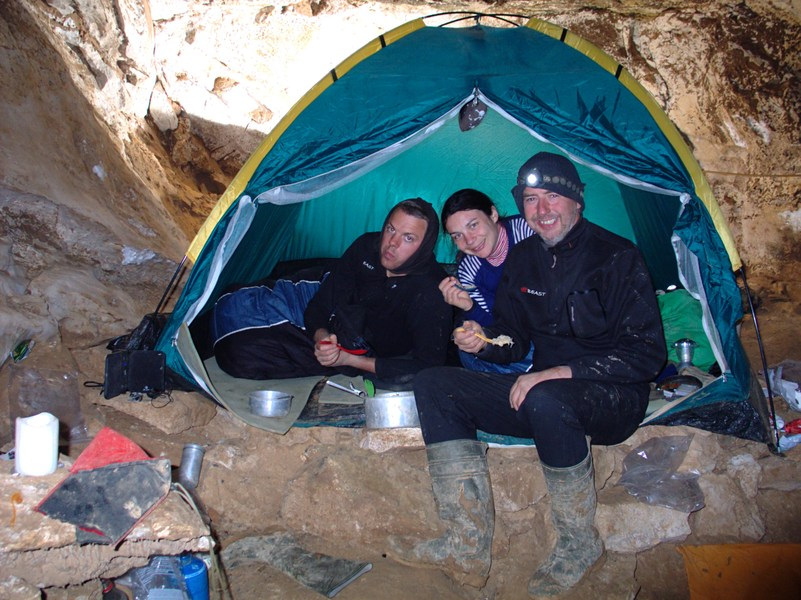
\includegraphics{UgLog1012/22.png}

{[}20100731-23-54-22-Jarvist Frost-Canon G5-CRW\_0405-Camp
\emph{X-Ray}{]}

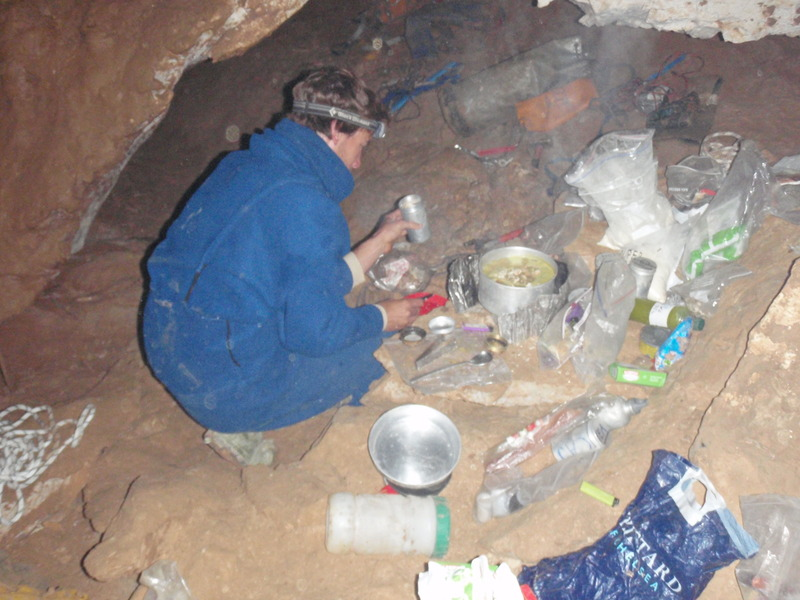
\includegraphics{UgLog1012/23.png}

{[}20100729-13-06-55 - Iztok Mozir - P7294686 - Camp
\emph{X-Ray}{]}\textbf{Izgubljeni Raj 2011} **** \textbf{Revenge of}
\textbf{\emph{X-Ray}}

\includegraphics{UgLog1012/24.jpeg}

{[}The start of 2011\ldots{}{]}

\textbf{21/7/2011 1.45am} \textbf{Jan Clare, Miles, Jarv}

Arrived! 5 hrs down from the sunny plateau with 7 tacklebags, Jarv
(hero) rigged from Space Odyssey. Jan was pursued by a strange chicken
smell which turned out to be a split packet of Bachelors Chicken Savoury
rice. Jarv (weirdo) arrived at camp first (\textasciitilde{}11.30pm)
imagining he'd find an emancipated caver\ldots{} instead there was a
carpet of mould growing on the debris of 2010. We spread sand on the
mold, broke out the comf. collected water, cooked food, set up the fairy
lights and cranked up the tunes! Aah yeah. Tomorrow we hope to recce
\emph{Serpentine}, limit of explo.

\textbf{10:20} \textbf{am} \textbf{Jarv}

Time to get up! reset my 9am alarm so we had a bit more of a snooze (the
Blackadder went off @ 2:30 am). Jan's bladder has dragged us out of bed
-- quite a tight callout, 10PM, so little time to explore.

\textbf{11:07 am (21-7-11) Clare}

Jan is cooking soupy cheesy smash while Jarv and Myles are lazing in bed
listening to Blackadder. I was dragged out of bed by my bladder but
since we didn't have a piss BDH I did a Tetley special and pissed into a
resealable bag instead. Dribbled over pants a bit but otherwise OK. Camp
is super comfy and I don't want to leave.

\textbf{11:22} \textbf{am} \textbf{Myles}

The morning after the night before. Awoke after slightly disturbed sleep
and thus forced to remain in my comf as long as poss. Clare pissed in a
bag, Jan cooked orange smash and we all listened to Blackadder. Camp is
5.3°C! Possible due to the biological processes of the mould
civilisation controlling camp. Now for a little bimble and then out for
tea and medals. WOOF WOOF.

\textbf{12:45pm 21-7-11 Clare}

Myles and Clare. Gone for a little bimble around Leopard. Aim to be out
for sunset. MP3 player died, think its out of battery. See you up top!
{[}Note by Jarv -- charge it with the speaker USB-battery thingy!{]}

\textbf{5pm 21-7-11 Jarv}

Saw Clare and Myles down Albert Hall/\emph{Serpentine}. Sniffed lots of
leads out with Jan:

1 Just after traverse on Consort Road (red rope). Dry oxbow on right
passage (narrow rift) goes back but doesn't intersect passage. Echo
suggests pitch/chamber. Good lead for small fresher.

2 Near Esoterica, waterfall inlet on left. Climb down between boulders
(easiest is to continue towards Albert Hall down mud slope climb then
double back into crawl), follow water sounds to undropped 10-15m pitch.

3 \emph{Serpentine}/It will Rain. Follow red rope down from Albert Hall
-- at end of It will rain, fairly difficult 1.5m cascade/freeclimb to
start of pitch. We rigged \textasciitilde{}5m to ledge, look down 10-15m
(nice pitch!) into what appears to be chamber (big ish). With water.
Left \textasciitilde{}25m 10mm in tacklesack, also \textasciitilde{}12m
10mm left @ end of It will rain.

Reheated tea and peanuts, time to head for surface!

Good luck team Thursday/Friday!

\textbf{22-07-2011 7:45 pm Tetley}

Johnny and Tetley arrived at \emph{X-Ray} after a smooth 4hr journey
down. It's good to be back! Fairy lights\ldots{} not so sure about
them\ldots{} Cup of tea then off for a tourist trip down Friendship
Gallery.

9:45 pm Arrived back from F. Gallery bimble to see Fairy lights\ldots{}
Ah\ldots{} already I associate them with all that's good about u/g camp!
Soupy cheesy fishy smash for supper.

\textbf{22.07.2011} \textbf{Not} \textbf{sure what time\ldots{}. Jonny}

First night at U.G. Camp! had a nice 4hr trip down to camp followed by a
quick trip to the Top of \emph{Big Rock Candy Mountain}. Tasty dinner of
cheesy soupy fishy smash. Lieing in a sleeping bag watching Blackadder
whilst Tetley tries to make \emph{Zimmer} nice. Camp appears to be
comfier than bivi! Looking forward to starting pushing tomorrow.

\textbf{23-07-11 2a.m. Tetley}

Yep left Johnny in camp to play on \emph{Zimmer} for 3hrs, hopefully the
new rig is better. Returned to find Johnny almost asleep. Listening to
some Bach. Sleeping pills for Jonny, Žganje for me!

``For us going to the toilet is a mundane activity, for you it is the
basis of an entire culture'' -- the Red baron (Blackadder).

\textbf{23-07-11 Tetley}

Woke up 10:15a.m. Setting off to push leads beyond Leopard 12:30p.m.
Discoveries await\ldots{}

\textbf{23.07/11 22:00 Jonny}

Just back from a nice pushing trip. Myself and Tetley headed to
\emph{Wonderland} -- hidden surprise, then kamikaze. After a short
hammer to make a squeeze bigger for me we followed a path next to
kamikaze and ended up in a larger chamber `The Red baron' (see previous
page). We surveyed the area; promising lead, traverse across
\textasciitilde{}5m drop. Left the lead to check the end of kamikaze.
Turned out to be a ``COLLECTOR'S PIECE'' (Tet) i.e.~a crawl. End was
blocked although sound of RUSHING WATER was very clear and a passage
could be seen through boulder -- exciting. Trip back was a bit arduous;
dehydrated. Made it back to camp for a great pint of tea, blackadder and
the roar of \emph{Zimmer}. Storm possible up top? Still -- interesting
leas, possibly a horizontal continuation? Making food -- nice cous cous
and sausage.

\textbf{23:00 23-07-2011 Tetley}

Top tip \#1 Don't take Žganje and then take sleeping tablets.

Top tip \#2 If you go to push the exciting lead off Red Baron, take some
water with you to drink!

75m surveyed today, most in `Red Baron', a big chamber. Many thanks to
DW and JKP for leaving us the storming and draughting lead, complete
with a PSS at the start!

\includegraphics{UgLog1012/25.jpeg}

{[}Tetley's sketch of Red Baron chamber{]}

The lead: rope traverse needed over 5?m drop, horizontal passage awaits!

\textbf{23:58 23/7/2011 Tetley}

Went to empty piss BDH -- still a lot of water coming down
\emph{Zimmer}.

\textbf{9:45 am 21/7/2011 Tetley}

A good night's sleep, no headache this morning. Tea and Dangerous Dick.
\emph{Zimmer} is still very wet -- no other cavers have come to join
Jonny and me. I'm in a great mood, Jonny is perhaps apprehensive about
the climb out.

10:30 a.m. We've decided that \emph{Zimmer} is too wet to start
out\ldots{} so we'll be staying warm and dry at Camp \emph{X-Ray} for a
while. The bad news is that I'll have to take a shit. grrr.

\textbf{10.33 am? 27/7/2011} \textbf{Jonny}

Avoiding going up \emph{Zimmer}, flood pulse? Staying at underground
camp listening to music until a reasonable time to get out. May do some
bolting practice? here's hoping that \emph{Zimmer} decides to dry up a
little sooner rather than later

\textbf{24/7 14:45 Tetley}

It's still bucketing down \emph{Zimmer}! Jonny and I are still alone,
Jonny has now broken through the 48hr barrier. We've moved to half sugar
rations, oh life is tough!

\textbf{24.7.11 16:15 Jonny}

Amazing what putting in a single bolt can do. Moral boosted slightly
after contracting a bit of `the fear' and speaking to Tetley about
stories of broken pelvis', rescues and general caving deaths.
\emph{Zimmer} still pissing down so we'll wait until morning before
making ascent, be it wet or not.

\includegraphics{UgLog1012/26.jpeg}

{[}Small cartoon by Jonny showing a wet pitch{]}

More interestingly, seems like the stream near camp \emph{X-Ray} is
likely to be separate

from the \emph{Zimmer} -- water seems to come from opposite direction
(Obviously due to large amount of water). ``Now don't tell me I've
nothing to do''

\textbf{24/7/11 18:20 Tetley}

After an hour of `Dead Ringers' we've moved on to `Little
Britain'\ldots{}

21:25 Jonny and I have both been dozing, still no sign of other cavers,
what's going on `up top'???

23:30 Clare and Jarv arrived at 10:40pm with tales of apocalyptic horror
on the surface -- snow! storms etc. Looks like Jonny and I made a good
call!

23:38 Clare and Jarv gone to push lead off Red Baron -- back to sleep
for Jonny and me.

\textbf{25.7.11 9am} \textbf{Jonny}

C+J arrived back around 7:30am having found \textasciitilde{}200m of
cave. Tetley and myself now off to the surface. Little apprehensive to
leave the comfort of camp but after three nights it's time to leave!

\textbf{25/7/2011 9:05 a.m. Tetley}

Final faff/fag before heading out. Many thanks Jonny for an excellent,
productive, fun 3 night camp -- looking forward to the Laško I left at
the entrance

p.s. Thanks to all who've made \emph{X-Ray} so pleasant -- Jarv
especially.

\textbf{25-7-11 10pm Clare}

Clare and Jarv. Arrived at camp yesterday night and left immediately to
push Red Baron after a chat with Tetley and Jonny. Found
\textasciitilde{}220m of passage we named `The Throne Room' on an 8hr
bolt pushing trip. New Uneo finally worked under Jarv's loving touch!
Night train is hard work though -- caving on autopilot on return to
camp. Now in bed listening to Blackadder over coffee and ready munch.
Jan and Kate, Dan and Myles were supposed to have arrived on the day
train a few hours ago to kick us out of bed but no sign of them. Where
have all the cavers gone?

\textbf{25-7-11 10:30pm Jarv}

Jan and Kate arrive! Nice to see some other peeps. Strange condensation
on the sleeping bag -- perhaps we can dehumidify the whole tent with
carbide?

Mornings in UG camp are a perpetual Sunday Morning. We had chocolate and
latte in bed. It was rather nice.

I think I slept 8AM -- 8PM ish, with a little break for a piss and a sip
of water. Clare was making little sleepy noises, like a rabbit, but
apparently slept little.

The drill is much fun, v quick and efficient.

\includegraphics{UgLog1012/27.jpeg}

{[}Little cartoon by Jarv of him and Clare bolting{]}

Place 8 rawl bolts with the tiny 10-cell Nimh battery.

\includegraphics{UgLog1012/28.jpeg}

{[}Jarv's sketch of the Throne Room{]}

Strong draught over traverse, mostly disappears after climb (stations
1-8). Suspect goes into window, about 4-5m above PSS.8 in chamber. Easy
climb but should preferably protect with bolts. Might be easier to
traverse back from .8

\includegraphics{UgLog1012/29.jpeg}

{[}Jarv's sketch plan of the Throne Room{]}

\includegraphics{UgLog1012/30.jpeg}

{[}Jarv's cartoon of Kate and Jan cooking{]}

\textbf{27-7-11 1am} \textbf{Jarv}

Jarv and Clare. Finally off -- to push Round Pond! callout Noon 26-7-11,
should be back earlier to cook some breccy for K \& J. See ya!

\textbf{26-7 Jan}

Arrived after \textasciitilde{}10pm waking Jarv and Clare, who were
happy to see people. Had food and tea, went to bed after Kate danced to
Duran Duran. Jarv and Clare set off to \emph{Serpentine}. Slept well,
woke 9am. Jarv arrived, had tea, Mexican rice + coffee.

\textbf{26-7-11 Noon Jarv}

Ensconced in the comf, watching Kate \& Jan get ready. Today we did
pitches -- pushed round pond → The Long Water. 40 cm straws in first
chamber, way on via boulder choke then pich up water to small 6m pitch.
Follow stream to cascade chamber -- very pretty. Water goes down a
pitch, also climb to b/choke (a bit small for humans) which prob goes to
same pitch. Also, Clare found `Rotten Row', continue past the first
little dried pool with pretty grey sediment into body-sized phreatic
which leads after a few twists to another pitch. You can see 10m down
onto ledge. Big sound of water but no sign of it.

Good stuff! Left tacklesack with \textasciitilde{}50m of 10mm at foot of
2\textsuperscript{nd} pitch, before cascade climb.

\textbf{26-7-11 10pm Jarv}

Woke at six \& couldn't get back to sleep, accepted this reality at 8 \&
got up to warm some vitaminski in time to receive Myles and Mike. Sent
them off in the direction of Kate \& Jan.

\textbf{27-7 10 50 am Jan}

Woke for a piss after a warm nights kip, Kate, Michael + Myles also in
residence at Chateau \emph{X-Ray}. Yesterday I spent 3.5 hrs bolting
across a traverse at \emph{Cheetah}, Kate waited patiently at top.

\includegraphics{UgLog1012/31.jpeg}

{[}Jan's sketch topo of \emph{Cheetah} traverse. {]}

The last thru-bolt only went in halfway, so the Spirit of Elvis was with
me as I scrabbled for a foothold and reached for the lip of the
window\ldots{} and my light shone to the back for the first time, sadly
it wasn't another exhibition Road but the bottom of a cascade. Still an
exciting traverse nonetheless!

We did a tourist trip to Red Baron chamber then back to camp, meeting
Myles and Michael. Watched RARG on the video player with Jarv + Clare +
Kate in a cosy ball of comf.

\textbf{27-7-11 11:30} \textbf{am} \textbf{Myles}

Mike and I arrived last night and after a brief visit to camp, went to
look at Throne Room. Nice cave! When we returned to camp we found 4
comf-covered creatures refusing to leave! I cooked 7.3 Kg of smash for
Mike + I before settling in for bed. I had a ``Goonies'' style dream,
and now Kate is cooking breakfast\ldots{} Hopefully we're off to push
\emph{Serpentine}.

\textbf{Weds 27 July? Kate}

Yo Yo Yo. Jan \& myself are pushing Throne Room, expect to be back by
10, callout 12. Same times for Mike \& Myles who are \emph{Serpentine}
way. Lots of love Kate.

\textbf{27/7/11 Mike}

Mike + Myles. Leisurely start at 1 ish and headed off to
\emph{Serpentine}. Admired the extra pitches dropped since last year and
followed Jarv's directions to Rotten Row. Looked at two pitches and
bolted the easier one with natural back up.

\includegraphics{UgLog1012/32.jpeg}

{[}Small topo by Mike{]}

Water headed on down, small hole + climb on left or follow water (1.5m
drop). Next pitch approx. 30m? -- Didn't descend whole way. Bolt on
floor+ rigged off natural + dropped \textasciitilde{}10m Wet so swung
over and ascended.

\includegraphics{UgLog1012/33.jpeg}

{[}Another small sketch topo by Mike{]}

Derigged all as neither of us were happy with it. 50m of 10mm and
\textasciitilde{}10m of 10mm left at top. Returned to camp 8:30 ish
after quick survey.

\textbf{Thurs 28/7/11 11.15am} \textbf{Jan}

Jan and Kate. Just contemplating heading out. Had a great trip down The
Throne Room yesterday came back to camp to find Myles + Mike in bed
after an equally exciting push down \emph{Serpentine}! Lots happening

We did two climbs in The Throne Room which lead to a storming passage
called `\emph{Amazing Grace}', after Kate played it on the harmonica
while I climbed, thanks Kate! You took my mind off the scariness +
rapture.

\includegraphics{UgLog1012/34.jpeg}

{[}Jan's sketch of \emph{Amazing Grace}{]}

A good draught is going down `\emph{Amazing Grace}'\ldots{} We turned
round at a muddy climb so someone else could enjoy the push too! Go! Go!
Go!

\textbf{24/7/11 Kate} \textbf{{[}Incorrect date!** **{]}}

My hands are extremely fucked so this may be short. Had a wonderful few
days underground. Camp is as lovely as ever. I've even taken to eating
smash which I thought would never happen after the incident with the
sleeping bag last year.

Had two pushing days, the first of which, despite Jan's heroic effort,
was not so successful although we did answer the unanswered potential of
the window off \emph{Cheetah}. Later that day after sitting at the top
of \emph{Cheetah} freezing my bollocks off we went to find the location
of the Red baron and the pushing front where Clare \& Jarv had an
uninvestigated window.

It was on Jam and my second pushing day that we went there. After much
prodding around Jan climbed and bolted a window above the Throne Room.
Meanwhile I played Jan's harmonica. Annoying we found this window led to
a small passage running parallel to the easily accessible passage in
which Jarv had a shit and that these passages connected via a small
crawl. There was however another window as well. Jan climbed and bolted
this one which led to a wide horizontal passage. We excitedly stumbled
up the passage which then turns 90° to a downward slope. Quite nice and
passable with mud resembling bird poo coating the rocks. With time
running short and Jan wanting to leave it open for the next team (this
want I did not share) we stopped at a muddy easy climb. Could see
another 15-20m but after there who knows.

It's wide, it's horizontal and it's blowing so what are you waiting for?
Go discover some motherfucking cave! Leaving now, Love Kate.

\includegraphics{UgLog1012/35.jpeg}

{[}Small cartoon/sketch by Kate{]}

\textbf{27/7/11 Izi}

Izi, Kletnik (nočna ptiča) **** Sva šla plezat okna v Albert Hall in
Minotaur rift ni blo uspeha. Pol sva šla pa v \emph{Serpentine} zlezla
okno in po kratkem rova dobila majhno brezno na dnu po blatnem rovu
naprej do večjega\ldots{} se nadaljuje (kletnk je predebel). Novi del se
kliče: Let na drugi svet

Camp was perfect!

Hope to be back soon.

HVALA ZA USE

\includegraphics{UgLog1012/36.jpeg}

{[}Sketch survey of Let na Drugi Svet{]}

\textbf{29/7/2011 4pm Tetley}

Back again -- smooth sub 2 hr trip down. Good to see Izi + Samo. Off now
to \emph{Amazing Grace}. Tetley and Clare

\textbf{1:25 am 30/7/2011 Tetley}

Clare and I have returned with 260m in the book -- the new find, after
\emph{Amazing Grace} is called the \emph{Magic Dragon}! Gergely + Jana
also here, in bed, Jarv + Dan off pushing -- more tomorrow after sleep!

\textbf{8:30 a.m. 30/7/11 Tetley}

Dan + Jarv have returned, listening to Ella Fitzgerald, reminiscing
about our great day yesterday\ldots{}We rerigged Jan + Kate's
`\emph{Amazing Grace}' climb (see 3 pages back) so now the `abandoned
climb' is connected to serenade PSS7.

\includegraphics{UgLog1012/37.jpeg}

{[}Sketch survey showing cave from Red Baron to the \emph{Magic
Dragon}{]}

\textbf{30-7-11 23:58 Jarv}

Night train Jarv and Dan. Tet \& Clare finally back from pushing below
\emph{Republika} -- starting to get worried. Mike, Z \& Stane passed
during the night -- first at 3pm to drop stuff off \& check in, then at
5pm to say goodbyeee! Stane popped back to take a photo of the tent, and
then off. Nice to see them all, but disturbed sleep.

Yesterday we visited \emph{Magic Dragon} -- nice crystals/quartz.
Degraded rather horiffically after PSS.1 ; we started to bolt the pitch
but the rock was appalling. Broken \& soft, quartzite broke the Spitz
teeth. Got a bolt in \& natural back up, went over the edge in the
horrific muddiness. The obv natural over the edge turned out to be mud.
The whole pitch lip in fact sticky mud \& white cheesecake boulders.
From the position I was in, sliding around with nasty muddy 9mm, I
plumbed the depths -- 15.5m \& then we bowed out. Slow return with cold
SNOOZES on the boulders to not be too early.

00:17 Jana's here! Tales of horrifically muddy pitch leading to massive
pitch.

Tet \& Clare have left `Daydreamer' at a nice lead above a pitch in
stream.

\textbf{01:45 31/7/2011 Tetley}

Another top trip! Clare and I went down to push below \emph{Republika}.
Dropped 3 pitches and a climb, left big lead -- nice 15+ pitch going
down, white rock, nice stream. Surveyed about 75m, PSS at end. DON'T go
there if water levels are high. \emph{X-Ray} → pushing front about 3hrs
ditto for the return journey. It's going, going, going!

p.s. Our new finds below \emph{Insomnia} pitch are called
\emph{Daydreamers}.

\textbf{01:56 31/7/2011 Gergely}

Good pushing trip today with Jana at the end of the \emph{Magic Dragon}!
We named the pitch `\emph{Stuck in Paradise}', referring to the muddy
awkward terrible nature of it. At the bottom there are two ways on, one
pitch is dead while the other drops to something big, big wind and echo.
It gonna be hard to push though because all you SRT kit is just a big
lump of mud! It will be fun\ldots{} Nice new extensions, big sizes,
crystals and so on. Good to be back. I wouldn't have thought last year
that \emph{Wonderland} will lead to such big things! To the new
extensions, Gergely.

\textbf{29.7 -- 31.7 2011 Jana}

Jana + Gergely. Started late from the surface, we only had like 4hr
pushing. We pushed a small -- on the right bottom -- first chamber at
the beginning of Prince Albert Hall. Small passage went for about
\textasciitilde{}30m. Did a small climb and looks it goes on. Climb not
safe to check. Overall not a massive great lead. After we went to
\emph{Serpentine}, where we checked Samo + Izzy's push. Also de-rig the
original rope at the beginning of \emph{Serpentine} as it got fucked.

Back at camp and soon Clare + Tet joined, followed by Jarv + Dan (night
train). \emph{Amazing Grace} goes and pushed to the \emph{Magic Dragon}.
Clare and Tet stopped at a \textasciitilde{}15m pitch, which Jarv + Dan
decided to push. Sleeping time!

Woken up by Jarv + Dan, muttering about a muddy, horrid pitch. They
could not descent due to mud and then run out of time to bolt around.

Gergely and I decided to push it plus see all the new stuff. Clare + Tet
went to push \emph{Insomnia}. \emph{Amazing Grace} + \emph{Magic Dragon}
is super pretty. Loads of crystals again. The pitch to push is super
muddy indeed. having a drill made job a bit easier and Gergely did a
great job. At the bottom pitch splits in two by rock bridge. One way
dies (sort of -- a climb?) and other is a big pitch
(\textasciitilde{}50). We named the place ``\emph{Stuck in Paradise}''.
Was so muddy you could not see your kit. Not very pleasant SRT. On the
end was completely covered in mud and looked like one big mud blop. Ha,
ha.

\includegraphics{UgLog1012/38.jpeg}

{[}Sketch survey of \emph{Stuck in Paradise}{]}

\textbf{31/7/11 11:17am Clare}

Amazing two pushing trips with Tetley down \emph{Magic Dragon} and
\emph{Daydreamers} -- \emph{Vrtnarija} is now deeper than ever before!
Put in my first bolts and properly dropped first pitches; cheers Tet for
an incredible camping trip and great company. Top tip: hot brews at
-800m is the absolute dogs bollocks. Now all that's left is a final
prusik to the surface. I hope Tetley goes nice and slow! he chased me up
Big Rock yesterday. Till my next camp, happy pushing to all.

\textbf{31/7/2011 Tetley}

So, July draws to a close, as does another great camping trip. Thanks to
Clare, you've been great. Looking forward to sunset and entering
\textsuperscript{1}/\textsubscript{3} km of survey data.

\textbf{31/7/ 18:30 Jana + Gergely}

After a muddy project yesterday, a muddy digging project today, where
again left at the top of the pitch. Great stuff, Jana

Good pushing and have fun. Watch out for the rapture. Gergely

\textbf{31/7/2011 Gergely}

Two digs at Friendship Gallery (don't turn left after the rope, but keep
straight on). Upper one needs explosives; bottom one -- the `Lower
Pleasures' leads to a pitch (cca 20m). Quite good draught, a bit tight
(no SRT kit). Direction \textasciitilde{}210°. To get to \emph{Lower
Pleasures}, climb down between boulders next to the PSS in the last
chamber of Fri. G. It goes slightly towards Sys Mig; but worth giving a
check for the wind also watch out at the end, don't fall down the pitch

\includegraphics{UgLog1012/39.jpeg}

{[}Gergely's small sketch of \emph{Lower Pleasures}{]}

\textbf{1-8-11 Jarv}

Jarv and Dan. What a sleep! From 2pm -- 10:30 am, Wowser. However with
our surface callout in less than 24hrs and us having failed to delay it
we must head out today.

Yesterday we worked on the pitch below Long Water. Didn't much like the
wet way pushed by Myles \& Mike, we went off Rotten Row.

\includegraphics{UgLog1012/40.jpeg}

{[}Jarv's ext elevation of pitch{]}

\includegraphics{UgLog1012/41.jpeg}

{[}Jarv's plan of pitch{]}

Suggestion to keep on rigging is to keep on deviating on left wall, then
bounce to right wall into continuation of rift for the final hang.

The Y-hang gives a perfect hang to the spray lashed ledge -- one could
just throw caution to the wind \& zip down, slam in a bolt in the wet
and continue.

The rotten row PSS 1 was knocked off its corner, I hid the label in the
roof -- it sits on the little ledge on the right about halfway down the
traverse.

\includegraphics{UgLog1012/42.jpeg}

{[}Jarv's small diagram showing location of Rotten Row.1{]}

\textbf{1-8-11 12:40pm Jarv}

Much dead ringers later, and a spot of lunch \& it's time to go. We're
both pretty stiff \& sore -- getting so cold on the wet pitch \& the
caving back to camp clearly isn't good for the body. Water levels still
very low -- I hope someone gets down in time to push \emph{Daydreamers}
and Longwater before it pisses down again!

Excellent clear up operation by the previous two teams -- little left to
take out so we'll tidy up a little, photo inventory \& the elopc (After
some hot vitaminski)

Good luck team August!

Get the bolts \& the metres in!

\textbf{1.8.2011 21\textsuperscript{00}} \textbf{Tjaša}

Grega \& Tjaša. We are going down the stuff (Let na drugi svet?) which
found Samo and Izi. We did some digging and heard a loud water noise.
There was a big draft. We came to water but we had no time to check its
way (we leave it for next day probably). Night!

\textbf{2.8.2011 22:00 Karin}

Nejc \& Karin. We came down around 4:00 had some tea and then we went to
Lower Pleasure. We tried to bolt it but we just couldn't. We came back
and sleep. Nejc is sick so we're going out. There is some rope in Lower
Pleasure left (I think 2 pieces about 10-20m long).

\textbf{3 August 20:30 (morning) Gergely}

Yesterday we went climbing to the Queen's bed chamber. No good luck, the
layers of good rock are separated by muddy layers which are unsuitable
for anything really. Despite the heroic efforts of Izi, he managed to
climb about 7m and came down. We left a rope in for further attempts
(which may involve some mud-stick operation). The window on the left
seems to be going.

Strangle, that now there was no wind at all in the end of Minotaur rift,
although last year it was a huge draught there. The reason may be the
difference in the water level. Today off to \emph{Stuck in Paradise}!
Good luck, Gergely.

\textbf{3 August 2011 Jonny}

Jonny + Dave. Arrived 9 o'clock last night after faffing all day, 3
hours down. Woke at 8 this morning and set off to tackle Big Rock candy
mountain. I sat shivering whilst Dave bolted wind; too muddy, taking too
long, Headed down; nasty rebelay but looks like a large parallel
chamber/shaft! Same dimensions as BRCM. Too late, let someone else climb
up.

Camp super comfy and I feel very comfortable; no rapture

\includegraphics{UgLog1012/43.jpeg}

{[}Jonny's sketch of \emph{Big Rock Candy Mountain}{]}

\textbf{{[}Here ends the original white covered logbook -- all the
following entries are from the red covered supplementary logbook{]}}

\includegraphics{UgLog1012/44.jpeg}

{[}Sketch by Tjaša/Karin showing things to do{]}

\textbf{4.8.2011 9:50am? Jonny}

Jonny and Dave. Fairly restless sleep but here I am, awaiting the
departure to the surface. Despite not discovering much yesterday, it's
been a great trip, especially experiencing some expedition bolting
(cold) and de-rigging (fun). Hopefully I'll be back in the next week,
even if it is for a de-rig. No sign of Izi + Gergely on the night train
-- hopefully they've found something exciting at \emph{Stuck in
Paradise}.

\textbf{5/8 -- 10:30 ish Mike}

Mike + Ari. Have just eaten my body weight in couscous (Dave decline
b/fast) and am both Happy + Sad. Off to go caving down the push on
Friendship Gallery soon.

\textbf{4/8/2011 13:20 Gergely}

Just got back from a good pushing trip with Izi. We found about 500m of
new passage at \emph{Stuck in Paradise}! The rest of the pitch is the
same as the top: a muddy slopy loose-rocky thing. I thought
\emph{Cheetah} was horrible; but now I was glad to come back after
\emph{Stuck in Paradise}. The bolting was fairly OK with some
compromises; the who pitch -- especially the top -- is quite loose, and
it should be 1 person at a time! At the lower bit, the rocks come down
at the clear rock section, watch out.

At the bottom of the pitch a phreatic tube starts. This is similar to
Friendship Gallery in size. Plenty of crystals, very nice walking
passage for about 300m. Then a boulder choke blocks the way, but we
almost managed to climb through in the middle -- there is a crack
between two large boulders which is just too small because of a ledge in
one of them, about 10cm big. This needs a chisel or capping. The passage
seemingly continues on the other side. Watch out for crystals please!

The other passage opens on the left of this one, it is quite low, but
this is the one that sucks the wind. Generally it is about 4m wide, but
filled with mudstone, and not higher than 1m (usually less). We followed
it for about 150m. At the end there is a boulder choke, which seems
passable on the top, but we ran out of time. Strong draught! Crystals
here too and STALAGMITES: about 5 stal columns about 20cm high, 5cm
wide. I think both of these are very good leads, although getting there
takes effort -- this adds to the fun though!

Meanwhile it turns out that we left the instruments \& survey book
somewhere, so tomorrow we have to go back for it. Part of the
fun\ldots{}. Good pushing, Gergely.

ps. The rope in \emph{Stuck in Paradise} is exposed to rockfalls, be
aware!

ps2. The longer passage is called Lost Miles, the windier is
\emph{Penitence}.

\includegraphics{UgLog1012/45.jpeg}

{[}Gergely's \emph{Stuck in Paradise} rigging guide{]}

\includegraphics{UgLog1012/46.jpeg}

{[}Gergely's sketch survey showing extensions below \emph{Stuck in
Paradise}{]}

\textbf{5/8/2011 13:00 Tetley}

Clare and I set off down GW at 9:30am yesterday. Smooth journey down,
meeting Dave + Jonny in Pink. Izi + Gergely were at \emph{X-Ray} with
exciting news of 500m of new cave. ``Do you want to see the book?'' says
Izi. NO BOOK! They left the survey book back in \emph{Magic
Dragon}\ldots{} One for them to sort out, Clare + I were on a mission to
\emph{Daydreamers}. Dropped 3 pitches there, but at the bottom of the
last one the water disappeared down a bedding plane crack\ldots{} Grr,
still I said we'd find a bypass and we did. Left a good drafting lead,
`The Penguin's Egg'. Met Fratnik, Jarv + Jim at Red Cow. Back to
\emph{X-Ray} for some much needed sleep. Thanks again Clare, 140m in
survey book.

\textbf{5/8/11 9am} \textbf{Mike}

Mike + Ari: below `Lower Pleasure', ``2\textsuperscript{nd} Time Lucky''

Went back Fr. am to drop our pitch with correct length rope. Epic faff
on my part which Ari did well to put up with.

\includegraphics{UgLog1012/47.jpeg}

{[}Mike's plan of Lower Pleasure{]}

Two windows down pitch. 5m drop with water at bottom and rift going over
5m drop. Tightish but air fresh -- no draft. Sorry Ari! Happy caving
all.

\textbf{5/8/'11 15:30 Tetley}

Clare + Tetley heading off to \emph{Penitence}, below \emph{Magic
Dragon}

\textbf{6/8/11 Midnight Jarv}

Jarv, Jim, Fratnik. The sun sets on another day train! Karin \& Samo are
already snoozing in bed, we are awaiting the return of Tetley \& Clare
while carrying out experimental cooking research.

Pretty tired and stiff after our long trip yesterday -- we went to find
the Penguin's Egg on our Winter Journey.

\includegraphics{UgLog1012/48.jpeg}

{[}Jarv's sketch survey of Winter Journey{]}

Draft follows squeezes in inclined bedding, eventually wind disappears
into ceiling rift. Heavy silt deposit in lower region of chamber -- near
backing sump? Mud stalagmites on rocks.

\textbf{6/8/2011 9a.m. Karin}

Samo \& Karin. Let na drugi svet -- Krtkova Dobra Dela -- Heroj
Telemarka\ldots{} \ldots{}BAM! Samo fell, so we're going out now. He had
``luck'' that he fell in water. There are 3 leads with water way, 2 up
\& 1 down.

\includegraphics{UgLog1012/49.jpeg}

{[}A sketch survey by Karin{]}

\textbf{6/8/2011 4:20 a.m. Tetley}

Firstly, respect to those, especially Gergely, who pushed Stuck in
Paradise. Amazing push\ldots{} truly heroic etc. Praise to to the
electric drill!

Clare and I went down to push the extensions beneath. We dug through the
boulder choke at the end of \emph{Penitence} to find Salvation -- 200m
of mostly walking horizontal passage. Drafting lead left. Forgot to take
water, despite my own `top tip' early this expo, hence pretty dehydrated
after 10 hrs caving, no water to be found. Grade 1 survey to follow
after sleep. A great day, only marred by news of Samo's injury, I hope
he's OK.

\textbf{6/8/2011 9:45a.m.} \textbf{Tetley}

Note re: \emph{Stuck in Paradise}

Only one person should be on the pitch at a time. It takes 30-40 minutes
to ascend or descend.

If you shout `rope free' at the top, you won't be heard at the bottom
and vice versa\ldots{}\ldots{}.

\textbf{6/8/11 9:50 a.m. Tetley}

Tjaša and Eric here after coming down and pushing on the night train.
Samo, Karin and Fratnik heading out soonish.

\includegraphics{UgLog1012/50.jpeg}

{[}Tetley's sketch of Salvation{]}

\textbf{6/8/2011 1:20 pm Clare}

Another camping trip drawing to a close, quite probably my last pushing
trip of the expo! Just waiting for Jarv and Jim to return before we
start our bid for the surface. Once again, two successful pushing trips
down below \emph{Daydreamers} and in the kamikaze extensions below Stuck
in Paradise. Another 340m in the book, and caving with Tetley's always a
pleasure. Special thanks to Gergely \& Jana \& Izi for bolting and
rigging and surveying the worst pitch in the world (\emph{Stuck in
Paradise}) so beautifully. We left a strong, draughting lead in
Salvation below the pitch, go push it!

\textbf{6/8/2011 13:30 Tetley}

Time soon to head up for tea + medals. Another great trip!

\textbf{6-8-11 22:00 Jarv}

Jarv \& Jim. Another glorious morning down @ Camp \emph{X-Ray}! Well, it
is night but who cares? Only hit the sack @ 16:00, thanks to sliding
forward in sync with Tet \& Clare.

Just had a strange dream for caving -- searching amongst Hipster pubs in
London with Jim; we were looking for other cavers but mainly for
1\textsuperscript{st} class toilet facilities. Here, alas, the piss BDH
is full.

Yesterday we went to the \emph{Serpentine} to try \& drop the wet pitch.
Didn't quite make it -- needed a rebelay \& found a natural but it was
just too dodge for the swing I'd undertaken. Jim was also shivering in a
sleeping bag, where I'd swung too was wet \& NO PLACE TO HAND BOLT.
Perfectly possible to rig this pitch dry, but requires a fair bit of
swinging \& a fist full of bolts.

\includegraphics{UgLog1012/51.jpeg}

{[}Jarv's sketch of `Drink Your Own'{]}

Anyway, having made a stab at it, and grabbed a few quick photos of the
straws in Longwater we withdrew gracefully.

Well, actually that was bollocks as we derigged the whole pitch series
\& found ourselves with three tacklesacks + a bolting kit through the
\emph{Serpentine} meander. Pretty epic, as one was a massive `Big
Bertha' sleeping bag tacklesack stuffed to the brim with wet 10mm \&
metalwork. Still, made it to Friendship for 2pm, having left @ 5am. A
few plates abandoned in-situ, as rawl threads damaged by hammer.

\includegraphics{UgLog1012/52.jpeg}

{[}Jarv's sketch of \emph{Serpentine} pitch rigging part 1{]}

\includegraphics{UgLog1012/53.jpeg}

{[}Jarv's sketch of \emph{Serpentine} pitch rigging part 2{]}

\includegraphics{UgLog1012/54.jpeg}

{[}Jarv's sketch of \emph{Serpentine} pitch rigging part 3{]}

\textbf{6.6.2011 23\textsuperscript{00}} \textbf{Tjaša}

{[}For the next few entries, the recorded month changes, from 8 (August)
to 6 (June)!{]}

Erik \& Tjaša. We are going surving (?) The new parts around Krtkova
Dobra Dela we founded yesterday Kletnk \& Karin and if we will have time
do some pushing there. Lep pozdrav!

\textbf{6-6-11 22:50 Jarv}

Jarv \& Jim. Well, we've had Hippy tea \& a blast on the music player.
The gizmo is recharging \& we're going to try and get a little more
shut-eye before departing.

\textbf{7-6-11 13:00 Jarv}

Well! A bit more shut-eye turned out to be more than anticipated!

Erik \& Tjaša came back very quickly from surveying -- they got cold \&
wet and crawled into bed with us!

A very long sleep but worth it. Jim is feeling a lot less stiff \& my
back is popping less. Certainly the derig yesterday exacted its toll.

Camp is looking rather bare, nil shitbags, meths, sugar, hot choc, rice.
The train is crashing \& it's time to get off.

\textbf{14:48} \textbf{Jarv}

Good luck Erik \& Tjaša, see you on the surface!

\textbf{7.8.2011 17\textsuperscript{00}} \textbf{Tjaša}

We were surveying and get very wet. We had surved Heroj Telemarka that
found Samo \& Karin yesterday. Samo falls into the waterand there is
also our surveying stopped. That is on the left side (part on Karin's
drawing where are ``two amazing lakes''). Then we went to the right.
Karin had written that there are 2 meanders but is only one. It just
looks like there are 2 because they're one above another but after a few
metres they become one. That meander ends after 30 meters. There is
water so we couldn't get over it. I think it is possible but you get all
wet. So we end after 30 meters. We do the last station on a rock wich
looks like this but we didn't put any paper because it hangs from the
cealing (strop -- SLO).

\includegraphics{UgLog1012/55.jpeg}

{[}Tjaša's sketch referred to above{]}

We decided that the name will be the same as Karin \& Samo gave it to
the nearer part and because they told us to go there. So, it's named
Heroj Telemarka.

We eat 2 frutabelas there and go surveying the part which founded I and
Grega few days ago (that little canyon). We named it Krtek in Orel. The
last station is above the bigger pitch. We didn't surved it down because
we didn't want to get wet. Anyway, when we went back + swing on a rope
accidently under the waterfall and get wet. And Erik get wet in the
squeeze in Krtkova Dobra Dela. So, we were all wet in the end.

Shit happens : )

Under the bigger pitch Erik bolted something and it's possible to go
down. If you follow the water you come to a lake and it's impossible to
get there without getting wet (the level of the water is high to knees,
something like that). The possible way going further is above the water.
It's something like passive meander, it needs to be looked one more time
to see if it's possible go further without going into lake.

We're going out today. See you and good luck to everybody!

Now I see that I left 2 pages empty. Ups

Well I can draw something

\includegraphics{UgLog1012/56.jpeg}

\includegraphics{UgLog1012/57.jpeg}

{[}Tjaša's drawing{]}

\textbf{7.8.2011 21\textsuperscript{00}} \textbf{Tjaša}

Erik and Tjaša. As it seems we are staying in camp because there is a
waterfall in Zimer. So, good night

\textbf{8.8.2011 11\textsuperscript{00}} \textbf{Tjaša}

the water calms down slowly but there is still a lot of it in Zimer. We
hope that on the surface cavers don't panic because we won't come out at
the callout.

Today is Erik's mother Maria birthday. It seems that he will miss the
party

\textbf{8.8.2011 14\textsuperscript{00}} \textbf{Tjaša}

Much more water than in the morning.

\textbf{9.8.2011 14\textsuperscript{00}} \textbf{Tjaša}

Finaly! Gergely and Tetly come in camp. It means we can go out.

Thanks for nice \& warm camp! Tjaša \& Erik.

\textbf{9 Aug 2011 13:45 Gergely}

This tear the last time in Camp \emph{X-Ray}! We wanted to come down
with Karin to push Salvation, but the storm put us off. So today we came
in 1.5 hours with Tetley to check if Tjasa and Erik were good, after 24
hours their callout. Luckily, everything is all right and the camp is
rocking with music! Great times! The cave is still wet but it is time to
go. Another year, another expo, another success. See you next year!

To the connection and the new passages and to infinity.

\textbf{9/8/11 Tetley}

Exactly 10 years after the discovery of Friendship Gallery we're packing
up and leaving for another year. A great year -- over 2km of new cave.
Looking forward to returning in the future.

LEFT at X Ray 2011

5x 4.5 Flatcell

6x AAA bats

4x AA bats

1 kg carbide

20+ choc bars

12 tins fish

some nuts/noodles/soup

1 full power gas cylinder

\begin{itemize}
\tightlist
\item
  1/3 full power gas cylinder
\end{itemize}

1 large blizzard bag

1 tent

1 good 30m tape measure

500m + rope

\begin{itemize}
\tightlist
\item
  50m dynamic
\end{itemize}

10 slings

1 pair of Samo's pants

25 spits and cones

40 stainless hangers

15 stainless rawl bolts

\includegraphics{UgLog1012/58.png}

{[}2011-07-31-01.11.35-Jarvist M Frost-CanonA520-IMG\_0167 - Jana and
Tetely Cooking Lond Exposure{]}

\includegraphics{UgLog1012/59.png}

{[}2011-08-01-13.24.46-Jarvist M Frost-CanonA520-IMG\_0175 - Food
Reserves and Stove at Camp \emph{X-Ray}{]}

\includegraphics{UgLog1012/60.png}

{[}2011-08-01-13.24.09-Jarvist M Frost-CanonA520-IMG\_0173 - Dan
Drinking Tea in the Tent at Camp \emph{X-Ray}{]}

\includegraphics{UgLog1012/61.png}

{[}2011-08-03-10.31.54-Grega-Panasonc DMC-FT2-105-camp \emph{X-Ray}{]}

\includegraphics{UgLog1012/62.png}

{[}2011-08-07-12.10.52-Jarvist Frost-CanonG5-CRW\_0178 - jim at camp{]}

{[}Editor's note: Everything in square brackets has been added by
Tetley. I thought it was best to type up the writing; it took a lot
longer than I thought it would when I started but it's been good
reliving the memories! I've tried to keep original spelling etc., but a
few typos may have crept in -- sorry! Scan quality of drawings not the
greatest, again apologies. I added the photos to the document just for
the memories\ldots{}.May 2012{]}

\textbf{Sledi Vetra 2012}

\textbf{11:45 Weds 18/7/2012 Jonny}

Back in underground camp one year later!\\
A smooth trip down, everything has now been de-moulded in camp. Tea
ready, about to cook.. It's good to be back!

\textbf{Niko}

Finally back in camp \emph{X-Ray}, mental! Last time I was here two
years ago. Journey here was generally alrite, just Jonny sort of started
leaving tace sacks as he started rigging, so more load 4 us, but he did
a good job rigging. \emph{Zimmer} annoying. Camp was quite mouldified,
but Jonny covered with sand. Cooking now, everything is alrite.
Definitely less rapture than 2 years ago. I just sort of thought that
it's a pretty unique situation here. Cos normally whatever youre doing
in life (eg smoking weed) there must be a lot of people at that same
instant around the world doing the same thing, but I think at this
moment, we are very likely the only people in this world living in a
deep underground camp, like us. Crazy thought. We are truly alone.
Waiting for cous cous. Everything is alrite. So yea, Camp \emph{X-Ray}
2012 is again in operation. Enjoy!

\textbf{Oli}

Gone down more pitches than I can remember.. Underground camp is
actually much warmer than I thought it would be. Time for dinner --
Ainsley Hariets cous cous.

\textbf{1:47 am Friday 20\textsuperscript{th}} \textbf{July Rhys}

Nice easy trip down to camp. Left at sunset, down for about midnight.
Have eaten cous cous, smash and sausage. I don't know what I thought
camp would be like but I'm here and I like it. Hopefully shall have nice
long sleep.

\textbf{2:30 a.m. 20/7/2012 Tetley}

Back at \emph{X-Ray} -- the 4\textsuperscript{th} year we've had a camp
here ('03, '10, '11, '12). Rhys and I had a smooth journey down -- now
drinking Žganje and listening to Blackadder. Now some sleep!

\textbf{11:40 a.m. 20/7/2012 Tetley}

A decent kip, slight headache though. I'm thinking of tea, and the
pushing front.

\textbf{12:47 p.m. 20/7/2012 Rhys}

Sleeping was good, camp is comfy. Breakfast soon, yum. Really excited
about pushing. Where else can you doss about in the sun one day and be
at the limit of human exploration the next day? Its going to be good.

\textbf{2:40 p.m. 20/7 Tetley}

The classic `Cheesy, soupy, fishy smash' for breakfast. Almost finished
packing food, brew kit, bolting kit, rigging kit, survey kit. Had a
shit. Cup of tea then time to put caving kit on\ldots{}.

\textbf{Tet}

It's 20⁰ Celcius down here -- or so says the thermometer I bought in
Tolmin! Dr.~Tim, a rubber chicken (and Samo's pants!) are watching over
us!

``It's not just about the pushing, it's also about the journey.''

``Yeh''

\textbf{3:50 pm 20/7 Tet}

Rhys and I are finally heading off to Salvation. Back by 8 a.m. at the
latest.

\textbf{4:10 pm 20/7 Clare}

Good trip down with Jarv, great to be back at \emph{X-Ray}! Nothing's
changed, it's like coming home. Had a quick chat with Tet and Rhys just
as they were leaving to push Salvation. We will be off to kill Winters
Journey and derig the \emph{Insomnia}/\emph{Daydreamers} series. May
also check out Red Cow and Strap in the Nitro. Expect to be back 9am on
21/7, callout noon.

\textbf{4:15 pm Jarv}

Great to be back! Off to kill the deep stuff.

\textbf{21-7-12 6} \textbf{AM} \textbf{Jarv}

Back!

Pushed: PERFIDIA, a tight dry alternative to \emph{Republika} (pitch).
We were hoping for a Red-Cow sump bypass.

Then went to the bottom \& pushed WATERSHIP DOWN from beyond
WinterJourney.1 (where Fratnik \& Jim opted not to squeeze) down a
{[}STUPIDLY{]} freeclimbed slope to a beautiful deep static sump.

The cave is thus deeper -- perhaps 20-30m so.

\includegraphics{UgLog1012/63.jpeg}\\
{[}Jarv's sketch of Watership Down{]}

Most is steeply inclined bedding.

Sump (or Lake?) has no water flowing into it. Crystal clear \& could be
percolation water. Obvious windows above sump/lake that could be gained
by traverse from slope-pitch.

\textbf{21/7/2012 10:10 a.m. Tetley}

Rhys and I are back from a 17 hr pushing trip - ≈100m in the book. Cave
beyond Salvation named Brave **** New **** World. Clare + Jarv in bed,
we'll soon be joining them in the tent -- more tomorrow. Thanks Rhys for
a great trip!

\textbf{21/7/2012 6:57 pm Clare}

Jarv and Rhys are asleep on either side of me, Tetley smoking a fag in a
corner of the tent -- all is well at Camp \emph{X-Ray}! Excellent push
yesterday, even if everything we found (\textasciitilde{}150m total?)
seemed to be body-sized or smaller!

PERFIDIA is a cool connection between Red Cow (pitch rope) and the start
of \emph{Insomnia}. Saves a fair bit of time, though only go there if
you aren't carrying lots of tackle and are shorter than Jarv!

Tried to kill Winter Journey but it won't die. Amazing that there is so
much cave off an abandoned bedding plane that Tet and I explored out of
desperation last year! We found a series of rabbit warrens -- little
crawlways at a bedding plane incline. Named it WATERSHIP DOWN. At the
end of it is a gorgeous terminal sump (or lake?). Named it MALA BOHIN
(?? Whatever that famous lake is called). Still a few unexplored leads
in Watership down, including what looks like a pitch. Take some rope.
There is loads at Red Cow Roundabout, and a length or two at the start
of Penguin's Egg. If you want to get down to the sump, I'd recommend
rigging a rope down the final slope -- I'd have been stuck there if not
for Jarv to stand on!

Right, going to try and grab more shut eye.

\textbf{11:36 pm 21/7/2012 Rhys}

Just woke up from 12 hour sleep, feeling good. Camp is nicer with 4
people. Tea now, hopefully breakfast soon. Selective memory has already
turned yesterday from mostly slogging through \emph{Penitence} and Stuck
in Paradise to an amazing trip.

At end of Salvation we (mostly Tetley) hammered our way through squeeze
to cool chamber and then Tetley entombed himself digging into boulder
choke. This eventually led to weird streamway. Very drafty all the way!
Definatley two leads up and down streamway. New discoveries called Brave
New World. Looking forward to going back.

\textbf{21-7-12 11:47 PM (says my watch -- feels like 10 AM) Jarv}

Fairly cool night (buf + a fleece liner with an irritating feet-sized
hole in the bottom. Legs kept on cramping -- it's a lot of exercise to
the new new bottom of the cave.

No nightmares about not being able to climb back up from Watership
Down.1 In fact I didn't dream much at all. Just daydreamed of the
beautiful sump \& the crystal clear water.

You wake after a push \& rub the mudstone-sleep out of your eyes, sore
knees, stiff muscles \& odd bruises in strange places. Hmm, anyway --
back to the cave.

Perfidia, the attempted Mad Cow Sump Bypass

\includegraphics{UgLog1012/64.jpeg}\\
{[}Jarv's sketch of Perfidia{]}

I hate \emph{Republika} \& \emph{Insomnia} (pitches). Both are wet,
perversely rigged \& make me very unhappy on return from the deep. In a
sane world both would be rerigged -- but this would require time, bolts
\& new rope. Thus unlikely to happen unless a serious effort is made on
the sumps.

\emph{Daydreamers} rope was actually all OK -- inspite of being left
rigged last summer. \emph{Insomnia} I had to reverse prussic as it had
been tied off (I suspect) by the last climber last year.

Maillons in Dreamers were v.rusty but not structurally so.

Ends of rope where cut had been pulped. The swing-pitch above the pool
had extreme rope rub on where the horizontal section had been
tap-tapping on the floor. Ropes were pulled up \& tied off were
possible.

\includegraphics{UgLog1012/65.jpeg}Rope:

\begin{itemize}
\tightlist
\item
  1 x 10m, 15m, 20m 9mm @ Red Cow (taken from \emph{X-Ray} on this trip)
  + unknown-length old 9mm
\item
  ̴20m excess 9mm on Red-cow Y-hang
\item
  ̴10m excess @ end of \emph{Insomnia}
\item
  ̴20m new 9mm \& ̴15m old 9mm @ Penguin's Egg
\end{itemize}

Big Rock -- hangers were rather corroded. Didn't like it much --
substitute soon? All bolts were very loose -- does someone come \&
loosen them over winter? Odd.

Left a few dirn. arrows for Red Cow \& back to Big Rock (as far as
Leprecaun pitch) Not sure if they help much, but we do try\ldots{}

{[}Jarv's sketch of sump chamber{]}

\textbf{22-7-12 1:24} \textbf{AM} \textbf{Clare, Rhys, Tetley \& Jarv}

HAPPY BIRTHDAY PETE!

\textbf{22/7 2:18} \textbf{am} \textbf{Tetley}

3 pages are missing from the back of this logbook\ldots{}. The first
team down forgot to bring toilet paper. Apparently the paper I'm writing
on is soft, strong and thoroughly absorbent! The camp setup team* did a
great job though, \emph{X-Ray} is as homely as ever, too nice at the
moment to make me want to put my furry on too soon.

{[}*Jonny, Mike, Olly and Nico{]}

Great trip yesterday, we had hot tea and cake at end of Salvation.
Digging and hammering for 40 mins, and I just got through the squeeze
left at the end of last year's expo.

Back in new territory. More digging and hammering enlarged the squeeze.
Rhys and I were now in a small chamber. Wind so loud through squeeze it
sounds like the roar of a stream.

Damn, no way on, big boulder choke. Wait\ldots{} maybe up there,
no\ldots{} yes\ldots{} hanging death above. Tried to dig up but scary
boulder led to a change of tactics, went right, horizontal, under said
boulder. Scary digging up, but I had the draught and could see big
passage above\ldots{}.

Soon I had a hole large enough to squeeze through. Told Rhys to smoke
all my tobacco if I should die and went for it. Crash. Collapse, I was
trapped. Well past the point where rescue is possible\ldots{} Could just
move left hand\ldots{} slowly, with the help of Rhys, I dug myself out
and we were through.

Its true to say that we weren't in the huge, horizontal passage with
stals and gour pools that I'd dreamed about. But it didn't matter! The
thrill of being in new, unexplored passage never wears off.

Up a slope (crawling) passage gets bigger heading east going up at ≈40⁰
to horizontal. We climbed up a slope until passage broke into what looks
like an active streamway (though it only has a tiny trickle of water in
it -- not even enough to collect to drink). Upstream left unpushed,
downstream has the draught! We surveyed ≈20m down stream. Left
draughting bedding plane crawl as the going lead.

\includegraphics{UgLog1012/66.jpeg}{[}Tetley's sketch of \emph{Brave New
World}{]}

\textbf{22/7/2012 5:20 am Clare}

Clare + Jarv off to push Throne Room. Expect to be back by 2pm.

\textbf{22/7/12 6 a.m. Tetley + Rhys}

We've found Xanadu!

\includegraphics{UgLog1012/67.jpeg}\\
{[}Tetley's directions to Xanadu{]}

\textbf{22/7/12 noon Rhys + Tetley}

Back from Xanadu for tea (a pushing front 5 minutes from camp is
great!). It goes! Theres a deep narrow rift with a stream at the bottom.
We descended right down to the stream and followed it down to a sump and
followed it up to an impassable waterfall. At higher levels in the rift
we may have found a sump bypass (going to explore that now) and there
may be a waterfall bypass but we haven't looked. Great trip so far!

\textbf{22/7/12 14:00 hrs Clare}

\includegraphics{UgLog1012/68.jpeg}Just back from Throme Room with Jarv;
he's having a shit, water for cous cous is heating up, Night of the
Proms on stereo -- another day at \emph{X-Ray}!

Exciting stuff from Rhys and Tet above! They aren't back yet, Xanadu
must be going in a big way. And so the leads keep multiplying\ldots{}.
Jarv and I returned from Throne Room with two new leads: a pitch and a
sandy crawl -- both draughting. About 50m more in the book after Jarv
bolted across the pitch at the end of Throne Room and up a slippery
slope. The pitch goes, and at the end of the slope you get to chamber
with a sandy crawlway. Our new finds are called HOT PANTS (``I've a
plan, and it's as hot as my pants!''), after Jarv had another shit in
the Throne Room.

{[}Clare's sketch of Hot Pants{]}

\textbf{22/7/2012 14:38 Jarv}

Mmm, oil-less couscous. It's been a while.

The Uneo proved its worth again attacking the two `sort of leads' we
left at the end of the Throne room.

Pitch) Easily dropped with bolt on large boulder \& tackle-bag rub
protected descent. Crawl opposite lead immediately to
\textasciitilde{}4m draughting (sucking in) pitch. Possibly free
climbable. Definitely goes somewhere, I returned up to attend the
traverse.

Traverse) Horrific to bolt. Rock v. dodge. All foot holds loose/dubious.
So much shit came down/on me. I found myself unintentionally landing on
my cows-tails more than once, and once a day is quite enough.

Traverse proceeds up 60⁰ inclined slope of death. Minimally gardened to
avoid slicing rope. Top section is a jammer/abseil section that goes
over a massive pile of boulders, extreme care \& possibly a rebelay bolt
required.

From top of traverse (phew!) careful climb up slope \& through boulder
choke to a fairly impressive chamber \textasciitilde{}7+m high with
passage leading of at about \textasciitilde{}4m above floor.

More importantly, a crawl goes from the edge of the chamber blowing into
your face over a white mud/stone blockage that is easily diggable (Clare
just slipped over). Apparently it continues on \& on. Perhaps ideal for
the small wrigglers amongst us.

\includegraphics{UgLog1012/69.jpeg}\\
{[}Jarv's Hot Pants Rigging Schematic{]}

\includegraphics{UgLog1012/70.jpeg}\\
{[}Jarv's sketch of Hot Pants chamber{]}

\textbf{22/7/12 3:00 pm Rhys}

The sump bypass goes! Its got a big draught. It's a muddy crawl with a
puddle that proved too much of a psychological barrier to pass so we
left it as a good lead. To get there go to Xanadu and down to the top of
the rift, descend using the red rope as a safety rope/handline to the
rift level with the Y-hang, then head downstream on that level (no leads
down y-hang). T'was a good trip.

\textbf{22/7/2012 4:40 pm Tetley}

Another great pushing trip. Xanadu is an interesting rift, with
different levels. Made our way down to stream level ≈30m below
Friendship Gallery. Upstream goes to a wet squeeze, downstream to a
sump. Pretty white rock, lovely ripples on pool of water, found what we
think is a sump bypass. Two possible leads --

\begin{enumerate}
\def\labelenumi{\arabic{enumi}.}
\tightlist
\item
  Push up high up stream
\item
  The strongly draughting muddy tube with puddle (sump bypass?) --
  sketch to follow later
\end{enumerate}

Interesting surveying, Rhys did book for half of our 18 or so legs. ≈90m
new cave found. A great change from last pushing trip to have
\emph{X-Ray} 10 mins from pushing front. Now in bed, listening to `the
Ascent of Run Doodle'.

\textbf{22/7 8:50 pm Tetley}

3 hours of (Žganje induced?) sleep and I'm awake again. No sign of a day
train\ldots{}. One would be good on the deep pushing front but bad for
me, don't want to get kicked out of bed. On Saturday the stream sounded
pretty loud (but not of the apocalyptic level Jonny and I heard last
year. Now it sounds fairly normal.

\textbf{22/7/12 9:01 pm Clare}

Really should be asleep, but am just on the wrong side of restless to do
so! Fingers crossed the day train doesn't arrive to kick us out of
bed\ldots{} Rhys has just got up for a piss, only to find the piss BDH
full\ldots{} so he promptly went to \emph{Zimmer} to empty it. What a
trooper!

\textbf{23/7/12 1:22 am Rhys}

Sam and Mike have arrived looking for beds. Tetley has used jedi mind
tricks and convinced Clare and Jarv to leave now. More sleep for us then
out I think. I wish I could stay and push more but the surface and
dossing calls.

\textbf{23-7-12 1:34} \textbf{AM} \textbf{Jarv}

Oh no! They're here\ldots{}. Mike \& Sam arrive, in search of comfort
form the storm.

\includegraphics{UgLog1012/71.jpeg}\\
{[}Jarv's drawing of his chafed legs{]}

Note to self: Wear leggings to avoid pain

As I'm rather suffering from the waste-down \& it would be rude to push
the near-camp leads \& not looking forward to a long painful traverse to
a worthy pushing front, it makes sense for Clare \& I to leave early \&
give Rhys a little more rest before heading out.

\includegraphics{UgLog1012/72.jpeg}\\
{[}Tetley's extended elevation sketch of Xanadu{]}

\textbf{23/7/2012 3:30 a.m. Tetley}

A strange very broken night\ldots{}. Jarv + Clare are now getting
changed ready to go out (Blondie playing quietly). Mike + Sam in
sleeping bags, together with Rhys + myself. Jarv drilling with electric
drill\ldots{}.. (to make extra clothes rail).

\textbf{23/7/2012 3:30 am Clare}

Alas, Mike + Sam came down on the day train around midnight, just as we
thought we were going to have another 8 hrs in bed\ldots{} Oh well,
guess we have to hit the surface sometime. Will be good to see the sun
again. It's been a great camping trip, cheers Jarv! And Tet + Rhys for
making \emph{X-Ray} fun. Excited to enter our survey data! Will be back
soon to push more leads, good luck team 2012!

\textbf{Tetley}

Some thoughts on pushing beyond \emph{Brave New World}

\begin{itemize}
\tightlist
\item
  It's a very serious trip -- don't underestimate it, even a club rescue
  might not be feasible, a major injury would be a disaster best to
  think RESCUE IMPOSSIBLE
\item
  Take Water. Rhys + I took 1.5 litres each, this was about right. No
  water in cave from \emph{Zimmer} onwards.
\item
  Recommended: a brew kit, (meths + fish tin). Hot tea and hot fish
  sandwiches went down a treat!
\item
  Allow a minimum of 4.5 hrs each way between \emph{X-Ray} and the
  pushing front.
\item
  \emph{Stuck in Paradise} -- Rhys + I went down and up in sections, one
  at a time, i.e.~I went down to a point where I was safe from falling
  rocks then stayed at rebelay until Rhys joined me, we then repeated
  this. This worked very well!
\item
  On two sections on way down rope had caught around rock/flake so was
  very taut. Down prussiked/Italian hitched down.
\item
  ≈20m of yellow rope is at top of Stuck in P.
\item
  ≈40m of rope has been left at end of Salvation.
\item
  Rhys and I had a 17 hr trip.
\item
  Some draught from \emph{Amazing Grace} all the way through to Brave
  New World pushing front. What's driving it????
\end{itemize}

\textbf{23-7-12 03:52 Jarv}

So long \emph{X-Ray}!\\
Another fine 60 hour stay (check-in till check-out).\\
Some great pushing, we've left some good leads -- just treat the Throne
Room traverse \& new deep bits with respect -- they're not as protected
as should be \& rescue from both would be difficult if not improbable.

Off with the camp rubbish \& flat drill batteries, and a too-exciting
mix of methanol \& petrol (that first day in the Bivi mix up still
haunting us).

Safe caving, good luck pushing \& see you again as soon as my sores
heal!

\textbf{23/7/12 9:45 a.m. Tetley}

Rhys and I left the surface 85 hrs ago. Rhys throughout has seemed
utterly unfazed by his first camp, deepest trip, longest days pushing,
caving with me (!) etc. etc\ldots{}. Mike snoring on and off, Rhys + Sam
lying silently in pits. I'm fully awake now, listening to Bach (and
Mike's nose) and drinking tea. This cave and the cavers who push are
truly amazing, the combination of the two is something very special
indeed! It's strange, normally after this much time underground I'm very
keen to see the sun; on this trip, however, I haven't really even
thought about it. Is this a good thing or a bad thing???

\textbf{23/7/12 10:24 am Rhys}

Weird 19 hours in bed, was awake for about 9 hours of it I think. Tetley
making tea. Inevitable trip to surface rolls closer.

\textbf{23/7/12 10:30 am Sam}

Don't think I got a great deal of sleep last night. I was plenty warm
enough\ldots{} but it was difficult to drop off. Perhaps because of
Mike's snoring? Anyway camp is a pretty cool place, and I don't feel
quite as weirded out as I thought I would be. Trip down was ok, but
long, because I got caught up on the last couple of pitches. Up to then,
everything was fine, and motivation was high. Enthusiasm did start to
flag\ldots{} until camp was reached. I like it here\ldots{}

\textbf{23/7/12 12:50 pm Rhys}

Finally kitted up and heading out. It's been an epic experience and I'm
looking forward to coming back, perhaps to push \emph{Brave New World}.

\textbf{23/7/12 1 p.m. Tetley}

A great trip -- thanks Rhys! Beer (and hopefully good weather) up top.
Happy cave hunting everyone!

\textbf{23/7/12 13:30 Mike}

Breakfast followed closely by lunch with the Flaming Lips providing a
`spaced-out' soundtrack; Nice to be back in camp, my best nights sleep
in \emph{X-Ray} as witnessed by my proud snoring! (Just prod me\ldots{})

Off for two gentle pushing trips this afternoon (I didn't think SAM or I
want more at the moment) but it feels good to be surrounded by
Tetley/Jarv's enthuasism and successes, hopefully we can provide more
answers to this Mountains mysteries!

→ \emph{Lower Pleasures} (check bottom pitch, Avens ok)

→ Xanadu: check higher rifts etc

Back at Camp by 10pm

\textbf{23/7 20:00 Mike}

Back form a simple pushing trip with a few positive leads found at Lower
Pleasures.

Worth another trip see overleaf for two avens that are going leads.

\includegraphics{UgLog1012/73.jpeg}\\
{[}Mike's sketch of leads at \emph{Lower Pleasures}{]}

\textbf{23/07/12 20:05 Sam}

Mike and I just got back from our trip. Although not particularly
successful, as the first trip of its kind for me it was hugely valuable.
We first headed off for \emph{Lower Pleasures}. Getting there was smooth
enough except a fair amount of time was spent removing a boulder from
one of the crawls. Once at the bottom, I poked my head around the
potential lead. Sloping up to the right was too tight; the only possible
way was ahead through a small rift with water at the bottom. (wet rift
streamway). Although I got a little way, the streamway narrowed so that
to continue one would have to be on their side, lying in water. Further
on, there was a very sharp corner which made it even more implausable to
try and pass. So, my first lead and a dead end! I then went up the first
rope and waited while Mike checked out another couple of leads, in a
couple of avens. Apparently these are promising leads, along with a
third aven which is harder to get to.

We then on our way back had a look around Xanadu. Nothing more was found
but it was fun to root around in such recently discovered passages. So,
I enjoyed the trip. It was short and relatively simple, which I
definitely required. I'm beginning to realise that I have a long way to
go before I can consider more serious trips. But these past couple of
days have been an amazing experience, and maybe one day I'll be able to
come back. Camp is still awesome. Hopefully tonight I'll sleep better
than last night, especially for getting to the surface tomorrow\ldots{}

\textbf{24/7/12 Sam}

Second night at underground camp was better\ldots{} I got a lot more
sleep. Looking forward to being back on the surface, despite feeling so
immensely confortable down here right now.

\textbf{24/7/12 Mike}

Also had a quick look in Xanadu yesterday; pretty sure I bypassed the
waterfall upstream and followed for 20m getting wetter legs due to
stooping until turning back\ldots{}\ldots{}..

\textbf{24/7/12 13:00 Sam}

So, pretty shitty turn of events. I struggled going up \emph{Zimmer}
until the rebelays, and was very slow, and Mike was concerned we would
not make our call out. So I'm back in camp for another day and night,
and will head out again tomorrow, with a later call out, so that I can
take my time being slow. Jonny and Niko have headed out pushing, so I'm
in camp on my own today. It's the best way; to have an easy day today to
have max energy for tomorrow. My enthusiasm towards caving is at a
minimum right now. I would much rather be up top, but I'm ok lying
around down here. Hopefully when I am out, I'll be able to laugh about
all this, but right now I feel pretty damn awful.

\textbf{6ish Oli}

Camp X ray once again! It's far more pleasant than the surface has been.
Time for a quick smoke, piss, and 3 hours sleep to prepare for an
unexpected night train.

Niko comes back about 9:20 I haven't really slept much, but some nice
sugary tea is coursing through my veins

P.S. Thara snored for about an hour also, somehow, he managed to squeeze
in a sleep.

\textbf{24/7 Thara}

Nico: I don't want to see Gergely now. I'll be with another caver and
he'll be with another. It feels like cheating (on him.)

Oli: (answering the question of switching to night train) more caving
for the same amount of sleeping

Sam: When Oli and thara got here, I slept with them.

\textbf{24/7 22:40 Sam}

My afternoon was spent in camp, watching videos -- Withnail and I,
comedies, cartoons. I was pretty happy eating and watching. When Olli
and Thara arrived, I tried to get some sleep whilst they did; I reckon I
got about an hour and a half of sleep. Nico and Jonny back now, and
food.

\textbf{25/7 10:01 Oli}

Thara and I got back about 8:30, cooked some cous cous with large
quantities of ghee (someones genius addition to camp) resulted

{[}I CAN'T READ THIS SHIT.{]}

\textbf{25/7/12 830 Thara}

Back from \emph{Lower Pleasures}.

Still going horizontally if you are inclined towards Captain K.

Killed Sam's Aven 1,2,

Possible wet climb up Aven 3?

\includegraphics{UgLog1012/74.jpeg}\\
{[}Thara's sketch of \emph{Lower Pleasures}{]}

at the bottom it is like \emph{Yorkshire} cave!

\textbf{12:15 25/7/12 Jarv}

Here for a spot of Tea \& to escort Sam out. I've always wanted to run
an escort service.

\textbf{12:40 25/7/2012 Tetley}

Back again! Rhys and I got out fine 2 days ago -- we had 93 hrs
underground in all. Now here for daytripping, quick cup of tea and then
back up top with Jarv and Sam.

\textbf{11:24 Jonny 26/7/2012}

Woops, haven't written anything in the logbook yet\ldots{} Been down for
3 days and I've had a great time. Helped Sam out on our first pushing
day so had \textasciitilde{}1/2 a day in the throne room, not too much
got done.

Went back yesterday and dropped 2 pitches to a boulder choke. Big wind
but it died at a dig

The lead at hot pants seems promising.

Overall, learnt a lot, had a good time and I feel I could stay down for
a few more days. To be honest, that probably would not be healthy.

The surface is calling!!

\includegraphics{75.jpeg}\\
{[}Jonny's rigging guide for Why the Face?{]}

\textbf{26/7 12:20 Thara}

Oli + Thara went to Throne room / Hot pants to bolt climbing -- Epic
Fail!

\begin{enumerate}
\def\labelenumi{\arabic{enumi}.}
\tightlist
\item
  Our BDH for water leaked = only had 1 lt to share ½ of which was drunk
  without this knowledge (\textasciitilde{}2:00)
\item
  Oli lost a spanner at Red Baron crawl (found later).
\end{enumerate}

-left at 12:30 after mega faff

Attempted bolt climb at the top at Hot Pants. Left for the next party.

\includegraphics{UgLog1012/76.jpeg}\\
{[}Thara's rigging guide for Hot Pants bolt climb{]}

Left there: \textasciitilde{}80m rope + tackle sac

Hopefully someone can finish bolt climbs.

Back by 10:30

Possible name: Peep Show

Note: there is a lead in the floor near PSS Throne Room 5 need checking.

Also haven't set rope up to go down to the right window at Hot Pants.

\includegraphics{UgLog1012/77.jpeg}

{[}Thara's sketch of Hot Pants window{]}

\textbf{26/7/12 5:40 pm Clare}

Arrived with Kate, Rhys and Gergely appeared shortly after. Water crisis
at camp! Just put 3 daren drums at \emph{Zimmer}. Gergely cooking now,
we will push Lost Miles and/or \emph{Brave New World} once we have eaten
meat.

\textbf{26/7/12 10 pm Thara}

After 54 hours underground time to surface and rise like a phoenix!
Thanks Oli. Good caving all round.

\textbf{27/7/12 10:42 AM Clare}

Wowser! Squeezed the rubber chicken for luck before we left and it
worked wonders. Ended up pushing as a 4 man team (Clare, Kate, Gergely,
Rhys). Chiselled through boulder choke at end of Lost Miles and it went
in a MASSIVE way. Still need to tally the numbers but I wouldn't be
surprised if we topped 500m! And it's still going. Found lovely lovely
stal chamber too. Lots to write up, surveys/maps to draw, but tea and
food first I think. And sleep.

\textbf{7/28 6 am Gergely}

Yesterday pushed through the boulder choke we left w Izi last year, the
trick was to have a chisel w us. The passages down there seem to be
endless! Found about 650m; mostly surveyed with the laser by Rhys \& me
(loads of 30m legs). Still loads of leads (map to come).

Found water at the bottom of \emph{Stuck in Paradise} \& named that
chamber Hawaii -- a possible campsite. A bit epic trip of
\textasciitilde{}21 hours.

Now off to Minotaur rift, checking out the squeeze at the end which
follows the fault line. Also changing some rope and checking the wind.

Good luck!

No music -- too bad.

\includegraphics{UgLog1012/78.jpeg}\\
{[}Gergely's sketch survey of \emph{Atlantis} and \emph{Minestrone}{]}

\textbf{Clare}

LEFT AT HAWAII (PSS Junction between Lots Miles/\emph{Penitence})

\begin{itemize}
\tightlist
\item
  1.5 L water
\item
  100ml meths
\item
  Empty fish tin (for burner)
\item
  5 choc bars, peanuts, ginger cake, marzipan
\end{itemize}

There is also a drip/trickle below \emph{Stuck in Paradise} that will
fill up a daren drum (muddy water though)

\textbf{28/7/2012 6:27 a.m. Clare}

It's Saturday already! Where do the days go when you're underground?
Rhys and Gergely are just beginning their faff to go to Minotaur Rift.
Kate is still broken from yesterday's trip so I will let her sleep more.
May try to persuade her to go to Xanadu later.

As Gergely said, grand day's pushing down Lost Miles yesterday. Was a
nice change to push as a four, plus Gergely and Rhys surveyed
\emph{Atlantis} while Kate and I fucked off (very slowly!) back to camp.
Bonus! Still can't believe how much easy walking passage we found. And
that gorgeous stal chamber -- finally some proper stal pretties on
Migovec!

The problem with pushing the passage below \emph{Stuck in Paradise} is
the time it takes to get here\ldots{} perhaps a little 2 man bivvy?
We've already established a little outpost at HAWAII (the junction of
Lost Miles and \emph{Penitence}) -- there's a brew kit (meths (100ml),
fish tin burner), bits of choc/food, at least 1.5l of water. There is a
trickle of muddy water that fills a daren drum quickly at the bottom of
\emph{Stuck in Paradise}. Maybe a 4 man team to bring down buff bags,
roll mats and pots, candles etc, then 2 push while 2 sleep, before
swapping? Hmm\ldots{} well, I know I'm going back to \emph{Brave New
World}/\emph{Atlantis}/\emph{Minestrone} regardless!

We have no music at camp -- came back from pushing to find a note from
Thara + Oli saying the charger had broken and they were taking it to the
surface for repairs.

(Rhys + Gergely callout 8pm, expect to be back 4 or 5 pm)

\textbf{9:15 AM Clare}

Kate and Clare off to push Xanadu. Back by 4pm.

\textbf{2:00 pm Kate}

After some route finding in jungle rift found the pushing front of
Xanadu. By this time already I had foolishly got wet and got even wetter
crawling through puddle at end of Xanadu. Passage quickly gets bigger
after puddle and after a small climb there is a pitch left unrigged that
can be pushed. We started surveying the \textasciitilde{}30m of new
passage but before we could connect to Xanadu got too cold and
instruments too muddy to carry on. Only 2-3 legs to connect but
unfortunately there will be a station in the puddle. V. cold still so
writing illegible \& unintelligible. Defo learnt my lesson though. Don't
get wet whilst pushing! Xanadu is cool though, you should go.

\textbf{28/7/12 2:10 pm Clare}

Kate and I went to Xanadu for some easy pushing. Named our finds
EUPHRATES. It is possible to not get too wet crawling through the
puddle. Unfortunately what was nice dryish sandy passage after the
puddle is now a muddy crawl!

* EUPHRATES PSS 11 and Xanadu PSS 18 need to be tied in. It is only 3
survey legs. Kate got hypothermic and instruments got too muddy too read
so we turned back. At the end of Euphrates is a 5-10m pitch, draughting.
Bring rope!

Will try to sleep now in case a day train arrives to kick us out of bed.

\textbf{28/7/2012 9:20 pm Gergely}

Just got back \& had dinner \& tea \& Vitaminski with Žganje, which is
great.

Today we pushed the squeeze at the far end of Minotaur rift. It was
pushed by JKP to a boulder choke before. The place is interesting
because it directly follows the fault line of Minotaur rift. So we
headed there with Rhys. On the way there, we rerigged the handline to
Leopard, the top rebelays of \emph{Cheetah}, and the traverse in Prince
Consort road. And had a look at Queen's Bedchamber -- the climb seems to
be doable!

So, the crawling passage goes. But not easily. The passage is usually
0,5-1m high, 1m wide, full of sharp rocks, and both the ceiling and the
side walls tend to fall off. We got through the first boulder choke in
about 2 hours. Then, immediately after, found a squeeze with 3 large
boulders, which we couldn't remove. Luckily, there is just enough space
to squeeze through (but it is tight for us as well!)

The third choke gave the name to the passage. So there the continuation
goes down on the left. However, large bits of rock are on top. A fat
rock of size \textasciitilde{}1.5m x 1m was just in front of the
passage, but when we tried to move it, it started to slide down \&
almost blocked the continuation. We managed to stabilise it somewhat,
but as you go down, your head is just below it\ldots{} Good luck! So,
the name is GUILLOTINE.

Altogether, we found about 85m of squeezing passage. Then, first we
found a small chamber off to the right with water, and the fault line
\textasciitilde{}10m long, \textasciitilde{}5m high. The stream goes off
to a tight meander. Continuing in Guillotine, a further 30m brings you
to an opening to the right -- and you find yourself at the top of a
\textasciitilde{}30m high rift! This is along the same fault line as
Minotaur, but is an active streamway. -- we could hear water at the
bottom. It is large, and goes directly towards the System. Beautiful
white walls!

In the squeeze, we found hematite pebbles and sometimes along the fault
line, the rock looks like marble, which would be very nice apart from
the fact that it constantly falls on your head.

So, altogether, we are \textasciitilde{}100 m closer to the System on
this level, and the continuation is at the bottom of a large, open rift
-- sounds quite good\ldots{}

Now, time to sleep and hope nobody comes.. We managed to shift back to
the day train. Good luck.

\includegraphics{UgLog1012/79.jpeg}\\
{[}Gergely's map of Guillotine{]}

\includegraphics{UgLog1012/80.jpeg}\\
{[}Gergely's recruiting pitch for Guillotine{]}

\textbf{29/7/12 8:27 am Rhys}

Good 2 days of pushing. The fantastic 4 managed to find over 600m of
passage and me and my 1 Gergely-power digging machine found 80m more!
Left lots of good leads. Also I made dinner yesterday `Pepper with a
hint of Cous-cous!

Good luck pushing.

\textbf{29/7/12 9:36} \textbf{am} \textbf{Gergely, Kate, Rhys, Clare AKA
The Fantastic Four}

THE TRUE STORY OF \emph{Minestrone}

Four lonely souls were wandering on top of Migovec searching for a cause
worthy of fighting for. Then they heard of the legend of Lost Miles and
decided to band together to create the almighty caving force of the
Fantastic Four.

The brave adventurers battled their way through \emph{Stuck in Paradise}
to reach the beautiful sandy shores of Hawaii.

``Let's have some soup,'' said Kate.

``How about \emph{Minestrone}?'' asked Gergely. All four cheer in
excitement.

``Now guys, whatever you do, don't step on this rock or the
\emph{Minestrone} will go everywhere,'' Kate said in a superior air.

``Should we put one or two sachets? If we have one we can save the other
for later.''

``Two!'' said Kate.

Just as the second sachet went in and the delicious aroma of
\emph{Minestrone} was wafting around Hawaii, Kate put her clodhoppers on
the rock and toppled the almighty power source that is
\emph{Minestrone}.

``Ohhhhh\ldots{}'' said Kate.

The rivers of spilt \emph{Minestrone} flowed towards the promised land
of 650m of walking passage. And thus the passages of \emph{Minestrone}
and the beautiful \emph{Atlantis} was born.

\includegraphics{UgLog1012/81.jpeg}\\
{[}Kate's illustration for The True Story of \emph{Minestrone}{]}

\textbf{30/7 8:30 am Clewin}

Andy Jurd \& Clewin Griffith

So Andy and I just finished probably my comfiest night at an underground
camp so far. Camp \emph{X-Ray} has come a long way since the first cold
\& draughty version I stayed in with Rik back when we pushed Big Rock
Candy Mountain and Highway 32.

We're off to push \emph{Minestrone} and hopefully not get lost on the
way. It's going to be a long day\ldots{}

\textbf{29\textsuperscript{th}} \textbf{July 2012 -- Andy}

Andy + Clewin

Another one of those nostalgic trips for me: Exactly 12 years ago to the
day Clewin and I discovered Swing Pitch, and the really tight pitch-head
at the top of the Tessolater. We were so keen, we came back the next
day!

\textbf{30\textsuperscript{th}} \textbf{July 2012 -- Andy}

Clewin and Andy

15 hours to the pushing front and back\ldots{}

Even if we didn't get lost on numerous occasions, there still wouldn't
have been time to do any actual pushing! What a waste of a trip -- but
good exercise taking rope/drill/electric bits and bobs/survey stuff
there and back!

That muddy pitch with the forgettable name is a bit rubbish too -- yuk!
(there is a water bottle under the drip to the left of the last rope).

The lead at \emph{Minestrone} is a bit rubbish too -- the passage
becomes completely blocked with rubble, but even though there is a
draft, it would need more than the two available (plus a JCB) to clear
it!

Suggest a second camp closer to the pushing front! -- But there's not
much water!!!

PS don't use the eye-lotion!

PPS -- too cold for the class to work -- suggest taking the cylinder to
bed with you!

\textbf{Jarv 31-7-12 3:51 PM}

Dropping by on a solo bounce.

I deliver: 1 fin

1 faber 7L 232

w/ 220 bar air

8 kg lead on a belt

Trying to squeeze 1 lukewarm coffee out of the gas canister -- gobble a
few midgets \& then depart for the surface.

Mmm, gas died -- onto the meths!

Interesting trip down -- rope work was OK but arduous.

Freeclimbs were scary -- 20 kg of extra weight made stepping down to a
foothold v. dodge!

Camp seems nice -- a pity to see it so empty though ---

So:

\textbf{1/8 /2012 JONNNY (+ NICO) 19:00}

Ahhhh!! Back in camp!

Hand a morning/afternoon working super-hard in the bivi (ahem\ldots{})
and a faultering of enthusiasm when entering the cave. As such, our
pushing for today shall be limited to pushing play on the music player.

Checked that the drill is ready for a trip to Throne Room tomorrow and
it all appears to be in shape

OH NO, can't get music player to work

Nico:

``I stopped listening for 3 seconds because I was desperately trying to
get my cock out''

\textbf{2/8/12 Izi}

Mawer in Izi

Prvo sva splezala enih šm v Minotaur Rift, gre še naprej, samo je plast
zemlje enih km na dolyem, ki je nisva vspela preplezat. Pol sva šla v
Queen bed chamber, tam sva splezala 6m višje od lani, že zmer je do vrha
enih 6m + je treha traverzo da prides do dobre skale.

\textbf{2/8/12 JANA}

JANA and GERGELY

GUILLOTINE -\textgreater{} RAZOR

Amazing to follow the fault line in such way, so close. Very tight in
places. Surveyed about 60m. From Guillotine passage you pop out in open
space, called Razor. ``Dead'' as to tight to follow the crack,
possibility to climb up (\textasciitilde{}20m) look like could be a
higher passage. Way back was shitty, dragging 2 bags up 100m tight
slope.

Time to rest now.

\textbf{Jarv -- 2/8/12}

Frustrating time down `Esoterica' -- if that is where we were.

I think that Jan \& James traversed over the pitch we wer trying to get
down. We failed -- driver broke.

\includegraphics{UgLog1012/82.jpeg}\\
\includegraphics{UgLog1012/83.jpeg}\\
{[}Jarv's sketch of Esoterica{]}

All rather curious really -- very interesting. Beautiful pure Haemertite
\& I believe two independent streams within 10m.

\textbf{3/8/12 9:30 pm} \textbf{Jonny}

Awaking form their slumber.

Jonny + Nico are

THE PISS BANDITS.

We had a productive day in Hot Pants / Peep Show / Undercover Squirrel
and left a drafting climb for people.

Now we must head to the Surface.

\textbf{3-8-2012 Niko}

Alrite wackos, my last morning in UG camp. Quite a trip. Doing these
couple of pushes Johnny \& me formed this deadly \& amazing combo ``the
Piss Bandits!''. Overall we found 3 passage thingies ``Why the Face?''
``Peep show'' ``Undercover squirrell''. Loadsa fun, glad I was part of
it this year. Rock on UG camp, Sayonara from Niko

\textbf{3-8-12 Jarv}

Another glorious morning at Camp \emph{X-Ray} -- this one actually a
morning. Bowie on the fixed stereo. Our plan: Watership Down, below
\emph{Daydreamers}/\emph{Insomnia}/\emph{Republika}/Mad Cow. A long way
down -- to -900m.

\begin{itemize}
\tightlist
\item
  Be very careful with the AA-\textgreater{}MP3 lead -- just charge the
  player \& then put it somewhere safe
\item
  Don't use comf for a pillow -- it get soaks with condensation!
\end{itemize}

\textbf{3/8/12 Jana}

JANA, IZI, MAWR, GERGELY = The Eastern EU team

WENT TOGETHER TO HAWAII CAMP, WHERE WE SPLIT IN 2 TEAMS:

GA + NM -\textgreater{} \emph{Brave New World}

JC + IM -\textgreater{} \emph{Atlantis}

JANA and IZI

We have not seen the new stals etc, so we went to have a look + to take
some photos. Acording to Gergely the way on was ? and tight. We found 2
ways on we chose the Right one as it looked less tight. After a squeeze
we went down a small dry muddy sloape popping into very small
``chamber''. From here a super tight squeeze (between rocky celing and
floor) for about 10m. A water was heard already from the beginning now
the noise just getting louder. We came out like at the bottom side of a
very big pitch above. A new big waterfall coming down and a good amount
of water going down. We free-climbed down to the bottom of it. Got wet
under the waterfall. Very big place, looks like a canyon, we continue
climbing down, following watter and eventually stop as rope is needed 2
get down. As far as Izi could see there were water pools.

Very interesting finding after so many dry passages.

A place where we need to go back!

We named it: BREZNO SLAPOV -\textgreater{} Waterfall Pitch

\includegraphics{UgLog1012/84.jpeg}\\
{[}Jana's sketch of Brezno Slapov{]}

\textbf{3 August 11.30 am Gergely}

Once again, in camp, with `Team Eastern Europe'! the first day, we went
to Minotaur Rift. Izi + Zejc climbed the window on the right and then
continued the climb in Queen's Bedchamber; both projects are to be
finished. Jana and me went to Guillotine to rig the rift at the end. We
managed to get there with the 2 tacklesacks and rigged the pitch, but it
dies at the bottom. However, above us in the \textasciitilde{}10m height
a wider space is visible. The rift is \textasciitilde{}30m high. You can
also see a window of the continuing rift towards South. Another
possibility would be to gain the height at the beginning of the crawl;
one can see \textasciitilde{}15m up here.

\includegraphics{85.png}\\
{[}Gergely's sketch of Guillotine{]}

On Thursday/Friday night, we checked the lower extensions below Stuck in
P. Mawer and me went to \emph{Brave New World}. The obvious phreatic
passage continuation is blocked badly by collapsed ceiling (massive
boulders). Possible way should be towards the left, but we did not
manage to get through. It will be hard work. Strangely, we think that
the draught going out there is less than before. Part of it also goes up
in the rift/stream on the left, that we climbed \textasciitilde{}10m,
but it gets too small after a small pool. We also tried to find a bypass
to no avail. I think that the eastern front will be hard to push.

On the other hand, Jana + Izi's find is super interesting. The main S
passage (\emph{Atlantis}) continues the same direction; I checked the
pitch at \emph{Atlantis} \& \emph{Minestrone} (free climbable) and the
passage goes at the bottom! Plus the unwalked passage off
\emph{Minestrone}. Great leads there! The southern front goes goes goes!

Good luck.

\textbf{3/8/2012 15:00 Tetley}

Back here with Rhys after 4 days of holiday in London! We're off now to
look at \emph{Brave New World}, may then check out other leads below
Stuck in Paradise.

We'll leave note(s) to say where we are! Back here by 11am (4/8/12) at
the latest!

\textbf{3/8/12 18:00 Dan}

DAVE +DAN off to \emph{Big Rock Candy Mountain}. Back ≈20-00

\textbf{4/8/12 1100 Izi}

Gergely, Mawr, Jana in Izi

Prenooil 2 dni v kamp. Potiskal guillotine, Queen bed chamber in
Minotaur rift. Pri plezanhe nam ni vspek prit do vrha, tko da naslednje
leto. Zej je pocas cas da gremo wn, tho da blo je lpo kikr zmera, dobro
spanje, hrana in klapa.

HVALA ZA VSE\ldots{}.

\textbf{3/8/12 23:55 Dan}

A predictably faff-heavy start meant we didn't get underground till
about 3:30. Down at \emph{X-Ray} at 6, stopping to faff + fettle + wake
the lighter sleepers of the night train (sorry ).

Got to Big-Rock and I started down with the drill etc to find glory. In
fact, I found a scary-arse traverse which I got about ½ way across. Dave
came down to join me and we made a tactical descision to approach the
remainder tomorrow, also ensuring we got back before buffalo-hour.
Meaty, cheesy, soupy smash consumed with relish.

Night train got out of the tent with surprising eagerness.

Comf donned, Jarv + Ollie returned from the deep. Great to be back at
camp (finally). Sleep now. Where is the whiskey?

\textbf{Sat 4\textsuperscript{th}} \textbf{9:28 Jarv}

Tetley \& Rhys arrive at an eye-watering 7:30 AM. We (Oli \& I) returned
from the depths at two minutes to midnight.

We rigged two climbs down to the sump -- BUT ** removed the natural
backup to the first one (we had sewn slings). So take +3m of webbing to
rig.

All ropes below \emph{Republika} were pulled up into a state OK to leave
for a year.

We also moved Tetley's brew kit bits to Red Cow itself + left a Daren of
\textasciitilde{}4L water. About \textasciitilde{}200ml meths left in
the 2L sigg, a mess tin \& fish tin burner.

\includegraphics{UgLog1012/86.jpeg}\\
{[}Jarv's sketch of Watership Up{]}

A little plastic label we placed \textasciitilde{}2cm above the level of
the sump had floated off into the sump itself -- clearly the level
changes.

So about to leave \emph{X-Ray} \& the expedition.

A pity the diving didn't work out -- perhaps some other time. I think an
attack on the Watership Down sump will require a capable \& committed
team of Four with a week-fortnight to dedicate.

As part of this I think taking 100m of rope \& a drill to protect all
the climbs in Leprecaun/Memory lane, setting a proper camp at Red Cow \&
rerigging \emph{Republika} + \emph{Insomnia} (the terrible twins) in a
suitably safe fashion will be necessary steps. This is all obviously
rather far-fetched on a student expedition where everyone has their own
plans \& intrigues.

So goodbye for this year -- respect each other \& the cave, and best of
luck with all your pushes.

\textbf{4/8/12 10 a.m. Tetley}

26 hrs after waking up (on the surface) I'm making final preparations
before sleep, drinking Long John and writing this. It's been a long day,
but a great one. \emph{Brave New World} goes! Squeezed through boulder
choke to reach \emph{Invictus} -- 70 odd metre of very fine sandy
passage ending in a wet pitch. About 20m to floor\ldots{}. Left unpushed
does the draught go up it or down it? Slow journey back, deliberately so
not to disturb day train. Sleep now, at last!

\textbf{00:02 5/8/12 Tetley}

Tetley + Rhys have gone to push below \emph{Lower Pleasures}. Callout:
11 a.m.

\textbf{5/8/12 10:30 Dan}

Great day yesterday finished the traverse to Big Rock's big brother.
Very wet, quite sketchy but really fun. There's a new way up from the
bottom of Big Rock, so no one needs to go there again. Except to derig
it The pitch on the other side is huge. We didn't get very far down,
there's \textasciitilde{}60m of 9 ½ at the top for someone else to
enjoy. To the surface!

\textbf{5/8/12 11:00} \textbf{am} \textbf{Rhys}

Back for second night at camp. Strange day, I didn't think Tetley or I
appreciated how knackered we were from our \emph{Brave New World} push.
We started off with the idea of pushing \emph{Yorkshire} but once into
Lower Pleasures we couldn't work out where Oli and Thara had gone. We
ended up bolting down a small waterfall at the bottom of the big
\emph{Lower Pleasures} pitch. We found an incredibly twatty immature
streamway and decided to get out because it was so rubbish. We then did
a tourist trip to Cactus Junction and \emph{the Fridge} camp, which was
really nice to see. Also looked at the Big Rock parallel shaft that Dave
and Dan were pushing. There's some heroic bolting there to get to what
looks like (and sounds like) a reasonably big pitch. Hoping to sleep for
a while and head out early Monday morning.

\textbf{5/8/12 18:00 Tetley}

Left at HAWAII (junction below Stuck in P.)

1 empty fish tin (a.k.a. meths stove!)

1 mess tin

1 daren drum full of water (can refill by placing under drips at bottom
of \emph{Stuck in Paradise})

600ml of meths

N.B. There is NO lighter there -- Bring one if you want hot water!

\textasciitilde{}20m of yellow rope

\begin{center}\rule{0.5\linewidth}{\linethickness}\end{center}

Climb in \emph{Brave New World} now rigged using \textasciitilde{}40m
rope length (only about 8m is actually needed for this). Suggestion:
rerig climb using short rope and use the 40m length for exciting pitch
at end of \emph{Invictus}.

\textbf{5/8/12 21:00 Tetley}

Consciousness is slipping away again. We've been awake for 3 ½ hrs,
watched Withnail and I, and Red Dwarf. Only Rhys and I here, now back to
sleep hopefully.

\textbf{6/8/12 7:00 a.m. Tetley}

Excellent, another 9 hrs in bed! Feel well rested, Van Morrison's
`Gloria' blasting out on the stereo, a big pot of tea is in front of
me\ldots{}.. life is good!

\textbf{6/8/12 7:20am Rhys}

Why is camp downwind of the shit area? Why?!

\textbf{6/8/12 8:20 a.m. Tetley}

Another meal of cheesy, soupy, fishy, smash. Classic! Only pepper
missing, I can see what drove the spice trade.

\textbf{6/8/12 10 a.m. Tetley}

We're off to the surface. Thanks Rhys for another great weekend in the
underground. Good pushing all!

\textbf{7/8/12 8:30} \textbf{am} \textbf{Thara}

Tim and I (dreamt team) went for the glory at Big Rock (soon to be
called \emph{Stagger Lee}). After arriveing at the camp around 830pm,
faffed around cooking, eating, drinking. We soon found that the camp was
without a drill bit.

\includegraphics{UgLog1012/87.jpeg}Nevermind, old style bolting mission.
Set off around 10pm to Big Rock. After the first bolt we soon have a
fucked driver. Rock here was pretty, two bolts wasted as a proceed.
However we managed to bolt down to the second level, where Tim braved
the drizzle (like \emph{Zimmer}) and tried to bolt down to the lower
level.

Left

\begin{itemize}
\tightlist
\item
  a bolting kit
\item
  \textasciitilde{}50m 11mm rope
\end{itemize}

Going back tomorrow to go down and survey!

Hopefully, string of bad luck won't continue\ldots{}

{[}Thara's sketch of Big Rock traverse {]}

\textbf{7/8/12 15:45 pm Gergely}

Once again in camp! With Oli we had a smooth 2 hr journey down, now some
tea and choc, and then off to push the Queen's Bedchamber climb and
maybe Guillotine (beginning of rift). Maybe meanwhile the connection
already happened\ldots{}

Good luck, Gergely

ps. our callout is midnight

\textbf{7/8/12 JONNY (+ KATE) 23:00}

Nice trip down to camp before going to push Euphrates. Really shit rock
-- 4 attempted bolts + lots of broken rock. However, super strong draft
+ the pitch looks very promising.

! GO BACK ! (someone, not me\ldots{})

Surveying was a pain (cold, muddy, shit) BUT -- Euphrates is now tied in
which is v. satisfying.

Looking forward to pushing elsewhere tomorrow.

UG dance routine:

Walk around the tent to Daft Punk's Around the World!

\textbf{7/8/12 JONNY 00:30}

OLI on tacklesacks:

``It's good, it's like walking with a massive cock in my hand

Me on people not missing their callouts:

``Good, I can take off my furry''

\textbf{8/8/12 1:45 Gergely}

Pushing Queen's Bedchamber was great; put in \textasciitilde{}12 bolts,
now we are at the bottom of the rift, and \textasciitilde{}8m higher the
end of a phreatic can be seen (maybe?) PLUS everything is covered w
black dust, as the beginning of King Minos palace! It really looks
exciting. Altogether \textasciitilde{}30 bolts in the climb so far, one
more session needed.

Whisky is good.

\textbf{8/8/12 3 pm Gergely}

Tim \& Thara just got back from connection to Soda stream. Olli \& me
are about to set off to \emph{Minestrone}, trying the connection to
Balamory. Our callout is 10am on Thursday. Kate is still hesitating but
probably she and Jonny are going to come to the \emph{Atlantis} area as
well.

\textbf{8/8/12 4pm Thara}

Officially, we (Tim and I) are the connection makers (loopers).

We surveyed from the bottom Big Rock b/c we couldn't find any Pss
station. Hopefully, we make a connection at the right place there.

\begin{itemize}
\tightlist
\item
  Bottom of Big Rock Rope
\item
  A pile of spitzes (\textasciitilde{}3)
\end{itemize}

Continued bolting down the pitch, Dan planned to descend. Tim put two
quick bolts (thanks to drill bit) and dropped down to the bottom which
is filled with human-size boulders stacked Jenga-like.

We looked for the obvious chamber by following the streamway.

3 bolts and we were at the bottom followed the stream for a few more
minutes until we realised that we were in Soda Streamway -- CONNECION!
Again.

Slow surveyed the rest and derigged all the ropes.

3 possible leads (Not that exciting)

\begin{enumerate}
\def\labelenumi{\arabic{enumi}.}
\tightlist
\item
  Window at the same lvl as rock wall
\item
  Window at the same lvl as traverse ledge
\item
  Window \textasciitilde{}3 metres above the bottom
\end{enumerate}

The first two seem to head back into the rifts already explored. The
third seems to head towards Balimory.

\includegraphics{UgLog1012/88.jpeg}\\
{[}Thara's sketch of Big Rock, with leads {]}

\textbf{8/7/12 16:45 Kate}

Well, Jonath and myself set off from the Bivi yesterday and I realised
at the entrance that I just wasn't that keen, we set off anyway thinking
that I was being silly and the enthusiasm would soon set in.
Unfortunately in the Urinal Series the fun had not begun, dear dear
Jonath was lovely and made me feel ok so we got to the big pitches and
things got better. It wasn't any sort of extreme fear, just an
unwillingness to be in the fun caving state. We eventually got to camp
and set off to Xanadu/Euphrates to connect the survey which was v. grim.
Jonny tried to bolt the pitch which is v. blowing \& cold but the rock
is shit and kept breaking. We headed back to camp but I still wasn't
comfortable and was very shaky. After lots of dancing, which me \&
Jonath happened to be very skilled at, we went to bed. Today I wasn't
keen to go as far as \emph{Atlantis} but really wanted to for Jonny so
just as we were about to set off Jonny realises that he's also raptured
and just wanted to head out. Much to Gergely's confusion we realised
that neither of us were super enthused then we should cut our losses and
head out, freeing up bed space for the mega-keen. We still accomplished
the Xanadu/Euphrates connection and have had a pleasent time. We shall
definitely be coming back super-pumped and ready for action, just this
time wasn't meant to be.

Peace out

Kate x

Besides I quite need a shit and I have sworn to never poo underground.

\textbf{9/8/12 Thara 8:40} \textbf{am}

After two pushing trip, it is time to head up again. Have a good one!

\textbf{9/8/12 Gergely 8:45} \textbf{am}

We were badly defeated by the Almighty Chokes. Fighting w 2 today, the
\emph{Minestrone} one seems to fill up the whole passage; the Inglorious
Basterd (starting at pitch at \emph{Atlantis}/\emph{Minestrone}) seems
to be more pushable, but we ran out of time \& enthusiasm. Spent cca 7
hours digging. Now time for sleep and maybe catch the sunset! Good luck.

\textbf{4:45 pm}

We head off \& hope more dinner is left for us! Good times again, see
you one more time, Camp \emph{X-Ray}!

\textbf{10/8/12 Erik/Matjer/Maffi}

We come to CAMP X RAY 00.30 sleep

8.00 we go to Queen CAMBER to climb a {[}illegible{]}. We climbed 20m
and finde a galerije more than CCA 400m

We don't measure because of time.

In the end is a big chamber in wather is coming down. The gallery is
very muddy. In the end where is a chamber is a hole down cca 30m where
the wather is going. Now we are going out.

\textbf{10/08/12 9:50 pm Sam}

SO happy to be back -- finally. Was apprehensive about coming down after
the adventures of last time -- both coming down and going out turned
into mini epics, but coming down today just took us 2 ½ hours. Compared
to last time's 5 hourish trip down, this felt like such a jolly. The 5
hours were due to an hour stuck at the top of skynet and another hour on
\emph{Zimmer}'s rebelays, but the rebelays posed to problem today. I was
fully expecting to have to faff with footloops etc to pass the rebelays,
but no such thing was needed. Camp is as homely as I remember.

We passed the 3 Slov's coming up at Tesalator -- they had found a lot of
horizontal passage ending in a pitch; all of which they hadn't surveyed.
Can't remember where they had gone -- I'm sure Clare will write in more
detail. We're both interested in seeing and surveying the stuff they
have found -- probably tomorrow's mission. I think it will be good to do
more surveying -- apparently the novelty wears off however\ldots{}

\textbf{10/8/12 10:55 PM Clare}

Enjoying my first ever cigarette at UG camp while listening to Lou
Reed's Walking on the Wild Side -- a momentous occasion! Great to be
back at \emph{X-Ray}, almost forgot how much I love underground camp
after being distracted by M2 for the past week. Just Sam and I here now.
Whisky + Blackadder then bed.

\textbf{11/8/12 10:52 AM Clare}

Sam and Clare off to Queen's Bedchamber. Back by 2AM, 12/8/12.

\textbf{11/8/12 11:09 PM Clare}

Great day of pushing! Surveyed the passage found by Eric \& co. and
pushed some new stuff. Almost 500m in the book! Named the bolt climb
\emph{Apollo} (as suggested by Gergely), and the horizontal stuff after
that is MILKY WAY. Three main leads in Milky Way -- two pitches and one
wide open horizontal virgin passage (!!).

\includegraphics{UgLog1012/89.jpeg}\\
{[}Clare's map of Milky Way {]}

\emph{Apollo} was a super bolt climbing effort by Gergely, Izi, Maver
and Eric! It's like \emph{Cheetah}/\emph{Stuck in Paradise} in reverse.
Good to see their efforts have paid off with so much passage.
Immediately after \emph{Apollo} is a shitty handline/pitch climb down a
muddy slope. Belays aren't great so take care!

Now in bed ensconced in TWO nitestars.

\textbf{12/8/12 9:20 AM Sam}

Had a great day yesterday. Clare mentioned that the amount of surveying
we did yesterday may be a record for a virgin surveyor. Hmm\ldots{} data
will reveal all, but it definitely felt like a lot of surveying! Did get
a bit fed up with using the instruments towards the end. But the stuff
we found was very exciting -- and there are existing leads that we left.
Today, we are heading out. Should be ok -- long but it needs
doing\ldots{}

\textbf{12/9/12 9:25 AM Clare}

Maffi and Tjasa are here on the night train! They bottomed the big wet
pitch at end of Milky Way, leads to a narrow rift that's still going.
It's been a fantastic camp, can't wait to be back next year!

\textbf{13.8.12 Tjasa}

We were at the end of Milkyway bolting the pitch. And everytime when we
are together in the cave we find some rifts

Then we woke up and it was around 3 at night. First we were confused and
then we realized that nobody comes in to the camp. We were a bit late to
go back to the end of the Milkway so we decided to wait until somebody
comes inside, we thought that that will be at 9 in the morning. But now
its 10\textsuperscript{30} and still nobody here.

Now: drinking tea, not knowing what to do \& wondering what's going on
outside\ldots{} it's pretty same every year at the underground camp

Aja: hvala za dobr kamp!

\textbf{13.8.12 Maffi}

I don't know what to hope: That this underground adventures with Tjasa
will become a tradition or not! Like last year (my first time down here)
we found the narrowest and the longest wet passages possible again. But
those places are also so beautiful, that I hope someone will discover
big chambers with a lot of new leads on the other side, and meabe a
shortcut to get there , so many of you will have the motivation to go
there and see what we saw! For those of you who want, I'll try to draw a
picture:

\includegraphics{UgLog1012/90.jpeg}\\
{[}Maffi's sketch of pitch at end of Milky Way {]}

\textbf{14/8/2012 1:15 am Karin}

Long John time! We deserved it, we pushed the \emph{Vrtnarija} for 70m
(that's what Gergely said) down That means also that we found around
12km ``new'' cave -\textgreater{} it has a name -\textgreater{} Sistem
Migovec. I still can't believe it.

We wanted to bolt to the right window in Queen's Bedchamber, but the
drill broke. That's why we went up left into Milky Way to check out the
unpushed passage. The direction and draft (+ cristals ) were showing us
that we'll get somewhere near Sistem. But we didn't expect that we're
going actualy find the connection. Gergely said that we had luck. For a
few moments I also belived so (that's when I saw the PSS13 -- Waterloo)
but I don't belive in luck, OK there is possibility that we had luck,
but that's just a rare moment when you can't explain it differently than
saying it was luck (if you ask me). However I don't care what it was, we
found the connection and both of us are very happy .

Aja! I forgot, we called the passage Dreams for the Soul (or in SLO:
Sanje Za Duso) LP!

\textbf{Gergely}

Once upon a time, a black and a red furry went down to a cave and came
out at -70.

So today everything worked out like in a perfect fairy tale. We wanted
to climb, but the dwarves broke the cable. Then we followed the crystals
which eventually led to the hidden treasure: a bolt in the wall!
Waterloo is a nice chamber. We also found the continuation of
Guillotine/Minotaur rift. What a glorious end to this successful expo!
The connection is a proper teamwork, and we happened to be the lucky
ones, a great honor from \emph{Vrtnarija}\ldots{}

Now it is only 2 of us + the hot choc whiskey in the cave. Candle lit
dinner and happy times. It is like ahome in the mountain. All the best
until next year!

p.s. hot choc w whiskey is a great recipe!

\textbf{14/8 1pm Gergely}

The morning I felt absolutely shit, probably Karin illness My stomach is
still not too good, hopefully no problem on way out. Happy cavers emerge
from Friendship Gallery, packing up starts, it will be hard to go
out\ldots{} But everything is illuminated by the Connection! Good-bye
until next year, Gergely.

\textbf{14/8 1pm Jonny}

So, an ordinary derig was made much less ordinary when Gergely + Karin
told me that the cave is now 70m deeper. Hooray for sys-mig.
